% :indentSize=4:tabSize=4:noTabs=true:mode=tex:wrap=soft:

\documentclass{report}

\usepackage[plainpages=false,colorlinks]{hyperref}
\usepackage[style=list,toc]{glossary}
\usepackage{alltt}
\usepackage{times}
\usepackage{tabularx}
\usepackage{epsfig}

\setcounter{tocdepth}{3}
\setcounter{secnumdepth}{3}

\setlength\parskip{\medskipamount}
\setlength\parindent{0pt}

\newcommand{\bs}{\char'134}
\newcommand{\dq}{"}
\newcommand{\tto}{\symbol{123}}
\newcommand{\ttc}{\symbol{125}}

\newcommand{\parsingword}[3]{\index{#1}
\emph{Parsing word:} \texttt{#2} &&\texttt{IN: #3}}

\newcommand{\ordinaryword}[3]{\index{#1}
\emph{Word:} \texttt{#2} &&\texttt{IN: #3}}

\newcommand{\symbolword}[2]{\index{#1}
\emph{Symbol:} \texttt{#1} &&\texttt{IN: #2}}

\newcommand{\classword}[2]{\index{#1}
\emph{Class:} \texttt{#1} &&\texttt{IN: #2}}

\newcommand{\genericword}[3]{\index{#1}
\emph{Generic word:} \texttt{#2} &&\texttt{IN: #3}}

\setlength{\tabcolsep}{1mm}

\newcommand{\wordtable}[1]{

\begin{tabularx}{12cm}[t]{lXr}
\hline
#1\\
\hline
\end{tabularx}

}

\makeatletter

\makeatother

\makeglossary
\makeindex

\begin{document}

\title{Factor Developer's Handbook}

\author{Slava Pestov}

\maketitle
\tableofcontents{}

\chapter*{Introduction}

What follows is a detailed guide to the Factor language and development environment. It is not a tutorial or introductory guide, nor does it cover some background material that you are expected to understand, such as object-oriented programming, higher-order functions, continuations, or general issues of algorithm and program design.

\chapter{The language}

Factor is a programming language combinding a postfix syntax with a functional and object-oriented
flavor, building on ideas from Forth, Joy and Lisp.

Factor is \emph{dynamic}. This means that all objects in the language are fully reflective at run time, and that new definitions can be entered without restarting the runtime. Factor code can be used interchangably as data, meaning that sophisticated language extensions can be realized as libraries of words.

Factor is \emph{safe}. This means all code executes in an object-oriented runtime that provides
garbage collection and prohibits direct pointer arithmetic. There is no way to get a dangling reference by deallocating a live object, and it is not possible to corrupt memory by overwriting the bounds of an array.

\section{Conventions}

When examples of interpreter interactions are given in this guide, the input is in a roman font, and any
output from the interpreter is in boldface:
\begin{alltt}
\textbf{ok} "Hello, world!" print
\textbf{Hello, world!}
\end{alltt}
Parsing words, defined in \ref{parser}, are presented with the following notation.
\wordtable{
\parsingword{word}{word syntax...}{foo}
}
The parsing word's name is followed by the syntax, with meta-syntactic variables set in an italic font. For example:
\wordtable{
\parsingword{colon}{:~\emph{name} \emph{definition} ;}{syntax}
}
Ordinary words are presented in the following notation.
\wordtable{
\ordinaryword{word}{word ( \emph{inputs} -- \emph{outputs} )}{foo}
}
A compound definition in the library, or primitive in the runtime.
\wordtable{
\symbolword{word}{word}{foo}
}
A symbol definition.
\wordtable{
\genericword{word}{word ( \emph{inputs} -- \emph{outputs} )}{foo}
}
A generic word definition.
\wordtable{
\classword{word}{foo}
}
A class that generic word methods can specialize on.

\subsection{Stack effects}

Within a stack effect comment, the top of the stack is the rightmost entry in both the
list of inputs and outputs, so \texttt{( x y -- x-y )} indicates that the top stack element will be subtracted from the element underneath.

The following abbreviations have conventional meaning in stack effect comments:

\begin{description}
\item[\texttt{[ x y z ]}] a list with elements whose types are hinted at by \texttt{x}, \texttt{y}, \texttt{z}
\item[\texttt{[[ x y ]]}] a cons cell where the type of the cdr is hinted at by \texttt{x}, and the type of the cdr is hinted at by \texttt{y}
\item[\texttt{elt}] an arbitrary object that happends to be an element of a collection
\item[\texttt{i}] a loop counter or index
\item[\texttt{j}] a loop counter or index
\item[\texttt{n}] a number
\item[\texttt{obj}] an arbitrary object
\item[\texttt{quot}] a quotation
\item[\texttt{seq}] a sequence
\item[\texttt{str}] a string
\item[\texttt{?}] a boolean
\item[\texttt{foo/bar}] either \texttt{foo} or \texttt{bar}. For example, \texttt{str/f} means either a string, or \texttt{f}
\end{description}

If the stack effect identifies quotations, the stack effect of each quotation may be given after suffixing \texttt{|} to the whole string. For example, the following denotes a word that takes a list and a quotation and produces a new list, calling the quotation with elements of the list.
\begin{verbatim}
( list quot -- list | quot: elt -- elt )
\end{verbatim}

\subsection{Naming conventions}

The following naming conventions are used in the Factor library.

\begin{description}
\item[\texttt{FOO:}] a parsing word that reads ahead from the input string
\item[\texttt{FOO}] a parsing word that does not read ahead, but rather takes a fixed action at parse time
\item[\texttt{FOO"}] a parsing word that reads characters from the input string until the next occurrence of \texttt{"}
\item[\texttt{foo?}] a predicate returning a boolean or generalized boolean value
\item[\texttt{foo.}] a word whose primary action is to print something, rather than to return a value. The basic case is the \texttt{.}~word, which prints the object at the top of the stack
\item[\texttt{foo*}] a variation of the \texttt{foo} word that takes more parameters
\item[\texttt{(foo)}] a word that is only useful for the implementation of \texttt{foo}
\item[\texttt{>to}] converts the object at the top of the stack to the \texttt{to} class
\item[\texttt{from>}] converts an instance of the \texttt{from} class into some canonical form
\item[\texttt{from>to}] convert an instance of the \texttt{from} class to the \texttt{to} class
\item[\texttt{>s}] move top of data stack to the \texttt{s} stack, where \texttt{s} is either \texttt{r} (call stack), \texttt{n} (name stack), or \texttt{c} (catch stack)
\item[\texttt{s>}] move top of \texttt{s} stack to the data stack, where \texttt{s} is as above
\item[\texttt{<class>}] create a new instance of \texttt{class}
\item[\texttt{nfoo}] destructive version of \texttt{foo}, that modifies one of its inputs rather than returning a new value. The ``n'' prefix denotes ``non-constructive''. This convention is used by sequence words
\item[\texttt{2foo}] like \texttt{foo} but takes two operands
\item[\texttt{3foo}] like \texttt{foo} but takes three operands
\item[\texttt{foo-with}] a form of the \texttt{foo} combinator that takes an extra object, and passes this object on each iteration of the quotation; for example, \texttt{each-with} and \texttt{map-with}
\item[\texttt{with-foo}] executes a quotation in a namespace where \texttt{foo} is configured in a special manner; for example, \texttt{with-stream}
\item[\texttt{make-foo}] executes a quotation in a namespace where a sequence of type \texttt{foo} is being constructed; for example, \texttt{make-string}
\end{description}

\section{Syntax}
\newcommand{\parseglos}{\glossary{name=parser,
description={a set of words in the \texttt{parser} vocabulary, primarily \texttt{parse}, \texttt{eval}, \texttt{parse-file} and \texttt{run-file}, that creates objects from their printed representations, and adds word definitions to the dictionary}}}
\parseglos
In Factor, an \emph{object} is a piece of data that can be identified. Code is data, so Factor syntax is actually a syntax for describing objects, of which code is a special case.
The Factor parser performs two kinds of tasks -- it creates objects from their \emph{printed representations}, and it adds \emph{word definitions} to the dictionary. The latter is discussed in \ref{words}.

\subsection{\label{parser}Parser algorithm}

\glossary{name=token,
description={a whitespace-delimited piece of text, the primary unit of Factor syntax}}
\glossary{name=whitespace,
description={a space (ASCII 32), newline (ASCII 10) or carriage-return (ASCII 13)}}

\begin{figure}
\begin{center}
\caption{Parser algorithm}
\scalebox{0.45}{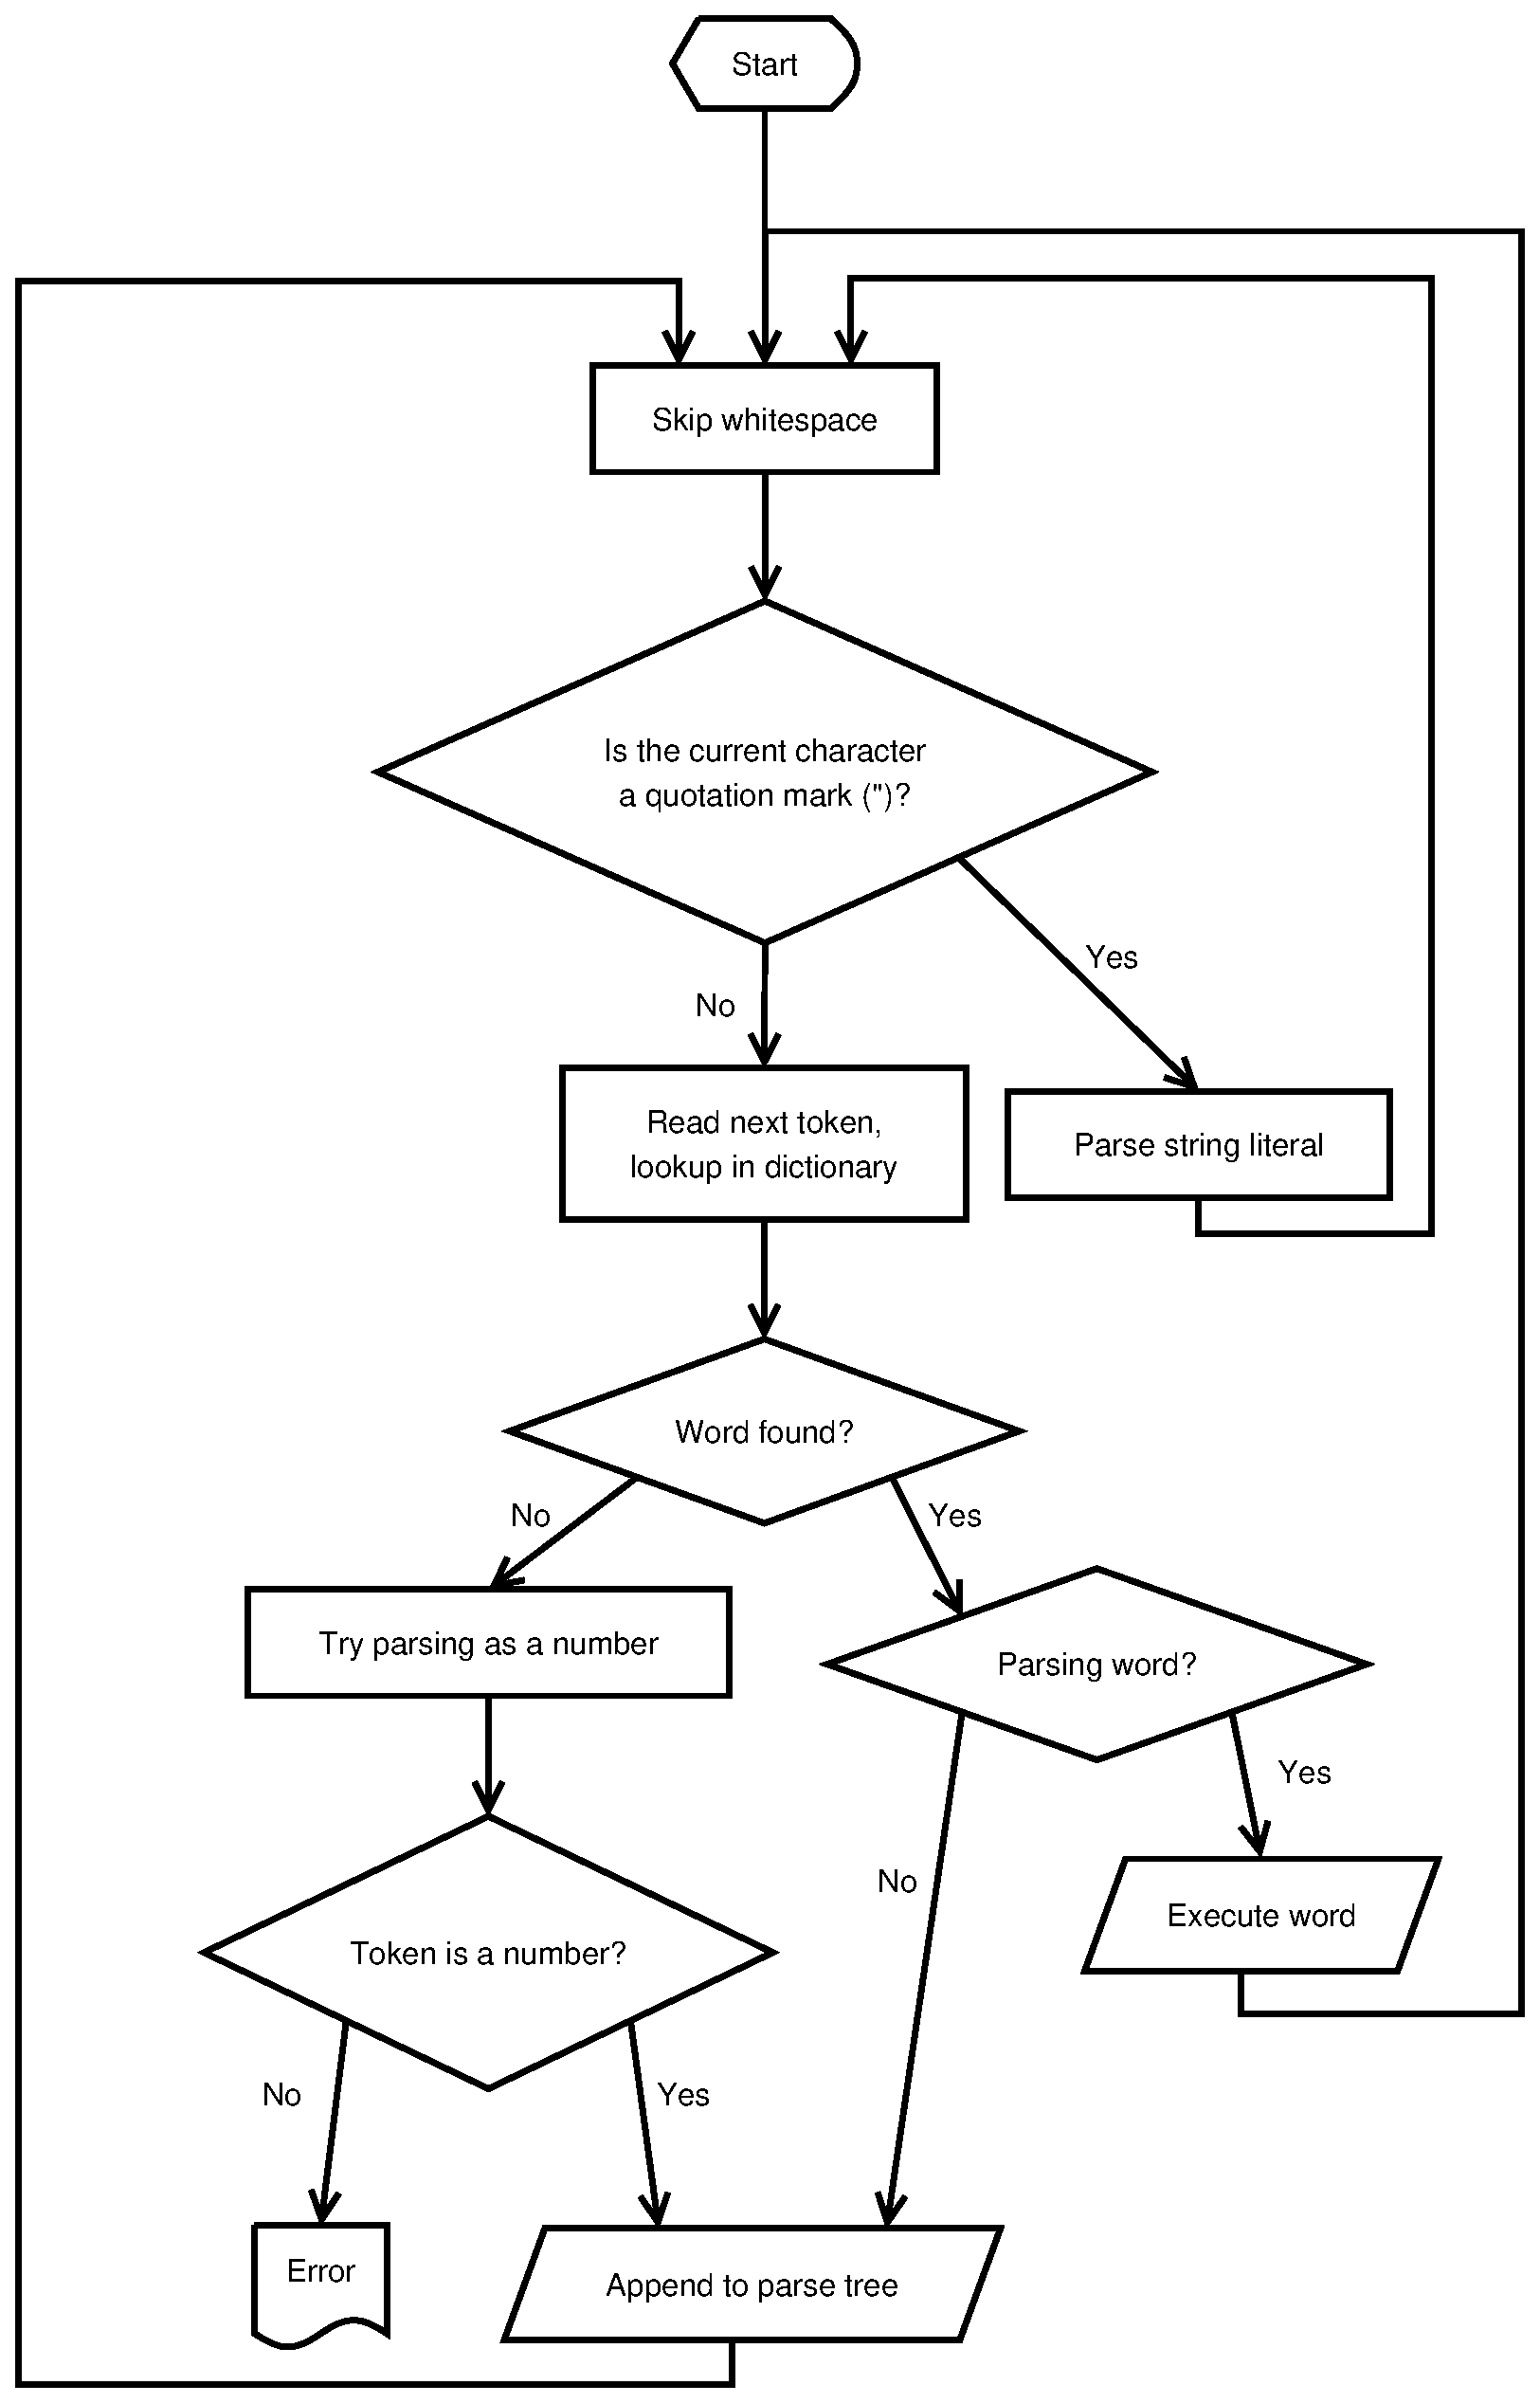
\epsfig{file=parser.eps}}
\end{center}
\end{figure}

At the most abstract level,
Factor syntax consists of whitespace-separated tokens. The parser tokenizes the input on whitespace boundaries, where whitespace is defined as a sequence or one or more space, tab, newline or carriage-return characters.  The parser is case-sensitive, so
the following three expressions tokenize differently:
\begin{verbatim}
2X+
2 X +
2 x +
\end{verbatim}
As the parser reads tokens it makes a distinction between numbers, ordinary words, and
parsing words. Tokens are appended to the parse tree, the top level of which is a list
returned by the original parser invocation. Nested levels of the parse tree are created
by parsing words.

Here is the parser algorithm in more detail -- some of the concepts therein will be defined shortly:

\begin{itemize}
\item If the current character is a double-quote (\texttt{"}), the \texttt{"} parsing word is executed, causing a string to be read.
\item Otherwise, the next token is taken from the input. The parser searches for a word named by the token in the currently used set of vocabularies. If the word is found, one of the following two actions is taken:
\begin{itemize}
\item If the word is an ordinary word, it is appended to the parse tree.
\item If the word is a parsing word, it is executed.
\end{itemize}
Otherwise if the token does not represent a known word, the parser attempts to parse it as a number. If the token is a number, the number object is added to the parse tree. Otherwise, an error is raised and parsing halts.
\end{itemize}

\glossary{name=string mode,
description={a parser mode where token strings are added to the parse tree; the parser will not look up tokens in the dictionary. Activated by switching on the \texttt{string-mode} variable}}

There is one exception to the above process; the parser might be placed in \emph{string mode}, in which case it simply reads tokens and appends them to the parse tree as strings. String mode is activated and deactivated by certain parsing words wishing to read input in an unstructured but tokenized manner -- see \ref{string-mode}.

\glossary{name=parsing word,
description={a word that is run at parse time. Parsing words can be defined by suffixing the compound definition with \texttt{parsing}. Parsing words have the \texttt{\dq{}parsing\dq{}} word property set to true, and respond with true to the \texttt{parsing?}~word}}

Parsing words play a key role in parsing; while ordinary words and numbers are simply
added to the parse tree, parsing words execute in the context of the parser, and can
do their own parsing and create nested data structures in the parse tree. Parsing words
are also able to define new words.

While parsing words supporting arbitrary syntax can be defined, the default set is found
in the \texttt{syntax} vocabulary and provides the basis for all further syntactic
interaction with Factor.

\subsection{\label{vocabsearch}Vocabulary search}

\newcommand{\wordglos}{\glossary{
name=word,
description={an object holding a code definition and set of properties. Words are organized into vocabularies, and are uniquely identified by name within a vocabulary.}}}
\wordglos
\newcommand{\vocabglos}{\glossary{
name=vocabulary,
description={a collection of words, uniquely identified by name. The hashtable of vocabularies is stored in the \texttt{vocabularies} global variable, and the \texttt{USE:}~and \texttt{USING:}~parsing words add vocabularies to the parser's search path}}}
\vocabglos

A \emph{word} associates a code definition with its name. Words are organized into \emph{vocabularies}. Vocabularies are organized into vocabularies. Words are discussed in depth in \ref{words}.

When the parser reads a token, it attempts to look up a word named by that token. The
lookup is performed in the parser's current vocabulary set. By default, this set includes
two vocabularies:
\begin{verbatim}
syntax
scratchpad
\end{verbatim}
The \texttt{syntax} vocabulary consists of a set of parsing words for reading Factor data
and defining new words. The \texttt{scratchpad} vocabulary is the default vocabulary for new
word definitions.
\wordtable{
\parsingword{USE:}{USE: \emph{vocabulary}}{syntax}
}
\newcommand{\useglos}{\glossary{
name=search path,
description={the list of vocabularies that the parser looks up tokens in. You can add to this list with the \texttt{USE:} and \texttt{USING:} parsing words}}}
\useglos

The \texttt{USE:} parsing word adds a new vocabulary at the front of the search path. Subsequent word lookups by the parser will search this vocabulary first.
\begin{alltt}
USE: lists
\end{alltt}
\wordtable{
\parsingword{USING:}{USING: \emph{vocabularies} ;}{syntax}
}
Consecutive \texttt{USE:} declarations can be merged into a single \texttt{USING:} declaration.
\begin{alltt}
USING: lists strings vectors ;
\end{alltt}

Due to the way the parser works, words cannot be referenced before they are defined; that is, source files must order definitions in a strictly bottom-up fashion. For a way around this, see \ref{deferred}.

\subsection{Numbers}

\newcommand{\numberglos}{\glossary{
name=number,
description={an instance of the \texttt{number} class}}}
\numberglos

If a vocabulary lookup of a token fails, the parser attempts to parse it as a number.

\subsubsection{Integers}

\newcommand{\integerglos}{\glossary{
name=integer,
description={an instance of the \texttt{integer} class, which is a disjoint union of the \texttt{fixnum} and \texttt{bignum} classes}}}
\numberglos

\newcommand{\fixnumglos}{\glossary{
name=fixnum,
description={an instance of the \texttt{fixnum} class, representing a fixed precision integer. On 32-bit systems, an element of the interval $(-2^{-29},2^{29}]$, and on 64-bit systems, the interval $(-2^{-61},2^{61}]$}}}
\fixnumglos

\newcommand{\bignumglos}{\glossary{
name=bignum,
description={an instance of the \texttt{bignum} class, representing an arbitrary-precision integer whose value is bounded by available object memory}}}
\bignumglos

The printed representation of an integer consists of a sequence of digits, optionally prefixed by a sign.
\begin{alltt}
123456
-10
2432902008176640000
\end{alltt}
Integers are entered in base 10 unless prefixed with a base change parsing word.
\wordtable{
\parsingword{BIN:}{BIN: \emph{integer}}{syntax}\\
\parsingword{OCT:}{OCT: \emph{integer}}{syntax}\\
\parsingword{HEX:}{HEX: \emph{integer}}{syntax}
}
\begin{alltt}
\textbf{ok} BIN: 1110 BIN: 1 + .
\textbf{15}
\textbf{ok} HEX: deadbeef 2 * .
\textbf{7471857118}
\end{alltt}

\subsubsection{Ratios}

\newcommand{\ratioglos}{\glossary{
name=ratio,
description={an instance of the \texttt{ratio} class, representing an exact ratio of two integers}}}
\ratioglos

The printed representation of a ratio is a pair of integers separated by a slash (\texttt{/}).
No intermediate whitespace is permitted. Either integer may be signed, however the ratio will be normalized into a form where the denominator is positive and the greatest common divisor
of the two terms is 1.
\begin{alltt}
75/33
1/10
-5/-6
\end{alltt}

\subsubsection{Floats}

\newcommand{\floatglos}{\glossary{
name=float,
description={an instance of the \texttt{float} class, representing an IEEE 754 double-precision floating point number}}}
\floatglos

Floating point numbers contain an optional decimal part, an optional exponent, with
an optional sign prefix on either the significand or exponent.
\begin{alltt}
10.5
-3.1456
7e13
1e-5
\end{alltt}

\subsubsection{Complex numbers}

\newcommand{\complexglos}{\glossary{
name=complex,
description={an instance of the \texttt{complex} class, representing a complex number with real and imaginary components, where both components are real numbers}}}
\complexglos
\wordtable{
\parsingword{hash-curly}{\#\{ \emph{real} \emph{imaginary} \}\#}{syntax}
}
A complex number
is given by two components, a ``real'' part and ''imaginary'' part. The components
must either be integers, ratios or floats.
\begin{verbatim}
#{ 1/2 1/3 }#   ! the complex number 1/2+1/3i
#{ 0 1 }#       ! the imaginary unit
\end{verbatim}

\subsection{Literals}

Many different types of objects can be constructed at parse time via literal syntax. Numbers are a special case since support for reading them is built-in to the parser. All other literals are constructed via parsing words.

If a quotation contains a literal object, the same literal object instance is used each time the quotation executes; that is, literals are ``live''.

\subsubsection{\label{boolean}Booleans}

\newcommand{\boolglos}{
\glossary{
name=boolean,
description={an instance of the \texttt{boolean} class, either \texttt{f} or \texttt{t}. See generalized boolean}}
\glossary{
name=generalized boolean,
description={an object used as a truth value. The \texttt{f} object is false and anything else is true. See boolean}}
\glossary{
name=t,
description={the canonical truth value. The \texttt{t} class, whose sole instance is the \texttt{t} object. Note that the \texttt{t} class is not equal to the \texttt{t} object}}
\glossary{
name=f,
description={the canonical false value; anything else is true. The \texttt{f} class, whose sole instance is the \texttt{f} object. Note that the \texttt{f} class is not equal to the \texttt{f} object}}
}
\boolglos
Any Factor object may be used as a truth value in a conditional expression. The \texttt{f} object is false and anything else is true. The \texttt{f} object is also used to represent the empty list, as well as the concept of a missing value. The canonical truth value is the \texttt{t} object.
\wordtable{
\parsingword{f}{f}{syntax}\\
\parsingword{t}{t}{syntax}
}
Adds the \texttt{f} and \texttt{t} objects to the parse tree.

Note that the \texttt{f} parsing word and class is not the same as the \texttt{f} object. The former can be obtained by writing \texttt{\bs~f} inside a quotation, or \texttt{POSTPONE: f} inside a list that will not be evaluated.
\begin{alltt}
\textbf{ok} f \bs f = .
\textbf{f}
\end{alltt}
An analogous distinction holds for the \texttt{t} class and object.

\subsubsection{\label{syntax:char}Characters}

\newcommand{\charglos}{\glossary{
name=character,
description={an integer whose value denotes a Unicode code point. Character values are limited to the range from $0$ to $2^16-1$ inclusive, however in a later release this can be upgraded to the full 21-bit Unicode space without requiring any changes to user code}}}
\charglos
Factor has no distinct character type, however Unicode character value integers can be
read by specifying a literal character, or an escaped representation thereof.
\wordtable{
\parsingword{CHAR:}{CHAR: \emph{token}}{syntax}
}
Adds the Unicode code point of the character represented by \emph{token} to the parse tree.

\newcommand{\escapeglos}{\glossary{
name=escape,
description={a sequence allowing a non-literal character to be inserted in a string. For a list of escapes, see \ref{escape}}}}
\escapeglos
If the token is a single-character string other than whitespace or backslash, the character is taken to be this token. If the token begins with a backslash, it denotes one of the following escape codes.
\begin{table}[Special character escape codes]
\label{escape}
\begin{tabular}{l|l}
Escape code&Character\\
\hline
\texttt{\bs{}\bs}&Backslash (\texttt{\bs})\\
\texttt{\bs{}s}&Space\\
\texttt{\bs{}t}&Tab\\
\texttt{\bs{}n}&Newline\\
\texttt{\bs{}t}&Carriage return\\
\texttt{\bs{}0}&Null byte (ASCII 0)\\
\texttt{\bs{}e}&Escape (ASCII 27)\\
\texttt{\bs{}"}&Double quote (\texttt{"})\\
\end{tabular}
\end{table}
Examples:
\begin{alltt}
\textbf{ok} CHAR: a .
\textbf{97}
\textbf{ok} CHAR: \bs{}0 .
\textbf{0}
\textbf{ok} CHAR: \bs{}n .
\textbf{10}
\end{alltt}
A Unicode character can be specified by its code number by writing \texttt{\bs{}u} followed by a four-digit hexadecimal. That is, the following two expressions are equivalent:
\begin{alltt}
CHAR: \bs{}u0078
78
\end{alltt}
While not useful for single characters, this syntax is also permitted inside strings.

\subsubsection{\label{string-literals}Strings}

\newcommand{\stringglos}{\glossary{
name=string,
description={an instance of the \texttt{string} class, representing an immutable sequence of characters}}}
\stringglos
\wordtable{
\parsingword{"}{"\emph{string}"}{syntax}
}
Reads from the input string until the next occurrence of
\texttt{"}, and appends the resulting string to the parse tree. String literals cannot span multiple lines.
Strings containing
the \texttt{"} character and various other special characters can be read by
inserting escape sequences as described in \ref{syntax:char}.
\begin{alltt}
\textbf{ok} "Hello world" print
\textbf{Hello world}
\end{alltt}

\subsubsection{\label{listsyntax}Lists}
\newcommand{\listglos}{\glossary{
name=list,
description={an instance of the \texttt{list} class, storing a sequence of elements as a chain of zero or more conses, where the car of each cons is an element, and the cdr is either \texttt{f} or another list}}
\glossary{name=proper list, description=see list}
}
\listglos
\wordtable{
\parsingword{openbracket}{[}{syntax}\\
\parsingword{closebracket}{]}{syntax}
}
Parses a list, whose elements are read between \texttt{[} and \texttt{]} and can include other lists.
\begin{verbatim}
[
    "404" "responder" set
    [ drop no-such-responder ] "get" set
]
\end{verbatim}
\newcommand{\consglos}{\glossary{
name=cons,
description={an instance of the \texttt{cons} class, storing an ordered pair of objects referred to as the car and the cdr}}}
\consglos
\wordtable{
\parsingword{conssyntax}{[[ \emph{car} \emph{cdr} ]]}{syntax}
}
Parses two components making up a cons cell. Note that the lists parsed with \texttt{[} and \texttt{]} are just a special case of \texttt{[[} and \texttt{]]}. The following two lines are equivalent.
\begin{alltt}
[ 1 2 3 ]
[[ 1 [[ 2 [[ 3 f ]] ]] ]]
\end{alltt}
The empty list is denoted by \texttt{f}, along with boolean falsity, and the concept of a missing value. The expression \texttt{[ ]} parses to the same object as \texttt{f}.

\subsubsection{Words}

While words parse as themselves, a word occurring inside a quotation is executed when the quotation is called. Sometimes it is desirable to have a word be pushed on the data stack during the execution of a quotation, usually for reflective access to the word's slots.
\wordtable{
\parsingword{bs}{\bs~\emph{word}}{syntax}
}
Reads the next word from the input string and appends some \emph{code} to the parse tree that pushes the word on the stack when the code is called. The following two lines are equivalent:
\begin{verbatim}
\ length
[ length ] car
\end{verbatim}
\wordtable{
\parsingword{POSTPONE:}{POSTPONE: \emph{word}}{syntax}
}
Reads the next word from the input string and appends the word to the parse tree, even if it is a parsing word. For an word \texttt{foo}, \texttt{POSTPONE: foo} and \texttt{foo} are equivalent; however, if \texttt{foo} is a parsing word, the latter will execute it at parse time, while the former will execute it at runtime. Usually used inside parsing words that wish to delegate some action to a further parsing word.
\begin{alltt}
\textbf{ok} : parsing1
    "Parsing 1" print 2 swons ; parsing
\textbf{ok} : parsing2
    "Parsing 2" print POSTPONE: parsing1 ; parsing
\textbf{ok} [ 1 parsing1 3 ] .
\textbf{Parsing 1}
\textbf{[ 1 2 3 ]}
\textbf{ok} [ 0 parsing2 2 4 ] .
\textbf{Parsing 2}
\textbf{Parsing 1}
\textbf{[ 0 2 4 ]}
\end{alltt}

\subsubsection{Mutable literals}

\newcommand{\mutableglos}{\glossary{name=mutable object,
description=an object whose slot values can be changed}
\glossary{name=immutable object,
description=an object whose slot values cannot be changed}}
\mutableglos

Using mutable object literals in word definitions requires care, since if those objects
are mutated, the actual word definition will be changed, which is in most cases not what you would expect. Strings and lists are immutable; string buffers, vectors, hashtables and tuples are mutable.

\subsubsection{\label{sbuf-literals}String buffers}

\newcommand{\sbufglos}{\glossary{
name=string buffer,
description={an instance of the \texttt{sbuf} class, representing a mutable and growable sequence of characters}}
\glossary{name=sbuf, description=see string buffer}}
\sbufglos
\wordtable{
\parsingword{SBUF}{SBUF" \emph{text}"}{syntax}
}
Reads from the input string until the next occurrence of
\texttt{"}, converts the string to a string buffer, and appends it to the parse tree.
As with strings, the escape codes described in \ref{syntax:char} are permitted.
\begin{alltt}
\textbf{ok} SBUF" Hello world" sbuf>string print
\textbf{Hello world}
\end{alltt}

\subsubsection{\label{vector-literals}Vectors}
\newcommand{\vectorglos}{\glossary{
name=vector,
description={an instance of the \texttt{vector} class, storing a mutable and growable sequence of elements in a contiguous range of memory}}}
\vectorglos
\wordtable{
\parsingword{opencurly}{\{}{syntax}\\
\parsingword{closecurly}{\}}{syntax}
}
Parses a vector, whose elements are read between \texttt{\{} and \texttt{\}}.
\begin{verbatim}
{ 3 "blind" "mice" }
\end{verbatim}

\subsubsection{Hashtables}
\newcommand{\hashglos}{\glossary{
name=hashtable,
description={an instance of the \texttt{hashtable} class, providing a mutable mapping of keys to values}}}
\hashglos
\wordtable{
\parsingword{openccurly}{\{\{}{syntax}\\
\parsingword{closeccurly}{\}\}}{syntax}
}
Parses a hashtable. Elements between \texttt{\{\{} and \texttt{\}\}} must be cons cells, where the car is the key and the cdr is a value.
\begin{verbatim}
{{
    [[ "red" [ 255 0 0 ] ]]
    [[ "green" [ 0 255 0 ] ]]
    [[ "blue" [ 0 0 255 ] ]]
}}
\end{verbatim}

\subsubsection{Tuples}
\newcommand{\tupleglos}{\glossary{
name=tuple,
description={an instance of a user-defined class whose metaclass is the \texttt{tuple} metaclass, storing a fixed set of elements in named slots, with optional delegation method dispatch semantics}}}
\tupleglos
\wordtable{
\parsingword{<<}{<<}{syntax}\\
\parsingword{>>}{>>}{syntax}
}
Parses a tuple. The tuple's class must follow \texttt{<<}. The element after that is always the tuple's delegate. Further elements until \texttt{>>} are specified according to the tuple's slot definition, and an error is raised if an incorrect number of elements is given.
\begin{verbatim}
<< color f 255 0 0 >>
\end{verbatim}

\subsection{\label{comments}Comments}

\wordtable{
\parsingword{!}{!~\emph{remainder of line}}{syntax}
}
The remainder of the input line is ignored if an exclamation mark (\texttt{!}) is read.
\begin{alltt}
! Note that the sequence union does not include lists,
! or user defined tuples that respond to the sequence
! protocol.
\end{alltt}
\wordtable{
\parsingword{hash!}{\#!~\emph{remainder of line}}{syntax}
}
\newcommand{\doccommentglos}{\glossary{
name=documentation comment,
description={a comment describing the usage of a word. Delimited by the \texttt{\#"!} parsing word, they appear at the start of a word definition and are stored in the \texttt{""documentation""} word property}}}
\doccommentglos
Comments that begin with \texttt{\#!} are called \emph{documentation comments}.
A documentation comment has no effect on the generated parse tree, but if it is the first thing inside a word definition, the comment text is appended to the string stored in the word's \texttt{"documentation"} property. Word properties are described in \ref{word-props}.
\wordtable{
\parsingword{(}{( \emph{stack effect} )}{syntax}
}
\glossary{
name=stack effect,
description={A string of the form \texttt{( \emph{inputs} -- \emph{outputs} )}, where the inputs and outputs are a whitespace-separated list of names or types. The top of the stack is the right-most token on both sides.}}
\newcommand{\stackcommentglos}{\glossary{
name=stack effect comment,
description={a comment describing the inputs and outputs of a word. Delimited by \texttt{(} and \texttt{}), they appear at the start of a word definition and are stored in the \texttt{""stack-effect""} word property}}}
\stackcommentglos
Comments delimited by \texttt{(} and \texttt{)} are called \emph{stack effect comments}. By convention they are placed at the beginning of a word definition to document the word's inputs and outputs:
\begin{verbatim}
: push ( element sequence -- )
    #! Push a value on the end of a sequence.
    dup length swap set-nth ;
\end{verbatim}
A stack effect comment has no effect on the generated parse tree, but if it is the first thing inside a word definition, the word's \texttt{"stack-effect"} property is set to the comment text. Word properties are described in \ref{word-props}.

\section{Data and control flow}

\subsection{Shuffle words}

\newcommand{\dsglos}{\glossary{
name=stack,
description=see data stack}
\glossary{
name=data stack,
description={the primary means of passing values between words}}}
\dsglos
Shuffle words are placed between words taking action to rearrange items on the stack
as the next word in the quotation would expect them. Their behavior can be understood entirely in terms of their stack effects.
\wordtable{
\ordinaryword{drop}{drop ( x -- )}{kernel}\\
\ordinaryword{2drop}{drop ( x y -- )}{kernel}\\
\ordinaryword{3drop}{drop ( x y z -- )}{kernel}\\
\ordinaryword{nip}{nip ( x y -- y )}{kernel}\\
\ordinaryword{2nip}{2nip ( x y -- y )}{kernel}\\
\ordinaryword{dup}{dup ( x -- x x )}{kernel}\\
\ordinaryword{2dup}{2dup ( x y -- x y x y )}{kernel}\\
\ordinaryword{3dup}{3dup ( x y z -- x y z x y z )}{kernel}\\
\ordinaryword{dupd}{dupd ( x y -- x x y )}{kernel}\\
\ordinaryword{over}{over ( x y -- x y x )}{kernel}\\
\ordinaryword{pick}{pick ( x y z -- x y z x )}{kernel}\\
\ordinaryword{tuck}{tuck ( x y -- y x y )}{kernel}\\
\ordinaryword{swap}{swap ( x y -- y x )}{kernel}\\
\ordinaryword{2swap}{2swap ( x y z t -- z t x y )}{kernel}\\
\ordinaryword{swapd}{swapd ( x y z -- y x z )}{kernel}\\
\ordinaryword{rot}{rot ( x y z -- y z x )}{kernel}\\
\ordinaryword{-rot}{-rot ( x y z -- z x y )}{kernel}
}
Try to avoid the complex shuffle words such as \texttt{rot} and \texttt{2dup} as much as possible, for they make data flow harder to understand. If you find yourself using too many shuffle words, or you're writing
a stack effect comment in the middle of a compound definition to keep track of stack contents, it is
a good sign that the word should probably be factored into two or
more smaller words.

\subsection{\label{quotations}Quotations}

\newcommand{\csglos}{\glossary{
name=return stack,
description=see call stack}
\glossary{
name=call stack,
description={holds quotations waiting to be called. When a quotation is called with \texttt{call}, or when a compound word is executed, the previous call frame is pushed on the call stack, and the new quotation becomes the current call frame}}}
\csglos
\newcommand{\cfglos}{\glossary{
name=call frame,
description=the currently executing quotation}}
\cfglos
\glossary{
name=interpreter,
description=executes quotations by iterating them and recursing into nested definitions. see compiler}

\begin{figure}
\begin{center}
\caption{Interpreter algorithm}
\scalebox{0.45}{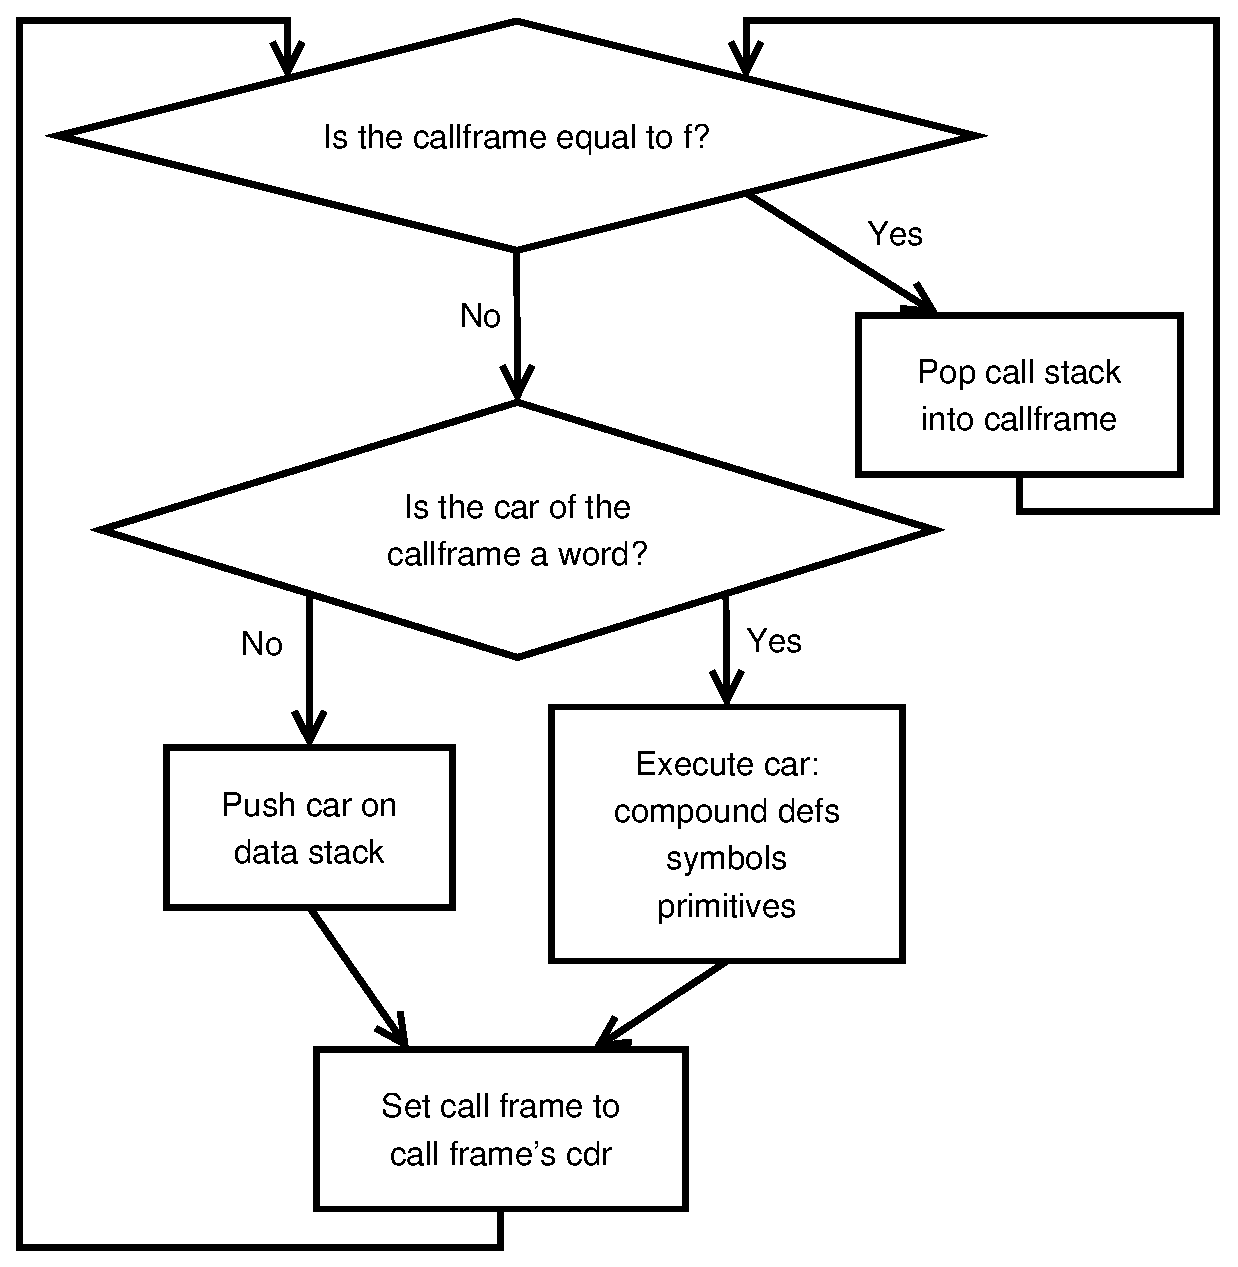
\epsfig{file=interpreter.eps}}
\end{center}
\end{figure}

The Factor interpreter executes quotations. Quotations are lists, and since lists can contain any Factor object, they can contain words. It is words that give quotations their operational behavior, as you can see in the following description of the interpreter algorithm.

\begin{itemize}
\item If the call frame is \texttt{f}, the call stack is popped and becomes the new call frame.
\item If the car of the call frame is a word, the word is executed:
\begin{itemize}
\item If the word is a symbol, it is pushed on the data stack. See \ref{symbols}.
\item If the word is a compound definition, the current call frame is pushed on the call stack, and the new call frame becomes the word definition. See \ref{colondefs}.
\item If the word is compiled or primitive, the interpreter jumps to a machine code definition. See \ref{primitives}.
\item If the word is undefined, an error is raised. See \ref{deferred}.
\end{itemize}
\item Otherwise, the car of the call frame is pushed on the data stack.
\item The call frame is set to the cdr, and the loop continues.
\end{itemize}

The interpreter can be invoked reflectively with the following pair of words.
\wordtable{
\ordinaryword{call}{call ( quot -- )}{kernel}
}
Push the current call frame on the call stack, and set the call stack to the given quotation. Conceptually: calls the quotation, as if its definition was substituted at the location of the \texttt{call}.
\begin{alltt}
\textbf{ok} [ 2 2 + 3 * ] call .
\textbf{12}
\end{alltt}
\wordtable{
\ordinaryword{execute}{execute ( word -- )}{kernel}
}
Execute a word definition, taking action based on the word definition, as above.
\begin{alltt}
\textbf{ok} : hello "Hello world" print ;
\textbf{ok} : twice dup execute execute ;
\textbf{ok} \bs hello twice
\textbf{Hello world}
\textbf{Hello world}
\end{alltt}

\subsubsection{Tail call optimization}

\newcommand{\tailglos}{\glossary{
name=tail call,
description=the last call in a quotation}
\glossary{
name=tail call optimization,
description=the elimination of call stack pushes when making a tail call}}

When a call is made to a quotation from the last word in the call frame, there is no
purpose in pushing the empty call frame on the call stack. Therefore the last call in a quotation does not grow the call stack, and tail recursion executes in bounded space.

\subsubsection{Call stack manipulation}

Because of the way the interpreter is described in \ref{quotations}, the top of the call stack is not accessed during the execution of a quotation; it is only popped when the interpreter reaches the end of the quotation. In effect, the call stack can be used as a temporary storage area, as long as pushes and pops are balanced out within a single quotation.
\wordtable{
\ordinaryword{>r}{>r ( x -- r:x )}{kernel}
}
Moves the top of the data stack to the call stack.
\wordtable{
\ordinaryword{r>}{r> ( x -- r:x )}{kernel}
}
Moves the top of the call stack to the data stack.

The top of the data stack is ``hidden'' between \texttt{>r} and \texttt{r>}.
\begin{alltt}
\textbf{ok} 1 2 3 >r .s r>
\textbf{2
1}
\end{alltt}
It is very important to balance usages of \texttt{>r} and \texttt{r>} within a single quotation or word definition.
\begin{verbatim}
: the-good >r 2 + r> * ; ! Okay
: the-bad  >r 2 + ;      ! Runtime error
: the-ugly r> ;          ! Runtime error
\end{verbatim}
Basically, the rule is you must leave the call stack in the same state as you found it, so that when the current quotation finishes executing, the interpreter can return to the caller.

One exception is that when \texttt{ifte} occurs as the last word in a definition, values may be pushed on the call stack before the condition value is computed, as long as both branches of the \texttt{ifte} pop the values off the call stack before returning.
\begin{verbatim}
: foo ( m ? n -- m+n/n )
    >r [ r> + ] [ drop r> ] ifte ; ! Okay
\end{verbatim}

\subsubsection{Quotation variants}

There are three words that combine shuffle words with \texttt{call}. They are useful in the implementation of higher-order words taking quotations as inputs.
\wordtable{
\ordinaryword{slip}{slip ( quot x -- x | quot: -- )}{kernel}
}
Call a quotation, while hiding the top of the stack. The implementation is as you would expect.
\begin{verbatim}
: slip ( quot x -- x | quot: -- )
    >r call r> ; inline
\end{verbatim}
\wordtable{
\ordinaryword{keep}{keep ( x quot -- x | quot:~x -- )}{kernel}
}
Call a quotation with a value on the stack, restoring the value when the quotation returns.
\begin{verbatim}
: keep ( x quot -- x | quot: x -- )
    over >r call r> ; inline
\end{verbatim}
\wordtable{
\ordinaryword{2keep}{2keep ( x y q -- x y | q:~x y -- )}{kernel}
}
Call a quotation with a pair of values on the stack, restoring the values when the quotation returns.
\begin{verbatim}
: 2keep ( x y quot -- x y | quot: x y -- )
    over >r pick >r call r> r> ; inline
\end{verbatim}

\subsection{Conditionals}

The simplest style of a conditional form is the \texttt{ifte} word.
\wordtable{
\ordinaryword{ifte}{ifte ( cond true false -- )}{kernel}
}
The \texttt{cond} is a generalized boolean. If it is \texttt{f}, the \texttt{false} quotation is called, and if \texttt{cond} is any other value, the \texttt{true} quotation is called. The condition flag is removed from the stack before either quotation executes.

Note that in general, both branches should have the same stack effect. Not only is this good style that makes the word easier to understand, but also unbalanced conditionals cannot be compiled.
\wordtable{
\ordinaryword{when}{when ( cond true -- | true:~-- )}{kernel}\\
\ordinaryword{unless}{unless ( cond false -- | false:~-- )}{kernel}
}
This pair are minor variations on \texttt{ifte} where only one branch is specified. The other is implicitly \texttt{[ ]}. They are implemented in the trivial way:
\begin{verbatim}
: when [ ] ifte ; inline
: unless [ ] swap ifte ; inline
\end{verbatim}
The \texttt{ifte} word removes the condition flag from the stack before calling either quotation. Sometimes this is not desirable, if the condition flag is serving a dual purpose as a value to be consumed by the \texttt{true} quotation. The \texttt{ifte*} word exists for this purpose.
\wordtable{
\ordinaryword{ifte*}{ifte*~( cond true false -- )}{kernel}\\
\texttt{true:~cond --}\\
\texttt{false:~--}
}
If the condition is true, it is retained on the stack before the \texttt{true} quotation is called. Otherwise, the condition is removed from the stack and the \texttt{false} quotation is called. The following two lines are equivalent:
\begin{verbatim}
X [ Y ] [ Z ] ifte*
X dup [ Y ] [ drop Z ] ifte
\end{verbatim}
\wordtable{
\ordinaryword{when*}{when*~( cond true -- | true:~cond -- )}{kernel}\\
\ordinaryword{unless*}{unless*~( cond false -- | false:~-- )}{kernel}
}
These are variations of \texttt{ifte*} where one of the quotations is \texttt{[ ]}.

There is one final conditional form that is used to implement the ``default value'' idiom.
\wordtable{
\ordinaryword{?ifte}{?ifte ( default cond true false -- )}{kernel}\\
\texttt{true:~cond --}\\
\texttt{false:~default --}
}
If the condition is \texttt{f}, the \texttt{false} quotation is called with the \texttt{default} value on the stack. Otherwise, the \texttt{true} quotation is called with the condition on the stack. The following two lines are equivalent:
\begin{verbatim}
X [ Y ] [ Z ] ?ifte
X dup [ nip Y ] [ drop Z ] ifte
\end{verbatim}

\subsubsection{Boolean logic}

The \texttt{?}~word chooses between two values, rather than two quotations.
\wordtable{
\ordinaryword{?}{?~( cond true false -- true/false )}{kernel}
}
It is implemented in the obvious way.
\begin{verbatim}
: ? ( cond t f -- t/f )
    rot [ drop ] [ nip ] ifte ; inline
\end{verbatim}
Several words use \texttt{?}~to implement typical boolean algebraic operations.
\wordtable{
\ordinaryword{>boolean}{>boolean ( obj -- t/f )}{kernel}
}
Convert a generalized boolean into a boolean. That is, \texttt{f} retains its value, whereas anything else becomes \texttt{t}.
\wordtable{
\ordinaryword{not}{not ( ?~-- ?~)}{kernel}
}
Given \texttt{f}, outputs \texttt{t}, and on any other input, outputs \texttt{f}.
\wordtable{
\ordinaryword{and}{and ( ?~?~-- ?~)}{kernel}
}
Outputs \texttt{t} if both of the inputs are true.
\wordtable{
\ordinaryword{or}{or ( ?~?~-- ?~)}{kernel}
}
Outputs \texttt{t} if at least one of the inputs is true.
\wordtable{
\ordinaryword{xor}{xor ( ?~?~-- ?~)}{kernel}
}
Outputs \texttt{t} if exactly one of the inputs is true.
\wordtable{
\ordinaryword{implies}{implies ( b1~b2~-- ?~)}{kernel}
}
Outputs \texttt{t} if \texttt{b1} is false or both inputs are true.

An alternative set of logical operations operate on individual bits of integers bitwise, rather than generalized boolean truth values. They are documented in \ref{bitwise}.

\subsection{Continuations}

\newcommand{\contglos}{
\glossary{name=continuation,
description=an object representing the future of the computation}}
\contglos
At any point in the execution of a Factor program, the \emph{current continuation} represents the future of the computation. This object can be captured with the \texttt{callcc0} and \texttt{callcc1} words.
\wordtable{
\ordinaryword{callcc0}{callcc0 ( quot -- )}{kernel}\\
\texttt{quot:~cont --}\\
\texttt{cont:~--}\\
\ordinaryword{callcc1}{callcc1 ( quot -- )}{kernel}\\
\texttt{quot:~cont --}\\
\texttt{cont:~obj --}
}
Calling one of these words calls the given quotation with the continuation on the stack. The continuation is itself a quotation, and calling it \emph{continues execution} at the point after the call to \texttt{callcc0} and \texttt{callcc1}. Essentially, a continuation is a snapshot of the four stacks that can be restored at a later time.

The difference between \texttt{callcc0} and \texttt{callcc1} lies in the continuation object. When \texttt{callcc1} is used, calling the continuation takes one value from the top of the data stack, and places it back on the \emph{restored} data stack. This allows idioms such as exception handling, co-routines and generators to be implemented via continuations.

\subsubsection{\label{exceptions}Handling exceptional situations}
\glossary{name=exception,
description=an object representing an exceptional situation that has been detected}

Support for handling exceptional situations such as bad user input, implementation bugs, and input/output errors is provided by a pair of words, \texttt{throw} and \texttt{catch}.
\wordtable{
\ordinaryword{throw}{throw ( exception -- )}{errors}
}
Raises an exception. Execution does not continue at the point after the \texttt{throw} call. Rather, the innermost catch block is invoked, and execution continues at that point. Passing \texttt{f} as an exception will cause \texttt{throw} to do nothing.
\wordtable{
\ordinaryword{catch}{catch ( try handler -- )}{errors}\\
\texttt{handler:~exception/f -- }
}
An exception handler is established, and the \texttt{try} quotation is called.

If the \texttt{try} quotation throws an error and no nested \texttt{catch} is established, the following sequence of events takes place:
\begin{itemize}
\item the stacks are restored to their state prior to the \texttt{catch} call,
\item the exception is pushed on the data stack,
\item the \texttt{handler} quotation is called.
\end{itemize}
If the \texttt{try} quotation completes successfully, the stacks are \emph{not} restored. The \texttt{f} object is pushed, and the \texttt{handler} quotation is called.

A common idiom is that the \texttt{catch} block cleans up from the error in some fashion, then passes it on to the next-innermost catch block. The following word is used for this purpose.
\wordtable{
\ordinaryword{rethrow}{throw ( exception -- )}{errors}
}
Raises an exception, without saving the current stacks for post-mortem inspection. This is done so that inspecting the error stacks sheds light on the original cause of the exception, rather than the point where it was rethrown.

Here is a simple example of a word definition that attempts to convert a string representing a hexadecimal number into an integer, and instead of halting execution when the string is not valid, it simply outputs \texttt{f}.
\begin{verbatim}
: catch-hex> ( str -- n/f )
    [ hex> ] [ [ drop f ] when ] catch ;
\end{verbatim}
Exception handling is implemented using a \emph{catch stack}. The \texttt{catch} word pushes the current continuation on the catch stack, and \texttt{throw} calls the continuation at the top of the catch stack with the raised exception.
\glossary{name=catch stack,
description={a stack of exception handler continuations, pushed and popped by \texttt{catch}}}

\subsubsection{Multitasking}

Factor implements co-operative multitasking, where the thread of control switches between tasks at explicit calls to \texttt{yield}, as well as when blocking I/O is performed. Multitasking is implemented via continuations.
\wordtable{
\ordinaryword{in-thread}{in-thread ( quot -- )}{threads}
}
Calls \texttt{quot} in a co-operative thread. The new thread begins executing immediately, and the current thread resumes when the quotation yields, either from blocking
I/O or an explicit call to \texttt{yield}. This is implemented by adding the current continuation to the run queue, then calling \texttt{quot}, and finally executing \texttt{stop} after \texttt{quot} returns.
\wordtable{
\ordinaryword{yield}{yield ( -- )}{threads}
}
Add the current continuation to the end of the run queue, and call the continuation at the front of the run queue.
\wordtable{
\ordinaryword{stop}{stop ( -- )}{threads}
}
Call the continuation at the front of run queue, without saving the current continuation. In effect, this stops the current thread.

\subsubsection{Interpreter state}

The current state of the interpreter is determined by the contents of the four stacks. A set of words for getting and setting stack contents are the primitive building blocks for continuations, and in turn abstractions such as exception handling and multitasking.
\wordtable{
\ordinaryword{datastack}{datastack ( -- vector )}{kernel}\\
\ordinaryword{set-datastack}{set-datastack ( vector -- )}{kernel}
}
Save and restore the data stack contents. As an example, here is a word that executes a quotation and restores the data stack to its previous state;
\begin{verbatim}
: keep-datastack
    ( quot -- ) datastack slip set-datastack drop ;
\end{verbatim}
Note that the \texttt{drop} call is made to remove the original quotation from the stack.
\wordtable{
\ordinaryword{callstack}{callstack ( -- vector )}{kernel}\\
\ordinaryword{set-callstack}{set-callstack ( vector -- )}{kernel}
}
Save and restore the call stack contents. The call stack does not include the currently executing quotation that made the call to \texttt{callstack}, since the current quotation is held in the call frame -- \ref{quotations} has details. Similarly, calling \texttt{set-callstack} will continue executing the current quotation until it returns, at which point control transfers to the quotation at the top of the new call stack.
\wordtable{
\ordinaryword{namestack}{namestack ( -- list )}{namespaces}\\
\ordinaryword{set-namestack}{set-namestack ( list -- )}{namespaces}
}
Save and restore the name stack, used for dynamic variable bindings. See \ref{namespaces}.
\wordtable{
\ordinaryword{catchstack}{catchstack ( -- list )}{errors}\\
\ordinaryword{set-catchstack}{set-catchstack ( list -- )}{errors}
}
Save and restore the catch stack, used for exception handling. See \ref{exceptions}.

\section{\label{words}Words}

\wordglos
\vocabglos
\glossary{name=defining word,
description=a word that adds definitions to the dictionary}
\glossary{name=dictionary,
description=the collection of vocabularies making up the code in the Factor image}
Words are the fundamental unit of code in Factor, analogous to functions or procedures in other languages. Words are also objects, and this concept forms the basis for Factor's meta-programming facilities. Words hold two distinct pieces of information:
\begin{itemize}
\item A definition, specifying the behavior of the word when executed,
\item A set of word properties, including the name of the word, its vocabulary, any documentation strings, and other meta-data.
\end{itemize}
\wordtable{
\ordinaryword{word?}{word?~( object -- ?~)}{words}
}
Tests if the \texttt{object} is a word.
\wordtable{
\classword{word}{words}
}
The class of words.

\subsection{Vocabularies}
\wordtable{
\symbolword{vocabularies}{words}
}
Words are organized into named vocabularies, stored in the global \texttt{vocabularies} variable.
\wordtable{
\parsingword{IN:}{IN:~\emph{vocabulary}}{syntax}
}
Sets the current vocabulary for new word definitions, and adds the vocabulary to the search path (\ref{vocabsearch}).

Parsing words add definitions to the current vocabulary. When a source file is being parsed, the current vocabulary is initially set to \texttt{scratchpad}.

\subsubsection{Searching for words}

Words whose names are known at parse time -- that is, most words making up your program -- can be referenced by stating their name. However, the parser itself, and sometimes code you write, will need to look up words dynamically.
\wordtable{
\ordinaryword{search}{search ( name vocabs -- word )}{words}
}
The \texttt{vocabs} parameter is a list of vocabulary names. If a word with the given name is found, it is pushed on the stack, otherwise, \texttt{f} is pushed.

\subsubsection{Creating words}

\wordtable{
\ordinaryword{create}{create ( name vocabulary -- word )}{words}
}
Creates a new word \texttt{name} in \texttt{vocabulary}. If the vocabulary already contains a word with this name, the existing word is returned.
\wordtable{
\ordinaryword{create-in}{create-in ( name -- word )}{words}
}
Creates a new word \texttt{name} in the current vocabulary. Should only be called from parsing words (\ref{parsing-words}), and in fact is defined as:
\begin{verbatim}
: create-in ( name -- word ) "in" get create ;
\end{verbatim}

\subsection{Word definition}

There are two ways to create a word definition:
\begin{itemize}
\item Using parsing words at parse time,
\item Using defining words at run-time. This is a more dynamic feature that can be used to implement code generation and such, and in fact parse-time defining words are implemented in terms of run-time defining words.
\end{itemize}

\subsubsection{\label{colondefs}Compound definitions}

\newcommand{\colonglos}{\glossary{
name=compound definition,
description=a word defined to execute a quotation consisting of existing words}
\glossary{
name=colon definition,
description=see compound definition}}
\colonglos
A compound definition associates a word name with a quotation that is called when the word is executed.
\wordtable{
\parsingword{:}{:~\emph{name} \emph{definition} ;}{syntax}
}
A word \texttt{name} is created in the current vocabulary, and is associated with \texttt{definition}.
\begin{verbatim}
: ask-name ( -- name )
    "What is your name? " write read-line ;
: greet ( name -- )
    "Greetings, " write print ;
: friend ( -- )
    ask-name greet ;
\end{verbatim}
By convention, the word name should be followed by a stack effect comment, and for more complex definitions, a documentation comment; see \ref{comments}.
\wordtable{
\ordinaryword{define-compound}{define-compound ( word quotation -- )}{words}
}
Defines \texttt{word} to call the \texttt{quotation} when executed.
\wordtable{
\ordinaryword{compound?}{compound?~( object -- ?~)}{words}
}
Tests if the \texttt{object} is a compound word definition.
\wordtable{
\classword{compound}{words}
}
The class that all compound words are an instance of.

\subsubsection{\label{symbols}Symbols}

\newcommand{\symbolglos}{\glossary{
name=symbol,
description={a word defined to push itself on the stack when executed, created by the \texttt{SYMBOL:}~parsing word}}}
\symbolglos
\wordtable{
\parsingword{SYMBOL:}{SYMBOL:~\emph{name}}{syntax}
}
A word \texttt{name} is created in the current vocabulary that pushes itself on the stack when executed. Symbols are used to identify variables (\ref{namespaces}) as well as for storing crufties in their properties (\ref{word-props}).
\wordtable{
\ordinaryword{define-symbol}{define-symbol ( word -- )}{words}
}
Defines \texttt{word} to push itself on the data stack when executed.
\wordtable{
\ordinaryword{symbol?}{symbol?~( object -- ?~)}{words}
}
Tests if the \texttt{object} is a symbol.
\wordtable{
\classword{symbol}{words}
}
The class that all symbols are an instance of.

\subsubsection{\label{primitives}Primitives}
\newcommand{\primglos}{\glossary{
name=primitive,
description=a word implemented as native code in the Factor runtime}}
\symbolglos

Executing a primitive invokes native code in the Factor runtime. Primitives cannot be defined through Factor code. Compiled definitions behave similarly to primitives in that the interpreter jumps to native code upon encountering them.
\wordtable{
\ordinaryword{primitive?}{primitive?~( object -- ?~)}{words}
}
Tests if the \texttt{object} is a primitive.
\wordtable{
\classword{primitive}{words}
}
The class that all primitives are an instance of.

\subsubsection{\label{deferred}Deferred words and mutual recursion}

\glossary{
name=deferred word,
description={a word without a definition, created by the \texttt{DEFER:}~parsing word}}
Due to the way the parser works, words cannot be referenced before they are defined; that is, source files must order definitions in a strictly bottom-up fashion. Mutually-recursive pairs of words can be implemented by \emph{deferring} one of the words in the pair so that the second word in the pair can parse, then by replacing the deferred definition with a real one.
A demonstration of the idiom:
\begin{verbatim}
DEFER: foe
: fie ... foe ... ;
: foe ... fie ... ;
\end{verbatim}
\wordtable{
\parsingword{DEFER:}{DEFER:~\emph{name}}{syntax}
}
Create a word \texttt{name} in the current vocabulary that simply raises an error when executed. Usually, the word will be replaced with a real definition later.
\wordtable{
\ordinaryword{undefined?}{undefined?~( object -- ?~)}{words}
}
Tests if the \texttt{object} is an undefined (deferred) word.
\wordtable{
\classword{undefined}{words}
}
The class that all undefined words are an instance of.

\subsubsection{Undefining words}

\wordtable{
\parsingword{FORGET:}{FORGET:~\emph{name}}{syntax}
}
Removes the word \texttt{name} from its vocabulary. Existing definitions that reference the word will continue to work, but newly-parsed occurrences of the word will not locate the forgotten definition. No exception is thrown if no such word exists.
\wordtable{
\ordinaryword{forget}{forget ( word -- )}{words}
}
Removes the word from its vocabulary. The parsing word \texttt{FORGET:} is implemented using this word.

\subsection{\label{word-props}Word properties}

\glossary{name=word property,
description={a name/value pair stored in a word's properties}}
\glossary{name=word properties,
description={a hashtable associated with each word storing various sundry properties}}

Each word has an associated hashtable of properties. Conventionally, the property names are strings, but nothing requires that this be so.

A common idiom in the Factor library is to use symbols for their properties. 

\wordtable{
\ordinaryword{word-prop}{word-prop ( word name -- value )}{words}\\
\ordinaryword{set-word-prop}{set-word-prop ( value word name -- )}{words}
}
Retrieve and store word properties. Note that the stack effect is designed so that it is most convenient when \texttt{name} is a literal that is pushed on the stack right before executing these words. This is usually the case.

\wordtable{
\ordinaryword{word-name}{word-prop ( word -- name )}{words}\\
\ordinaryword{word-vocabulary}{word-vocabulary ( word -- vocabulary )}{words}
}
Retreive the name of a word, and the name of the vocabulary it is stored in. The definitions are trivial:
\begin{verbatim}
: word-name "name" word-prop ;
: word-vocabulary "vocabulary" word-prop ;
\end{verbatim}

\wordtable{
\ordinaryword{word-sort}{word-sort ( list -- list )}{words}
}
Sort a list of words by name.

\wordtable{
\ordinaryword{word-props}{word-props ( word -- hashtable )}{words}\\
\ordinaryword{set-word-props}{set-word-props ( hashtable word -- )}{words}
}
Retreive and store the entire set of word properties.

\subsection{Low-level details}

The actual behavior of a word when executed is determined by the values of two slots:
\begin{itemize}
\item The primitive number
\item The primitive parameter
\end{itemize}
The primitive number is an index into an array of native functions in the Factor runtime.
Some frequently-occurring primitive numbers:
\begin{description}
\item[0] deferred word,
\item[1] compound definition -- executes the quotation stored in the parameter slot,
\item[2] symbol -- pushes the value of the parameter slot,
\item[3 onwards] the actual set of primitives, of which there are around 170.
\end{description}
The words outlined in this section should not be used in ordinary code.
\wordtable{
\ordinaryword{word-primitive}{word-primitive ( word -- n )}{words}\\
\ordinaryword{set-word-primitive}{set-word-primitive ( word -- n )}{words}
}
Retrieves and stores a word's primitive number.

\wordtable{
\ordinaryword{word-def}{word-def ( word -- object )}{words}\\
\ordinaryword{set-word-def}{set-word-def ( object word -- )}{words}
}
Retrieves and stores a word's primitive parameter. This parameter is only used if the primitive number is 1 (compound definitions) or 2 (symbols). Note that to define a compound definition or symbol, you must use \texttt{define-compound} or \texttt{define-symbol}, as these words do not update the cross-referencing of word dependencies.

\wordtable{
\ordinaryword{word-xt}{word-xt ( word -- n )}{words}\\
\ordinaryword{set-word-xt}{set-word-xt ( n word -- )}{words}
}
Retrieves and stores a word's \emph{execution token}.

This is an even lower-level facility for working with the address containing native code to be invoked when the word is executed. The compiler sets the execution token to a location in memory containing generated code.

\wordtable{
\ordinaryword{update-xt}{update-xt ( word -- )}{words}
}
Updates a word's execution token according to its primitive number. When called with a compiled word, has the effect of decompiling the word. The execution token is automatically updated after a call to \texttt{set-word-primitive}.

\wordtable{
\ordinaryword{recrossref}{recrossref ( word -- )}{words}
}
Updates the cross-referencing database, which you will probably need to do if you mess around with any of the words in this section -- assuming Factor does not crash first, that is.

\chapter{The library}

\section{Objects}

\glossary{name=object,
description=a datum that can be identified}
\mutableglos

Everything in Factor is an object, where an object is a collection of slots. Each object has a unique identity, and references to objects are passed by value on the stack. It is possible to have two references to the same object, and if the object is mutated through one reference, the changes will be visible through the other reference. Not all objects are mutable; the documentation for each class details if its instances are mutable or not.

\subsection{\label{equality}Identity and equality}

\glossary{name=equal,
description={two objects are equal if they have the same class and if their slots are equal, or alternatively, if both are numbers that denote the same value}}
There are two distinct notions of ``sameness'' when it comes to objects. You can test if two references point to the same object, or you can test if two objects are equal in some sense, usually by having the same type and equal slot values.
\wordtable{
\ordinaryword{eq?}{eq?~( object object -- ?~)}{kernel}
}
Output \texttt{t} if two references point to the same object, and \texttt{f} otherwise.
\wordtable{
\genericword{=}{= ( object object -- ?~)}{kernel}
}
Output \texttt{t} if two objects are equal, and \texttt{f} otherwise. The precise meaning of equality depends on the object's class, however usually two objects are equal if their slot values are equal. If two objects are equal, they have the same printed representation, although the converse is not always true. In particular:
\begin{itemize}
\item If no more specific method is defined, \texttt{=} calls \texttt{eq?}.
\item Two numbers are equal if they have the same numerical value.
\item Two sequences are equal if they are both instances of the same class, and if they have the same length, and elements.
\item Two hashtables are equal if they hold the same set of key/value pairs.
\item Two tuples are equal if they are of the same class and their slots are equal.
\item Two words are equal if they are the same object.
\end{itemize}
\wordtable{
\genericword{clone}{clone ( object -- object )}{kernel}
}
Make a fresh object that is equal to the given object. This is not guaranteed to actually copy the object; it does nothing with immutable objects, and does not copy words either. However, sequences and tuples can be cloned to obtain a new shallow copy of the original.

\subsection{Generic words and methods}

\glossary{name=generic word,
description={a word defined using the \texttt{GENERIC:}~parsing word. The behavior of generic words depends on the class of the object at the top of the stack. A generic word is composed of methods, where each method is specialized on a class}}
\glossary{name=method,
description={gives a generic word behavior when the top of the stack is an instance of a specific class}}
Sometimes  you want a word's behavior to depend on the class of the object at the top of the stack, however implementing the word as a set of nested conditional tests is undesirable since it leads to unnecessary coupling -- adding support for a new class requires modifying the original definition of the word.

A generic word is a word whose behavior depends on the class of the
object at the top of the stack, however this behavior is defined in a
decentralized manner.

\wordtable{
\parsingword{GENERIC:}{GENERIC: \emph{word}}{syntax}
}
Defines a new generic word. Initially, it contains no methods, and thus will raise an error when called.

\wordtable{
\parsingword{M:}{M: \emph{class} \emph{word} \emph{definition} ;}{syntax}
}
Defines a method, that is, a behavior for the generic \texttt{word} specialized on instances of \texttt{class}. Each method definition
can potentially occur in a different source file.

\subsubsection{\label{method-order}Method ordering}

If two classes have a non-empty intersection, there is no guarantee that one is a subclass of the other. This means there is no canonical linear ordering of classes. The methods of a generic word are linearly ordered, though, and you can inspect this order using the \texttt{order} word.

Suppose you have the following definitions:
\begin{verbatim}
GENERIC: foo
M: integer foo 1 + ;
M: number foo 1 - ;
M: object foo dup 2list ;
\end{verbatim}
Since the \texttt{integer} class is strictly smaller than the \texttt{number} class, which in turn is strictly smaller than the \texttt{object} class, the ordering of methods is not surprising in this case:
\begin{alltt}
\textbf{ok} \bs foo order .
\textbf{[ object number integer ]}
\end{alltt}
However, suppose we had the following set of definitions:
\begin{verbatim}
GENERIC: describe
M: general-t describe drop "a true value" print ;
M: general-list describe drop "a list" print ;
M: object describe drop "an object" print ;
\end{verbatim}
Neither \texttt{general-t} nor \texttt{general-list} contains the other, and their intersection is the non-empty \texttt{cons} class. So the generic word system will place \texttt{object} first in the method order, however either \texttt{general-t} or \texttt{general-list} may come next, and it is pretty much a random choice that depends on hashing:
\begin{alltt}
\textbf{ok} \bs bar order .
\textbf{[ object general-list general-t ]}
\end{alltt}

Therefore, the outcome of calling \texttt{bar} with a cons cell is undefined.

\subsection{Classes}
\glossary{name=class,
description=a set of objects defined in a formal manner. Methods specialize generic words on classes}
\glossary{name=metaclass,
description={a set of classes sharing common traits. Examples include \texttt{builtin}, \texttt{union}, and \texttt{tuple}}}

\wordtable{
\classword{object}{generic}
}
Every object is a member of the \texttt{object} class. If you provide a method specializing
on the \texttt{object} class for some generic word, the method will be
invoked when no more specific method exists. For example:
\begin{verbatim}
GENERIC: describe
M: number describe
    "The number " write . ;
M: object describe
    "I don't know anything about " write . ;
\end{verbatim}
Each class has a membership predicate named
after the class with a \texttt{?}~suffix, with the following exceptions:
\begin{description}
\item[object] there is no need for a predicate word, since
every object is an instance of this class.
\item[f] the only instance of this class is the singleton
\texttt{f} signifying falsity, missing value, and empty list, and the predicate testing for this is the built-in library word \texttt{not}.
\item[t] the only instance of this class is the canonical truth value
\texttt{t}. You can write \texttt{t =} to test for this object, however usually
any object distinct from \texttt{f} is taken as a truth value, and \texttt{t} is not tested for directly.
\end{description}

\subsubsection{Built-in classes}
\glossary{name=type,
description={an object invariant that describes its shape. An object's type is constant for the lifetime of the object, and there is only a fixed number of types built-in to the run-time. See class}}
\glossary{name=built-in class,
description=see type}
Every object is an instance of to exactly one type, and the type is constant for the lifetime of the object. There is only a fixed number of types built-in to the run-time, and corresponding to each type is a \emph{built-in class}:
\begin{verbatim}
alien
array
bignum
byte-array
complex
cons
dll
f
fixnum
float
ratio
sbuf
string
t
tuple
vector
word
\end{verbatim}
\wordtable{
\ordinaryword{type}{type ( object -- n )}{kernel}
}
Outputs the type number of a given object. Most often, the \texttt{class} word is more useful.
\wordtable{
\ordinaryword{class}{class ( object -- class )}{kernel}
}
Outputs the canonical class of a given object. While an object may be an instance of more than one class, the canonical class is either the built-in class, or if the object is a tuple, the tuple class. Examples:
\begin{alltt}
\textbf{ok} 1.0 class .
\textbf{float}
\textbf{ok} TUPLE: point x y z ;
\textbf{ok} << point f 1 2 3 >> class .
\textbf{point}
\end{alltt}

\subsubsection{Unions}
\glossary{name=union,
description={a class whose set of instances is the union of the set of instances of a list of member classes}}
An object is an instance of a union class if it is an instance of one of its members. Union classes are used to associate the same method with several different classes, as well as to conveniently define predicates.
\wordtable{
\parsingword{UNION:}{UNION: \emph{name} \emph{members} ;}{syntax}
}
Defines a union class. For example, the Factor library defines some unions over numeric types:
\begin{verbatim}
UNION: integer fixnum bignum ;
UNION: rational integer ratio ;
UNION: real rational float ;
UNION: number real complex ;
\end{verbatim}
Now, the absolute value function can be defined in an efficient manner
for real numbers, and in a more general fashion for complex numbers:
\begin{verbatim}
GENERIC: abs ( z -- |z| )
M: real abs dup 0 < [ neg ] when ;
M: complex abs >rect mag2 ;
\end{verbatim}

\subsubsection{Complements}
\glossary{name=complement,
description={a class whose set of instances is the set of objects that are not instances of a specific class}}

An object is an instance of a complement if it is not an instance of the complement's parameter.
\wordtable{
\parsingword{COMPLEMENT:}{COMPLEMENT: \emph{name} \emph{parameter}}{syntax}
}
Defines a complement class. For example, the class of all values denoting ``true'' is defined as follows:
\begin{verbatim}
COMPLEMENT: general-t f
\end{verbatim}

\subsubsection{Predicates}
\glossary{name=predicate,
description={a word with stack effect \texttt{( object -- ?~)}, or more alternatively, a class whose instances are the instances of a superclass that satisfy an arbitrary predicate}}
An object is an instance of a predicate classes if it is an instance of the predicate's parent class, and if it satisfies the predicate definition.

Each predicate must be
defined as a subclass of some other class. This ensures that predicates inheriting from disjoint classes do not need to be
exhaustively tested during method dispatch.
\wordtable{
\parsingword{PREDICATE:}{PREDICATE: \emph{parent} \emph{name} \emph{predicate} ;}{syntax}
}
Defines a predicate class deriving from \texttt{parent} whose instances are the instances of \texttt{superclass} that satisfy the \texttt{predicate} quotation. The predicate quotation must have stack effect \texttt{( object -- ?~)}.

For example, the \texttt{strings} vocabulary contains subclasses of \texttt{integer}
classifying various ASCII characters:
\begin{verbatim}
PREDICATE: integer blank     " \t\n\r" str-contains? ;
PREDICATE: integer letter    CHAR: a CHAR: z between? ;
PREDICATE: integer LETTER    CHAR: A CHAR: Z between? ;
PREDICATE: integer digit     CHAR: 0 CHAR: 9 between? ;
PREDICATE: integer printable CHAR: \s CHAR: ~ between? ;
\end{verbatim}

\subsubsection{Operations on classes}
\wordtable{
\ordinaryword{class-and}{class-and ( class class -- class )}{kernel}\\
\ordinaryword{class-or}{class-or ( class class -- class )}{kernel}
}
Intersection and union of classes. Note that the returned class might not be the exact desired class; for example, \texttt{object} is output if no suitable class definition could be found at all.
\wordtable{
\ordinaryword{class<}{class< ( class class -- class )}{kernel}
}
Classes are partially ordered. This ordering determines the method ordering of a generic word (\ref{method-order}).

\subsection{Tuples}
\tupleglos

Tuples are user-defined classes composed of named slots. All tuples have the same type, however distinct classes of tuples are defined.
\wordtable{
\parsingword{TUPLE:}{TUPLE: \emph{name} \emph{slots} ;}{syntax}
}
Defines a new tuple class with membership predicate \texttt{name?}~and constructor \texttt{<name>}.

The constructor takes slots in left-to-right order from the stack. After construction, slots are read and written using various automatically-defined words with names of the
form \texttt{\emph{class}-\emph{slot}} and \texttt{set-\emph{class}-\emph{slot}}.

Here is an example:
\begin{verbatim}
TUPLE: point x y z ;
\end{verbatim}
This defines a new class named \texttt{point}, along with the
following set of words:
\begin{verbatim}
<point> point?
point-x set-point-x
point-y set-point-y
point-z set-point-z
\end{verbatim}
The word \texttt{<point>} takes the slot values from the stack and
produces a new \texttt{point}:
\begin{alltt}
\textbf{ok} 1 2 3 <point> .
\textbf{<< point 1 2 3 >>}
\end{alltt}

\subsubsection{Constructors}

Constructors are named after the tuple class surrounded in angle
brackets (\texttt{<}~and~\texttt{>}). A default constructor is provided
that reads slot values from the stack, however a custom constructor can
be defined using the \texttt{C:} parsing word.
\wordtable{
\parsingword{C:}{C: \emph{class} \emph{definition} ;}{syntax}
}
Define a \texttt{<class>} word that creates a tuple instance of the \texttt{class}, then applies the \texttt{definition} to this new tuple. The \texttt{definition} quotation must have stack effect \texttt{( tuple -- tuple )}.

\subsubsection{Delegation}

\glossary{name=delegate,
description={a fa\,cade object's delegate receives unhandled methods that are called on the fa\,cade}}
\glossary{name={fa\,cade},
description=an object with a delegate}

Each tuple can have an optional delegate tuple. Generic words called on
the tuple that do not have a method for the tuple's class will be passed on
to the delegate. Note that delegation to objects that are not tuples is not fully supported at this stage and might not work as you might expect.
\wordtable{
\ordinaryword{delegate}{delegate ( object -- object )}{syntax}
}
Returns an object's delegate, or \texttt{f} if no delegate is set. Note that in this case,  undefined methods will be passed to \texttt{f}; rather an error is raised immediately.
\wordtable{
\ordinaryword{set-delegate}{set-delegate ( object tuple -- )}{syntax}
}
Sets a tuple's delegate.

Factor uses delegation is used instead of inheritance, but it is not a direct
substitute; in particular, the semantics differ in that a delegated
method call receives the delegate on the stack, not the original object.

\section{Sequences}

\glossary{name=sequence,
description=an object storing a linearly-ordered set of elements}
A sequence is a linearly-ordered collection of objects. A set of built-in sequence types  is provided by the library.

\begin{tabular}[t]{l|c|c|c|c|c|l}
\multicolumn{4}{l|}{}&\multicolumn{2}{c|}{Adding elements}&\multicolumn{1}{l}{}\\
\hline
Class&Mutable&Growable&Lookup&at start&at end&Primary purpose\\
\hline
\texttt{array}&$\surd$&&$O(1)$&&&Low-level and unsafe (\ref{unsafe})\\
\texttt{list}&&&$O(n)$&$O(1)$&$O(n)$&Functional manipulation\\
\texttt{vector}&$\surd$&$\surd$&$O(1)$&$O(n)$&$O(1)$&Imperitive aggregation\\
\texttt{sbuf}&$\surd$&$\surd$&$O(1)$&$O(n)$&$O(1)$&Character accumilation\\
\texttt{string}&&&$O(1)$&&&Immutable text strings
\end{tabular}

Additionally, user-defined classes can implement the sequence protocol and gain the ability to reuse many of the words in this section.

\subsection{Sequence protocol}

The following set of generic words is the core of the sequence protocol. The mutating words are not supported by all sequences; in particular, lists and strings are immutable.

\glossary{name=resizable sequence,
description={a sequence implementing the \texttt{set-length} generic word. For example, vectors and string buffers}}
\glossary{name=mutable sequence,
description={a sequence implementing the \texttt{set-nth} generic word. For example, vectors and string buffers}}
The sequence protocol consists of a set of generic words. Any object that is an instance of a class implementing these generic words can be thought of as a sequence, and given to the words in the following sections.

\wordtable{
\genericword{length}{length ( seq -- n )}{sequences}
}
Outputs the length of the sequence. All sequences support this operation.
\wordtable{
\genericword{set-length}{set-length ( n seq -- )}{sequences}
}
Resizes the sequence. Only vectors and string buffers support this operation.

\wordtable{
\genericword{nth}{nth ( n seq -- elt )}{sequences}
}
Outputs the $n$th element of the sequence. Elements are numbered starting from 0, so the last element has an index one less than the length of the sequence. An exception should be thrown if an out-of-bounds index is accessed. All sequences support this operation, however with lists it has non-constant running time.

\wordtable{
\genericword{set-nth}{set-nth ( elt n seq -- )}{sequences}
}
Sets the $n$th element of the sequence. Storing beyond the end of a resizable sequence such as a vector or string buffer grows the sequence. Storing to a negative index is always an error.

\subsection{Sequence operations}

\subsubsection{Queries}

The following set of operations inspect sequence elements without modifying or creating anything.

\wordtable{
\genericword{empty?}{empty?~( seq -- ?~)}{sequences}
}
Tests if the sequence contains any elements. The default implementation of this word tests if the length is zero; user-defined sequences can provide a custom implementation that is more efficient.
\wordtable{
\ordinaryword{index}{index ( obj seq -- n )}{sequences}
}
Outputs the index of the first element in the sequence equal to \texttt{obj}. If no element is found, outputs $-1$.
\wordtable{
\ordinaryword{index*}{index* ( obj i seq -- n )}{sequences}
}
Outputs the index of the first element in the sequence equal to \texttt{obj}, starting from \texttt{i}. If no element is found, outputs $-1$.
\wordtable{
\ordinaryword{peek}{peek ( sequence -- element )}{sequences}
}
Outputs the last element of the sequence. Throws an exception if the sequence is empty.
\wordtable{
\ordinaryword{sequence=}{sequence= ( s1 s2 -- ?~)}{sequences}
}
Tests if the two sequences have the same length and elements. This is weaker than \texttt{=}, since it does not ensure that the sequences are instances of the same class.

\subsubsection{Functional operations}

The following set of sequence operations do not modify their inputs.

\wordtable{
\ordinaryword{append}{append ( s1 s2 -- seq )}{sequences}
}
Output a new sequence consisting of the elements of \texttt{s1} followed by the elements of \texttt{s2}. The new sequence is of the same class as \texttt{s1}.
\wordtable{
\ordinaryword{append3}{append3 ( s1 s2 s3 -- seq )}{sequences}
}
Append the three sequences \texttt{s1}, \texttt{s2} and \texttt{s3} into a new sequence of the same class as \texttt{s1}.
\wordtable{
\ordinaryword{concat}{concat ( sequence -- sequence )}{sequences}
}
The input is a sequence of sequences. If the input is empty, the output is the empty list (\texttt{f}). Otherwise, the elements of the input sequence are concatenated together, and a new sequence of the same type as the first element is output.
\begin{alltt}
\textbf{ok} [ "a" [ CHAR: b ] \tto CHAR: c \ttc ] concat .
\textbf{"abc"}
\end{alltt}
\wordtable{
\genericword{reverse}{reverse ( seq -- seq )}{sequences}
}
Outputs a new sequence of the same class, with the reverse element order.

\subsubsection{Imperitive operations}

The following set of sequence operations modify their inputs. The ``n'' prefix denotes ``non-constructive''; these words do not construct new output objects. None of these operations are permitted on immutable sequences like lists and strings.

\wordtable{
\ordinaryword{nappend}{nappend ( s1 s2 -- )}{sequences}
}
Append \texttt{s2} to \texttt{s1}. Nothing is output, and \texttt{s1} is modified.
\wordtable{
\ordinaryword{nreverse}{nreverse ( sequence -- )}{sequences}
}
Reverses the elements of \texttt{seq}. Nothing is output, and \texttt{seq} is modified.
\wordtable{
\ordinaryword{push}{push ( element sequence -- )}{sequences}\\
\ordinaryword{pop}{pop ( sequence -- element )}{sequences}
}

Adds and removes an element at the end of the sequence. The sequence's length is adjusted accordingly. These are implemented as follows:
\begin{verbatim}
: push ( element sequence -- )
    dup length swap set-nth ;
: pop ( sequence -- element )
    dup peek >r dup length 1 - swap set-length r> ;
\end{verbatim}

\subsection{Sequence combinators}

\wordtable{
\ordinaryword{change-nth}{change-nth ( seq i quot -- )}{sequences}\\
\texttt{quot:~element -- element}
}
Applies the quotation to the \texttt{i}th element of the sequence, and store the \texttt{i}th element to the output. This modifies \texttt{seq} and so throws an exception if it is immutable.
\wordtable{
\ordinaryword{seq-each}{seq-each ( seq quot -- )}{sequences}\\
\texttt{quot:~element --}
}
Applies the quotation to each element of the sequence.
\wordtable{
\ordinaryword{tree-each}{tree-each ( seq quot -- )}{sequences}\\
\texttt{quot:~element --}
}
Applies the quotation to each element of the sequence. Elements that are themselves sequences are iterated recursively.
\wordtable{
\ordinaryword{seq-map}{seq-map ( seq quot -- seq )}{sequences}\\
\texttt{quot:~element -- element}
}
Applies the quotation to each element yielding a new element. The new elements are collected into a sequence of the same class as the input sequence.
\wordtable{
\ordinaryword{nmap}{nmap ( seq quot -- )}{sequences}\\
\texttt{quot:~element -- element}
}
Applies the quotation to each element yielding a new element, storing the new elements back in the original sequence. This modifies \texttt{seq} and so throws an exception if it is immutable.
\wordtable{
\ordinaryword{seq-2map}{seq-2map ( s1 s2 quot -- seq )}{sequences}\\
\texttt{quot:~e1 e2 -- element}
}
Applies the quotation to pairs of elements from \texttt{s1} and \texttt{s2}, yielding a new element. The new elements are collected into a sequence of the same class as \texttt{s1}. Here is an example computing the pair-wise product of the elements of two vectors:
\begin{alltt}
\textbf{ok} \tto 5 3 -2 \ttc \tto 8 16 3 \ttc [ * ] seq-2map .
\textbf{\tto 40 48 -6 \ttc}
\end{alltt}
\wordtable{
\ordinaryword{2nmap}{2nmap ( s1 s2 quot -- )}{sequences}\\
\texttt{quot:~e1 e2 -- element}
}
Applies the quotation to pairs of elements from \texttt{s1} and \texttt{s2}, yielding a new element. The new element is stored back in \texttt{s1}. This modifies \texttt{s1} and so throws an exception if it is immutable.
\wordtable{
\ordinaryword{seq-each-with}{seq-each-with ( object seq quot -- )}{sequences}\\
\texttt{quot:~object element --}\\
\ordinaryword{tree-each-with}{tree-each-with ( obj seq quot -- )}{sequences}\\
\texttt{quot:~obj element --}
}
Curried forms of the above combinators. They pass an additional object to each invocation of the quotation.

\subsection{Vectors}

\wordtable{
\classword{vector}{vectors}
}
\vectorglos
A vector is a growable, mutable sequence whose elements are stored in a contiguous range of memory. The literal syntax is covered in \ref{vector-literals}. Very few words operate specifically on vectors; most operations on vectors are done with generic sequence words.

\wordtable{
\ordinaryword{vector?}{vector?~( object -- ?~)}{vectors}
}
Tests if the object at the top of the stack is a vector.
\wordtable{
\ordinaryword{>vector}{>vector~( sequence -- vector )}{vectors}
}
Turns any type of sequence into a vector. Given a vector, this makes a fresh copy.
\wordtable{
\ordinaryword{<vector>}{<vector>~( capacity -- vector )}{vectors}
}
Creates a new vector with an initial capacity that determines how many elements it can store before it needs resizing. The initial length is zero.
\wordtable{
\ordinaryword{empty-vector}{empty-vector~( length -- vector )}{vectors}
}
Creates a new vector of the requested length, where all elements are initially \texttt{f}.
\wordtable{
\ordinaryword{zero-vector}{zero-vector~( length -- vector )}{vectors}
}
Creates a new vector of the requested length, where all elements are initially \texttt{f}.
\wordtable{
\ordinaryword{vector-project}{vector-project~( n quot -- vector )}{vectors}\\
\texttt{quot:~i -- element}
}
Calls the quotation sequentially with integers $0$ up to $n-1$, collecting the results into a new vector.

\subsection{Cons cells}

\consglos
\glossary{name=car,description=the first component of a cons cell}
\glossary{name=cdr,description=the second component of a cons cell}

\wordtable{
\classword{cons}{lists}
}
A \emph{cons cell} is an ordered pair of values. The first value is called the \emph{car},
the second is called the \emph{cdr}. The literal syntax of cons cells is documented in \ref{listsyntax}.

\wordtable{
\ordinaryword{cons?}{cons?~( object -- ?~)}{lists}
}
Tests if the object at the top of the stack is a cons cell.
\wordtable{
\ordinaryword{cons}{cons ( car cdr -- cons )}{lists}\\
\ordinaryword{swons}{swons ( cdr car -- cons )}{lists}
}
Creates a new cons cell from two components. The \texttt{swons} word is defined as follows:
\begin{verbatim}
: swons swap cons ;
\end{verbatim}
\wordtable{
\ordinaryword{car}{car ( cons -- car )}{lists}\\
\ordinaryword{cdr}{cdr ( cons -- cdr )}{lists}
}
Outputs the individual components of a cons cell. Taking the car of cdr of the empty list yields the empty list back.
\begin{alltt}
\textbf{ok} 5 "blind mice" cons car .
\textbf{5}
\textbf{ok} "peanut butter" "jelly" cons cdr .
\textbf{"jelly"}
\end{alltt}
\wordtable{
\ordinaryword{uncons}{uncons ( cons -- car cdr )}{lists}\\
\ordinaryword{unswons}{unswons ( cons -- cdr car )}{lists}
}
Pushes both the car and cdr of the cons cell at once. These words are implemented in the obvious way:
\begin{verbatim}
: uncons ( cons -- car cdr ) dup car swap cdr ;
: unswons ( cons -- car cdr ) dup cdr swap car ;
\end{verbatim}
Here is an example:
\begin{alltt}
\textbf{ok} {[[} "potatoes" "gravy" {]]} uncons .s
\textbf{"gravy"
"potatoes"}
\end{alltt}
Cons cells, and by extension lists, are immutable.

\subsubsection{Lists}

\listglos
\glossary{name=improper list,description={a sequence of cons cells where the cdr of the last cons cell is not \texttt{f}}}
\glossary{name=general list,description={a proper or improper list; that is, either \texttt{f} or a cons cell}}

Lists of values are represented with nested cons cells. The car is the first element of the list; the cdr is the rest of the list. The value \texttt{f} represents the empty list.

The following example demonstrates the construction of lists as chains of cons cells, along with the literal syntax used to print lists:
\begin{alltt}
\textbf{ok} {[} 1 2 3 4 {]} car .
\textbf{1}
\textbf{ok} {[} 1 2 3 4 {]} cdr .
\textbf{{[} 2 3 4 {]}}
\textbf{ok} {[} 1 2 3 4 {]} cdr cdr .
\textbf{{[} 3 4 {]}}
\end{alltt}

\begin{figure}
\begin{center}
\caption{Cons cells making up the list \texttt{[ 1 2 3 ]}}
\scalebox{0.5}{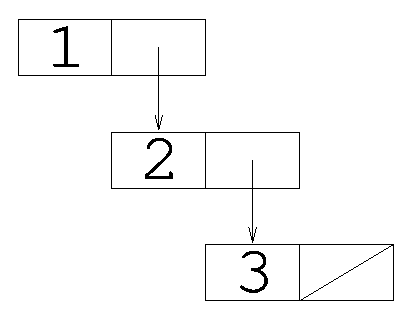
\epsfig{file=cons.ps}}
\end{center}
\end{figure}

List operations are typically implemented in a recursive fashion, where the cdr of the list is taken until the desired element is reached.

\wordtable{
\classword{general-list}{lists}\\
\classword{list}{lists}
}
A \emph{general list} is either the empty list or a cons cell. A \emph{list} is either the empty list or a cons cell whose cdr is also a list. A list is sometimes also known as a \emph{proper list}, and a general list that is not a proper list is known as a \texttt{improper list}. Not all list operations will function given an improper list,
however methods are usually defined on \texttt{general-list} not \texttt{list} since dispatching on \texttt{list} involves a costly check.

\subsubsection{List operations}

\wordtable{
\ordinaryword{>list}{>list ( sequence -- list )}{lists}
}
Turn an arbitrary sequence into a list.
\wordtable{
\ordinaryword{list?}{list?~( obj -- ?~)}{lists}
}
Tests if the object at the top of the stack is a proper list.
\wordtable{
\ordinaryword{unit}{unit ( obj -- [ obj ] )}{lists}
}
Makes a list of one element.
\wordtable{
\ordinaryword{2list}{2list ( o1 o2 -- [ o1 o2 ] )}{lists}
}
Makes a list of two elements.
\wordtable{
\ordinaryword{2unlist}{2unlist ( [ o1 o2 ] -- o1 o2 )}{lists}
}
Pushes the first two elements of a list.
\wordtable{
\ordinaryword{3list}{3list ( o1 o2 o3 -- [ o1 o2 o3 ] )}{lists}
}
Makes a list of three elements.
\wordtable{
\ordinaryword{3unlist}{3unlist ( [ o1 o2 o3 ] -- o1 o2 o3 )}{lists}
}
Pushes the first three elements of a list.
\wordtable{
\ordinaryword{unique}{unique ( obj list -- list )}{lists}
}
If the list already contains an element equal to the object, do nothing, otherwise cons the object into the list.
\wordtable{
\ordinaryword{prune}{prune ( list -- list )}{lists}
}
Removes all duplicates from the list by testing elements for equality.
\wordtable{
\ordinaryword{all=?}{all=?~( list -- ?~)}{lists}
}
Tests if all elements of the list are equal. For the empty list, this is vacuously true.
\wordtable{
\ordinaryword{head}{head~( list n -- list )}{lists}
}
Outputs a new list consisting of the first \texttt{n} elements of \texttt{list}. This allocates memory.
\wordtable{
\ordinaryword{tail}{tail~( list n -- list )}{lists}
}
Outputs a new list consisting of the elements of \texttt{list} from the $n$th index onward. This does not allocate memory; rather it simply takes the \texttt{cdr} \texttt{n} times.
\wordtable{
\ordinaryword{count}{count~( n -- list )}{lists}
}
Return a new list containing all integers from 0 up to $n-1$, inclusive.

\subsubsection{Set-theoretic operations}

\wordtable{
\ordinaryword{contains?}{contains?~( object list -- ?~)}{lists}
}
Tests if \texttt{list} contains an element equal to \texttt{object}.
\wordtable{
\ordinaryword{memq?}{memq?~( object list -- ?~)}{lists}
}
Tests if \texttt{list} contains \texttt{object}. Elements are compared by identity.
\wordtable{
\ordinaryword{contained?}{contained?~( l1 l2 -- ?~)}{lists}
}
Tests if every element of \texttt{l1} is equal to some element of \texttt{l2}.
\wordtable{
\ordinaryword{remove}{remove ( object list -- list )}{lists}
}
Outputs a new list containing all elements of the \texttt{list} except those equal to the \texttt{object}.
\wordtable{
\ordinaryword{remq}{remove ( object list -- list )}{lists}
}
Outputs a new list containing all elements of the \texttt{list} except \texttt{object}. Elements are compared by identity.
\wordtable{
\ordinaryword{intersection}{intersection ( list list -- list )}{lists}
}
Outputs a list of elements present in both lists.
\wordtable{
\ordinaryword{intersection}{difference ( l1 l2 -- list )}{lists}
}
Outputs a list of elements present in \texttt{l2} but not \texttt{l1}.

\subsubsection{List combinators}

\wordtable{
\ordinaryword{each}{each ( list quot -- )}{lists}\\
\texttt{quot:~element --}
}
Applies the quotation to each element of the list.
\wordtable{
\ordinaryword{map}{map ( list quot -- list )}{lists}\\
\texttt{quot:~element -- element}
}
Applies the quotation to each element yielding a new element. The new elements are collected into a new list.
\wordtable{
\ordinaryword{subset}{subset ( list quot -- list )}{lists}\\
\texttt{quot:~element -- ?}
}
Applies the quotation to each element, and outputs a new list containing the elements of the original list for which the quotation output true.
\wordtable{
\ordinaryword{some?}{some?~( list quot -- list )}{lists}\\
\texttt{quot:~element -- ?}
}
Applies the quotation to each element, and outputs the rest of the list upon encountering an element for which the quotation outputs true. If the quotation did not output true for any element, \texttt{some?}~outputs \texttt{f}. Note that the output is a generalized boolean; if the quotation matched any element, the result is true.
\wordtable{
\ordinaryword{all?}{all?~( list quot -- list )}{lists}\\
\texttt{quot:~element -- ?}
}
Outputs \texttt{t} if the quotation yields true when applied to each element, otherwise outputs \texttt{f}. Given the empty list, vacuously outputs \texttt{t}.
\wordtable{
\ordinaryword{sort}{all?~( list quot -- list )}{lists}\\
\texttt{quot:~e1 e2 -- ?}
}
Sorts the list by comparing each pair of elements with the quotation. The quotation should output \texttt{t} if \texttt{e2} is to come before \texttt{e1} in the list. For example, to sort a list of numbers in ascending order, you can do the following:
\begin{alltt}
\textbf{ok} [ 8 6 9 1 10 3 ] [ > ] sort .
[ 1 3 6 8 9 10 ]
\end{alltt}
\wordtable{
\ordinaryword{each-with}{each-with ( object list quot -- )}{lists}\\
\texttt{quot:~object element --}\\
\ordinaryword{map-with}{map-with ( object list quot -- list )}{lists}\\
\texttt{quot:~object element -- element}\\
\ordinaryword{subset-with}{subset-with ( object list quot -- list )}{lists}\\
\texttt{quot:~object element -- ?}\\
\ordinaryword{some-with?}{some-with?~( object list quot -- ?~)}{lists}\\
\texttt{quot:~object element -- ?}\\
\ordinaryword{all-with?}{all-with?~( object list quot -- ?~)}{lists}\\
\texttt{quot:~object element -- ?}
}
Curried forms of the above combinators. They pass an additional object to each invocation of the quotation.

\subsubsection{Queues}

The following set of words manages LIFO (last-in-first-out) queues. Queues are built up from cons cells, and hence are immutable; queue operations always return a new queue.

\wordtable{
\ordinaryword{<queue>}{<queue> ( -- queue )}{lists}
}
Makes a new queue with no elements.
\wordtable{
\ordinaryword{queue-empty?}{queue-empty? ( queue -- ?~)}{lists}
}
Outputs \texttt{t} if the given queue does not contain any elements, \texttt{f} otherwise.
\wordtable{
\ordinaryword{deque}{deque ( queue -- element queue )}{lists}
}
Dequeues an element and outputs a new queue without that element.
\wordtable{
\ordinaryword{enque}{deque ( element queue -- queue )}{lists}
}
Enqueues an element and outputs a new queue.

\subsection{Strings}

\stringglos
\wordtable{
\classword{string}{strings}
}
A string is an immutable sequence of characters. The literal syntax is covered in \ref{string-literals}. Characters do not have a distinct data type, so elements taken out of strings appear as integers on the stack.

\wordtable{
\ordinaryword{string?}{string?~( obj -- ?~)}{strings}
}
Tests if the object at the top of the stack is a string.
%\wordtable{
%\ordinaryword{>string}{>string~( sequence -- string )}{strings}
%}
%Turns any type of sequence with all-integer elements into a string. The integer elements are interpreted as characters.
\wordtable{
\ordinaryword{string-compare}{string-compare~( s1 s2 -- n )}{strings}
}
Compare two strings lexicographically (dictionary order). The output value is one of the following:
\begin{description}
\item[Positive] indicating that \texttt{s1} follows \texttt{s2}
\item[Zero] indicating that \texttt{s1} is equal to \texttt{s2}
\item[Negative] indicating that \texttt{s1} precedes \texttt{s2}
\end{description}
\wordtable{
\ordinaryword{string>}{string> ( s1 s2 -- ?~)}{strings}
}
Tests if \texttt{s1} follows \texttt{s2}. Implemented as follows:
\begin{verbatim}
: string> ( s1 s1 -- ? ) string-compare 0 > ;
\end{verbatim}
This is used to sort lists of strings:
\begin{alltt}
\textbf{ok} [ "Curry" "Apple" "Veal" "Turkey" ] [ string> ] sort .
[ "Apple" "Curry" "Turkey" "Veal" ]
\end{alltt}
\wordtable{
\ordinaryword{fill}{fill~( n char -- string )}{strings}
}
Creates a string with \texttt{char} repeated $n$ times.
\wordtable{
\ordinaryword{pad}{pad~( string n char -- string )}{strings}
}
Creates a string with \texttt{char} repeated $l-n$ times, where $l$ is the length of \texttt{string}. If $l$ is greater than $n$, the empty string is output.

\subsubsection{Substring testing}

\wordtable{
\ordinaryword{string-contains?}{string-contains?~( s1 s2 -- ?~)}{strings}
}
Tests if \texttt{s2} contains \texttt{s1} as a substring.
\wordtable{
\ordinaryword{string-head?}{string-head?~( s1 s2 -- ?~)}{strings}\\
\ordinaryword{string-tail?}{string-tail?~( s1 s2 -- ?~)}{strings}
}
Tests if \texttt{s1} starts or ends with \texttt{s1} as a substring. If \texttt{s1} is longer than \texttt{s2}, outputs \texttt{f}.

\subsubsection{Slicing and splitting}

\wordtable{
\ordinaryword{string/}{string/ ( string n -- s1 s2 )}{strings}
}
Outputs a pair of strings that equal the original string when concatenated. The first string has length $n$, the second has length $l-n$ where $l$ is the length of the input.
\begin{alltt}
\textbf{ok} "Hello world" 5 string .s
\textbf{" world"
"Hello"}
\end{alltt}
\wordtable{
\ordinaryword{string//}{string// ( string n -- s1 s2 )}{strings}
}

Outputs a pair of strings that equal the original string, excluding the $n$th element, when concatenated. The first string has length $n$, the second has length $l-n$ where $l$ is the length of the input.
\begin{alltt}
\textbf{ok} "Hello world" 5 string// .s
\textbf{"world"
"Hello"}
\end{alltt}
\wordtable{
\ordinaryword{?string-head}{?string-head~( s1 s2 -- string ?~)}{strings}\\
\ordinaryword{?string-tail}{?string-tail~( s1 s2 -- string ?~)}{strings}
}
Tests if \texttt{s1} starts or ends with \texttt{s1} as a substring. If there is a match, outputs the subrange of \texttt{s1} excluding \texttt{s1} followed by \texttt{t}. If there is no match, outputs \texttt{s1} followed by \texttt{f}/
\wordtable{
\ordinaryword{split1}{split1~( str split -- before after )}{strings}
}
If \texttt{string} does not contain \texttt{split} as a substring, then \texttt{before} is equal to the \texttt{string}, and \texttt{after} is \texttt{f}. Otherwise, \texttt{before} and \texttt{after} are both strings, and yield the input excluding \texttt{split} when concatenated.
\wordtable{
\ordinaryword{split}{split~( str split -- list )}{strings}
}
Outputs a list of substrings taken between occurrences of \texttt{split} in \texttt{string}. If \texttt{split} does not occur inside \texttt{string}, outputs a singleton list containing \texttt{string} only.
\begin{alltt}
\textbf{ok} "/usr/local/bin" CHAR: / split .
\textbf{[ "" "usr" "local" "bin" ]}
\end{alltt}
\wordtable{
\ordinaryword{split-n}{split-n~( str n -- list )}{strings}
}
Splits the string into groups of \texttt{n} characters and collects them in a list. If the string's length is not a multiple of \texttt{n}, the final string in the list might be shorter.

\subsubsection{Characters}

\wordtable{
\ordinaryword{ch>string}{ch>string ( n -- string )}{strings}
}
Turns an integer representing a character value into a single-element string.
\wordtable{
\ordinaryword{blank?}{blank?~( n -- ?~)}{strings}\\
\ordinaryword{letter?}{letter?~( n -- ?~)}{strings}\\
\ordinaryword{LETTER?}{LETTER?~( n -- ?~)}{strings}\\
\ordinaryword{digit?}{digit?~( n -- ?~)}{strings}\\
\ordinaryword{printable?}{printable?~( n -- ?~)}{strings}\\
\ordinaryword{quotable?}{quotable?~( n -- ?~)}{strings}\\
\ordinaryword{url-quotable?}{url-quotable?~( n -- ?~)}{strings}
}
Various character classification predicates.

\subsection{String buffers}

\sbufglos
\wordtable{
\classword{sbuf}{strings}
}
A string buffer is a mutable and growable sequence of characters. String buffers can be used to construct new strings by accumilating substrings and characters, however usually they are only used indirectly, since the sequence construction words in \ref{make-seq} are more convenient to use in many cases.
\wordtable{
\ordinaryword{sbuf?}{sbuf?~( object -- ?~)}{strings}
}
Tests if the object at the top of the stack is a string buffer.
\wordtable{
\ordinaryword{>sbuf}{>sbuf~( sequence -- sbuf )}{strings}
}
Turns any type of sequence into a string buffer. Given a string buffer, this makes a fresh copy
\wordtable{
\ordinaryword{sbuf>string}{sbuf>string~( sbuf -- string )}{strings}
}
Turns a string buffer into a string holding the same characters.

\subsection{\label{make-seq}Constructing sequences}

The library supports an idiom where sequences can be constructed without passing the partial sequence being built on the stack. This reduces stack noise, and thus simplifies code and makes it easier to understand.

\newcommand{\dynamicscopeglos}{\glossary{
name=dynamic scope,
description={a variable binding policy where bindings established in a scope are visible to all code executed while the scope is active}}}
\dynamicscopeglos
\wordtable{
\ordinaryword{make-list}{make-list ( quot -- list )}{namespaces}\\
\ordinaryword{make-string}{make-string ( quot -- string )}{namespaces}\\
\ordinaryword{make-sbuf}{make-sbuf ( quot -- string )}{namespaces}\\
\ordinaryword{make-vector}{make-vector ( quot -- vector )}{namespaces}
}
Calls the quotation in a new \texttt{dynamic scope}. The quotation and any words it calls can execute the \texttt{,} and \texttt{\%} words to add elements at the end of the sequence being constructed.
\wordtable{
\ordinaryword{,}{,~( element -- )}{namespaces}
}
Adds the element to the end of the sequence being constructed by the innermost call to one of the above combinators.
\wordtable{
\ordinaryword{unique,}{unique,~( element -- )}{namespaces}
}
Adds the element to the end of the sequence being constructed as long as the sequence does not already have an equal element.
\wordtable{
\ordinaryword{literal,}{literal,~( element -- )}{namespaces}
}
Adds the element wrapped inside a one-element list, then adds the \texttt{car} word. This is used to construct quotations with \texttt{make-list} that must push a word on the stack.
\wordtable{
\ordinaryword{\%}{\% ( sequence -- )}{namespaces}
}
Appends the subsequence to the end of the sequence being constructed.

Note that the sequence construction combinators will capture any variables set inside the quotation, due to the dynamic scoping behavior. These combinators are actually implemented using variables. See \ref{namespaces}.

\section{Mappings}

\glossary{name=mapping,
description={an unordered collection of elements, accessed by key. Examples include association lists and hashtables}}

Mappings associate keys with values. The two classes of mappings in the Factor library are association lists and hashtables.

\begin{tabular}[t]{l|c|c|c|l}
Class&Mutable&Ordered&Lookup&Primary purpose\\
\hline
\texttt{assoc}&&$\surd$&$O(n)$&Small, unchanging mappings\\
\texttt{hashtable}&$\surd$&&$O(1)$&Large or frequently-changing mappings
\end{tabular}

It might be tempting to just always use hashtables, however for very small mappings, association lists are just as efficient, and are easier to work with since the entire set of list words can be used with them.

\subsection{Association lists}

\glossary{name=association list,
description={a list of pairs, where the car if each pair is a key and the cdr is the value associated with that key}}

Association lists are built from cons cells. They are structured like a ribbed spine, where the ``spine'' is a list and each ``rib'' is a cons cell holding a key/value pair.

\wordtable{
\ordinaryword{assoc?}{assoc ( object -- ?~)}{lists}
}
Tests if the object at the top of the stack is a proper list whose every element is a cons.

\wordtable{
\ordinaryword{assoc}{assoc ( k alist -- v )}{lists}\\
\ordinaryword{assoc*}{assoc* ( k alist -- [[ k v ]] )}{lists}
}
These words look up a key in an association list, comparing keys in the list with the given key by equality with \texttt{=}. The list is searched starting from the beginning. The two words differ in that the latter returns the key/value pair located, whereas the former only returns the value. The \texttt{assoc*} word allows a distinction to be made between a missing value and a value equal to \texttt{f}, since in the case of a missing value it outputs \texttt{f}.
\wordtable{
\ordinaryword{assq}{assq ( k alist -- v )}{lists}\\
\ordinaryword{assq*}{assq* ( k alist -- [[ k v ]] )}{lists}
}
These words compare keys by identity with \texttt{eq?}~and are dual to \texttt{assoc} and \texttt{assoc*}.
\wordtable{
\ordinaryword{acons}{acons ( v k alist -- alist )}{lists}\\
\ordinaryword{set-assoc}{set-assoc ( v k alist -- alist )}{lists}
}
These words output a new association list containing the key/value pair.
They differ in that \texttt{set-assoc} removes any existing key/value pairs with the given key first. In both cases, searching for the key in the returned association list gives the new value, however with the slightly faster \texttt{acons}, the old value remains shadowed in the list.
\wordtable{
\ordinaryword{remove-assoc}{remove-assoc ( k alist -- alist )}{lists}
}
Outputs a new association list which does not have any key/value pairs with the key equal to \texttt{k}.

\begin{figure}
\caption{An association list and its graphical representation}
\begin{verbatim}
[
    [[ "Salsa" "Hot" ]]
    [[ "Stir-Fry" "Medium" ]]
    [[ "Peppers" "Very Hot" ]]
]
\end{verbatim}

\begin{center}
\scalebox{0.45}{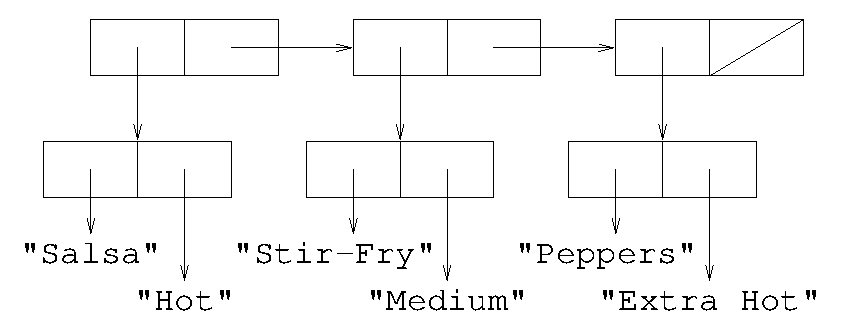
\epsfig{file=assoc.eps}}
\end{center}
\end{figure}

\subsubsection{Dual representation}

Sometimes it is convenient to decompose an association list into two lists of equal length, containing the keys and values, respectively, in the same order as the association list. This dual representation can be manipulated with a handful of helper words.

\wordtable{
\ordinaryword{zip}{zip ( keys values -- alist )}{lists}\\
\ordinaryword{unzip}{unzip ( alist -- keys values )}{lists}
}
These words convert between pairs of lists and lists of pairs.
\begin{alltt}
\textbf{ok} [ 1 2 3 ] [ 4 5 6 ] zip .
[ [[ 1 4 ]] [[ 2 5 ]] [[ 3 6 ]] ]
\textbf{ok} [ [[ 1 2 ]] [[ 3 4 ]] [[ 5 6 ]] ] unzip .s
[ 2 4 6 ]
[ 1 3 5 ]
\end{alltt}
\wordtable{
\ordinaryword{2cons}{2cons ( car1 car2 cdr1 cdr2 -- c1 c2 )}{lists}
}
Cons a pair of elements onto a pair of lists.
\wordtable{
\ordinaryword{2car}{2car ( c1 c2 -- car1 car2 )}{lists}\\
\ordinaryword{2cdr}{2cdr ( c1 c2 -- cdr1 cdr2 )}{lists}
}
Deconstructs paired lists.

\subsection{Hashtables}

\wordtable{
\classword{hashtable}{hashtables}
}


\subsection{\label{namespaces}Namespaces}

\section{Mathematics}

\numberglos

\begin{figure}
\begin{center}
\caption{Numerical class hierarchy}
\scalebox{0.5}{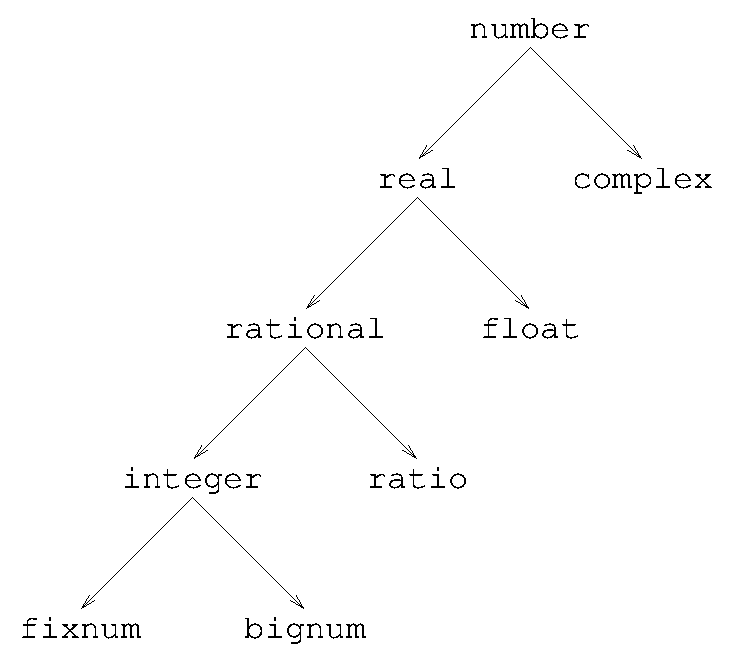
\epsfig{file=number.ps}}
\end{center}
\end{figure}

Factor's numbers more closely model the mathematical concept of a number than other languages. Where possible, exact answers are given -- for example, adding or multiplying two integers never results in overflow, and dividing two integers yields a fraction rather than a truncated result. Complex numbers are supported, allowing many functions to be computed with parameters that would raise errors or return ``not a number'' in other languages.

\subsection{Integers}

\integerglos

The simplest type of number is the integer. Integers come in two varieties -- \emph{fixnums} and \emph{bignums}. As their names suggest, a fixnum is a fixed-width quantity\footnote{Fixnums range in size from $-2^{w-3}-1$ to $2^{w-3}$, where $w$ is the word size of your processor (for example, 32 bits). Because fixnums automatically grow to bignums, usually you do not have to worry about details like this.}, and is a bit quicker to manipulate than an arbitrary-precision bignum.

The predicate word \texttt{integer?}~tests if the top of the stack is an integer. If this returns true, then exactly one of \texttt{fixnum?}~or \texttt{bignum?}~would return true for that object. Usually, your code does not have to worry if it is dealing with fixnums or bignums.

Unlike some languages where the programmer has to declare storage size explicitly and worry about overflow, integer operations automatically return bignums if the result would be too big to fit in a fixnum. Here is an example where multiplying two fixnums returns a bignum:

\begin{alltt}
\textbf{ok} 134217728 fixnum? .
\textbf{t}
\textbf{ok} 128 fixnum? .
\textbf{t}
\textbf{ok} 134217728 128 * .
\textbf{17179869184}
\textbf{ok} 134217728 128 * bignum? .
\textbf{t}
\end{alltt}

Integers can be entered using a different base. By default, all number entry is in base 10, however this can be changed by prefixing integer literals with one of the parsing words \texttt{BIN:}, \texttt{OCT:}, or \texttt{HEX:}. For example:

\begin{alltt}
\textbf{ok} BIN: 1110 BIN: 1 + .
\textbf{15}
\textbf{ok} HEX: deadbeef 2 * .
\textbf{7471857118}
\end{alltt}

The word \texttt{.} prints numbers in decimal, regardless of how they were input. A set of words in the \texttt{prettyprint} vocabulary is provided for print integers using another base.

\begin{alltt}
\textbf{ok} 1234 .h
\textbf{4d2}
\textbf{ok} 1234 .o
\textbf{2232}
\textbf{ok} 1234 .b
\textbf{10011010010}
\end{alltt}

\subsection{Rational numbers}

\newcommand{\rationalglos}{\glossary{
name=rational,
description={an instance of the \texttt{rational} class, which is a disjoint union of the
\texttt{integer} and \texttt{ratio} classes}}}
\rationalglos
\ratioglos

If we add, subtract or multiply any two integers, the result is always an integer. However, this is not the case with division. When dividing a numerator by a denominator where the numerator is not a integer multiple of the denominator, a ratio is returned instead.

\begin{alltt}
1210 11 / .
\emph{110}
100 330 / .
\emph{10/33}
\end{alltt}

Ratios are printed and can be input literally in the form of the second example. Ratios are always reduced to lowest terms by factoring out the greatest common divisor of the numerator and denominator. A ratio with a denominator of 1 becomes an integer. Trying to create a ratio with a denominator of 0 raises an error.

The predicate word \texttt{ratio?}~tests if the top of the stack is a ratio. The predicate word \texttt{rational?}~returns true if and only if one of \texttt{integer?}~or \texttt{ratio?}~would return true for that object. So in Factor terms, a ``ratio'' is a rational number whose denominator is not equal to 1.

Ratios behave just like any other number -- all numerical operations work as expected, and in fact they use the formulas for adding, subtracting and multiplying fractions that you learned in high school.

\begin{alltt}
\textbf{ok} 1/2 1/3 + .
\textbf{5/6}
\textbf{ok} 100 6 / 3 * .
\textbf{50}
\end{alltt}

Ratios can be deconstructed into their numerator and denominator components using the \texttt{numerator} and \texttt{denominator} words. The numerator and denominator are both integers, and furthermore the denominator is always positive. When applied to integers, the numerator is the integer itself, and the denominator is 1.

\begin{alltt}
\textbf{ok} 75/33 numerator .
\textbf{25}
\textbf{ok} 75/33 denominator .
\textbf{11}
\textbf{ok} 12 numerator .
\textbf{12}
\end{alltt}

\subsection{Floating point numbers}

\newcommand{\realglos}{\glossary{
name=real,
description={an instance of the \texttt{real} class, which is a disjoint union of the
\texttt{rational} and \texttt{float} classes}}}
\realglos
\floatglos

Rational numbers represent \emph{exact} quantities. On the other hand, a floating point number is an \emph{approximation}. While rationals can grow to any required precision, floating point numbers are fixed-width, and manipulating them is usually faster than manipulating ratios or bignums (but slower than manipulating fixnums). Floating point literals are often used to represent irrational numbers, which have no exact representation as a ratio of two integers. Floating point literals are input with a decimal point.

\begin{alltt}
\textbf{ok} 1.23 1.5 + .
\textbf{1.73}
\end{alltt}

The predicate word \texttt{float?}~tests if the top of the stack is a floating point number. The predicate word \texttt{real?}~returns true if and only if one of \texttt{rational?}~or \texttt{float?}~would return true for that object.

Floating point numbers are \emph{contagious} -- introducing a floating point number in a computation ensures the result is also floating point.

\begin{alltt}
\textbf{ok} 5/4 1/2 + .
\textbf{7/4}
\textbf{ok} 5/4 0.5 + .
\textbf{1.75}
\end{alltt}

Apart from contaigion, there are two ways of obtaining a floating point result from a computation; the word \texttt{>float ( n -{}- f )} converts a rational number into its floating point approximation, and the word \texttt{/f ( x y -{}- x/y )} returns the floating point approximation of a quotient of two numbers.

\begin{alltt}
\textbf{ok} 7 4 / >float .
\textbf{1.75}
\textbf{ok} 7 4 /f .
\textbf{1.75}
\end{alltt}

Indeed, the word \texttt{/f} could be defined as follows:

\begin{alltt}
: /f / >float ;
\end{alltt}

However, the actual definition is slightly more efficient, since it computes the floating point result directly.

\subsection{Complex numbers}

Complex numbers arise as solutions to quadratic equations whose graph does not intersect the x axis. For example, the equation $x^2 + 1 = 0$ has no solution for real $x$, because there is no real number that is a square root of -1. However, in the field of complex numbers, this equation has a well-known solution:

\begin{alltt}
\textbf{ok} -1 sqrt .
\textbf{\#\{ 0 1 \}}
\end{alltt}

The literal syntax for a complex number is \texttt{\#\{ re im \}}, where \texttt{re} is the real part and \texttt{im} is the imaginary part. For example, the literal \texttt{\#\{ 1/2 1/3 \}} corresponds to the complex number $1/2 + 1/3i$.

The words \texttt{i} an \texttt{-i} push the literals \texttt{\#\{ 0 1 \}} and \texttt{\#\{ 0 -1 \}}, respectively.

The predicate word \texttt{complex?} tests if the top of the stack is a complex number. Note that unlike math, where all real numbers are also complex numbers, Factor only considers a number to be a complex number if its imaginary part is non-zero.

Complex numbers can be deconstructed into their real and imaginary components using the \texttt{real} and \texttt{imaginary} words. Both components can be pushed at once using the word \texttt{>rect ( z -{}- re im )}.

\begin{alltt}
\textbf{ok} -1 sqrt real .
\textbf{0}
\textbf{ok} -1 sqrt imaginary .
\textbf{1}
\textbf{ok} -1 sqrt sqrt >rect .s
\textbf{\{ 0.7071067811865476 0.7071067811865475 \}}
\end{alltt}

A complex number can be constructed from a real and imaginary component on the stack using the word \texttt{rect> ( re im -{}- z )}.

\begin{alltt}
\textbf{ok} 1/3 5 rect> .
\textbf{\#\{ 1/3 5 \}}
\end{alltt}

Complex numbers are stored in \emph{rectangular form} as a real/imaginary component pair (this is where the names \texttt{>rect} and \texttt{rect>} come from). An alternative complex number representation is \emph{polar form}, consisting of an absolute value and argument. The absolute value and argument can be computed using the words \texttt{abs} and \texttt{arg}, and both can be pushed at once using \texttt{>polar ( z -{}- abs arg )}.

\begin{alltt}
\textbf{ok} 5.3 abs .
\textbf{5.3}
\textbf{ok} i arg .
\textbf{1.570796326794897}
\textbf{ok} \#\{ 4 5 \} >polar .s
\textbf{\{ 6.403124237432849 0.8960553845713439 \}}
\end{alltt}

A new complex number can be created from an absolute value and argument using \texttt{polar> ( abs arg -{}- z )}.

\begin{alltt}
\textbf{ok} 1 pi polar> .
\textbf{\#\{ -1.0 1.224606353822377e-16 \}}
\end{alltt}

\subsection{Transcedential functions}

The \texttt{math} vocabulary provides a rich library of mathematical functions that covers exponentiation, logarithms, trigonometry, and hyperbolic functions. All functions accept and return complex number arguments where appropriate. These functions all return floating point values, or complex numbers whose real and imaginary components are floating point values.

\texttt{\^{} ( x y -- x\^{}y )} raises \texttt{x} to the power of \texttt{y}. In the cases of \texttt{y} being equal to $1/2$, -1, or 2, respectively, the words \texttt{sqrt}, \texttt{recip} and \texttt{sq} can be used instead.

\begin{alltt}
\textbf{ok} 2 4 \^ .
\textbf{16.0}
\textbf{ok} i i \^ .
\textbf{0.2078795763507619}
\end{alltt}

All remaining functions have a stack effect \texttt{( x -{}- y )}, it won't be repeated for brevity.

\texttt{exp} raises the number $e$ to a specified power. The number $e$ can be pushed on the stack with the \texttt{e} word, so \texttt{exp} could have been defined as follows:

\begin{alltt}
: exp ( x -- e^x ) e swap \^ ;
\end{alltt}

However, it is actually defined otherwise, for efficiency.\footnote{In fact, the word \texttt{\^{}} is actually defined in terms of \texttt{exp}, to correctly handle complex number arguments.}

\texttt{log} computes the natural (base $e$) logarithm. This is the inverse of the \texttt{exp} function.

\begin{alltt}
\textbf{ok} -1 log .
\textbf{\#\{ 0.0 3.141592653589793 \}}
\textbf{ok} e log .
\textbf{1.0}
\end{alltt}

\texttt{sin}, \texttt{cos} and \texttt{tan} are the familiar trigonometric functions, and \texttt{asin}, \texttt{acos} and \texttt{atan} are their inverses.

The reciprocals of the sine, cosine and tangent are defined as \texttt{sec}, \texttt{cosec} and \texttt{cot}, respectively. Their inverses are \texttt{asec}, \texttt{acosec} and \texttt{acot}.

\texttt{sinh}, \texttt{cosh} and \texttt{tanh} are the hyperbolic functions, and \texttt{asinh}, \texttt{acosh} and \texttt{atanh} are their inverses.

Similarly, the reciprocals of the hyperbolic functions are defined as \texttt{sech}, \texttt{cosech} and \texttt{coth}, respectively. Their inverses are \texttt{asech}, \texttt{acosech} and \texttt{acoth}.

\subsection{Modular arithmetic}

In addition to the standard division operator \texttt{/}, there are a few related functions that are useful when working with integers.

\texttt{/i ( x y -{}- x/y )} performs a truncating integer division. It could have been defined as follows:

\begin{alltt}
: /i / >integer ;
\end{alltt}

However, the actual definition is a bit more efficient than that.

\texttt{mod ( x y -{}- x\%y )} computes the remainder of dividing \texttt{x} by \texttt{y}. If the result is 0, then \texttt{x} is a multiple of \texttt{y}.

\texttt{/mod ( x y -{}- x/y x\%y )} pushes both the quotient and remainder.

\begin{alltt}
\textbf{ok} 100 3 mod .
\textbf{1}
\textbf{ok} -546 34 mod .
\textbf{-2}
\end{alltt}

\texttt{gcd ( x y -{}- z )} pushes the greatest common divisor of two integers; that is, the largest number that both integers could be divided by and still yield integers as results. This word is used behind the scenes to reduce rational numbers to lowest terms when doing ratio arithmetic.

\subsection{Bitwise operations}

There are two ways of looking at an integer -- as a mathematical entity, or as a string of bits. The latter representation faciliates the so-called \emph{bitwise operations}.

\texttt{bitand ( x y -{}- x\&y )} returns a new integer where each bit is set if and only if the corresponding bit is set in both $x$ and $y$. If you're considering an integer as a sequence of bit flags, taking the bitwise-and with a mask switches off all flags that are not explicitly set in the mask.

\begin{alltt}
BIN: 101 BIN: 10 bitand .b
\emph{0}
BIN: 110 BIN: 10 bitand .b
\emph{10}
\end{alltt}

\texttt{bitor ( x y -{}- x|y )} returns a new integer where each bit is set if and only if the corresponding bit is set in at least one of $x$ or $y$. If you're considering an integer as a sequence of bit flags, taking the bitwise-or with a mask switches on all flags that are set in the mask.

\begin{alltt}
BIN: 101 BIN: 10 bitor .b
\emph{111}
BIN: 110 BIN: 10 bitor .b
\emph{110}
\end{alltt}

\texttt{bitxor ( x y -{}- x\^{}y )} returns a new integer where each bit is set if and only if the corresponding bit is set in exactly one of $x$ or $y$. If you're considering an integer as a sequence of bit flags, taking the bitwise-xor with a mask toggles on all flags that are set in the mask.

\begin{alltt}
BIN: 101 BIN: 10 bitxor .b
\emph{111}
BIN: 110 BIN: 10 bitxor .b
\emph{100}
\end{alltt}

\texttt{bitnot ( x -{}- y )} returns the bitwise complement of the input; that is, each bit in the input number is flipped. This is actually equivalent to negating a number, and subtracting one. So indeed, \texttt{bitnot} could have been defined as thus:

\begin{alltt}
: bitnot neg pred ;
\end{alltt}

\texttt{shift ( x n -{}- y )} returns a new integer consisting of the bits of the first integer, shifted to the left by $n$ positions. If $n$ is negative, the bits are shifted to the right instead, and bits that ``fall off'' are discarded.

\begin{alltt}
BIN: 101 5 shift .b
\emph{10100000}
BIN: 11111 -2 shift .b
\emph{111}
\end{alltt}

The attentive reader will notice that shifting to the left is equivalent to multiplying by a power of two, and shifting to the right is equivalent to performing a truncating division by a power of two.

\chapter{The development environment}

Factor supports interactive development in a live environment. Instead of working with
static executable files and restarting your application after each change, you can
incrementally make changes to your application and test them immediately. If you
notice an undesirable behavior, Factor's powerful reflection features will aid in
pinpointing the error.

If you are used to a statically typed language, you might find Factor's tendency to only fail at runtime hard to work with at first. However, the interactive development tools outlined in this document allow a much quicker turn-around time for testing changes. Also, write unit tests -- unit testing is a great way to ensure that old bugs do not re-appear once they've been fixed.

\section{System organization}

\subsection{The listener}

Factor is an \emph{image-based environment}. When you compiled Factor, you also generated a file named \texttt{factor.image}. I will have more to say about images later, but for now it suffices to understand that to start Factor, you must pass the image file name on the command line:
\begin{alltt}
./f factor.image
\textbf{Loading factor.image... relocating... done
Factor 0.73 :: http://factor.sourceforge.net :: unix/x86
(C) 2003, 2005 Slava Pestov, Chris Double,
Mackenzie Straight
ok}
\end{alltt}
An \texttt{\textbf{ok}} prompt is printed after the initial banner, indicating the listener is ready to execute Factor phrases. The listener is a piece of Factor code, like any other; however, it helps to think of it as the primary interface to the Factor system. The listener reads Factor code and executes it. You can try the classical first program:

\begin{alltt}
\textbf{ok} "Hello, world." print
\textbf{Hello, world.}
\end{alltt}


Multi-line phrases are supported; if there are unclosed brackets, the listener outputs \texttt{...} instead of the \texttt{ok} prompt, and the entire phrase is executed once all brackets are closed:

\begin{alltt}
\textbf{ok} [ 1 2 3 ] [
\textbf{...} .
\textbf{...} ] each
\textbf{1
2
3}
\end{alltt}

The listener knows when to print a continuation prompt by looking at the height of the
stack. Parsing words such as \texttt{[} and \texttt{:} leave elements on the parser
stack; these elements are popped by \texttt{]} and \texttt{;}.

\subsection{Source files}

While it is possible to do all development in the listener and save your work in images, it is far more convenient to work with source files, at least until an in-image structure editor is developed.

By convention, Factor source files are saved with the \texttt{.factor} filename extension. They can be loaded into the image as follows:

\begin{alltt}
\textbf{ok} "examples/numbers-game.factor" run-file
\end{alltt}

In Factor, loading a source file replaces any existing definitions\footnote{But see \ref{compiler} for this is not true of compiled code.}. Each word definition remembers what source file it was loaded from (if any). To reload the source file associated with a definition, use the \texttt{reload} word:

\begin{alltt}
\textbf{ok} \bs draw reload
\end{alltt}

Word definitions also retain the line number where they are located in their original source file. This allows you to open a word definition in jEdit\footnote{\texttt{http://www.jedit.org}} for editing using the
\texttt{jedit} word:

\begin{alltt}
\textbf{ok} \bs compile jedit
\end{alltt}

This word requires that a jEdit instance is already running.

For the \texttt{jedit} word to work with words in the Factor library, you must set the \texttt{"resource-path"} variable to the location of the Factor source tree. One way to do this is to add a phrase like the following to your \texttt{.factor-rc}:

\begin{verbatim}
"/home/slava/Factor/" "resource-path" set
\end{verbatim}

On startup, Factor reads the \texttt{.factor-rc} file from your home directory. You can put
any quick definitions you want available at the listener there. To avoid loading this
file, pass the \texttt{-no-user-init} command line switch. Another way to have a set of definitions available at all times is to save a custom image, as described in the next section.

\subsection{Images}

The \texttt{factor.image} file is basically a dump of all objects in the heap. A new image can be saved as follows:

\begin{alltt}
\textbf{ok} "work.image" save-image
\textbf{Saving work.image...}
\end{alltt}

When you save an image before exiting Factor, then start Factor again, everything will be almost as you left it. Try the following:

\begin{alltt}
./f factor.image
\textbf{ok} "Learn Factor" "reminder" set
\textbf{ok} "factor.image" save-image bye
\textbf{Saving factor.image...}
\end{alltt}

Factor will save the image and exit. Now start it again and see that the reminder is still there:

\begin{alltt}
./f factor.image
\textbf{ok} "reminder" get .
\textbf{"Learn Factor"}
\end{alltt}

This is what is meant by the image being an \emph{infinite session}. When you shut down and restart Factor, what happends is much closer to a Laptop's ``suspend'' mode, than a desktop computer being fully shut down.

\subsection{Looking at objects}

Probably the most important debugging tool of them all is the \texttt{.} word. It prints the object at the top of the stack in a form that can be parsed by the Factor parser. A related word is \texttt{prettyprint}. It is identical to \texttt{.} except the output is more verbose; lists, vectors and hashtables are broken up into multiple lines and indented.

\begin{alltt}
\textbf{ok} [ [ \tto 1 \ttc \tto 2 \ttc ] dup car swap cdr ] .
[ [ \tto 1 \ttc \tto 2 \ttc ] dup car swap cdr ]
\end{alltt}

Most objects print in a parsable form, but not all. One exceptions to this rule is objects with external state, such as I/O ports or aliens (pointers to native structures). Also, objects with circular or very deeply nested structure will not print in a fully parsable form, since the prettyprinter has a limit on maximum nesting. Here is an example -- a vector is created, that holds a list whose first element is the vector itself:

\begin{alltt}
\textbf{ok} \tto \ttc [ unit 0 ] keep [ set-vector-nth ] keep .
\tto [ ... ] \ttc
\end{alltt}

The prettyprinted form of a vector or list with many elements is not always readable. The \texttt{[.]} and \texttt{\tto.\ttc} words output a list or a vector, respectively, with each element on its own line. In fact, the stack printing words are defined in terms of \texttt{[.]} and \texttt{\tto.\ttc}:

\begin{verbatim}
: .s datastack  {.} ;
: .r callstack  {.} ;
: .n namestack  [.] ;
: .c catchstack [.] ;
\end{verbatim}

Before we move on, one final set of output words comes is used to output integers in
different numeric bases. The \texttt{.b} word prints an integer in binary, \texttt{.o} in octal, and \texttt{.h} in hexadecimal.

\begin{alltt}
\textbf{ok} 31337 .b
\textbf{111101001101001}
\textbf{ok} 31337 .o
\textbf{75151}
\textbf{ok} 31337 .h
\textbf{7a69}
\end{alltt}

\section{Word tools}

\subsection{Exploring vocabularies}

Factor organizes code in a two-tier structure of vocabularies and words. A word is the smallest unit of code; it corresponds to a function or method in other languages. Vocabularies group related words together for easy browsing and tracking of source dependencies.

Entering \texttt{vocabs .}~in the listener produces a list of all existing vocabularies:

\begin{alltt}
\textbf{ok} vocabs .
\textbf{[ "alien" "ansi" "assembler" "browser-responder"
"command-line" "compiler" "cont-responder" "errors"
"file-responder" "files" "gadgets" "generic"
"hashtables" "html" "httpd" "httpd-responder" "image"
"inference" "interpreter" "io-internals" "jedit"
"kernel" "kernel-internals" "line-editor" "listener"
"lists" "logging" "math" "math-internals" "memory"
"namespaces" "parser" "prettyprint" "profiler"
"quit-responder" "random" "resource-responder"
"scratchpad" "sdl" "shells" "stdio" "streams"
"strings" "syntax" "telnetd" "test" "test-responder"
"threads" "unparser" "url-encoding" "vectors" "words" ]}
\end{alltt}

As you can see, there are a lot of vocabularies! Now, you can use \texttt{words .}~to list the words inside a given vocabulary:

\begin{alltt}
\textbf{ok} "namespaces" words .
\textbf{[ (get) , <namespace> >n append, bind change cons@
dec extend get global inc init-namespaces list-buffer
literal, make-list make-rlist make-rstring make-string
make-vector n> namespace namestack nest off on put set
set-global set-namestack unique, unique@ with-scope ]}
\end{alltt}

You can look at the definition of any word, including library words, using \texttt{see}. Keep in mind you might have to \texttt{USE:} the vocabulary first.

\begin{alltt}
\textbf{ok} USE: httpd
\textbf{ok} \bs httpd-connection see
\textbf{IN: httpd : httpd-connection ( socket -- )
    "http-server" get accept [
        httpd-client
    ] in-thread drop ;}
\end{alltt}

The \texttt{see} word shows a reconstruction of the source code, not the original source code. So in particular, formatting and some comments are lost.

\subsection{Cross-referencing words}

The \texttt{apropos.} word is handy when searching for related words. It lists all words
whose names contain a given string. The \texttt{apropos.} word is also useful when you know the exact name of a word, but are unsure what vocabulary it is in. For example, if you're looking for ways to iterate over various collections, you can do an apropos search for \texttt{map}:

\begin{alltt}
\textbf{ok} "map" apropos.
\textbf{IN: inference
type-value-map
IN: lists
map
map-with
IN: sdl
set-surface-map
surface-map
IN: strings
string-map
IN: vectors
vector-map}
\end{alltt}

From the above output, you can see that \texttt{map} is for lists, \texttt{string-map} is for strings, and \texttt{vector-map} is for vectors.

The \texttt{usage} word finds all words that refer to a given word and pushes a list on the stack. This word is helpful in two situations; the first is for learning -- a good way to learn a word is to see it used in context. The second is during refactoring -- if you change a word's stack effect, you must also update all words that call it. Usually you print the
return value of \texttt{usage} using \texttt{.}:

\begin{alltt}
\textbf{ok} \bs string-map usage .
\textbf{schars>entities
filter-null
url-encode}
\end{alltt}

Another useful word is \texttt{usages}. Unlike \texttt{usage}, it finds all usages, even
indirect ones -- so if a word refers to another word that refers to the given word,
both words will be in the output list.

\subsection{Exploring classes}

Factor supports object-oriented programming via generic words. Generic words are called
like ordinary words, however they can have multiple definitions, one per class, and
these definitions do not have to appear in the same source file. Such a definition is
termed a \emph{method}, and the method is said to \emph{specialize} on a certain
class. A class in the most
general sense is just a set of objects. You can output a list of classes in the system
with \texttt{classes .}:

\begin{alltt}
\textbf{ok} classes.
\textbf{[ alien alien-error byte-array displaced-alien
dll ansi-stream disp-only displaced indirect operand
register absolute absolute-16/16 relative relative-bitfld
item kernel-error no-method border checkbox dialog editor
ellipse etched-rect frame gadget hand hollow-ellipse
hollow-rect label line menu pane pile plain-ellipse
plain-rect rectangle roll-rect scroller shelf slider
stack tile viewport world 2generic arrayed builtin
complement generic null object predicate tuple
tuple-class union hashtable html-stream class-tie
computed inference-error inference-warning literal
literal-tie value buffer port jedit-stream boolean
general-t array cons general-list list bignum complex
fixnum float integer number ratio rational real
parse-error potential-float potential-ratio
button-down-event button-up-event joy-axis-event
joy-ball-event joy-button-down-event joy-button-up-event
joy-hat-event key-down-event key-up-event motion-event
quit-event resize-event user-event sequence stdio-stream
client-stream fd-stream null-stream server string-output
wrapper-stream LETTER blank digit letter printable sbuf
string text POSTPONE: f POSTPONE: t vector compound
primitive symbol undefined word ]}
\end{alltt}

If you \texttt{see} a generic word, all methods defined on the generic word are shown.
Alternatively, you can use \texttt{methods.} to print all methods specializing on a
given class:

\begin{alltt}
\textbf{ok} \bs list methods.
\textbf{PREDICATE: general-list list
    dup [
        last* cdr
    ] when not ;
IN: gadgets
M: list custom-sheet
    [
        length count
    ] keep zip alist>sheet "Elements:" <titled> ;
IN: prettyprint
M: list prettyprint*
    [
        [
            POSTPONE: [
        ] car swap [
            POSTPONE: ]
        ] car prettyprint-sequence
    ] check-recursion ;}
\end{alltt}

\subsection{Browsing via the HTTP server}


A more sophisticated way to browse the library is using the integrated HTTP server. You can start the HTTP server using the following pair of commands:

\begin{alltt}
\textbf{ok} USE: httpd
\textbf{ok} 8888 httpd
\end{alltt}

Then, point your browser to the following URL, and start browsing:

\begin{quote}
\texttt{http://localhost:8888/responder/inspect/vocabularies}
\end{quote}

To stop the HTTP server, point your browser to

\begin{quote}
\texttt{http://localhost:8888/responder/quit}.
\end{quote}

You can even start the HTTP in a separate thread, and look at code in your web browser while continuing to play in the listener:

\begin{alltt}
\textbf{ok} USE: httpd
\textbf{ok} USE: threads
\textbf{ok} [ 8888 httpd ] in-thread
\end{alltt}

\section{Dealing with runtime errors}

\subsection{Looking at stacks}

To see the contents of the data stack, use the \texttt{.s} word. Similarly, the other stacks can be shown with \texttt{.r} (return stack), \texttt{.n} (name stack), and \texttt{.c} (catch stack). Each stack is printed with each element on its own line; the top of the stack is the first element printed.

\subsection{The debugger}

If the execution of a phrase in the listener causes an error to be thrown, the error
is printed and the stacks at the time of the error are saved. If you're spent any
time with Factor at all, you are probably familiar with this type of message:

\begin{alltt}
\textbf{ok} [ 1 2 3 ] 4 append reverse
\textbf{The generic word car does not have a suitable method for 4
:s :r :n :c show stacks at time of error.
:get ( var -- value ) inspects the error namestack.}
\end{alltt}

The words \texttt{:s}, \texttt{:r}, \texttt{:n} and \texttt{:s} behave like their counterparts that are prefixed with \texttt{.}, except they show the stacks as they were when the error was thrown.

The return stack warrants some special attention. To successfully develop Factor, you will need to learn to understand how it works. Lets look at the first few lines of the return stack at the time of the above error:

\begin{verbatim}
[ swap cdr ]
uncons
[ r> tuck 2slip ]
(each)
[ swons ]
[ each ]
each
\end{verbatim}

You can see the sequence of calls leading up to the error was \texttt{each} calling \texttt{(each)} calling \texttt{uncons}. The error tells us that the \texttt{car} word is the one that failed. Now, you can stare at the stack dump, at notice that if the call to \texttt{car} was successful and execution returned to \texttt{(each)}, the quotation \texttt{[ r> tuck 2slip ]} would resume executing. The first word there, \texttt{r>}, would take the quotation \texttt{[ swons ]} and put it back on the data stack. After \texttt{(each)} returned, it would then continue executing the quotation \texttt{[ each ]}. So what is going on here is a recursive loop, \texttt{[ swons ] each}. If you look at the definition of \texttt{reverse}, you will see that this is exactly what is being done:

\begin{verbatim}
: reverse ( list -- list ) [ ] swap [ swons ] each ;
\end{verbatim}

So a list is being reversed, but at some stage, the \texttt{car} is taken of something that is not a number. Now, you can look at the data stack with \texttt{:s}:

\begin{verbatim}
<< no-method [ ] 4 car >>
car
4
4
[ 3 2 1 ]
\end{verbatim}

So now, the mystery has been solved: as \texttt{reverse} iterates down the input value, it hits a cons cells whose \texttt{cdr} is not a list. Indeed, if you look at the value we are passing to \texttt{reverse}, you will see why:

\begin{alltt}
\textbf{ok} [ 1 2 3 ] 4 append .
[[ 1 [[ 2 [[ 3 4 ]] ]] ]]
\end{alltt}

In the future, the debugger will be linked with the walker, documented below. Right now, the walker is a separate tool. Another caveat is that in compiled code, the return stack is not reconstructed if there is an error. Until this is fixed, you should only compile code once it is debugged. For more potential compiler pitfalls, see \ref{compiler}.

\subsection{The walker}

The walker lets you step through the execution of a qotation. When a compound definition is reached, you can either keep walking inside the definition, or execute it in one step. The stacks can be inspected at each stage.

There are two ways to use the walker. First of all, you can call the \texttt{walk} word explicitly, giving it a quotation:

\begin{alltt}
\textbf{ok} [ [ 10 [ dup , ] repeat ] make-list ] walk
\textbf{\&s \&r \&n \&c show stepper stacks.
\&get ( var -- value ) inspects the stepper namestack.
step -- single step over
into -- single step into
continue -- continue execution
bye -- exit single-stepper
[ [ 10 [ dup , ] repeat ] make-list ]
walk}
\end{alltt}

As you can see, the walker prints a brief help message, then the currently executing quotation. It changes the listener prompt from \texttt{ok} to \texttt{walk}, to remind you that there is a suspended continuation.

The first element of the quotation shown is the next object to be evaluated. If it is a literal, both \texttt{step} and \texttt{into} have the effect of pushing it on the walker data stack. If it is a compound definition, then \texttt{into} will recurse the walker into the compound definition; otherwise, the word executes in one step.

The \texttt{\&r} word shows the walker return stack, which is laid out just like the primary interpreter's return stack. In fact, a good way to understand how Factor's return stack works is to play with the walker.

Note that the walker does not automatically stop when the quotation originally given finishes executing; it just keeps on walking up the return stack, and even lets you step through the listener's code. You can invoke \texttt{continue} or \texttt{exit} to terminate the walker.

While the walker can be invoked explicitly using the \texttt{walk} word, sometimes it is more convenient to \emph{annotate} a word such that the walker is invoked automatically when the word is called. This can be done using the \texttt{break} word:

\begin{alltt}
\textbf{ok} \bs layout* break
\end{alltt}

Now, when some piece of code calls \texttt{layout*}, the walker will open, and you will be able to step through execution and see exactly what's going on. An important point to keep in mind is that when the walker is invoked in this manner, \texttt{exit} will not have the desired effect; execution will continue, but the data stack will be inconsistent, and an error will most likely be raised a short time later. Always use \texttt{continue} to resume execution after a break.

The walker is very handy, but sometimes you just want to see if a word is being called at all and when, and you don't care to single-step it. In that case, you can use the \texttt{watch} word:

\begin{alltt}
\textbf{ok} \bs draw-shape break
\end{alltt}

Now when \texttt{draw-shape} is called, a message will be printed to that effect.

You can undo the effect of \texttt{break} or \texttt{watch} by reloading the original source file containing the word definition in question:

\begin{alltt}
\textbf{ok} \bs layout* reload
\textbf{ok} \bs draw-shape reload
\end{alltt}

\subsection{Dealing with hangs}

If you accidentally start an infinite loop, you can send the Factor runtime a \texttt{QUIT} signal. On Unix, this is done by pressing \texttt{Control-\bs} in the controlling terminal. This will cause the runtime to dump the data and return stacks in a semi-readable form. Note that this will help you find the root cause of the hang, but it will not let you interrupt the infinite loop.


\section{Defensive coding}

\subsection{Unit testing}

Unit tests are very easy to write. They are usually placed in source files. A unit test can be executed with the \texttt{unit-test} word in the \texttt{test} vocabulary. This word takes a list and a quotation; the quotation is executed, and the resulting data stack is compared against the list. If they do not equal, the unit test has failed. Here is an example of a unit test:

\begin{verbatim}
[ "Hello, crazy world" ] [
    "editor" get [ 0 caret set ] bind
    ", crazy" 5 "editor" get [ line-insert ] bind
    "editor" get [ line-text get ] bind
] unit-test
\end{verbatim}

To have a unit test assert that a piece of code does not execute successfully, but rather throws an exception, use the \texttt{unit-test-fails} word. It takes only one quotation; if the quotation does \emph{not} throw an exception, the unit test has failed.

\begin{verbatim}
[ -3 { } vector-nth ] unit-test-fails
\end{verbatim}

Unit testing is a good habit to get into. Sometimes, writing tests first, before any code, can speed the development process too; by running your unit test script, you can gauge progress.

\subsection{Stack effect inference}

While most programming errors in Factor are only caught at runtime, the stack effect checker can be useful for checking correctness of code before it is run. It can also help narrow down problems with stack shuffling. The stack checker is used by passing a quotation to the \texttt{infer} word. It uses a sophisticated algorithm to infer stack effects of recursive words, combinators, and other tricky constructions, however, it cannot infer the stack effect of all words. In particular, anything using continuations, such as \texttt{catch} and I/O, will stump the stack checker. Despite this fault, it is still a useful tool.

\begin{alltt}
\textbf{ok} [ pile-fill * >fixnum over pref-size dup y
\texttt{...} [ + ] change ] infer .
\textbf{[ [ tuple number tuple ] [ tuple fixnum object number ] ]}
\end{alltt}

The stack checker will report an error it it cannot infer the stack effect of a quotation. The ``recursive state'' dump is similar to a return stack, but it is not a real return stack, since only a code walk is taking place, not full evaluation. Understanding recursive state dumps is an art, much like understanding return stacks.

\begin{alltt}
\textbf{ok} [ 100 [ f f cons ] repeat ] infer .
\textbf{! Inference error: Unbalanced branches
! Recursive state:
! [ (repeat) G:54044 pick pick >= [ 3drop ]
    [ [ swap >r call 1 + r> ] keep (repeat) ] ifte ]
! [ repeat G:54042 0 -rot (repeat) ]
:s :r :n :c show stacks at time of error.
:get ( var -- value ) inspects the error namestack.}
\end{alltt}

One reason stack inference might fail is if the quotation contains unbalanced branches, as above. For the inference to work, both branches of a conditional must exit with the same stack height.

Another situation when it fails is if your code calls quotations that are not statically known. This can happen if the word in question uses continuations, or if it pulls a quotation from a variable and calls it. This can also happen if you wrote your own combinator, but forgot to mark it as \texttt{inline}. For example, the following will fail:

\begin{alltt}
\textbf{ok} : dip swap >r call r> ;
\textbf{ok} [ [ + ] dip * ] infer .
! Inference error: A literal value was expected where a
computed value was found: \#<computed @ 679711507>
...
\end{alltt}

However, defining \texttt{dip} to be inlined will work:

\begin{alltt}
\textbf{ok} : dip swap >r call r> ; inline
\textbf{ok} [ [ + ] dip * ] infer .
\textbf{[ [ number number number ] [ number ] ]}
\end{alltt}

You can combine unit testing with stack effect inference by writing unit tests that check stack effects of words. In fact, this can be automated with the \texttt{infer>test.} word; it takes a quotation on the stack, and prints a code snippet that tests the stack effect of the quotation:

\begin{alltt}
\textbf{ok} [ draw-shape ] infer>test.
\textbf{[ [ [ object ] [  ] ] ]
[ [ draw-shape ] infer ]
unit-test}
\end{alltt}

You can then copy and paste this snippet into a test script, and run the test script after
making changes to the word to ensure its stack effect signature has not changed.

\section{Optimization}

While both the Factor interpreter and compiler are relatively slow at this stage, there
are still ways you can make your Factor code go faster. The key is to find bottlenecks,
and optimize them.

\subsection{Timing code}

The \texttt{time} word reports the time taken to execute a quotation, in milliseconds. The portion of time spent in garbage collection is also shown:

\begin{alltt}
\textbf{ok} [ 1000000 [ f f cons drop ] repeat ] time
\textbf{515 milliseconds run time
11 milliseconds GC time}
\end{alltt}

\subsection{Exploring memory usage}

Factor supports heap introspection. You can find all objects in the heap that match a certain predicate using the \texttt{instances} word. For example, if you suspect a resource leak, you can find all I/O ports as follows:

\begin{alltt}
\textbf{ok} USE: io-internals
\textbf{ok} [ port? ] instances .
\textbf{[ \#<port @ 805466443> \#<port @ 805466499> ]}
\end{alltt}

The \texttt{references} word finds all objects that refer to a given object:

\begin{alltt}
\textbf{ok} [ float? ] instances car references .
\textbf{[ \#<array @ 805542171> [ -1.0 0.0 / ] ]}
\end{alltt}

You can print a memory usage summary with \texttt{room.}:

\begin{alltt}
\textbf{ok} room.
\textbf{Data space: 16384 KB total 2530 KB used 13853 KB free
Code space: 16384 KB total 490 KB used 15893 KB free}
\end{alltt}

And finally, a detailed memory allocation breakdown by type with \texttt{heap-stats.}:

\begin{alltt}
\textbf{ok} heap-stats.
\textbf{bignum: 312 bytes, 17 instances
cons: 850376 bytes, 106297 instances
float: 112 bytes, 7 instances
t: 8 bytes, 1 instances
array: 202064 bytes, 3756 instances
hashtable: 54912 bytes, 3432 instances
vector: 5184 bytes, 324 instances
string: 391024 bytes, 7056 instances
sbuf: 64 bytes, 4 instances
port: 112 bytes, 2 instances
word: 96960 bytes, 3030 instances
tuple: 688 bytes, 22 instances}
\end{alltt}

\subsection{The profiler}

Factor provides a statistical sampling profiler for narrowing down memory and processor bottlenecks.
The profiler is only supported on Unix platforms. On FreeBSD 4.x, the Factor runtime must
be compiled without the \texttt{-pthread} switch, since FreeBS 4.x userspace threading makes
use of a signal that conflicts with the signal used for profiling.

The \texttt{allot-profile} word executes a quotation with the memory profiler enabled, then prints a list of all words that allocated memory, along with the bytes allocated. Note that during particularly long executions, or executions where a lot of memory is allocated, these counters may overrun.

\begin{alltt}
\textbf{ok} [ "boot.image.le32" make-image ] allot-profile
\emph{... many lines omitted ...}
\textbf{[[ write-little-endian-32 673952 ]]
[[ wait-to-read-line 788640 ]]
[[ blocking-read-line 821264 ]]
[[ vocabularies 822624 ]]
[[ parse-resource 823376 ]]
[[ next-line 1116440 ]]
[[ vector-map 1326504 ]]
[[ fixup-words 1326520 ]]
[[ vector-each 1768640 ]]
[[ (parse) 2434208 ]]
[[ classes 2517920 ]]
[[ when* 2939088 ]]
[[ while 3614408 ]]
[[ (parse-stream) 3634552 ]]
[[ make-list 3862000 ]]
[[ object 4143784 ]]
[[ each 4712080 ]]
[[ run-resource 5036904 ]]
[[ (callcc) 5183400 ]]
[[ catch 5188976 ]]
[[ 2slip 8631736 ]]
[[ end 202896600 ]]
[[ make-image 208611888 ]]
[[ with-scope 437823992 ]]}
\end{alltt}

The \texttt{call-profile} word executes a quotation with the CPU profiler enabled, then prints a list of all words that were found on the return stack, along with the number of times they were seen there. This gives a rough idea of what words are taking up the majority of execution time.

\begin{alltt}
\textbf{ok} [ "boot.image.le32" make-image ] call-profile
\emph{... many lines omitted ...}
\textbf{[[ stream-write 7 ]]
[[ wait-to-write 7 ]]
[[ vector-map 11 ]]
[[ fixup-words 11 ]]
[[ when* 12 ]]
[[ write 16 ]]
[[ write-word 17 ]]
[[ parse-loop 22 ]]
[[ make-list 24 ]]
[[ (parse) 29 ]]
[[ blocking-write 32 ]]
[[ while 35 ]]
[[ (parse-stream) 36 ]]
[[ dispatch 47 ]]
[[ run-resource 50 ]]
[[ write-little-endian-32 76 ]]
[[ (callcc) 173 ]]
[[ catch 174 ]]
[[ each 175 ]]
[[ 2slip 199 ]]
[[ end 747 ]]
[[ make-image 785 ]]
[[ with-scope 1848 ]]}
\end{alltt}

Normally, the memory and CPU profilers run every millisecond, and increment counters for all words on the return stack. The \texttt{only-top} variable can be switched on, in which case only the counter for the word at the top of the return stack is incremented. This gives a more localized picture of CPU and memory usage.

\subsection{\label{compiler}The compiler}

The compiler can provide a substantial speed boost for words whose stack effect can be inferred. Words without a known stack effect cannot be compiled, and must be run in the interpreter. The compiler generates native code, and so far, x86 and PowerPC backends have been developed.

To compile a single word, call \texttt{compile}:

\begin{alltt}
\textbf{ok} \bs pref-size compile
\textbf{Compiling pref-size}
\end{alltt}

During bootstrap, all words in the library with a known stack effect are compiled. You can
circumvent this, for whatever reason, by passing the \texttt{-no-compile} switch during
bootstrap:

\begin{alltt}
\textbf{bash\$} ./f boot.image.le32 -no-compile
\end{alltt}

The compiler has two limitations you must be aware of. First, if an exception is thrown in compiled code, the return stack will be incomplete, since compiled words do not push themselves there. Second, compiled code cannot be profiled. These limitations will be resolved in a future release.

The compiler consists of multiple stages -- first, a dataflow graph is inferred, then various optimizations are done on this graph, then it is transformed into a linear representation, further optimizations are done, and finally, machine code is generated from the linear representation. To perform everything except for the machine code generation, use the \texttt{precompile} word. This will dump the optimized linear IR instead of generating code, which can be useful sometimes.

\begin{alltt}
\textbf{ok} \bs append precompile
\textbf{[ \#prologue ]
[ over ]
[[ \#jump-t-label G:54091 ]]
[ swap ]
[ drop ]
[ \#return ]
[[ \#label G:54091 ]]
[ >r ]
[[ \#call uncons ]]
[ r> ]
[[ \#call append ]]
[[ \#jump cons ]]}
\end{alltt}

\printglossary

% :indentSize=4:tabSize=4:noTabs=true:mode=tex:wrap=soft:

\documentclass{report}

\usepackage[plainpages=false,colorlinks]{hyperref}
\usepackage[style=list,toc]{glossary}
\usepackage{alltt}
\usepackage{times}
\usepackage{tabularx}
\usepackage{epsfig}

\setcounter{tocdepth}{3}
\setcounter{secnumdepth}{3}

\setlength\parskip{\medskipamount}
\setlength\parindent{0pt}

\newcommand{\bs}{\char'134}
\newcommand{\dq}{"}
\newcommand{\tto}{\symbol{123}}
\newcommand{\ttc}{\symbol{125}}

\newcommand{\parsingword}[3]{\index{#1}
\emph{Parsing word:} \texttt{#2} &&\texttt{IN: #3}}

\newcommand{\ordinaryword}[3]{\index{#1}
\emph{Word:} \texttt{#2} &&\texttt{IN: #3}}

\newcommand{\symbolword}[2]{\index{#1}
\emph{Symbol:} \texttt{#1} &&\texttt{IN: #2}}

\newcommand{\classword}[2]{\index{#1}
\emph{Class:} \texttt{#1} &&\texttt{IN: #2}}

\newcommand{\genericword}[3]{\index{#1}
\emph{Generic word:} \texttt{#2} &&\texttt{IN: #3}}

\setlength{\tabcolsep}{1mm}

\newcommand{\wordtable}[1]{

\begin{tabularx}{12cm}[t]{lXr}
\hline
#1\\
\hline
\end{tabularx}

}

\makeatletter

\makeatother

\makeglossary
\makeindex

\begin{document}

\title{Factor Developer's Handbook}

\author{Slava Pestov}

\maketitle
\tableofcontents{}

\chapter*{Introduction}

What follows is a detailed guide to the Factor language and development environment. It is not a tutorial or introductory guide, nor does it cover some background material that you are expected to understand, such as object-oriented programming, higher-order functions, continuations, or general issues of algorithm and program design.

\chapter{The language}

Factor is a programming language combinding a postfix syntax with a functional and object-oriented
flavor, building on ideas from Forth, Joy and Lisp.

Factor is \emph{dynamic}. This means that all objects in the language are fully reflective at run time, and that new definitions can be entered without restarting the runtime. Factor code can be used interchangably as data, meaning that sophisticated language extensions can be realized as libraries of words.

Factor is \emph{safe}. This means all code executes in an object-oriented runtime that provides
garbage collection and prohibits direct pointer arithmetic. There is no way to get a dangling reference by deallocating a live object, and it is not possible to corrupt memory by overwriting the bounds of an array.

\section{Conventions}

When examples of interpreter interactions are given in this guide, the input is in a roman font, and any
output from the interpreter is in boldface:
\begin{alltt}
\textbf{ok} "Hello, world!" print
\textbf{Hello, world!}
\end{alltt}
Parsing words, defined in \ref{parser}, are presented with the following notation.
\wordtable{
\parsingword{word}{word syntax...}{foo}
}
The parsing word's name is followed by the syntax, with meta-syntactic variables set in an italic font. For example:
\wordtable{
\parsingword{colon}{:~\emph{name} \emph{definition} ;}{syntax}
}
Ordinary words are presented in the following notation.
\wordtable{
\ordinaryword{word}{word ( \emph{inputs} -- \emph{outputs} )}{foo}
}
A compound definition in the library, or primitive in the runtime.
\wordtable{
\symbolword{word}{word}{foo}
}
A symbol definition.
\wordtable{
\genericword{word}{word ( \emph{inputs} -- \emph{outputs} )}{foo}
}
A generic word definition.
\wordtable{
\classword{word}{foo}
}
A class that generic word methods can specialize on.

\subsection{Stack effects}

Within a stack effect comment, the top of the stack is the rightmost entry in both the
list of inputs and outputs, so \texttt{( x y -- x-y )} indicates that the top stack element will be subtracted from the element underneath.

The following abbreviations have conventional meaning in stack effect comments:

\begin{description}
\item[\texttt{[ x y z ]}] a list with elements whose types are hinted at by \texttt{x}, \texttt{y}, \texttt{z}
\item[\texttt{[[ x y ]]}] a cons cell where the type of the cdr is hinted at by \texttt{x}, and the type of the cdr is hinted at by \texttt{y}
\item[\texttt{elt}] an arbitrary object that happends to be an element of a collection
\item[\texttt{i}] a loop counter or index
\item[\texttt{j}] a loop counter or index
\item[\texttt{n}] a number
\item[\texttt{obj}] an arbitrary object
\item[\texttt{quot}] a quotation
\item[\texttt{seq}] a sequence
\item[\texttt{str}] a string
\item[\texttt{?}] a boolean
\item[\texttt{foo/bar}] either \texttt{foo} or \texttt{bar}. For example, \texttt{str/f} means either a string, or \texttt{f}
\end{description}

If the stack effect identifies quotations, the stack effect of each quotation may be given after suffixing \texttt{|} to the whole string. For example, the following denotes a word that takes a list and a quotation and produces a new list, calling the quotation with elements of the list.
\begin{verbatim}
( list quot -- list | quot: elt -- elt )
\end{verbatim}

\subsection{Naming conventions}

The following naming conventions are used in the Factor library.

\begin{description}
\item[\texttt{FOO:}] a parsing word that reads ahead from the input string
\item[\texttt{FOO}] a parsing word that does not read ahead, but rather takes a fixed action at parse time
\item[\texttt{FOO"}] a parsing word that reads characters from the input string until the next occurrence of \texttt{"}
\item[\texttt{foo?}] a predicate returning a boolean or generalized boolean value
\item[\texttt{foo.}] a word whose primary action is to print something, rather than to return a value. The basic case is the \texttt{.}~word, which prints the object at the top of the stack
\item[\texttt{foo*}] a variation of the \texttt{foo} word that takes more parameters
\item[\texttt{(foo)}] a word that is only useful for the implementation of \texttt{foo}
\item[\texttt{>to}] converts the object at the top of the stack to the \texttt{to} class
\item[\texttt{from>}] converts an instance of the \texttt{from} class into some canonical form
\item[\texttt{from>to}] convert an instance of the \texttt{from} class to the \texttt{to} class
\item[\texttt{>s}] move top of data stack to the \texttt{s} stack, where \texttt{s} is either \texttt{r} (call stack), \texttt{n} (name stack), or \texttt{c} (catch stack)
\item[\texttt{s>}] move top of \texttt{s} stack to the data stack, where \texttt{s} is as above
\item[\texttt{<class>}] create a new instance of \texttt{class}
\item[\texttt{nfoo}] destructive version of \texttt{foo}, that modifies one of its inputs rather than returning a new value. The ``n'' prefix denotes ``non-constructive''. This convention is used by sequence words
\item[\texttt{2foo}] like \texttt{foo} but takes two operands
\item[\texttt{3foo}] like \texttt{foo} but takes three operands
\item[\texttt{foo-with}] a form of the \texttt{foo} combinator that takes an extra object, and passes this object on each iteration of the quotation; for example, \texttt{each-with} and \texttt{map-with}
\item[\texttt{with-foo}] executes a quotation in a namespace where \texttt{foo} is configured in a special manner; for example, \texttt{with-stream}
\item[\texttt{make-foo}] executes a quotation in a namespace where a sequence of type \texttt{foo} is being constructed; for example, \texttt{make-string}
\end{description}

\section{Syntax}
\newcommand{\parseglos}{\glossary{name=parser,
description={a set of words in the \texttt{parser} vocabulary, primarily \texttt{parse}, \texttt{eval}, \texttt{parse-file} and \texttt{run-file}, that creates objects from their printed representations, and adds word definitions to the dictionary}}}
\parseglos
In Factor, an \emph{object} is a piece of data that can be identified. Code is data, so Factor syntax is actually a syntax for describing objects, of which code is a special case.
The Factor parser performs two kinds of tasks -- it creates objects from their \emph{printed representations}, and it adds \emph{word definitions} to the dictionary. The latter is discussed in \ref{words}.

\subsection{\label{parser}Parser algorithm}

\glossary{name=token,
description={a whitespace-delimited piece of text, the primary unit of Factor syntax}}
\glossary{name=whitespace,
description={a space (ASCII 32), newline (ASCII 10) or carriage-return (ASCII 13)}}

\begin{figure}
\begin{center}
\caption{Parser algorithm}
\scalebox{0.45}{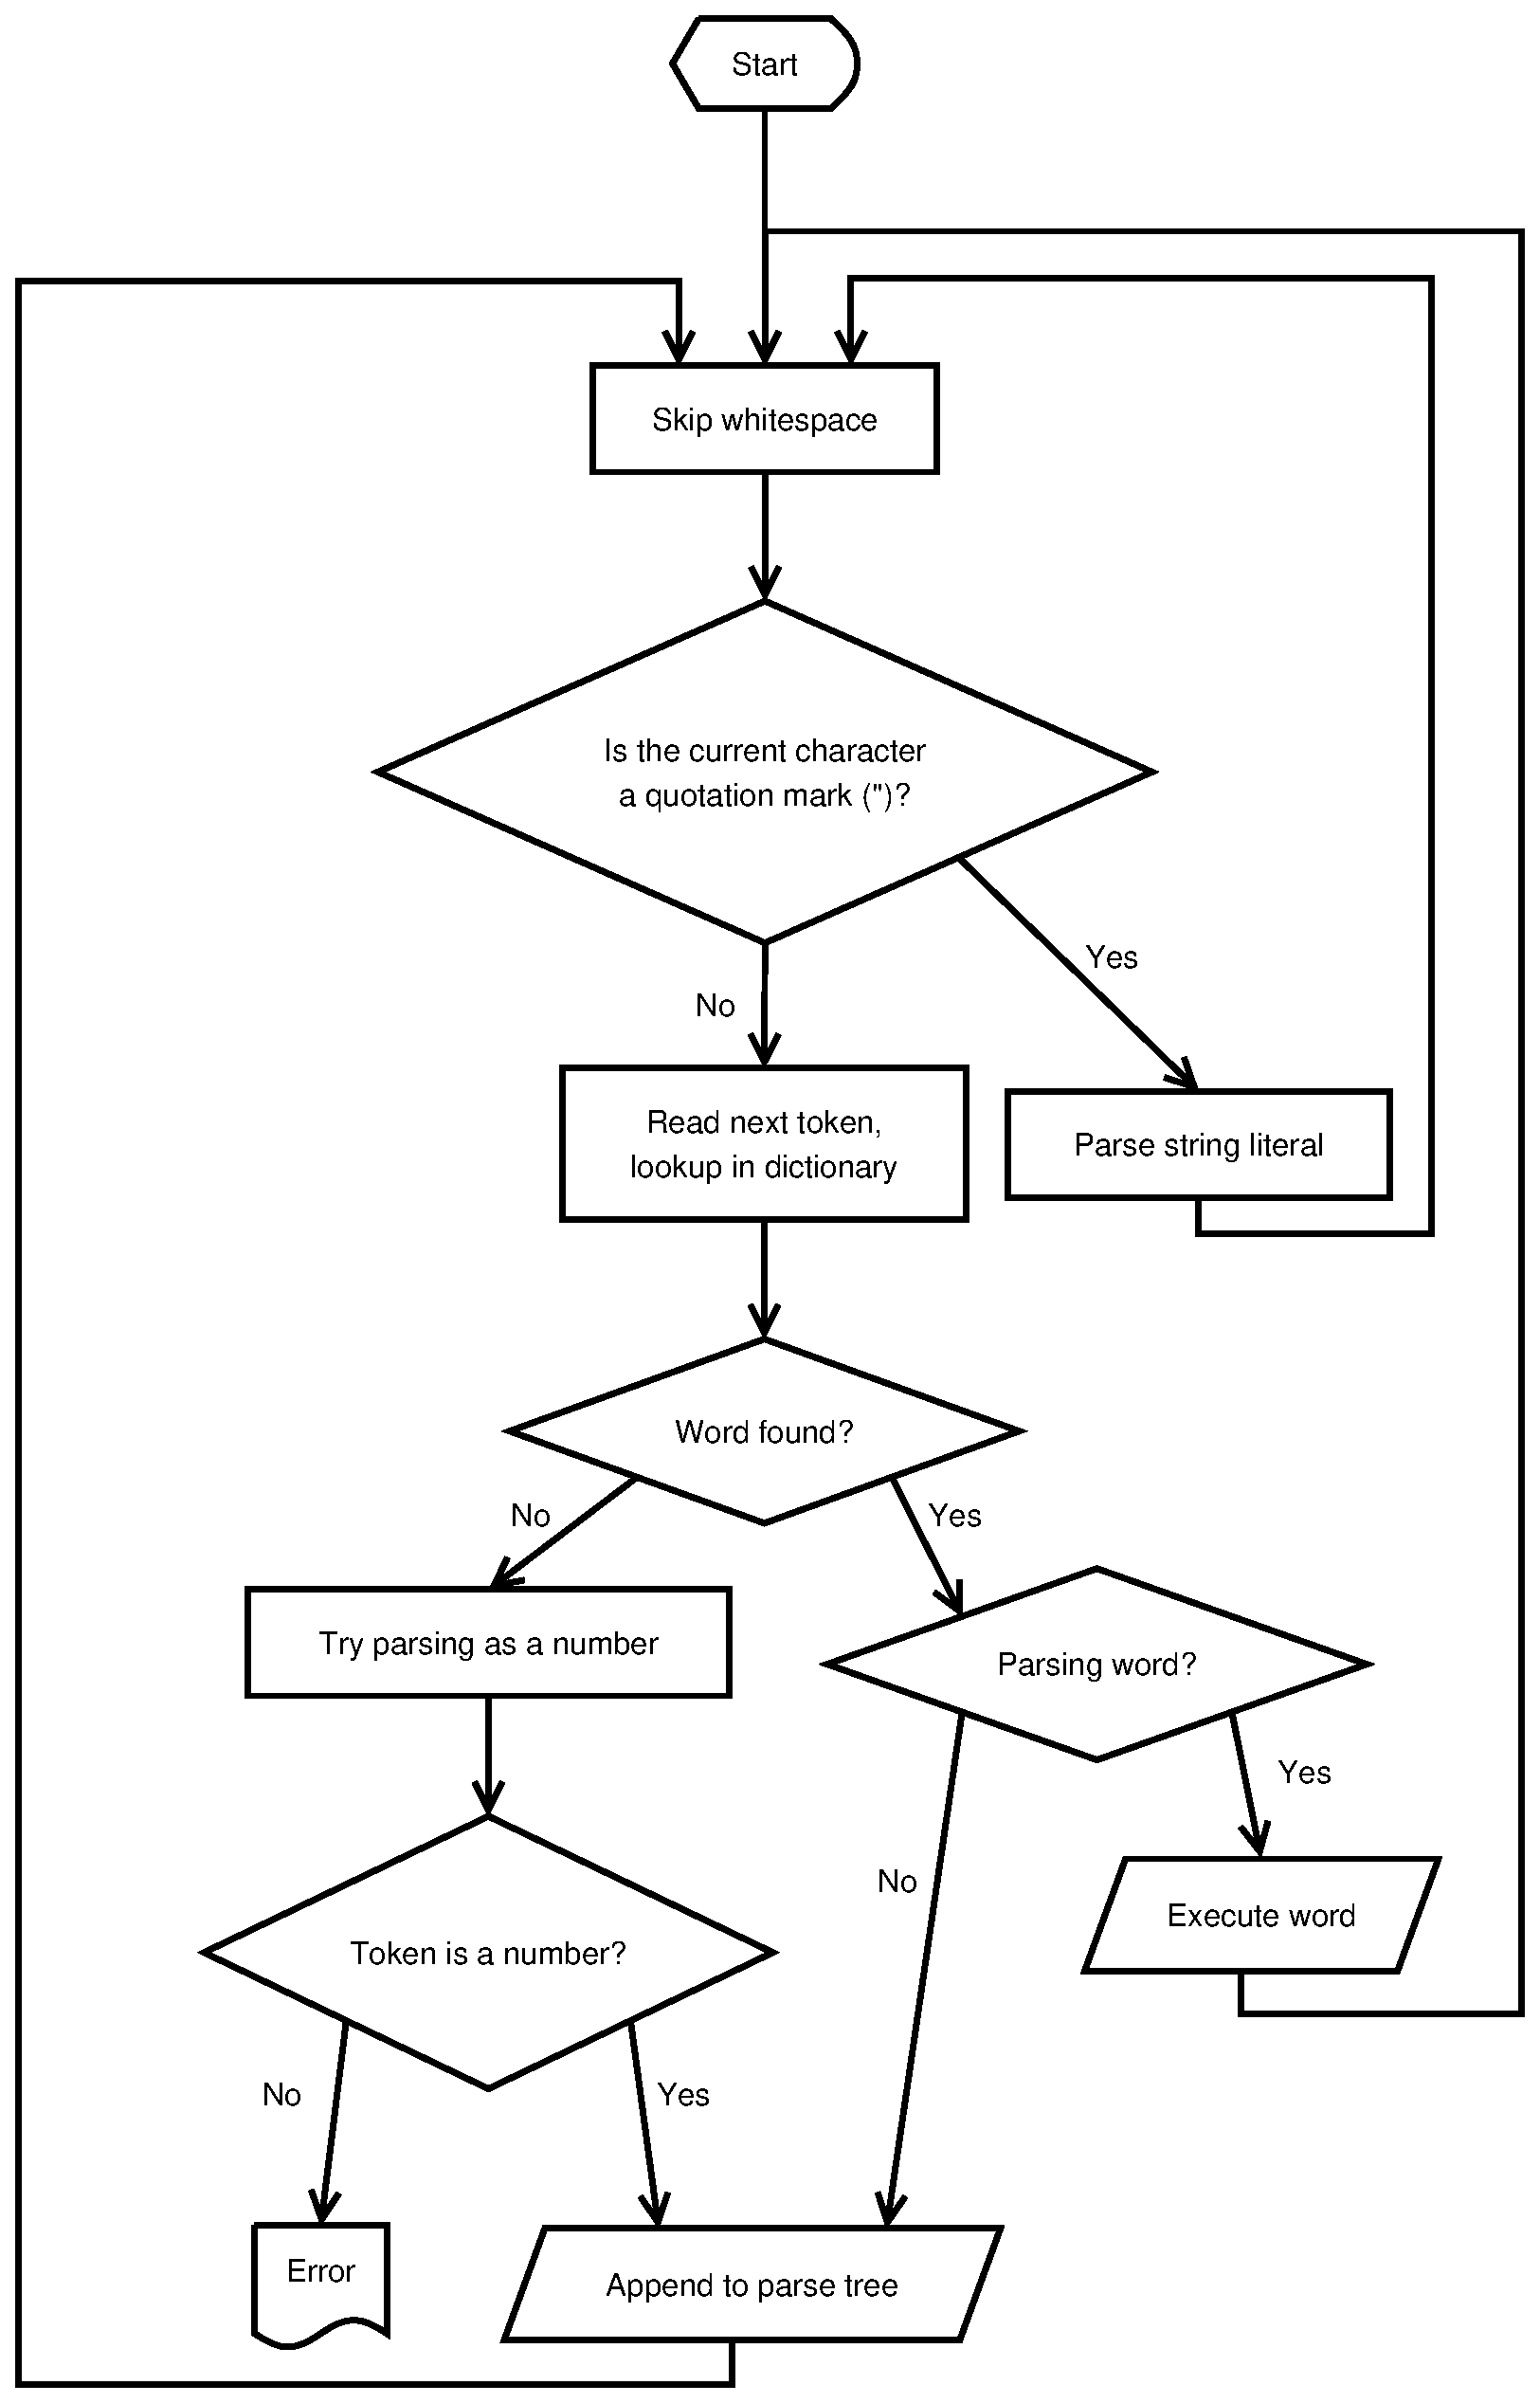
\epsfig{file=parser.eps}}
\end{center}
\end{figure}

At the most abstract level,
Factor syntax consists of whitespace-separated tokens. The parser tokenizes the input on whitespace boundaries, where whitespace is defined as a sequence or one or more space, tab, newline or carriage-return characters.  The parser is case-sensitive, so
the following three expressions tokenize differently:
\begin{verbatim}
2X+
2 X +
2 x +
\end{verbatim}
As the parser reads tokens it makes a distinction between numbers, ordinary words, and
parsing words. Tokens are appended to the parse tree, the top level of which is a list
returned by the original parser invocation. Nested levels of the parse tree are created
by parsing words.

Here is the parser algorithm in more detail -- some of the concepts therein will be defined shortly:

\begin{itemize}
\item If the current character is a double-quote (\texttt{"}), the \texttt{"} parsing word is executed, causing a string to be read.
\item Otherwise, the next token is taken from the input. The parser searches for a word named by the token in the currently used set of vocabularies. If the word is found, one of the following two actions is taken:
\begin{itemize}
\item If the word is an ordinary word, it is appended to the parse tree.
\item If the word is a parsing word, it is executed.
\end{itemize}
Otherwise if the token does not represent a known word, the parser attempts to parse it as a number. If the token is a number, the number object is added to the parse tree. Otherwise, an error is raised and parsing halts.
\end{itemize}

\glossary{name=string mode,
description={a parser mode where token strings are added to the parse tree; the parser will not look up tokens in the dictionary. Activated by switching on the \texttt{string-mode} variable}}

There is one exception to the above process; the parser might be placed in \emph{string mode}, in which case it simply reads tokens and appends them to the parse tree as strings. String mode is activated and deactivated by certain parsing words wishing to read input in an unstructured but tokenized manner -- see \ref{string-mode}.

\glossary{name=parsing word,
description={a word that is run at parse time. Parsing words can be defined by suffixing the compound definition with \texttt{parsing}. Parsing words have the \texttt{\dq{}parsing\dq{}} word property set to true, and respond with true to the \texttt{parsing?}~word}}

Parsing words play a key role in parsing; while ordinary words and numbers are simply
added to the parse tree, parsing words execute in the context of the parser, and can
do their own parsing and create nested data structures in the parse tree. Parsing words
are also able to define new words.

While parsing words supporting arbitrary syntax can be defined, the default set is found
in the \texttt{syntax} vocabulary and provides the basis for all further syntactic
interaction with Factor.

\subsection{\label{vocabsearch}Vocabulary search}

\newcommand{\wordglos}{\glossary{
name=word,
description={an object holding a code definition and set of properties. Words are organized into vocabularies, and are uniquely identified by name within a vocabulary.}}}
\wordglos
\newcommand{\vocabglos}{\glossary{
name=vocabulary,
description={a collection of words, uniquely identified by name. The hashtable of vocabularies is stored in the \texttt{vocabularies} global variable, and the \texttt{USE:}~and \texttt{USING:}~parsing words add vocabularies to the parser's search path}}}
\vocabglos

A \emph{word} associates a code definition with its name. Words are organized into \emph{vocabularies}. Vocabularies are organized into vocabularies. Words are discussed in depth in \ref{words}.

When the parser reads a token, it attempts to look up a word named by that token. The
lookup is performed in the parser's current vocabulary set. By default, this set includes
two vocabularies:
\begin{verbatim}
syntax
scratchpad
\end{verbatim}
The \texttt{syntax} vocabulary consists of a set of parsing words for reading Factor data
and defining new words. The \texttt{scratchpad} vocabulary is the default vocabulary for new
word definitions.
\wordtable{
\parsingword{USE:}{USE: \emph{vocabulary}}{syntax}
}
\newcommand{\useglos}{\glossary{
name=search path,
description={the list of vocabularies that the parser looks up tokens in. You can add to this list with the \texttt{USE:} and \texttt{USING:} parsing words}}}
\useglos

The \texttt{USE:} parsing word adds a new vocabulary at the front of the search path. Subsequent word lookups by the parser will search this vocabulary first.
\begin{alltt}
USE: lists
\end{alltt}
\wordtable{
\parsingword{USING:}{USING: \emph{vocabularies} ;}{syntax}
}
Consecutive \texttt{USE:} declarations can be merged into a single \texttt{USING:} declaration.
\begin{alltt}
USING: lists strings vectors ;
\end{alltt}

Due to the way the parser works, words cannot be referenced before they are defined; that is, source files must order definitions in a strictly bottom-up fashion. For a way around this, see \ref{deferred}.

\subsection{Numbers}

\newcommand{\numberglos}{\glossary{
name=number,
description={an instance of the \texttt{number} class}}}
\numberglos

If a vocabulary lookup of a token fails, the parser attempts to parse it as a number.

\subsubsection{Integers}

\newcommand{\integerglos}{\glossary{
name=integer,
description={an instance of the \texttt{integer} class, which is a disjoint union of the \texttt{fixnum} and \texttt{bignum} classes}}}
\numberglos

\newcommand{\fixnumglos}{\glossary{
name=fixnum,
description={an instance of the \texttt{fixnum} class, representing a fixed precision integer. On 32-bit systems, an element of the interval $(-2^{-29},2^{29}]$, and on 64-bit systems, the interval $(-2^{-61},2^{61}]$}}}
\fixnumglos

\newcommand{\bignumglos}{\glossary{
name=bignum,
description={an instance of the \texttt{bignum} class, representing an arbitrary-precision integer whose value is bounded by available object memory}}}
\bignumglos

The printed representation of an integer consists of a sequence of digits, optionally prefixed by a sign.
\begin{alltt}
123456
-10
2432902008176640000
\end{alltt}
Integers are entered in base 10 unless prefixed with a base change parsing word.
\wordtable{
\parsingword{BIN:}{BIN: \emph{integer}}{syntax}\\
\parsingword{OCT:}{OCT: \emph{integer}}{syntax}\\
\parsingword{HEX:}{HEX: \emph{integer}}{syntax}
}
\begin{alltt}
\textbf{ok} BIN: 1110 BIN: 1 + .
\textbf{15}
\textbf{ok} HEX: deadbeef 2 * .
\textbf{7471857118}
\end{alltt}

\subsubsection{Ratios}

\newcommand{\ratioglos}{\glossary{
name=ratio,
description={an instance of the \texttt{ratio} class, representing an exact ratio of two integers}}}
\ratioglos

The printed representation of a ratio is a pair of integers separated by a slash (\texttt{/}).
No intermediate whitespace is permitted. Either integer may be signed, however the ratio will be normalized into a form where the denominator is positive and the greatest common divisor
of the two terms is 1.
\begin{alltt}
75/33
1/10
-5/-6
\end{alltt}

\subsubsection{Floats}

\newcommand{\floatglos}{\glossary{
name=float,
description={an instance of the \texttt{float} class, representing an IEEE 754 double-precision floating point number}}}
\floatglos

Floating point numbers contain an optional decimal part, an optional exponent, with
an optional sign prefix on either the significand or exponent.
\begin{alltt}
10.5
-3.1456
7e13
1e-5
\end{alltt}

\subsubsection{Complex numbers}

\newcommand{\complexglos}{\glossary{
name=complex,
description={an instance of the \texttt{complex} class, representing a complex number with real and imaginary components, where both components are real numbers}}}
\complexglos
\wordtable{
\parsingword{hash-curly}{\#\{ \emph{real} \emph{imaginary} \}\#}{syntax}
}
A complex number
is given by two components, a ``real'' part and ''imaginary'' part. The components
must either be integers, ratios or floats.
\begin{verbatim}
#{ 1/2 1/3 }#   ! the complex number 1/2+1/3i
#{ 0 1 }#       ! the imaginary unit
\end{verbatim}

\subsection{Literals}

Many different types of objects can be constructed at parse time via literal syntax. Numbers are a special case since support for reading them is built-in to the parser. All other literals are constructed via parsing words.

If a quotation contains a literal object, the same literal object instance is used each time the quotation executes; that is, literals are ``live''.

\subsubsection{\label{boolean}Booleans}

\newcommand{\boolglos}{
\glossary{
name=boolean,
description={an instance of the \texttt{boolean} class, either \texttt{f} or \texttt{t}. See generalized boolean}}
\glossary{
name=generalized boolean,
description={an object used as a truth value. The \texttt{f} object is false and anything else is true. See boolean}}
\glossary{
name=t,
description={the canonical truth value. The \texttt{t} class, whose sole instance is the \texttt{t} object. Note that the \texttt{t} class is not equal to the \texttt{t} object}}
\glossary{
name=f,
description={the canonical false value; anything else is true. The \texttt{f} class, whose sole instance is the \texttt{f} object. Note that the \texttt{f} class is not equal to the \texttt{f} object}}
}
\boolglos
Any Factor object may be used as a truth value in a conditional expression. The \texttt{f} object is false and anything else is true. The \texttt{f} object is also used to represent the empty list, as well as the concept of a missing value. The canonical truth value is the \texttt{t} object.
\wordtable{
\parsingword{f}{f}{syntax}\\
\parsingword{t}{t}{syntax}
}
Adds the \texttt{f} and \texttt{t} objects to the parse tree.

Note that the \texttt{f} parsing word and class is not the same as the \texttt{f} object. The former can be obtained by writing \texttt{\bs~f} inside a quotation, or \texttt{POSTPONE: f} inside a list that will not be evaluated.
\begin{alltt}
\textbf{ok} f \bs f = .
\textbf{f}
\end{alltt}
An analogous distinction holds for the \texttt{t} class and object.

\subsubsection{\label{syntax:char}Characters}

\newcommand{\charglos}{\glossary{
name=character,
description={an integer whose value denotes a Unicode code point. Character values are limited to the range from $0$ to $2^16-1$ inclusive, however in a later release this can be upgraded to the full 21-bit Unicode space without requiring any changes to user code}}}
\charglos
Factor has no distinct character type, however Unicode character value integers can be
read by specifying a literal character, or an escaped representation thereof.
\wordtable{
\parsingword{CHAR:}{CHAR: \emph{token}}{syntax}
}
Adds the Unicode code point of the character represented by \emph{token} to the parse tree.

\newcommand{\escapeglos}{\glossary{
name=escape,
description={a sequence allowing a non-literal character to be inserted in a string. For a list of escapes, see \ref{escape}}}}
\escapeglos
If the token is a single-character string other than whitespace or backslash, the character is taken to be this token. If the token begins with a backslash, it denotes one of the following escape codes.
\begin{table}[Special character escape codes]
\label{escape}
\begin{tabular}{l|l}
Escape code&Character\\
\hline
\texttt{\bs{}\bs}&Backslash (\texttt{\bs})\\
\texttt{\bs{}s}&Space\\
\texttt{\bs{}t}&Tab\\
\texttt{\bs{}n}&Newline\\
\texttt{\bs{}t}&Carriage return\\
\texttt{\bs{}0}&Null byte (ASCII 0)\\
\texttt{\bs{}e}&Escape (ASCII 27)\\
\texttt{\bs{}"}&Double quote (\texttt{"})\\
\end{tabular}
\end{table}
Examples:
\begin{alltt}
\textbf{ok} CHAR: a .
\textbf{97}
\textbf{ok} CHAR: \bs{}0 .
\textbf{0}
\textbf{ok} CHAR: \bs{}n .
\textbf{10}
\end{alltt}
A Unicode character can be specified by its code number by writing \texttt{\bs{}u} followed by a four-digit hexadecimal. That is, the following two expressions are equivalent:
\begin{alltt}
CHAR: \bs{}u0078
78
\end{alltt}
While not useful for single characters, this syntax is also permitted inside strings.

\subsubsection{\label{string-literals}Strings}

\newcommand{\stringglos}{\glossary{
name=string,
description={an instance of the \texttt{string} class, representing an immutable sequence of characters}}}
\stringglos
\wordtable{
\parsingword{"}{"\emph{string}"}{syntax}
}
Reads from the input string until the next occurrence of
\texttt{"}, and appends the resulting string to the parse tree. String literals cannot span multiple lines.
Strings containing
the \texttt{"} character and various other special characters can be read by
inserting escape sequences as described in \ref{syntax:char}.
\begin{alltt}
\textbf{ok} "Hello world" print
\textbf{Hello world}
\end{alltt}

\subsubsection{\label{listsyntax}Lists}
\newcommand{\listglos}{\glossary{
name=list,
description={an instance of the \texttt{list} class, storing a sequence of elements as a chain of zero or more conses, where the car of each cons is an element, and the cdr is either \texttt{f} or another list}}
\glossary{name=proper list, description=see list}
}
\listglos
\wordtable{
\parsingword{openbracket}{[}{syntax}\\
\parsingword{closebracket}{]}{syntax}
}
Parses a list, whose elements are read between \texttt{[} and \texttt{]} and can include other lists.
\begin{verbatim}
[
    "404" "responder" set
    [ drop no-such-responder ] "get" set
]
\end{verbatim}
\newcommand{\consglos}{\glossary{
name=cons,
description={an instance of the \texttt{cons} class, storing an ordered pair of objects referred to as the car and the cdr}}}
\consglos
\wordtable{
\parsingword{conssyntax}{[[ \emph{car} \emph{cdr} ]]}{syntax}
}
Parses two components making up a cons cell. Note that the lists parsed with \texttt{[} and \texttt{]} are just a special case of \texttt{[[} and \texttt{]]}. The following two lines are equivalent.
\begin{alltt}
[ 1 2 3 ]
[[ 1 [[ 2 [[ 3 f ]] ]] ]]
\end{alltt}
The empty list is denoted by \texttt{f}, along with boolean falsity, and the concept of a missing value. The expression \texttt{[ ]} parses to the same object as \texttt{f}.

\subsubsection{Words}

While words parse as themselves, a word occurring inside a quotation is executed when the quotation is called. Sometimes it is desirable to have a word be pushed on the data stack during the execution of a quotation, usually for reflective access to the word's slots.
\wordtable{
\parsingword{bs}{\bs~\emph{word}}{syntax}
}
Reads the next word from the input string and appends some \emph{code} to the parse tree that pushes the word on the stack when the code is called. The following two lines are equivalent:
\begin{verbatim}
\ length
[ length ] car
\end{verbatim}
\wordtable{
\parsingword{POSTPONE:}{POSTPONE: \emph{word}}{syntax}
}
Reads the next word from the input string and appends the word to the parse tree, even if it is a parsing word. For an word \texttt{foo}, \texttt{POSTPONE: foo} and \texttt{foo} are equivalent; however, if \texttt{foo} is a parsing word, the latter will execute it at parse time, while the former will execute it at runtime. Usually used inside parsing words that wish to delegate some action to a further parsing word.
\begin{alltt}
\textbf{ok} : parsing1
    "Parsing 1" print 2 swons ; parsing
\textbf{ok} : parsing2
    "Parsing 2" print POSTPONE: parsing1 ; parsing
\textbf{ok} [ 1 parsing1 3 ] .
\textbf{Parsing 1}
\textbf{[ 1 2 3 ]}
\textbf{ok} [ 0 parsing2 2 4 ] .
\textbf{Parsing 2}
\textbf{Parsing 1}
\textbf{[ 0 2 4 ]}
\end{alltt}

\subsubsection{Mutable literals}

\newcommand{\mutableglos}{\glossary{name=mutable object,
description=an object whose slot values can be changed}
\glossary{name=immutable object,
description=an object whose slot values cannot be changed}}
\mutableglos

Using mutable object literals in word definitions requires care, since if those objects
are mutated, the actual word definition will be changed, which is in most cases not what you would expect. Strings and lists are immutable; string buffers, vectors, hashtables and tuples are mutable.

\subsubsection{\label{sbuf-literals}String buffers}

\newcommand{\sbufglos}{\glossary{
name=string buffer,
description={an instance of the \texttt{sbuf} class, representing a mutable and growable sequence of characters}}
\glossary{name=sbuf, description=see string buffer}}
\sbufglos
\wordtable{
\parsingword{SBUF}{SBUF" \emph{text}"}{syntax}
}
Reads from the input string until the next occurrence of
\texttt{"}, converts the string to a string buffer, and appends it to the parse tree.
As with strings, the escape codes described in \ref{syntax:char} are permitted.
\begin{alltt}
\textbf{ok} SBUF" Hello world" sbuf>string print
\textbf{Hello world}
\end{alltt}

\subsubsection{\label{vector-literals}Vectors}
\newcommand{\vectorglos}{\glossary{
name=vector,
description={an instance of the \texttt{vector} class, storing a mutable and growable sequence of elements in a contiguous range of memory}}}
\vectorglos
\wordtable{
\parsingword{opencurly}{\{}{syntax}\\
\parsingword{closecurly}{\}}{syntax}
}
Parses a vector, whose elements are read between \texttt{\{} and \texttt{\}}.
\begin{verbatim}
{ 3 "blind" "mice" }
\end{verbatim}

\subsubsection{Hashtables}
\newcommand{\hashglos}{\glossary{
name=hashtable,
description={an instance of the \texttt{hashtable} class, providing a mutable mapping of keys to values}}}
\hashglos
\wordtable{
\parsingword{openccurly}{\{\{}{syntax}\\
\parsingword{closeccurly}{\}\}}{syntax}
}
Parses a hashtable. Elements between \texttt{\{\{} and \texttt{\}\}} must be cons cells, where the car is the key and the cdr is a value.
\begin{verbatim}
{{
    [[ "red" [ 255 0 0 ] ]]
    [[ "green" [ 0 255 0 ] ]]
    [[ "blue" [ 0 0 255 ] ]]
}}
\end{verbatim}

\subsubsection{Tuples}
\newcommand{\tupleglos}{\glossary{
name=tuple,
description={an instance of a user-defined class whose metaclass is the \texttt{tuple} metaclass, storing a fixed set of elements in named slots, with optional delegation method dispatch semantics}}}
\tupleglos
\wordtable{
\parsingword{<<}{<<}{syntax}\\
\parsingword{>>}{>>}{syntax}
}
Parses a tuple. The tuple's class must follow \texttt{<<}. The element after that is always the tuple's delegate. Further elements until \texttt{>>} are specified according to the tuple's slot definition, and an error is raised if an incorrect number of elements is given.
\begin{verbatim}
<< color f 255 0 0 >>
\end{verbatim}

\subsection{\label{comments}Comments}

\wordtable{
\parsingword{!}{!~\emph{remainder of line}}{syntax}
}
The remainder of the input line is ignored if an exclamation mark (\texttt{!}) is read.
\begin{alltt}
! Note that the sequence union does not include lists,
! or user defined tuples that respond to the sequence
! protocol.
\end{alltt}
\wordtable{
\parsingword{hash!}{\#!~\emph{remainder of line}}{syntax}
}
\newcommand{\doccommentglos}{\glossary{
name=documentation comment,
description={a comment describing the usage of a word. Delimited by the \texttt{\#"!} parsing word, they appear at the start of a word definition and are stored in the \texttt{""documentation""} word property}}}
\doccommentglos
Comments that begin with \texttt{\#!} are called \emph{documentation comments}.
A documentation comment has no effect on the generated parse tree, but if it is the first thing inside a word definition, the comment text is appended to the string stored in the word's \texttt{"documentation"} property. Word properties are described in \ref{word-props}.
\wordtable{
\parsingword{(}{( \emph{stack effect} )}{syntax}
}
\glossary{
name=stack effect,
description={A string of the form \texttt{( \emph{inputs} -- \emph{outputs} )}, where the inputs and outputs are a whitespace-separated list of names or types. The top of the stack is the right-most token on both sides.}}
\newcommand{\stackcommentglos}{\glossary{
name=stack effect comment,
description={a comment describing the inputs and outputs of a word. Delimited by \texttt{(} and \texttt{}), they appear at the start of a word definition and are stored in the \texttt{""stack-effect""} word property}}}
\stackcommentglos
Comments delimited by \texttt{(} and \texttt{)} are called \emph{stack effect comments}. By convention they are placed at the beginning of a word definition to document the word's inputs and outputs:
\begin{verbatim}
: push ( element sequence -- )
    #! Push a value on the end of a sequence.
    dup length swap set-nth ;
\end{verbatim}
A stack effect comment has no effect on the generated parse tree, but if it is the first thing inside a word definition, the word's \texttt{"stack-effect"} property is set to the comment text. Word properties are described in \ref{word-props}.

\section{Data and control flow}

\subsection{Shuffle words}

\newcommand{\dsglos}{\glossary{
name=stack,
description=see data stack}
\glossary{
name=data stack,
description={the primary means of passing values between words}}}
\dsglos
Shuffle words are placed between words taking action to rearrange items on the stack
as the next word in the quotation would expect them. Their behavior can be understood entirely in terms of their stack effects.
\wordtable{
\ordinaryword{drop}{drop ( x -- )}{kernel}\\
\ordinaryword{2drop}{drop ( x y -- )}{kernel}\\
\ordinaryword{3drop}{drop ( x y z -- )}{kernel}\\
\ordinaryword{nip}{nip ( x y -- y )}{kernel}\\
\ordinaryword{2nip}{2nip ( x y -- y )}{kernel}\\
\ordinaryword{dup}{dup ( x -- x x )}{kernel}\\
\ordinaryword{2dup}{2dup ( x y -- x y x y )}{kernel}\\
\ordinaryword{3dup}{3dup ( x y z -- x y z x y z )}{kernel}\\
\ordinaryword{dupd}{dupd ( x y -- x x y )}{kernel}\\
\ordinaryword{over}{over ( x y -- x y x )}{kernel}\\
\ordinaryword{pick}{pick ( x y z -- x y z x )}{kernel}\\
\ordinaryword{tuck}{tuck ( x y -- y x y )}{kernel}\\
\ordinaryword{swap}{swap ( x y -- y x )}{kernel}\\
\ordinaryword{2swap}{2swap ( x y z t -- z t x y )}{kernel}\\
\ordinaryword{swapd}{swapd ( x y z -- y x z )}{kernel}\\
\ordinaryword{rot}{rot ( x y z -- y z x )}{kernel}\\
\ordinaryword{-rot}{-rot ( x y z -- z x y )}{kernel}
}
Try to avoid the complex shuffle words such as \texttt{rot} and \texttt{2dup} as much as possible, for they make data flow harder to understand. If you find yourself using too many shuffle words, or you're writing
a stack effect comment in the middle of a compound definition to keep track of stack contents, it is
a good sign that the word should probably be factored into two or
more smaller words.

\subsection{\label{quotations}Quotations}

\newcommand{\csglos}{\glossary{
name=return stack,
description=see call stack}
\glossary{
name=call stack,
description={holds quotations waiting to be called. When a quotation is called with \texttt{call}, or when a compound word is executed, the previous call frame is pushed on the call stack, and the new quotation becomes the current call frame}}}
\csglos
\newcommand{\cfglos}{\glossary{
name=call frame,
description=the currently executing quotation}}
\cfglos
\glossary{
name=interpreter,
description=executes quotations by iterating them and recursing into nested definitions. see compiler}

\begin{figure}
\begin{center}
\caption{Interpreter algorithm}
\scalebox{0.45}{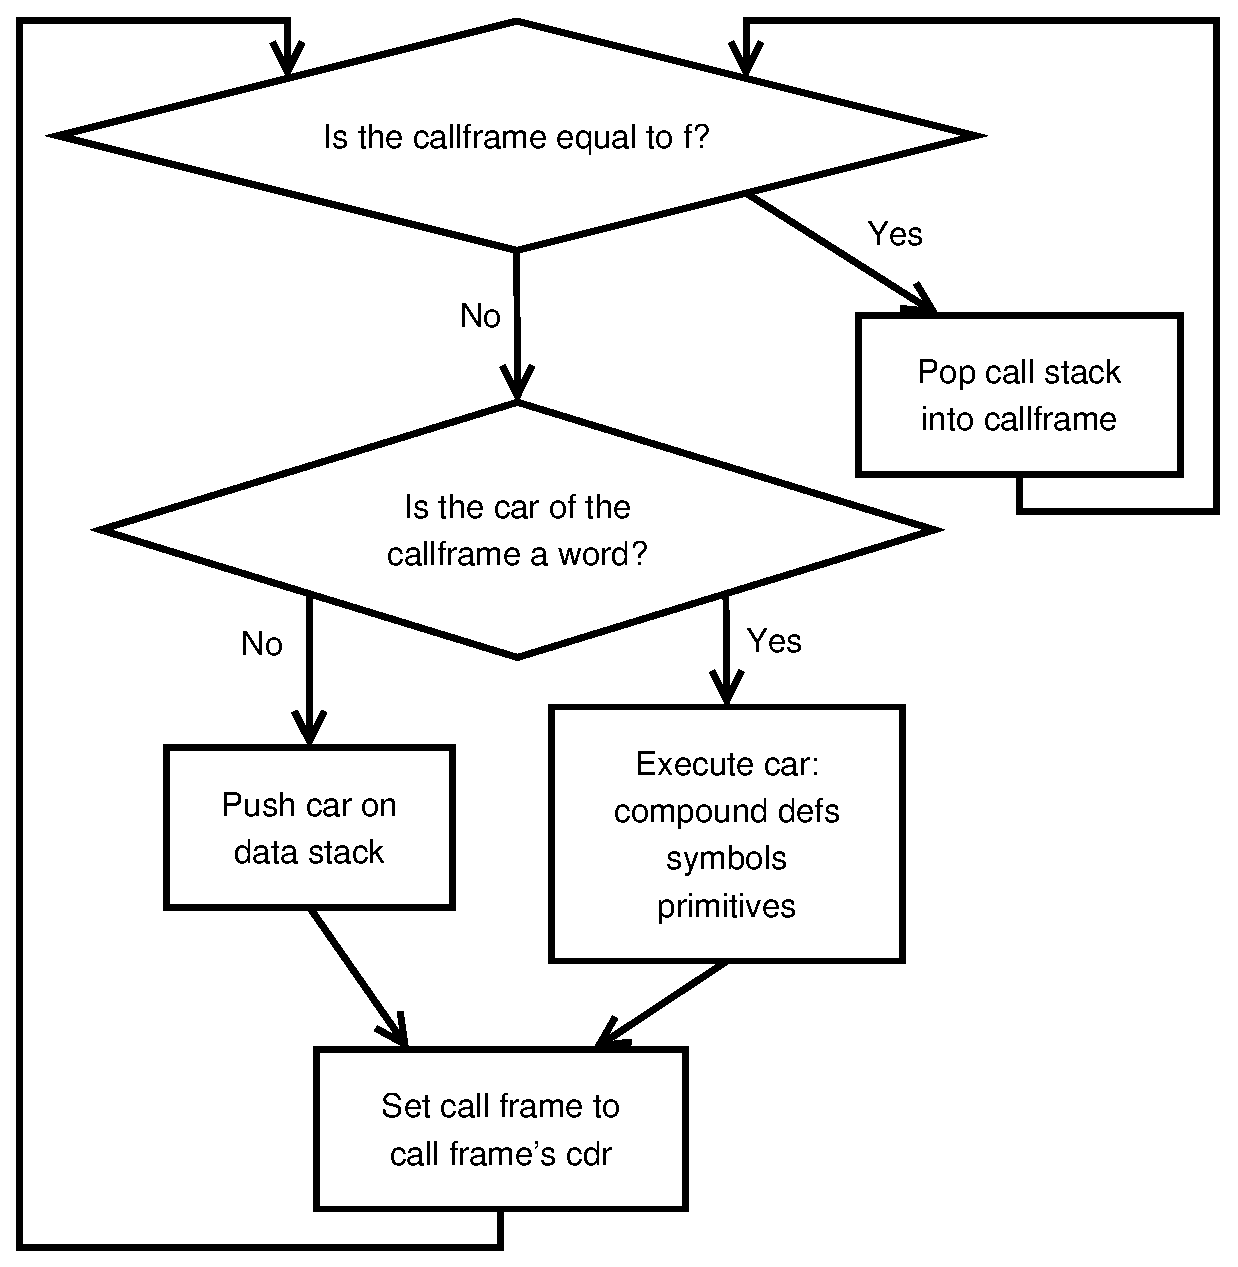
\epsfig{file=interpreter.eps}}
\end{center}
\end{figure}

The Factor interpreter executes quotations. Quotations are lists, and since lists can contain any Factor object, they can contain words. It is words that give quotations their operational behavior, as you can see in the following description of the interpreter algorithm.

\begin{itemize}
\item If the call frame is \texttt{f}, the call stack is popped and becomes the new call frame.
\item If the car of the call frame is a word, the word is executed:
\begin{itemize}
\item If the word is a symbol, it is pushed on the data stack. See \ref{symbols}.
\item If the word is a compound definition, the current call frame is pushed on the call stack, and the new call frame becomes the word definition. See \ref{colondefs}.
\item If the word is compiled or primitive, the interpreter jumps to a machine code definition. See \ref{primitives}.
\item If the word is undefined, an error is raised. See \ref{deferred}.
\end{itemize}
\item Otherwise, the car of the call frame is pushed on the data stack.
\item The call frame is set to the cdr, and the loop continues.
\end{itemize}

The interpreter can be invoked reflectively with the following pair of words.
\wordtable{
\ordinaryword{call}{call ( quot -- )}{kernel}
}
Push the current call frame on the call stack, and set the call stack to the given quotation. Conceptually: calls the quotation, as if its definition was substituted at the location of the \texttt{call}.
\begin{alltt}
\textbf{ok} [ 2 2 + 3 * ] call .
\textbf{12}
\end{alltt}
\wordtable{
\ordinaryword{execute}{execute ( word -- )}{kernel}
}
Execute a word definition, taking action based on the word definition, as above.
\begin{alltt}
\textbf{ok} : hello "Hello world" print ;
\textbf{ok} : twice dup execute execute ;
\textbf{ok} \bs hello twice
\textbf{Hello world}
\textbf{Hello world}
\end{alltt}

\subsubsection{Tail call optimization}

\newcommand{\tailglos}{\glossary{
name=tail call,
description=the last call in a quotation}
\glossary{
name=tail call optimization,
description=the elimination of call stack pushes when making a tail call}}

When a call is made to a quotation from the last word in the call frame, there is no
purpose in pushing the empty call frame on the call stack. Therefore the last call in a quotation does not grow the call stack, and tail recursion executes in bounded space.

\subsubsection{Call stack manipulation}

Because of the way the interpreter is described in \ref{quotations}, the top of the call stack is not accessed during the execution of a quotation; it is only popped when the interpreter reaches the end of the quotation. In effect, the call stack can be used as a temporary storage area, as long as pushes and pops are balanced out within a single quotation.
\wordtable{
\ordinaryword{>r}{>r ( x -- r:x )}{kernel}
}
Moves the top of the data stack to the call stack.
\wordtable{
\ordinaryword{r>}{r> ( x -- r:x )}{kernel}
}
Moves the top of the call stack to the data stack.

The top of the data stack is ``hidden'' between \texttt{>r} and \texttt{r>}.
\begin{alltt}
\textbf{ok} 1 2 3 >r .s r>
\textbf{2
1}
\end{alltt}
It is very important to balance usages of \texttt{>r} and \texttt{r>} within a single quotation or word definition.
\begin{verbatim}
: the-good >r 2 + r> * ; ! Okay
: the-bad  >r 2 + ;      ! Runtime error
: the-ugly r> ;          ! Runtime error
\end{verbatim}
Basically, the rule is you must leave the call stack in the same state as you found it, so that when the current quotation finishes executing, the interpreter can return to the caller.

One exception is that when \texttt{ifte} occurs as the last word in a definition, values may be pushed on the call stack before the condition value is computed, as long as both branches of the \texttt{ifte} pop the values off the call stack before returning.
\begin{verbatim}
: foo ( m ? n -- m+n/n )
    >r [ r> + ] [ drop r> ] ifte ; ! Okay
\end{verbatim}

\subsubsection{Quotation variants}

There are three words that combine shuffle words with \texttt{call}. They are useful in the implementation of higher-order words taking quotations as inputs.
\wordtable{
\ordinaryword{slip}{slip ( quot x -- x | quot: -- )}{kernel}
}
Call a quotation, while hiding the top of the stack. The implementation is as you would expect.
\begin{verbatim}
: slip ( quot x -- x | quot: -- )
    >r call r> ; inline
\end{verbatim}
\wordtable{
\ordinaryword{keep}{keep ( x quot -- x | quot:~x -- )}{kernel}
}
Call a quotation with a value on the stack, restoring the value when the quotation returns.
\begin{verbatim}
: keep ( x quot -- x | quot: x -- )
    over >r call r> ; inline
\end{verbatim}
\wordtable{
\ordinaryword{2keep}{2keep ( x y q -- x y | q:~x y -- )}{kernel}
}
Call a quotation with a pair of values on the stack, restoring the values when the quotation returns.
\begin{verbatim}
: 2keep ( x y quot -- x y | quot: x y -- )
    over >r pick >r call r> r> ; inline
\end{verbatim}

\subsection{Conditionals}

The simplest style of a conditional form is the \texttt{ifte} word.
\wordtable{
\ordinaryword{ifte}{ifte ( cond true false -- )}{kernel}
}
The \texttt{cond} is a generalized boolean. If it is \texttt{f}, the \texttt{false} quotation is called, and if \texttt{cond} is any other value, the \texttt{true} quotation is called. The condition flag is removed from the stack before either quotation executes.

Note that in general, both branches should have the same stack effect. Not only is this good style that makes the word easier to understand, but also unbalanced conditionals cannot be compiled.
\wordtable{
\ordinaryword{when}{when ( cond true -- | true:~-- )}{kernel}\\
\ordinaryword{unless}{unless ( cond false -- | false:~-- )}{kernel}
}
This pair are minor variations on \texttt{ifte} where only one branch is specified. The other is implicitly \texttt{[ ]}. They are implemented in the trivial way:
\begin{verbatim}
: when [ ] ifte ; inline
: unless [ ] swap ifte ; inline
\end{verbatim}
The \texttt{ifte} word removes the condition flag from the stack before calling either quotation. Sometimes this is not desirable, if the condition flag is serving a dual purpose as a value to be consumed by the \texttt{true} quotation. The \texttt{ifte*} word exists for this purpose.
\wordtable{
\ordinaryword{ifte*}{ifte*~( cond true false -- )}{kernel}\\
\texttt{true:~cond --}\\
\texttt{false:~--}
}
If the condition is true, it is retained on the stack before the \texttt{true} quotation is called. Otherwise, the condition is removed from the stack and the \texttt{false} quotation is called. The following two lines are equivalent:
\begin{verbatim}
X [ Y ] [ Z ] ifte*
X dup [ Y ] [ drop Z ] ifte
\end{verbatim}
\wordtable{
\ordinaryword{when*}{when*~( cond true -- | true:~cond -- )}{kernel}\\
\ordinaryword{unless*}{unless*~( cond false -- | false:~-- )}{kernel}
}
These are variations of \texttt{ifte*} where one of the quotations is \texttt{[ ]}.

There is one final conditional form that is used to implement the ``default value'' idiom.
\wordtable{
\ordinaryword{?ifte}{?ifte ( default cond true false -- )}{kernel}\\
\texttt{true:~cond --}\\
\texttt{false:~default --}
}
If the condition is \texttt{f}, the \texttt{false} quotation is called with the \texttt{default} value on the stack. Otherwise, the \texttt{true} quotation is called with the condition on the stack. The following two lines are equivalent:
\begin{verbatim}
X [ Y ] [ Z ] ?ifte
X dup [ nip Y ] [ drop Z ] ifte
\end{verbatim}

\subsubsection{Boolean logic}

The \texttt{?}~word chooses between two values, rather than two quotations.
\wordtable{
\ordinaryword{?}{?~( cond true false -- true/false )}{kernel}
}
It is implemented in the obvious way.
\begin{verbatim}
: ? ( cond t f -- t/f )
    rot [ drop ] [ nip ] ifte ; inline
\end{verbatim}
Several words use \texttt{?}~to implement typical boolean algebraic operations.
\wordtable{
\ordinaryword{>boolean}{>boolean ( obj -- t/f )}{kernel}
}
Convert a generalized boolean into a boolean. That is, \texttt{f} retains its value, whereas anything else becomes \texttt{t}.
\wordtable{
\ordinaryword{not}{not ( ?~-- ?~)}{kernel}
}
Given \texttt{f}, outputs \texttt{t}, and on any other input, outputs \texttt{f}.
\wordtable{
\ordinaryword{and}{and ( ?~?~-- ?~)}{kernel}
}
Outputs \texttt{t} if both of the inputs are true.
\wordtable{
\ordinaryword{or}{or ( ?~?~-- ?~)}{kernel}
}
Outputs \texttt{t} if at least one of the inputs is true.
\wordtable{
\ordinaryword{xor}{xor ( ?~?~-- ?~)}{kernel}
}
Outputs \texttt{t} if exactly one of the inputs is true.
\wordtable{
\ordinaryword{implies}{implies ( b1~b2~-- ?~)}{kernel}
}
Outputs \texttt{t} if \texttt{b1} is false or both inputs are true.

An alternative set of logical operations operate on individual bits of integers bitwise, rather than generalized boolean truth values. They are documented in \ref{bitwise}.

\subsection{Continuations}

\newcommand{\contglos}{
\glossary{name=continuation,
description=an object representing the future of the computation}}
\contglos
At any point in the execution of a Factor program, the \emph{current continuation} represents the future of the computation. This object can be captured with the \texttt{callcc0} and \texttt{callcc1} words.
\wordtable{
\ordinaryword{callcc0}{callcc0 ( quot -- )}{kernel}\\
\texttt{quot:~cont --}\\
\texttt{cont:~--}\\
\ordinaryword{callcc1}{callcc1 ( quot -- )}{kernel}\\
\texttt{quot:~cont --}\\
\texttt{cont:~obj --}
}
Calling one of these words calls the given quotation with the continuation on the stack. The continuation is itself a quotation, and calling it \emph{continues execution} at the point after the call to \texttt{callcc0} and \texttt{callcc1}. Essentially, a continuation is a snapshot of the four stacks that can be restored at a later time.

The difference between \texttt{callcc0} and \texttt{callcc1} lies in the continuation object. When \texttt{callcc1} is used, calling the continuation takes one value from the top of the data stack, and places it back on the \emph{restored} data stack. This allows idioms such as exception handling, co-routines and generators to be implemented via continuations.

\subsubsection{\label{exceptions}Handling exceptional situations}
\glossary{name=exception,
description=an object representing an exceptional situation that has been detected}

Support for handling exceptional situations such as bad user input, implementation bugs, and input/output errors is provided by a pair of words, \texttt{throw} and \texttt{catch}.
\wordtable{
\ordinaryword{throw}{throw ( exception -- )}{errors}
}
Raises an exception. Execution does not continue at the point after the \texttt{throw} call. Rather, the innermost catch block is invoked, and execution continues at that point. Passing \texttt{f} as an exception will cause \texttt{throw} to do nothing.
\wordtable{
\ordinaryword{catch}{catch ( try handler -- )}{errors}\\
\texttt{handler:~exception/f -- }
}
An exception handler is established, and the \texttt{try} quotation is called.

If the \texttt{try} quotation throws an error and no nested \texttt{catch} is established, the following sequence of events takes place:
\begin{itemize}
\item the stacks are restored to their state prior to the \texttt{catch} call,
\item the exception is pushed on the data stack,
\item the \texttt{handler} quotation is called.
\end{itemize}
If the \texttt{try} quotation completes successfully, the stacks are \emph{not} restored. The \texttt{f} object is pushed, and the \texttt{handler} quotation is called.

A common idiom is that the \texttt{catch} block cleans up from the error in some fashion, then passes it on to the next-innermost catch block. The following word is used for this purpose.
\wordtable{
\ordinaryword{rethrow}{throw ( exception -- )}{errors}
}
Raises an exception, without saving the current stacks for post-mortem inspection. This is done so that inspecting the error stacks sheds light on the original cause of the exception, rather than the point where it was rethrown.

Here is a simple example of a word definition that attempts to convert a string representing a hexadecimal number into an integer, and instead of halting execution when the string is not valid, it simply outputs \texttt{f}.
\begin{verbatim}
: catch-hex> ( str -- n/f )
    [ hex> ] [ [ drop f ] when ] catch ;
\end{verbatim}
Exception handling is implemented using a \emph{catch stack}. The \texttt{catch} word pushes the current continuation on the catch stack, and \texttt{throw} calls the continuation at the top of the catch stack with the raised exception.
\glossary{name=catch stack,
description={a stack of exception handler continuations, pushed and popped by \texttt{catch}}}

\subsubsection{Multitasking}

Factor implements co-operative multitasking, where the thread of control switches between tasks at explicit calls to \texttt{yield}, as well as when blocking I/O is performed. Multitasking is implemented via continuations.
\wordtable{
\ordinaryword{in-thread}{in-thread ( quot -- )}{threads}
}
Calls \texttt{quot} in a co-operative thread. The new thread begins executing immediately, and the current thread resumes when the quotation yields, either from blocking
I/O or an explicit call to \texttt{yield}. This is implemented by adding the current continuation to the run queue, then calling \texttt{quot}, and finally executing \texttt{stop} after \texttt{quot} returns.
\wordtable{
\ordinaryword{yield}{yield ( -- )}{threads}
}
Add the current continuation to the end of the run queue, and call the continuation at the front of the run queue.
\wordtable{
\ordinaryword{stop}{stop ( -- )}{threads}
}
Call the continuation at the front of run queue, without saving the current continuation. In effect, this stops the current thread.

\subsubsection{Interpreter state}

The current state of the interpreter is determined by the contents of the four stacks. A set of words for getting and setting stack contents are the primitive building blocks for continuations, and in turn abstractions such as exception handling and multitasking.
\wordtable{
\ordinaryword{datastack}{datastack ( -- vector )}{kernel}\\
\ordinaryword{set-datastack}{set-datastack ( vector -- )}{kernel}
}
Save and restore the data stack contents. As an example, here is a word that executes a quotation and restores the data stack to its previous state;
\begin{verbatim}
: keep-datastack
    ( quot -- ) datastack slip set-datastack drop ;
\end{verbatim}
Note that the \texttt{drop} call is made to remove the original quotation from the stack.
\wordtable{
\ordinaryword{callstack}{callstack ( -- vector )}{kernel}\\
\ordinaryword{set-callstack}{set-callstack ( vector -- )}{kernel}
}
Save and restore the call stack contents. The call stack does not include the currently executing quotation that made the call to \texttt{callstack}, since the current quotation is held in the call frame -- \ref{quotations} has details. Similarly, calling \texttt{set-callstack} will continue executing the current quotation until it returns, at which point control transfers to the quotation at the top of the new call stack.
\wordtable{
\ordinaryword{namestack}{namestack ( -- list )}{namespaces}\\
\ordinaryword{set-namestack}{set-namestack ( list -- )}{namespaces}
}
Save and restore the name stack, used for dynamic variable bindings. See \ref{namespaces}.
\wordtable{
\ordinaryword{catchstack}{catchstack ( -- list )}{errors}\\
\ordinaryword{set-catchstack}{set-catchstack ( list -- )}{errors}
}
Save and restore the catch stack, used for exception handling. See \ref{exceptions}.

\section{\label{words}Words}

\wordglos
\vocabglos
\glossary{name=defining word,
description=a word that adds definitions to the dictionary}
\glossary{name=dictionary,
description=the collection of vocabularies making up the code in the Factor image}
Words are the fundamental unit of code in Factor, analogous to functions or procedures in other languages. Words are also objects, and this concept forms the basis for Factor's meta-programming facilities. Words hold two distinct pieces of information:
\begin{itemize}
\item A definition, specifying the behavior of the word when executed,
\item A set of word properties, including the name of the word, its vocabulary, any documentation strings, and other meta-data.
\end{itemize}
\wordtable{
\ordinaryword{word?}{word?~( object -- ?~)}{words}
}
Tests if the \texttt{object} is a word.
\wordtable{
\classword{word}{words}
}
The class of words.

\subsection{Vocabularies}
\wordtable{
\symbolword{vocabularies}{words}
}
Words are organized into named vocabularies, stored in the global \texttt{vocabularies} variable.
\wordtable{
\parsingword{IN:}{IN:~\emph{vocabulary}}{syntax}
}
Sets the current vocabulary for new word definitions, and adds the vocabulary to the search path (\ref{vocabsearch}).

Parsing words add definitions to the current vocabulary. When a source file is being parsed, the current vocabulary is initially set to \texttt{scratchpad}.

\subsubsection{Searching for words}

Words whose names are known at parse time -- that is, most words making up your program -- can be referenced by stating their name. However, the parser itself, and sometimes code you write, will need to look up words dynamically.
\wordtable{
\ordinaryword{search}{search ( name vocabs -- word )}{words}
}
The \texttt{vocabs} parameter is a list of vocabulary names. If a word with the given name is found, it is pushed on the stack, otherwise, \texttt{f} is pushed.

\subsubsection{Creating words}

\wordtable{
\ordinaryword{create}{create ( name vocabulary -- word )}{words}
}
Creates a new word \texttt{name} in \texttt{vocabulary}. If the vocabulary already contains a word with this name, the existing word is returned.
\wordtable{
\ordinaryword{create-in}{create-in ( name -- word )}{words}
}
Creates a new word \texttt{name} in the current vocabulary. Should only be called from parsing words (\ref{parsing-words}), and in fact is defined as:
\begin{verbatim}
: create-in ( name -- word ) "in" get create ;
\end{verbatim}

\subsection{Word definition}

There are two ways to create a word definition:
\begin{itemize}
\item Using parsing words at parse time,
\item Using defining words at run-time. This is a more dynamic feature that can be used to implement code generation and such, and in fact parse-time defining words are implemented in terms of run-time defining words.
\end{itemize}

\subsubsection{\label{colondefs}Compound definitions}

\newcommand{\colonglos}{\glossary{
name=compound definition,
description=a word defined to execute a quotation consisting of existing words}
\glossary{
name=colon definition,
description=see compound definition}}
\colonglos
A compound definition associates a word name with a quotation that is called when the word is executed.
\wordtable{
\parsingword{:}{:~\emph{name} \emph{definition} ;}{syntax}
}
A word \texttt{name} is created in the current vocabulary, and is associated with \texttt{definition}.
\begin{verbatim}
: ask-name ( -- name )
    "What is your name? " write read-line ;
: greet ( name -- )
    "Greetings, " write print ;
: friend ( -- )
    ask-name greet ;
\end{verbatim}
By convention, the word name should be followed by a stack effect comment, and for more complex definitions, a documentation comment; see \ref{comments}.
\wordtable{
\ordinaryword{define-compound}{define-compound ( word quotation -- )}{words}
}
Defines \texttt{word} to call the \texttt{quotation} when executed.
\wordtable{
\ordinaryword{compound?}{compound?~( object -- ?~)}{words}
}
Tests if the \texttt{object} is a compound word definition.
\wordtable{
\classword{compound}{words}
}
The class that all compound words are an instance of.

\subsubsection{\label{symbols}Symbols}

\newcommand{\symbolglos}{\glossary{
name=symbol,
description={a word defined to push itself on the stack when executed, created by the \texttt{SYMBOL:}~parsing word}}}
\symbolglos
\wordtable{
\parsingword{SYMBOL:}{SYMBOL:~\emph{name}}{syntax}
}
A word \texttt{name} is created in the current vocabulary that pushes itself on the stack when executed. Symbols are used to identify variables (\ref{namespaces}) as well as for storing crufties in their properties (\ref{word-props}).
\wordtable{
\ordinaryword{define-symbol}{define-symbol ( word -- )}{words}
}
Defines \texttt{word} to push itself on the data stack when executed.
\wordtable{
\ordinaryword{symbol?}{symbol?~( object -- ?~)}{words}
}
Tests if the \texttt{object} is a symbol.
\wordtable{
\classword{symbol}{words}
}
The class that all symbols are an instance of.

\subsubsection{\label{primitives}Primitives}
\newcommand{\primglos}{\glossary{
name=primitive,
description=a word implemented as native code in the Factor runtime}}
\symbolglos

Executing a primitive invokes native code in the Factor runtime. Primitives cannot be defined through Factor code. Compiled definitions behave similarly to primitives in that the interpreter jumps to native code upon encountering them.
\wordtable{
\ordinaryword{primitive?}{primitive?~( object -- ?~)}{words}
}
Tests if the \texttt{object} is a primitive.
\wordtable{
\classword{primitive}{words}
}
The class that all primitives are an instance of.

\subsubsection{\label{deferred}Deferred words and mutual recursion}

\glossary{
name=deferred word,
description={a word without a definition, created by the \texttt{DEFER:}~parsing word}}
Due to the way the parser works, words cannot be referenced before they are defined; that is, source files must order definitions in a strictly bottom-up fashion. Mutually-recursive pairs of words can be implemented by \emph{deferring} one of the words in the pair so that the second word in the pair can parse, then by replacing the deferred definition with a real one.
A demonstration of the idiom:
\begin{verbatim}
DEFER: foe
: fie ... foe ... ;
: foe ... fie ... ;
\end{verbatim}
\wordtable{
\parsingword{DEFER:}{DEFER:~\emph{name}}{syntax}
}
Create a word \texttt{name} in the current vocabulary that simply raises an error when executed. Usually, the word will be replaced with a real definition later.
\wordtable{
\ordinaryword{undefined?}{undefined?~( object -- ?~)}{words}
}
Tests if the \texttt{object} is an undefined (deferred) word.
\wordtable{
\classword{undefined}{words}
}
The class that all undefined words are an instance of.

\subsubsection{Undefining words}

\wordtable{
\parsingword{FORGET:}{FORGET:~\emph{name}}{syntax}
}
Removes the word \texttt{name} from its vocabulary. Existing definitions that reference the word will continue to work, but newly-parsed occurrences of the word will not locate the forgotten definition. No exception is thrown if no such word exists.
\wordtable{
\ordinaryword{forget}{forget ( word -- )}{words}
}
Removes the word from its vocabulary. The parsing word \texttt{FORGET:} is implemented using this word.

\subsection{\label{word-props}Word properties}

\glossary{name=word property,
description={a name/value pair stored in a word's properties}}
\glossary{name=word properties,
description={a hashtable associated with each word storing various sundry properties}}

Each word has an associated hashtable of properties. Conventionally, the property names are strings, but nothing requires that this be so.

A common idiom in the Factor library is to use symbols for their properties. 

\wordtable{
\ordinaryword{word-prop}{word-prop ( word name -- value )}{words}\\
\ordinaryword{set-word-prop}{set-word-prop ( value word name -- )}{words}
}
Retrieve and store word properties. Note that the stack effect is designed so that it is most convenient when \texttt{name} is a literal that is pushed on the stack right before executing these words. This is usually the case.

\wordtable{
\ordinaryword{word-name}{word-prop ( word -- name )}{words}\\
\ordinaryword{word-vocabulary}{word-vocabulary ( word -- vocabulary )}{words}
}
Retreive the name of a word, and the name of the vocabulary it is stored in. The definitions are trivial:
\begin{verbatim}
: word-name "name" word-prop ;
: word-vocabulary "vocabulary" word-prop ;
\end{verbatim}

\wordtable{
\ordinaryword{word-sort}{word-sort ( list -- list )}{words}
}
Sort a list of words by name.

\wordtable{
\ordinaryword{word-props}{word-props ( word -- hashtable )}{words}\\
\ordinaryword{set-word-props}{set-word-props ( hashtable word -- )}{words}
}
Retreive and store the entire set of word properties.

\subsection{Low-level details}

The actual behavior of a word when executed is determined by the values of two slots:
\begin{itemize}
\item The primitive number
\item The primitive parameter
\end{itemize}
The primitive number is an index into an array of native functions in the Factor runtime.
Some frequently-occurring primitive numbers:
\begin{description}
\item[0] deferred word,
\item[1] compound definition -- executes the quotation stored in the parameter slot,
\item[2] symbol -- pushes the value of the parameter slot,
\item[3 onwards] the actual set of primitives, of which there are around 170.
\end{description}
The words outlined in this section should not be used in ordinary code.
\wordtable{
\ordinaryword{word-primitive}{word-primitive ( word -- n )}{words}\\
\ordinaryword{set-word-primitive}{set-word-primitive ( word -- n )}{words}
}
Retrieves and stores a word's primitive number.

\wordtable{
\ordinaryword{word-def}{word-def ( word -- object )}{words}\\
\ordinaryword{set-word-def}{set-word-def ( object word -- )}{words}
}
Retrieves and stores a word's primitive parameter. This parameter is only used if the primitive number is 1 (compound definitions) or 2 (symbols). Note that to define a compound definition or symbol, you must use \texttt{define-compound} or \texttt{define-symbol}, as these words do not update the cross-referencing of word dependencies.

\wordtable{
\ordinaryword{word-xt}{word-xt ( word -- n )}{words}\\
\ordinaryword{set-word-xt}{set-word-xt ( n word -- )}{words}
}
Retrieves and stores a word's \emph{execution token}.

This is an even lower-level facility for working with the address containing native code to be invoked when the word is executed. The compiler sets the execution token to a location in memory containing generated code.

\wordtable{
\ordinaryword{update-xt}{update-xt ( word -- )}{words}
}
Updates a word's execution token according to its primitive number. When called with a compiled word, has the effect of decompiling the word. The execution token is automatically updated after a call to \texttt{set-word-primitive}.

\wordtable{
\ordinaryword{recrossref}{recrossref ( word -- )}{words}
}
Updates the cross-referencing database, which you will probably need to do if you mess around with any of the words in this section -- assuming Factor does not crash first, that is.

\chapter{The library}

\section{Objects}

\glossary{name=object,
description=a datum that can be identified}
\mutableglos

Everything in Factor is an object, where an object is a collection of slots. Each object has a unique identity, and references to objects are passed by value on the stack. It is possible to have two references to the same object, and if the object is mutated through one reference, the changes will be visible through the other reference. Not all objects are mutable; the documentation for each class details if its instances are mutable or not.

\subsection{\label{equality}Identity and equality}

\glossary{name=equal,
description={two objects are equal if they have the same class and if their slots are equal, or alternatively, if both are numbers that denote the same value}}
There are two distinct notions of ``sameness'' when it comes to objects. You can test if two references point to the same object, or you can test if two objects are equal in some sense, usually by having the same type and equal slot values.
\wordtable{
\ordinaryword{eq?}{eq?~( object object -- ?~)}{kernel}
}
Output \texttt{t} if two references point to the same object, and \texttt{f} otherwise.
\wordtable{
\genericword{=}{= ( object object -- ?~)}{kernel}
}
Output \texttt{t} if two objects are equal, and \texttt{f} otherwise. The precise meaning of equality depends on the object's class, however usually two objects are equal if their slot values are equal. If two objects are equal, they have the same printed representation, although the converse is not always true. In particular:
\begin{itemize}
\item If no more specific method is defined, \texttt{=} calls \texttt{eq?}.
\item Two numbers are equal if they have the same numerical value.
\item Two sequences are equal if they are both instances of the same class, and if they have the same length, and elements.
\item Two hashtables are equal if they hold the same set of key/value pairs.
\item Two tuples are equal if they are of the same class and their slots are equal.
\item Two words are equal if they are the same object.
\end{itemize}
\wordtable{
\genericword{clone}{clone ( object -- object )}{kernel}
}
Make a fresh object that is equal to the given object. This is not guaranteed to actually copy the object; it does nothing with immutable objects, and does not copy words either. However, sequences and tuples can be cloned to obtain a new shallow copy of the original.

\subsection{Generic words and methods}

\glossary{name=generic word,
description={a word defined using the \texttt{GENERIC:}~parsing word. The behavior of generic words depends on the class of the object at the top of the stack. A generic word is composed of methods, where each method is specialized on a class}}
\glossary{name=method,
description={gives a generic word behavior when the top of the stack is an instance of a specific class}}
Sometimes  you want a word's behavior to depend on the class of the object at the top of the stack, however implementing the word as a set of nested conditional tests is undesirable since it leads to unnecessary coupling -- adding support for a new class requires modifying the original definition of the word.

A generic word is a word whose behavior depends on the class of the
object at the top of the stack, however this behavior is defined in a
decentralized manner.

\wordtable{
\parsingword{GENERIC:}{GENERIC: \emph{word}}{syntax}
}
Defines a new generic word. Initially, it contains no methods, and thus will raise an error when called.

\wordtable{
\parsingword{M:}{M: \emph{class} \emph{word} \emph{definition} ;}{syntax}
}
Defines a method, that is, a behavior for the generic \texttt{word} specialized on instances of \texttt{class}. Each method definition
can potentially occur in a different source file.

\subsubsection{\label{method-order}Method ordering}

If two classes have a non-empty intersection, there is no guarantee that one is a subclass of the other. This means there is no canonical linear ordering of classes. The methods of a generic word are linearly ordered, though, and you can inspect this order using the \texttt{order} word.

Suppose you have the following definitions:
\begin{verbatim}
GENERIC: foo
M: integer foo 1 + ;
M: number foo 1 - ;
M: object foo dup 2list ;
\end{verbatim}
Since the \texttt{integer} class is strictly smaller than the \texttt{number} class, which in turn is strictly smaller than the \texttt{object} class, the ordering of methods is not surprising in this case:
\begin{alltt}
\textbf{ok} \bs foo order .
\textbf{[ object number integer ]}
\end{alltt}
However, suppose we had the following set of definitions:
\begin{verbatim}
GENERIC: describe
M: general-t describe drop "a true value" print ;
M: general-list describe drop "a list" print ;
M: object describe drop "an object" print ;
\end{verbatim}
Neither \texttt{general-t} nor \texttt{general-list} contains the other, and their intersection is the non-empty \texttt{cons} class. So the generic word system will place \texttt{object} first in the method order, however either \texttt{general-t} or \texttt{general-list} may come next, and it is pretty much a random choice that depends on hashing:
\begin{alltt}
\textbf{ok} \bs bar order .
\textbf{[ object general-list general-t ]}
\end{alltt}

Therefore, the outcome of calling \texttt{bar} with a cons cell is undefined.

\subsection{Classes}
\glossary{name=class,
description=a set of objects defined in a formal manner. Methods specialize generic words on classes}
\glossary{name=metaclass,
description={a set of classes sharing common traits. Examples include \texttt{builtin}, \texttt{union}, and \texttt{tuple}}}

\wordtable{
\classword{object}{generic}
}
Every object is a member of the \texttt{object} class. If you provide a method specializing
on the \texttt{object} class for some generic word, the method will be
invoked when no more specific method exists. For example:
\begin{verbatim}
GENERIC: describe
M: number describe
    "The number " write . ;
M: object describe
    "I don't know anything about " write . ;
\end{verbatim}
Each class has a membership predicate named
after the class with a \texttt{?}~suffix, with the following exceptions:
\begin{description}
\item[object] there is no need for a predicate word, since
every object is an instance of this class.
\item[f] the only instance of this class is the singleton
\texttt{f} signifying falsity, missing value, and empty list, and the predicate testing for this is the built-in library word \texttt{not}.
\item[t] the only instance of this class is the canonical truth value
\texttt{t}. You can write \texttt{t =} to test for this object, however usually
any object distinct from \texttt{f} is taken as a truth value, and \texttt{t} is not tested for directly.
\end{description}

\subsubsection{Built-in classes}
\glossary{name=type,
description={an object invariant that describes its shape. An object's type is constant for the lifetime of the object, and there is only a fixed number of types built-in to the run-time. See class}}
\glossary{name=built-in class,
description=see type}
Every object is an instance of to exactly one type, and the type is constant for the lifetime of the object. There is only a fixed number of types built-in to the run-time, and corresponding to each type is a \emph{built-in class}:
\begin{verbatim}
alien
array
bignum
byte-array
complex
cons
dll
f
fixnum
float
ratio
sbuf
string
t
tuple
vector
word
\end{verbatim}
\wordtable{
\ordinaryword{type}{type ( object -- n )}{kernel}
}
Outputs the type number of a given object. Most often, the \texttt{class} word is more useful.
\wordtable{
\ordinaryword{class}{class ( object -- class )}{kernel}
}
Outputs the canonical class of a given object. While an object may be an instance of more than one class, the canonical class is either the built-in class, or if the object is a tuple, the tuple class. Examples:
\begin{alltt}
\textbf{ok} 1.0 class .
\textbf{float}
\textbf{ok} TUPLE: point x y z ;
\textbf{ok} << point f 1 2 3 >> class .
\textbf{point}
\end{alltt}

\subsubsection{Unions}
\glossary{name=union,
description={a class whose set of instances is the union of the set of instances of a list of member classes}}
An object is an instance of a union class if it is an instance of one of its members. Union classes are used to associate the same method with several different classes, as well as to conveniently define predicates.
\wordtable{
\parsingword{UNION:}{UNION: \emph{name} \emph{members} ;}{syntax}
}
Defines a union class. For example, the Factor library defines some unions over numeric types:
\begin{verbatim}
UNION: integer fixnum bignum ;
UNION: rational integer ratio ;
UNION: real rational float ;
UNION: number real complex ;
\end{verbatim}
Now, the absolute value function can be defined in an efficient manner
for real numbers, and in a more general fashion for complex numbers:
\begin{verbatim}
GENERIC: abs ( z -- |z| )
M: real abs dup 0 < [ neg ] when ;
M: complex abs >rect mag2 ;
\end{verbatim}

\subsubsection{Complements}
\glossary{name=complement,
description={a class whose set of instances is the set of objects that are not instances of a specific class}}

An object is an instance of a complement if it is not an instance of the complement's parameter.
\wordtable{
\parsingword{COMPLEMENT:}{COMPLEMENT: \emph{name} \emph{parameter}}{syntax}
}
Defines a complement class. For example, the class of all values denoting ``true'' is defined as follows:
\begin{verbatim}
COMPLEMENT: general-t f
\end{verbatim}

\subsubsection{Predicates}
\glossary{name=predicate,
description={a word with stack effect \texttt{( object -- ?~)}, or more alternatively, a class whose instances are the instances of a superclass that satisfy an arbitrary predicate}}
An object is an instance of a predicate classes if it is an instance of the predicate's parent class, and if it satisfies the predicate definition.

Each predicate must be
defined as a subclass of some other class. This ensures that predicates inheriting from disjoint classes do not need to be
exhaustively tested during method dispatch.
\wordtable{
\parsingword{PREDICATE:}{PREDICATE: \emph{parent} \emph{name} \emph{predicate} ;}{syntax}
}
Defines a predicate class deriving from \texttt{parent} whose instances are the instances of \texttt{superclass} that satisfy the \texttt{predicate} quotation. The predicate quotation must have stack effect \texttt{( object -- ?~)}.

For example, the \texttt{strings} vocabulary contains subclasses of \texttt{integer}
classifying various ASCII characters:
\begin{verbatim}
PREDICATE: integer blank     " \t\n\r" str-contains? ;
PREDICATE: integer letter    CHAR: a CHAR: z between? ;
PREDICATE: integer LETTER    CHAR: A CHAR: Z between? ;
PREDICATE: integer digit     CHAR: 0 CHAR: 9 between? ;
PREDICATE: integer printable CHAR: \s CHAR: ~ between? ;
\end{verbatim}

\subsubsection{Operations on classes}
\wordtable{
\ordinaryword{class-and}{class-and ( class class -- class )}{kernel}\\
\ordinaryword{class-or}{class-or ( class class -- class )}{kernel}
}
Intersection and union of classes. Note that the returned class might not be the exact desired class; for example, \texttt{object} is output if no suitable class definition could be found at all.
\wordtable{
\ordinaryword{class<}{class< ( class class -- class )}{kernel}
}
Classes are partially ordered. This ordering determines the method ordering of a generic word (\ref{method-order}).

\subsection{Tuples}
\tupleglos

Tuples are user-defined classes composed of named slots. All tuples have the same type, however distinct classes of tuples are defined.
\wordtable{
\parsingword{TUPLE:}{TUPLE: \emph{name} \emph{slots} ;}{syntax}
}
Defines a new tuple class with membership predicate \texttt{name?}~and constructor \texttt{<name>}.

The constructor takes slots in left-to-right order from the stack. After construction, slots are read and written using various automatically-defined words with names of the
form \texttt{\emph{class}-\emph{slot}} and \texttt{set-\emph{class}-\emph{slot}}.

Here is an example:
\begin{verbatim}
TUPLE: point x y z ;
\end{verbatim}
This defines a new class named \texttt{point}, along with the
following set of words:
\begin{verbatim}
<point> point?
point-x set-point-x
point-y set-point-y
point-z set-point-z
\end{verbatim}
The word \texttt{<point>} takes the slot values from the stack and
produces a new \texttt{point}:
\begin{alltt}
\textbf{ok} 1 2 3 <point> .
\textbf{<< point 1 2 3 >>}
\end{alltt}

\subsubsection{Constructors}

Constructors are named after the tuple class surrounded in angle
brackets (\texttt{<}~and~\texttt{>}). A default constructor is provided
that reads slot values from the stack, however a custom constructor can
be defined using the \texttt{C:} parsing word.
\wordtable{
\parsingword{C:}{C: \emph{class} \emph{definition} ;}{syntax}
}
Define a \texttt{<class>} word that creates a tuple instance of the \texttt{class}, then applies the \texttt{definition} to this new tuple. The \texttt{definition} quotation must have stack effect \texttt{( tuple -- tuple )}.

\subsubsection{Delegation}

\glossary{name=delegate,
description={a fa\,cade object's delegate receives unhandled methods that are called on the fa\,cade}}
\glossary{name={fa\,cade},
description=an object with a delegate}

Each tuple can have an optional delegate tuple. Generic words called on
the tuple that do not have a method for the tuple's class will be passed on
to the delegate. Note that delegation to objects that are not tuples is not fully supported at this stage and might not work as you might expect.
\wordtable{
\ordinaryword{delegate}{delegate ( object -- object )}{syntax}
}
Returns an object's delegate, or \texttt{f} if no delegate is set. Note that in this case,  undefined methods will be passed to \texttt{f}; rather an error is raised immediately.
\wordtable{
\ordinaryword{set-delegate}{set-delegate ( object tuple -- )}{syntax}
}
Sets a tuple's delegate.

Factor uses delegation is used instead of inheritance, but it is not a direct
substitute; in particular, the semantics differ in that a delegated
method call receives the delegate on the stack, not the original object.

\section{Sequences}

\glossary{name=sequence,
description=an object storing a linearly-ordered set of elements}
A sequence is a linearly-ordered collection of objects. A set of built-in sequence types  is provided by the library.

\begin{tabular}[t]{l|c|c|c|c|c|l}
\multicolumn{4}{l|}{}&\multicolumn{2}{c|}{Adding elements}&\multicolumn{1}{l}{}\\
\hline
Class&Mutable&Growable&Lookup&at start&at end&Primary purpose\\
\hline
\texttt{array}&$\surd$&&$O(1)$&&&Low-level and unsafe (\ref{unsafe})\\
\texttt{list}&&&$O(n)$&$O(1)$&$O(n)$&Functional manipulation\\
\texttt{vector}&$\surd$&$\surd$&$O(1)$&$O(n)$&$O(1)$&Imperitive aggregation\\
\texttt{sbuf}&$\surd$&$\surd$&$O(1)$&$O(n)$&$O(1)$&Character accumilation\\
\texttt{string}&&&$O(1)$&&&Immutable text strings
\end{tabular}

Additionally, user-defined classes can implement the sequence protocol and gain the ability to reuse many of the words in this section.

\subsection{Sequence protocol}

The following set of generic words is the core of the sequence protocol. The mutating words are not supported by all sequences; in particular, lists and strings are immutable.

\glossary{name=resizable sequence,
description={a sequence implementing the \texttt{set-length} generic word. For example, vectors and string buffers}}
\glossary{name=mutable sequence,
description={a sequence implementing the \texttt{set-nth} generic word. For example, vectors and string buffers}}
The sequence protocol consists of a set of generic words. Any object that is an instance of a class implementing these generic words can be thought of as a sequence, and given to the words in the following sections.

\wordtable{
\genericword{length}{length ( seq -- n )}{sequences}
}
Outputs the length of the sequence. All sequences support this operation.
\wordtable{
\genericword{set-length}{set-length ( n seq -- )}{sequences}
}
Resizes the sequence. Only vectors and string buffers support this operation.

\wordtable{
\genericword{nth}{nth ( n seq -- elt )}{sequences}
}
Outputs the $n$th element of the sequence. Elements are numbered starting from 0, so the last element has an index one less than the length of the sequence. An exception should be thrown if an out-of-bounds index is accessed. All sequences support this operation, however with lists it has non-constant running time.

\wordtable{
\genericword{set-nth}{set-nth ( elt n seq -- )}{sequences}
}
Sets the $n$th element of the sequence. Storing beyond the end of a resizable sequence such as a vector or string buffer grows the sequence. Storing to a negative index is always an error.

\subsection{Sequence operations}

\subsubsection{Queries}

The following set of operations inspect sequence elements without modifying or creating anything.

\wordtable{
\genericword{empty?}{empty?~( seq -- ?~)}{sequences}
}
Tests if the sequence contains any elements. The default implementation of this word tests if the length is zero; user-defined sequences can provide a custom implementation that is more efficient.
\wordtable{
\ordinaryword{index}{index ( obj seq -- n )}{sequences}
}
Outputs the index of the first element in the sequence equal to \texttt{obj}. If no element is found, outputs $-1$.
\wordtable{
\ordinaryword{index*}{index* ( obj i seq -- n )}{sequences}
}
Outputs the index of the first element in the sequence equal to \texttt{obj}, starting from \texttt{i}. If no element is found, outputs $-1$.
\wordtable{
\ordinaryword{peek}{peek ( sequence -- element )}{sequences}
}
Outputs the last element of the sequence. Throws an exception if the sequence is empty.
\wordtable{
\ordinaryword{sequence=}{sequence= ( s1 s2 -- ?~)}{sequences}
}
Tests if the two sequences have the same length and elements. This is weaker than \texttt{=}, since it does not ensure that the sequences are instances of the same class.

\subsubsection{Functional operations}

The following set of sequence operations do not modify their inputs.

\wordtable{
\ordinaryword{append}{append ( s1 s2 -- seq )}{sequences}
}
Output a new sequence consisting of the elements of \texttt{s1} followed by the elements of \texttt{s2}. The new sequence is of the same class as \texttt{s1}.
\wordtable{
\ordinaryword{append3}{append3 ( s1 s2 s3 -- seq )}{sequences}
}
Append the three sequences \texttt{s1}, \texttt{s2} and \texttt{s3} into a new sequence of the same class as \texttt{s1}.
\wordtable{
\ordinaryword{concat}{concat ( sequence -- sequence )}{sequences}
}
The input is a sequence of sequences. If the input is empty, the output is the empty list (\texttt{f}). Otherwise, the elements of the input sequence are concatenated together, and a new sequence of the same type as the first element is output.
\begin{alltt}
\textbf{ok} [ "a" [ CHAR: b ] \tto CHAR: c \ttc ] concat .
\textbf{"abc"}
\end{alltt}
\wordtable{
\genericword{reverse}{reverse ( seq -- seq )}{sequences}
}
Outputs a new sequence of the same class, with the reverse element order.

\subsubsection{Imperitive operations}

The following set of sequence operations modify their inputs. The ``n'' prefix denotes ``non-constructive''; these words do not construct new output objects. None of these operations are permitted on immutable sequences like lists and strings.

\wordtable{
\ordinaryword{nappend}{nappend ( s1 s2 -- )}{sequences}
}
Append \texttt{s2} to \texttt{s1}. Nothing is output, and \texttt{s1} is modified.
\wordtable{
\ordinaryword{nreverse}{nreverse ( sequence -- )}{sequences}
}
Reverses the elements of \texttt{seq}. Nothing is output, and \texttt{seq} is modified.
\wordtable{
\ordinaryword{push}{push ( element sequence -- )}{sequences}\\
\ordinaryword{pop}{pop ( sequence -- element )}{sequences}
}

Adds and removes an element at the end of the sequence. The sequence's length is adjusted accordingly. These are implemented as follows:
\begin{verbatim}
: push ( element sequence -- )
    dup length swap set-nth ;
: pop ( sequence -- element )
    dup peek >r dup length 1 - swap set-length r> ;
\end{verbatim}

\subsection{Sequence combinators}

\wordtable{
\ordinaryword{change-nth}{change-nth ( seq i quot -- )}{sequences}\\
\texttt{quot:~element -- element}
}
Applies the quotation to the \texttt{i}th element of the sequence, and store the \texttt{i}th element to the output. This modifies \texttt{seq} and so throws an exception if it is immutable.
\wordtable{
\ordinaryword{seq-each}{seq-each ( seq quot -- )}{sequences}\\
\texttt{quot:~element --}
}
Applies the quotation to each element of the sequence.
\wordtable{
\ordinaryword{tree-each}{tree-each ( seq quot -- )}{sequences}\\
\texttt{quot:~element --}
}
Applies the quotation to each element of the sequence. Elements that are themselves sequences are iterated recursively.
\wordtable{
\ordinaryword{seq-map}{seq-map ( seq quot -- seq )}{sequences}\\
\texttt{quot:~element -- element}
}
Applies the quotation to each element yielding a new element. The new elements are collected into a sequence of the same class as the input sequence.
\wordtable{
\ordinaryword{nmap}{nmap ( seq quot -- )}{sequences}\\
\texttt{quot:~element -- element}
}
Applies the quotation to each element yielding a new element, storing the new elements back in the original sequence. This modifies \texttt{seq} and so throws an exception if it is immutable.
\wordtable{
\ordinaryword{seq-2map}{seq-2map ( s1 s2 quot -- seq )}{sequences}\\
\texttt{quot:~e1 e2 -- element}
}
Applies the quotation to pairs of elements from \texttt{s1} and \texttt{s2}, yielding a new element. The new elements are collected into a sequence of the same class as \texttt{s1}. Here is an example computing the pair-wise product of the elements of two vectors:
\begin{alltt}
\textbf{ok} \tto 5 3 -2 \ttc \tto 8 16 3 \ttc [ * ] seq-2map .
\textbf{\tto 40 48 -6 \ttc}
\end{alltt}
\wordtable{
\ordinaryword{2nmap}{2nmap ( s1 s2 quot -- )}{sequences}\\
\texttt{quot:~e1 e2 -- element}
}
Applies the quotation to pairs of elements from \texttt{s1} and \texttt{s2}, yielding a new element. The new element is stored back in \texttt{s1}. This modifies \texttt{s1} and so throws an exception if it is immutable.
\wordtable{
\ordinaryword{seq-each-with}{seq-each-with ( object seq quot -- )}{sequences}\\
\texttt{quot:~object element --}\\
\ordinaryword{tree-each-with}{tree-each-with ( obj seq quot -- )}{sequences}\\
\texttt{quot:~obj element --}
}
Curried forms of the above combinators. They pass an additional object to each invocation of the quotation.

\subsection{Vectors}

\wordtable{
\classword{vector}{vectors}
}
\vectorglos
A vector is a growable, mutable sequence whose elements are stored in a contiguous range of memory. The literal syntax is covered in \ref{vector-literals}. Very few words operate specifically on vectors; most operations on vectors are done with generic sequence words.

\wordtable{
\ordinaryword{vector?}{vector?~( object -- ?~)}{vectors}
}
Tests if the object at the top of the stack is a vector.
\wordtable{
\ordinaryword{>vector}{>vector~( sequence -- vector )}{vectors}
}
Turns any type of sequence into a vector. Given a vector, this makes a fresh copy.
\wordtable{
\ordinaryword{<vector>}{<vector>~( capacity -- vector )}{vectors}
}
Creates a new vector with an initial capacity that determines how many elements it can store before it needs resizing. The initial length is zero.
\wordtable{
\ordinaryword{empty-vector}{empty-vector~( length -- vector )}{vectors}
}
Creates a new vector of the requested length, where all elements are initially \texttt{f}.
\wordtable{
\ordinaryword{zero-vector}{zero-vector~( length -- vector )}{vectors}
}
Creates a new vector of the requested length, where all elements are initially \texttt{f}.
\wordtable{
\ordinaryword{vector-project}{vector-project~( n quot -- vector )}{vectors}\\
\texttt{quot:~i -- element}
}
Calls the quotation sequentially with integers $0$ up to $n-1$, collecting the results into a new vector.

\subsection{Cons cells}

\consglos
\glossary{name=car,description=the first component of a cons cell}
\glossary{name=cdr,description=the second component of a cons cell}

\wordtable{
\classword{cons}{lists}
}
A \emph{cons cell} is an ordered pair of values. The first value is called the \emph{car},
the second is called the \emph{cdr}. The literal syntax of cons cells is documented in \ref{listsyntax}.

\wordtable{
\ordinaryword{cons?}{cons?~( object -- ?~)}{lists}
}
Tests if the object at the top of the stack is a cons cell.
\wordtable{
\ordinaryword{cons}{cons ( car cdr -- cons )}{lists}\\
\ordinaryword{swons}{swons ( cdr car -- cons )}{lists}
}
Creates a new cons cell from two components. The \texttt{swons} word is defined as follows:
\begin{verbatim}
: swons swap cons ;
\end{verbatim}
\wordtable{
\ordinaryword{car}{car ( cons -- car )}{lists}\\
\ordinaryword{cdr}{cdr ( cons -- cdr )}{lists}
}
Outputs the individual components of a cons cell. Taking the car of cdr of the empty list yields the empty list back.
\begin{alltt}
\textbf{ok} 5 "blind mice" cons car .
\textbf{5}
\textbf{ok} "peanut butter" "jelly" cons cdr .
\textbf{"jelly"}
\end{alltt}
\wordtable{
\ordinaryword{uncons}{uncons ( cons -- car cdr )}{lists}\\
\ordinaryword{unswons}{unswons ( cons -- cdr car )}{lists}
}
Pushes both the car and cdr of the cons cell at once. These words are implemented in the obvious way:
\begin{verbatim}
: uncons ( cons -- car cdr ) dup car swap cdr ;
: unswons ( cons -- car cdr ) dup cdr swap car ;
\end{verbatim}
Here is an example:
\begin{alltt}
\textbf{ok} {[[} "potatoes" "gravy" {]]} uncons .s
\textbf{"gravy"
"potatoes"}
\end{alltt}
Cons cells, and by extension lists, are immutable.

\subsubsection{Lists}

\listglos
\glossary{name=improper list,description={a sequence of cons cells where the cdr of the last cons cell is not \texttt{f}}}
\glossary{name=general list,description={a proper or improper list; that is, either \texttt{f} or a cons cell}}

Lists of values are represented with nested cons cells. The car is the first element of the list; the cdr is the rest of the list. The value \texttt{f} represents the empty list.

The following example demonstrates the construction of lists as chains of cons cells, along with the literal syntax used to print lists:
\begin{alltt}
\textbf{ok} {[} 1 2 3 4 {]} car .
\textbf{1}
\textbf{ok} {[} 1 2 3 4 {]} cdr .
\textbf{{[} 2 3 4 {]}}
\textbf{ok} {[} 1 2 3 4 {]} cdr cdr .
\textbf{{[} 3 4 {]}}
\end{alltt}

\begin{figure}
\begin{center}
\caption{Cons cells making up the list \texttt{[ 1 2 3 ]}}
\scalebox{0.5}{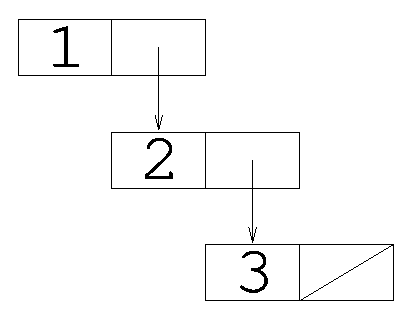
\epsfig{file=cons.ps}}
\end{center}
\end{figure}

List operations are typically implemented in a recursive fashion, where the cdr of the list is taken until the desired element is reached.

\wordtable{
\classword{general-list}{lists}\\
\classword{list}{lists}
}
A \emph{general list} is either the empty list or a cons cell. A \emph{list} is either the empty list or a cons cell whose cdr is also a list. A list is sometimes also known as a \emph{proper list}, and a general list that is not a proper list is known as a \texttt{improper list}. Not all list operations will function given an improper list,
however methods are usually defined on \texttt{general-list} not \texttt{list} since dispatching on \texttt{list} involves a costly check.

\subsubsection{List operations}

\wordtable{
\ordinaryword{>list}{>list ( sequence -- list )}{lists}
}
Turn an arbitrary sequence into a list.
\wordtable{
\ordinaryword{list?}{list?~( obj -- ?~)}{lists}
}
Tests if the object at the top of the stack is a proper list.
\wordtable{
\ordinaryword{unit}{unit ( obj -- [ obj ] )}{lists}
}
Makes a list of one element.
\wordtable{
\ordinaryword{2list}{2list ( o1 o2 -- [ o1 o2 ] )}{lists}
}
Makes a list of two elements.
\wordtable{
\ordinaryword{2unlist}{2unlist ( [ o1 o2 ] -- o1 o2 )}{lists}
}
Pushes the first two elements of a list.
\wordtable{
\ordinaryword{3list}{3list ( o1 o2 o3 -- [ o1 o2 o3 ] )}{lists}
}
Makes a list of three elements.
\wordtable{
\ordinaryword{3unlist}{3unlist ( [ o1 o2 o3 ] -- o1 o2 o3 )}{lists}
}
Pushes the first three elements of a list.
\wordtable{
\ordinaryword{unique}{unique ( obj list -- list )}{lists}
}
If the list already contains an element equal to the object, do nothing, otherwise cons the object into the list.
\wordtable{
\ordinaryword{prune}{prune ( list -- list )}{lists}
}
Removes all duplicates from the list by testing elements for equality.
\wordtable{
\ordinaryword{all=?}{all=?~( list -- ?~)}{lists}
}
Tests if all elements of the list are equal. For the empty list, this is vacuously true.
\wordtable{
\ordinaryword{head}{head~( list n -- list )}{lists}
}
Outputs a new list consisting of the first \texttt{n} elements of \texttt{list}. This allocates memory.
\wordtable{
\ordinaryword{tail}{tail~( list n -- list )}{lists}
}
Outputs a new list consisting of the elements of \texttt{list} from the $n$th index onward. This does not allocate memory; rather it simply takes the \texttt{cdr} \texttt{n} times.
\wordtable{
\ordinaryword{count}{count~( n -- list )}{lists}
}
Return a new list containing all integers from 0 up to $n-1$, inclusive.

\subsubsection{Set-theoretic operations}

\wordtable{
\ordinaryword{contains?}{contains?~( object list -- ?~)}{lists}
}
Tests if \texttt{list} contains an element equal to \texttt{object}.
\wordtable{
\ordinaryword{memq?}{memq?~( object list -- ?~)}{lists}
}
Tests if \texttt{list} contains \texttt{object}. Elements are compared by identity.
\wordtable{
\ordinaryword{contained?}{contained?~( l1 l2 -- ?~)}{lists}
}
Tests if every element of \texttt{l1} is equal to some element of \texttt{l2}.
\wordtable{
\ordinaryword{remove}{remove ( object list -- list )}{lists}
}
Outputs a new list containing all elements of the \texttt{list} except those equal to the \texttt{object}.
\wordtable{
\ordinaryword{remq}{remove ( object list -- list )}{lists}
}
Outputs a new list containing all elements of the \texttt{list} except \texttt{object}. Elements are compared by identity.
\wordtable{
\ordinaryword{intersection}{intersection ( list list -- list )}{lists}
}
Outputs a list of elements present in both lists.
\wordtable{
\ordinaryword{intersection}{difference ( l1 l2 -- list )}{lists}
}
Outputs a list of elements present in \texttt{l2} but not \texttt{l1}.

\subsubsection{List combinators}

\wordtable{
\ordinaryword{each}{each ( list quot -- )}{lists}\\
\texttt{quot:~element --}
}
Applies the quotation to each element of the list.
\wordtable{
\ordinaryword{map}{map ( list quot -- list )}{lists}\\
\texttt{quot:~element -- element}
}
Applies the quotation to each element yielding a new element. The new elements are collected into a new list.
\wordtable{
\ordinaryword{subset}{subset ( list quot -- list )}{lists}\\
\texttt{quot:~element -- ?}
}
Applies the quotation to each element, and outputs a new list containing the elements of the original list for which the quotation output true.
\wordtable{
\ordinaryword{some?}{some?~( list quot -- list )}{lists}\\
\texttt{quot:~element -- ?}
}
Applies the quotation to each element, and outputs the rest of the list upon encountering an element for which the quotation outputs true. If the quotation did not output true for any element, \texttt{some?}~outputs \texttt{f}. Note that the output is a generalized boolean; if the quotation matched any element, the result is true.
\wordtable{
\ordinaryword{all?}{all?~( list quot -- list )}{lists}\\
\texttt{quot:~element -- ?}
}
Outputs \texttt{t} if the quotation yields true when applied to each element, otherwise outputs \texttt{f}. Given the empty list, vacuously outputs \texttt{t}.
\wordtable{
\ordinaryword{sort}{all?~( list quot -- list )}{lists}\\
\texttt{quot:~e1 e2 -- ?}
}
Sorts the list by comparing each pair of elements with the quotation. The quotation should output \texttt{t} if \texttt{e2} is to come before \texttt{e1} in the list. For example, to sort a list of numbers in ascending order, you can do the following:
\begin{alltt}
\textbf{ok} [ 8 6 9 1 10 3 ] [ > ] sort .
[ 1 3 6 8 9 10 ]
\end{alltt}
\wordtable{
\ordinaryword{each-with}{each-with ( object list quot -- )}{lists}\\
\texttt{quot:~object element --}\\
\ordinaryword{map-with}{map-with ( object list quot -- list )}{lists}\\
\texttt{quot:~object element -- element}\\
\ordinaryword{subset-with}{subset-with ( object list quot -- list )}{lists}\\
\texttt{quot:~object element -- ?}\\
\ordinaryword{some-with?}{some-with?~( object list quot -- ?~)}{lists}\\
\texttt{quot:~object element -- ?}\\
\ordinaryword{all-with?}{all-with?~( object list quot -- ?~)}{lists}\\
\texttt{quot:~object element -- ?}
}
Curried forms of the above combinators. They pass an additional object to each invocation of the quotation.

\subsubsection{Queues}

The following set of words manages LIFO (last-in-first-out) queues. Queues are built up from cons cells, and hence are immutable; queue operations always return a new queue.

\wordtable{
\ordinaryword{<queue>}{<queue> ( -- queue )}{lists}
}
Makes a new queue with no elements.
\wordtable{
\ordinaryword{queue-empty?}{queue-empty? ( queue -- ?~)}{lists}
}
Outputs \texttt{t} if the given queue does not contain any elements, \texttt{f} otherwise.
\wordtable{
\ordinaryword{deque}{deque ( queue -- element queue )}{lists}
}
Dequeues an element and outputs a new queue without that element.
\wordtable{
\ordinaryword{enque}{deque ( element queue -- queue )}{lists}
}
Enqueues an element and outputs a new queue.

\subsection{Strings}

\stringglos
\wordtable{
\classword{string}{strings}
}
A string is an immutable sequence of characters. The literal syntax is covered in \ref{string-literals}. Characters do not have a distinct data type, so elements taken out of strings appear as integers on the stack.

\wordtable{
\ordinaryword{string?}{string?~( obj -- ?~)}{strings}
}
Tests if the object at the top of the stack is a string.
%\wordtable{
%\ordinaryword{>string}{>string~( sequence -- string )}{strings}
%}
%Turns any type of sequence with all-integer elements into a string. The integer elements are interpreted as characters.
\wordtable{
\ordinaryword{string-compare}{string-compare~( s1 s2 -- n )}{strings}
}
Compare two strings lexicographically (dictionary order). The output value is one of the following:
\begin{description}
\item[Positive] indicating that \texttt{s1} follows \texttt{s2}
\item[Zero] indicating that \texttt{s1} is equal to \texttt{s2}
\item[Negative] indicating that \texttt{s1} precedes \texttt{s2}
\end{description}
\wordtable{
\ordinaryword{string>}{string> ( s1 s2 -- ?~)}{strings}
}
Tests if \texttt{s1} follows \texttt{s2}. Implemented as follows:
\begin{verbatim}
: string> ( s1 s1 -- ? ) string-compare 0 > ;
\end{verbatim}
This is used to sort lists of strings:
\begin{alltt}
\textbf{ok} [ "Curry" "Apple" "Veal" "Turkey" ] [ string> ] sort .
[ "Apple" "Curry" "Turkey" "Veal" ]
\end{alltt}
\wordtable{
\ordinaryword{fill}{fill~( n char -- string )}{strings}
}
Creates a string with \texttt{char} repeated $n$ times.
\wordtable{
\ordinaryword{pad}{pad~( string n char -- string )}{strings}
}
Creates a string with \texttt{char} repeated $l-n$ times, where $l$ is the length of \texttt{string}. If $l$ is greater than $n$, the empty string is output.

\subsubsection{Substring testing}

\wordtable{
\ordinaryword{string-contains?}{string-contains?~( s1 s2 -- ?~)}{strings}
}
Tests if \texttt{s2} contains \texttt{s1} as a substring.
\wordtable{
\ordinaryword{string-head?}{string-head?~( s1 s2 -- ?~)}{strings}\\
\ordinaryword{string-tail?}{string-tail?~( s1 s2 -- ?~)}{strings}
}
Tests if \texttt{s1} starts or ends with \texttt{s1} as a substring. If \texttt{s1} is longer than \texttt{s2}, outputs \texttt{f}.

\subsubsection{Slicing and splitting}

\wordtable{
\ordinaryword{string/}{string/ ( string n -- s1 s2 )}{strings}
}
Outputs a pair of strings that equal the original string when concatenated. The first string has length $n$, the second has length $l-n$ where $l$ is the length of the input.
\begin{alltt}
\textbf{ok} "Hello world" 5 string .s
\textbf{" world"
"Hello"}
\end{alltt}
\wordtable{
\ordinaryword{string//}{string// ( string n -- s1 s2 )}{strings}
}

Outputs a pair of strings that equal the original string, excluding the $n$th element, when concatenated. The first string has length $n$, the second has length $l-n$ where $l$ is the length of the input.
\begin{alltt}
\textbf{ok} "Hello world" 5 string// .s
\textbf{"world"
"Hello"}
\end{alltt}
\wordtable{
\ordinaryword{?string-head}{?string-head~( s1 s2 -- string ?~)}{strings}\\
\ordinaryword{?string-tail}{?string-tail~( s1 s2 -- string ?~)}{strings}
}
Tests if \texttt{s1} starts or ends with \texttt{s1} as a substring. If there is a match, outputs the subrange of \texttt{s1} excluding \texttt{s1} followed by \texttt{t}. If there is no match, outputs \texttt{s1} followed by \texttt{f}/
\wordtable{
\ordinaryword{split1}{split1~( str split -- before after )}{strings}
}
If \texttt{string} does not contain \texttt{split} as a substring, then \texttt{before} is equal to the \texttt{string}, and \texttt{after} is \texttt{f}. Otherwise, \texttt{before} and \texttt{after} are both strings, and yield the input excluding \texttt{split} when concatenated.
\wordtable{
\ordinaryword{split}{split~( str split -- list )}{strings}
}
Outputs a list of substrings taken between occurrences of \texttt{split} in \texttt{string}. If \texttt{split} does not occur inside \texttt{string}, outputs a singleton list containing \texttt{string} only.
\begin{alltt}
\textbf{ok} "/usr/local/bin" CHAR: / split .
\textbf{[ "" "usr" "local" "bin" ]}
\end{alltt}
\wordtable{
\ordinaryword{split-n}{split-n~( str n -- list )}{strings}
}
Splits the string into groups of \texttt{n} characters and collects them in a list. If the string's length is not a multiple of \texttt{n}, the final string in the list might be shorter.

\subsubsection{Characters}

\wordtable{
\ordinaryword{ch>string}{ch>string ( n -- string )}{strings}
}
Turns an integer representing a character value into a single-element string.
\wordtable{
\ordinaryword{blank?}{blank?~( n -- ?~)}{strings}\\
\ordinaryword{letter?}{letter?~( n -- ?~)}{strings}\\
\ordinaryword{LETTER?}{LETTER?~( n -- ?~)}{strings}\\
\ordinaryword{digit?}{digit?~( n -- ?~)}{strings}\\
\ordinaryword{printable?}{printable?~( n -- ?~)}{strings}\\
\ordinaryword{quotable?}{quotable?~( n -- ?~)}{strings}\\
\ordinaryword{url-quotable?}{url-quotable?~( n -- ?~)}{strings}
}
Various character classification predicates.

\subsection{String buffers}

\sbufglos
\wordtable{
\classword{sbuf}{strings}
}
A string buffer is a mutable and growable sequence of characters. String buffers can be used to construct new strings by accumilating substrings and characters, however usually they are only used indirectly, since the sequence construction words in \ref{make-seq} are more convenient to use in many cases.
\wordtable{
\ordinaryword{sbuf?}{sbuf?~( object -- ?~)}{strings}
}
Tests if the object at the top of the stack is a string buffer.
\wordtable{
\ordinaryword{>sbuf}{>sbuf~( sequence -- sbuf )}{strings}
}
Turns any type of sequence into a string buffer. Given a string buffer, this makes a fresh copy
\wordtable{
\ordinaryword{sbuf>string}{sbuf>string~( sbuf -- string )}{strings}
}
Turns a string buffer into a string holding the same characters.

\subsection{\label{make-seq}Constructing sequences}

The library supports an idiom where sequences can be constructed without passing the partial sequence being built on the stack. This reduces stack noise, and thus simplifies code and makes it easier to understand.

\newcommand{\dynamicscopeglos}{\glossary{
name=dynamic scope,
description={a variable binding policy where bindings established in a scope are visible to all code executed while the scope is active}}}
\dynamicscopeglos
\wordtable{
\ordinaryword{make-list}{make-list ( quot -- list )}{namespaces}\\
\ordinaryword{make-string}{make-string ( quot -- string )}{namespaces}\\
\ordinaryword{make-sbuf}{make-sbuf ( quot -- string )}{namespaces}\\
\ordinaryword{make-vector}{make-vector ( quot -- vector )}{namespaces}
}
Calls the quotation in a new \texttt{dynamic scope}. The quotation and any words it calls can execute the \texttt{,} and \texttt{\%} words to add elements at the end of the sequence being constructed.
\wordtable{
\ordinaryword{,}{,~( element -- )}{namespaces}
}
Adds the element to the end of the sequence being constructed by the innermost call to one of the above combinators.
\wordtable{
\ordinaryword{unique,}{unique,~( element -- )}{namespaces}
}
Adds the element to the end of the sequence being constructed as long as the sequence does not already have an equal element.
\wordtable{
\ordinaryword{literal,}{literal,~( element -- )}{namespaces}
}
Adds the element wrapped inside a one-element list, then adds the \texttt{car} word. This is used to construct quotations with \texttt{make-list} that must push a word on the stack.
\wordtable{
\ordinaryword{\%}{\% ( sequence -- )}{namespaces}
}
Appends the subsequence to the end of the sequence being constructed.

Note that the sequence construction combinators will capture any variables set inside the quotation, due to the dynamic scoping behavior. These combinators are actually implemented using variables. See \ref{namespaces}.

\section{Mappings}

\glossary{name=mapping,
description={an unordered collection of elements, accessed by key. Examples include association lists and hashtables}}

Mappings associate keys with values. The two classes of mappings in the Factor library are association lists and hashtables.

\begin{tabular}[t]{l|c|c|c|l}
Class&Mutable&Ordered&Lookup&Primary purpose\\
\hline
\texttt{assoc}&&$\surd$&$O(n)$&Small, unchanging mappings\\
\texttt{hashtable}&$\surd$&&$O(1)$&Large or frequently-changing mappings
\end{tabular}

It might be tempting to just always use hashtables, however for very small mappings, association lists are just as efficient, and are easier to work with since the entire set of list words can be used with them.

\subsection{Association lists}

\glossary{name=association list,
description={a list of pairs, where the car if each pair is a key and the cdr is the value associated with that key}}

Association lists are built from cons cells. They are structured like a ribbed spine, where the ``spine'' is a list and each ``rib'' is a cons cell holding a key/value pair.

\wordtable{
\ordinaryword{assoc?}{assoc ( object -- ?~)}{lists}
}
Tests if the object at the top of the stack is a proper list whose every element is a cons.

\wordtable{
\ordinaryword{assoc}{assoc ( k alist -- v )}{lists}\\
\ordinaryword{assoc*}{assoc* ( k alist -- [[ k v ]] )}{lists}
}
These words look up a key in an association list, comparing keys in the list with the given key by equality with \texttt{=}. The list is searched starting from the beginning. The two words differ in that the latter returns the key/value pair located, whereas the former only returns the value. The \texttt{assoc*} word allows a distinction to be made between a missing value and a value equal to \texttt{f}, since in the case of a missing value it outputs \texttt{f}.
\wordtable{
\ordinaryword{assq}{assq ( k alist -- v )}{lists}\\
\ordinaryword{assq*}{assq* ( k alist -- [[ k v ]] )}{lists}
}
These words compare keys by identity with \texttt{eq?}~and are dual to \texttt{assoc} and \texttt{assoc*}.
\wordtable{
\ordinaryword{acons}{acons ( v k alist -- alist )}{lists}\\
\ordinaryword{set-assoc}{set-assoc ( v k alist -- alist )}{lists}
}
These words output a new association list containing the key/value pair.
They differ in that \texttt{set-assoc} removes any existing key/value pairs with the given key first. In both cases, searching for the key in the returned association list gives the new value, however with the slightly faster \texttt{acons}, the old value remains shadowed in the list.
\wordtable{
\ordinaryword{remove-assoc}{remove-assoc ( k alist -- alist )}{lists}
}
Outputs a new association list which does not have any key/value pairs with the key equal to \texttt{k}.

\begin{figure}
\caption{An association list and its graphical representation}
\begin{verbatim}
[
    [[ "Salsa" "Hot" ]]
    [[ "Stir-Fry" "Medium" ]]
    [[ "Peppers" "Very Hot" ]]
]
\end{verbatim}

\begin{center}
\scalebox{0.45}{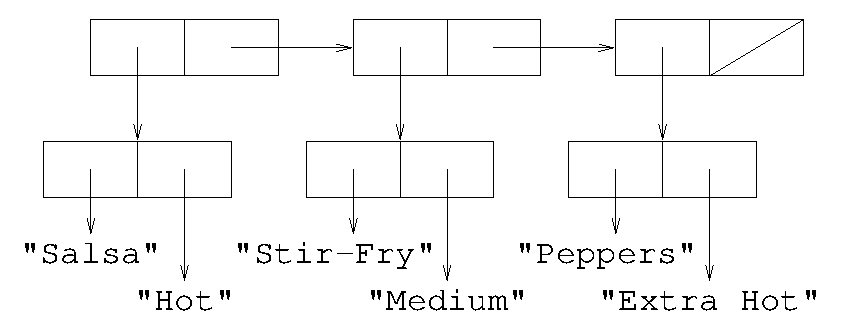
\epsfig{file=assoc.eps}}
\end{center}
\end{figure}

\subsubsection{Dual representation}

Sometimes it is convenient to decompose an association list into two lists of equal length, containing the keys and values, respectively, in the same order as the association list. This dual representation can be manipulated with a handful of helper words.

\wordtable{
\ordinaryword{zip}{zip ( keys values -- alist )}{lists}\\
\ordinaryword{unzip}{unzip ( alist -- keys values )}{lists}
}
These words convert between pairs of lists and lists of pairs.
\begin{alltt}
\textbf{ok} [ 1 2 3 ] [ 4 5 6 ] zip .
[ [[ 1 4 ]] [[ 2 5 ]] [[ 3 6 ]] ]
\textbf{ok} [ [[ 1 2 ]] [[ 3 4 ]] [[ 5 6 ]] ] unzip .s
[ 2 4 6 ]
[ 1 3 5 ]
\end{alltt}
\wordtable{
\ordinaryword{2cons}{2cons ( car1 car2 cdr1 cdr2 -- c1 c2 )}{lists}
}
Cons a pair of elements onto a pair of lists.
\wordtable{
\ordinaryword{2car}{2car ( c1 c2 -- car1 car2 )}{lists}\\
\ordinaryword{2cdr}{2cdr ( c1 c2 -- cdr1 cdr2 )}{lists}
}
Deconstructs paired lists.

\subsection{Hashtables}

\wordtable{
\classword{hashtable}{hashtables}
}


\subsection{\label{namespaces}Namespaces}

\section{Mathematics}

\numberglos

\begin{figure}
\begin{center}
\caption{Numerical class hierarchy}
\scalebox{0.5}{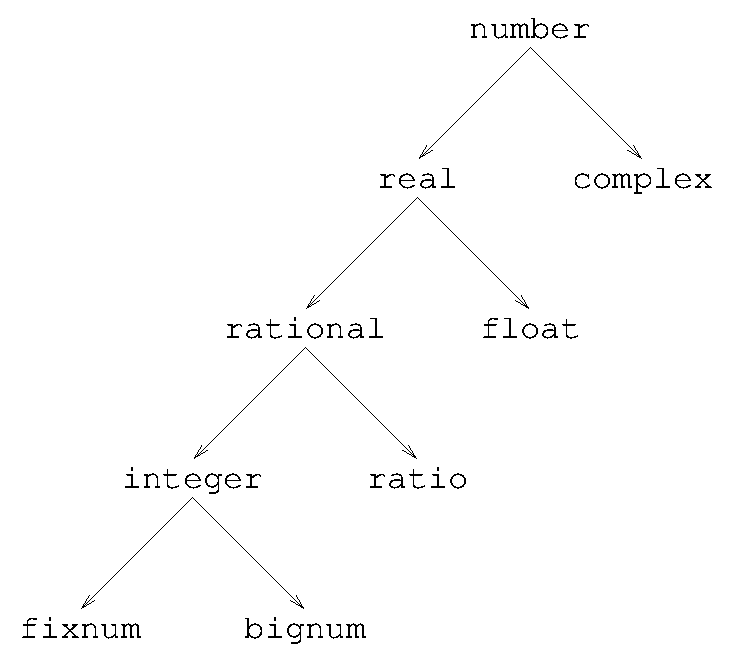
\epsfig{file=number.ps}}
\end{center}
\end{figure}

Factor's numbers more closely model the mathematical concept of a number than other languages. Where possible, exact answers are given -- for example, adding or multiplying two integers never results in overflow, and dividing two integers yields a fraction rather than a truncated result. Complex numbers are supported, allowing many functions to be computed with parameters that would raise errors or return ``not a number'' in other languages.

\subsection{Integers}

\integerglos

The simplest type of number is the integer. Integers come in two varieties -- \emph{fixnums} and \emph{bignums}. As their names suggest, a fixnum is a fixed-width quantity\footnote{Fixnums range in size from $-2^{w-3}-1$ to $2^{w-3}$, where $w$ is the word size of your processor (for example, 32 bits). Because fixnums automatically grow to bignums, usually you do not have to worry about details like this.}, and is a bit quicker to manipulate than an arbitrary-precision bignum.

The predicate word \texttt{integer?}~tests if the top of the stack is an integer. If this returns true, then exactly one of \texttt{fixnum?}~or \texttt{bignum?}~would return true for that object. Usually, your code does not have to worry if it is dealing with fixnums or bignums.

Unlike some languages where the programmer has to declare storage size explicitly and worry about overflow, integer operations automatically return bignums if the result would be too big to fit in a fixnum. Here is an example where multiplying two fixnums returns a bignum:

\begin{alltt}
\textbf{ok} 134217728 fixnum? .
\textbf{t}
\textbf{ok} 128 fixnum? .
\textbf{t}
\textbf{ok} 134217728 128 * .
\textbf{17179869184}
\textbf{ok} 134217728 128 * bignum? .
\textbf{t}
\end{alltt}

Integers can be entered using a different base. By default, all number entry is in base 10, however this can be changed by prefixing integer literals with one of the parsing words \texttt{BIN:}, \texttt{OCT:}, or \texttt{HEX:}. For example:

\begin{alltt}
\textbf{ok} BIN: 1110 BIN: 1 + .
\textbf{15}
\textbf{ok} HEX: deadbeef 2 * .
\textbf{7471857118}
\end{alltt}

The word \texttt{.} prints numbers in decimal, regardless of how they were input. A set of words in the \texttt{prettyprint} vocabulary is provided for print integers using another base.

\begin{alltt}
\textbf{ok} 1234 .h
\textbf{4d2}
\textbf{ok} 1234 .o
\textbf{2232}
\textbf{ok} 1234 .b
\textbf{10011010010}
\end{alltt}

\subsection{Rational numbers}

\newcommand{\rationalglos}{\glossary{
name=rational,
description={an instance of the \texttt{rational} class, which is a disjoint union of the
\texttt{integer} and \texttt{ratio} classes}}}
\rationalglos
\ratioglos

If we add, subtract or multiply any two integers, the result is always an integer. However, this is not the case with division. When dividing a numerator by a denominator where the numerator is not a integer multiple of the denominator, a ratio is returned instead.

\begin{alltt}
1210 11 / .
\emph{110}
100 330 / .
\emph{10/33}
\end{alltt}

Ratios are printed and can be input literally in the form of the second example. Ratios are always reduced to lowest terms by factoring out the greatest common divisor of the numerator and denominator. A ratio with a denominator of 1 becomes an integer. Trying to create a ratio with a denominator of 0 raises an error.

The predicate word \texttt{ratio?}~tests if the top of the stack is a ratio. The predicate word \texttt{rational?}~returns true if and only if one of \texttt{integer?}~or \texttt{ratio?}~would return true for that object. So in Factor terms, a ``ratio'' is a rational number whose denominator is not equal to 1.

Ratios behave just like any other number -- all numerical operations work as expected, and in fact they use the formulas for adding, subtracting and multiplying fractions that you learned in high school.

\begin{alltt}
\textbf{ok} 1/2 1/3 + .
\textbf{5/6}
\textbf{ok} 100 6 / 3 * .
\textbf{50}
\end{alltt}

Ratios can be deconstructed into their numerator and denominator components using the \texttt{numerator} and \texttt{denominator} words. The numerator and denominator are both integers, and furthermore the denominator is always positive. When applied to integers, the numerator is the integer itself, and the denominator is 1.

\begin{alltt}
\textbf{ok} 75/33 numerator .
\textbf{25}
\textbf{ok} 75/33 denominator .
\textbf{11}
\textbf{ok} 12 numerator .
\textbf{12}
\end{alltt}

\subsection{Floating point numbers}

\newcommand{\realglos}{\glossary{
name=real,
description={an instance of the \texttt{real} class, which is a disjoint union of the
\texttt{rational} and \texttt{float} classes}}}
\realglos
\floatglos

Rational numbers represent \emph{exact} quantities. On the other hand, a floating point number is an \emph{approximation}. While rationals can grow to any required precision, floating point numbers are fixed-width, and manipulating them is usually faster than manipulating ratios or bignums (but slower than manipulating fixnums). Floating point literals are often used to represent irrational numbers, which have no exact representation as a ratio of two integers. Floating point literals are input with a decimal point.

\begin{alltt}
\textbf{ok} 1.23 1.5 + .
\textbf{1.73}
\end{alltt}

The predicate word \texttt{float?}~tests if the top of the stack is a floating point number. The predicate word \texttt{real?}~returns true if and only if one of \texttt{rational?}~or \texttt{float?}~would return true for that object.

Floating point numbers are \emph{contagious} -- introducing a floating point number in a computation ensures the result is also floating point.

\begin{alltt}
\textbf{ok} 5/4 1/2 + .
\textbf{7/4}
\textbf{ok} 5/4 0.5 + .
\textbf{1.75}
\end{alltt}

Apart from contaigion, there are two ways of obtaining a floating point result from a computation; the word \texttt{>float ( n -{}- f )} converts a rational number into its floating point approximation, and the word \texttt{/f ( x y -{}- x/y )} returns the floating point approximation of a quotient of two numbers.

\begin{alltt}
\textbf{ok} 7 4 / >float .
\textbf{1.75}
\textbf{ok} 7 4 /f .
\textbf{1.75}
\end{alltt}

Indeed, the word \texttt{/f} could be defined as follows:

\begin{alltt}
: /f / >float ;
\end{alltt}

However, the actual definition is slightly more efficient, since it computes the floating point result directly.

\subsection{Complex numbers}

Complex numbers arise as solutions to quadratic equations whose graph does not intersect the x axis. For example, the equation $x^2 + 1 = 0$ has no solution for real $x$, because there is no real number that is a square root of -1. However, in the field of complex numbers, this equation has a well-known solution:

\begin{alltt}
\textbf{ok} -1 sqrt .
\textbf{\#\{ 0 1 \}}
\end{alltt}

The literal syntax for a complex number is \texttt{\#\{ re im \}}, where \texttt{re} is the real part and \texttt{im} is the imaginary part. For example, the literal \texttt{\#\{ 1/2 1/3 \}} corresponds to the complex number $1/2 + 1/3i$.

The words \texttt{i} an \texttt{-i} push the literals \texttt{\#\{ 0 1 \}} and \texttt{\#\{ 0 -1 \}}, respectively.

The predicate word \texttt{complex?} tests if the top of the stack is a complex number. Note that unlike math, where all real numbers are also complex numbers, Factor only considers a number to be a complex number if its imaginary part is non-zero.

Complex numbers can be deconstructed into their real and imaginary components using the \texttt{real} and \texttt{imaginary} words. Both components can be pushed at once using the word \texttt{>rect ( z -{}- re im )}.

\begin{alltt}
\textbf{ok} -1 sqrt real .
\textbf{0}
\textbf{ok} -1 sqrt imaginary .
\textbf{1}
\textbf{ok} -1 sqrt sqrt >rect .s
\textbf{\{ 0.7071067811865476 0.7071067811865475 \}}
\end{alltt}

A complex number can be constructed from a real and imaginary component on the stack using the word \texttt{rect> ( re im -{}- z )}.

\begin{alltt}
\textbf{ok} 1/3 5 rect> .
\textbf{\#\{ 1/3 5 \}}
\end{alltt}

Complex numbers are stored in \emph{rectangular form} as a real/imaginary component pair (this is where the names \texttt{>rect} and \texttt{rect>} come from). An alternative complex number representation is \emph{polar form}, consisting of an absolute value and argument. The absolute value and argument can be computed using the words \texttt{abs} and \texttt{arg}, and both can be pushed at once using \texttt{>polar ( z -{}- abs arg )}.

\begin{alltt}
\textbf{ok} 5.3 abs .
\textbf{5.3}
\textbf{ok} i arg .
\textbf{1.570796326794897}
\textbf{ok} \#\{ 4 5 \} >polar .s
\textbf{\{ 6.403124237432849 0.8960553845713439 \}}
\end{alltt}

A new complex number can be created from an absolute value and argument using \texttt{polar> ( abs arg -{}- z )}.

\begin{alltt}
\textbf{ok} 1 pi polar> .
\textbf{\#\{ -1.0 1.224606353822377e-16 \}}
\end{alltt}

\subsection{Transcedential functions}

The \texttt{math} vocabulary provides a rich library of mathematical functions that covers exponentiation, logarithms, trigonometry, and hyperbolic functions. All functions accept and return complex number arguments where appropriate. These functions all return floating point values, or complex numbers whose real and imaginary components are floating point values.

\texttt{\^{} ( x y -- x\^{}y )} raises \texttt{x} to the power of \texttt{y}. In the cases of \texttt{y} being equal to $1/2$, -1, or 2, respectively, the words \texttt{sqrt}, \texttt{recip} and \texttt{sq} can be used instead.

\begin{alltt}
\textbf{ok} 2 4 \^ .
\textbf{16.0}
\textbf{ok} i i \^ .
\textbf{0.2078795763507619}
\end{alltt}

All remaining functions have a stack effect \texttt{( x -{}- y )}, it won't be repeated for brevity.

\texttt{exp} raises the number $e$ to a specified power. The number $e$ can be pushed on the stack with the \texttt{e} word, so \texttt{exp} could have been defined as follows:

\begin{alltt}
: exp ( x -- e^x ) e swap \^ ;
\end{alltt}

However, it is actually defined otherwise, for efficiency.\footnote{In fact, the word \texttt{\^{}} is actually defined in terms of \texttt{exp}, to correctly handle complex number arguments.}

\texttt{log} computes the natural (base $e$) logarithm. This is the inverse of the \texttt{exp} function.

\begin{alltt}
\textbf{ok} -1 log .
\textbf{\#\{ 0.0 3.141592653589793 \}}
\textbf{ok} e log .
\textbf{1.0}
\end{alltt}

\texttt{sin}, \texttt{cos} and \texttt{tan} are the familiar trigonometric functions, and \texttt{asin}, \texttt{acos} and \texttt{atan} are their inverses.

The reciprocals of the sine, cosine and tangent are defined as \texttt{sec}, \texttt{cosec} and \texttt{cot}, respectively. Their inverses are \texttt{asec}, \texttt{acosec} and \texttt{acot}.

\texttt{sinh}, \texttt{cosh} and \texttt{tanh} are the hyperbolic functions, and \texttt{asinh}, \texttt{acosh} and \texttt{atanh} are their inverses.

Similarly, the reciprocals of the hyperbolic functions are defined as \texttt{sech}, \texttt{cosech} and \texttt{coth}, respectively. Their inverses are \texttt{asech}, \texttt{acosech} and \texttt{acoth}.

\subsection{Modular arithmetic}

In addition to the standard division operator \texttt{/}, there are a few related functions that are useful when working with integers.

\texttt{/i ( x y -{}- x/y )} performs a truncating integer division. It could have been defined as follows:

\begin{alltt}
: /i / >integer ;
\end{alltt}

However, the actual definition is a bit more efficient than that.

\texttt{mod ( x y -{}- x\%y )} computes the remainder of dividing \texttt{x} by \texttt{y}. If the result is 0, then \texttt{x} is a multiple of \texttt{y}.

\texttt{/mod ( x y -{}- x/y x\%y )} pushes both the quotient and remainder.

\begin{alltt}
\textbf{ok} 100 3 mod .
\textbf{1}
\textbf{ok} -546 34 mod .
\textbf{-2}
\end{alltt}

\texttt{gcd ( x y -{}- z )} pushes the greatest common divisor of two integers; that is, the largest number that both integers could be divided by and still yield integers as results. This word is used behind the scenes to reduce rational numbers to lowest terms when doing ratio arithmetic.

\subsection{Bitwise operations}

There are two ways of looking at an integer -- as a mathematical entity, or as a string of bits. The latter representation faciliates the so-called \emph{bitwise operations}.

\texttt{bitand ( x y -{}- x\&y )} returns a new integer where each bit is set if and only if the corresponding bit is set in both $x$ and $y$. If you're considering an integer as a sequence of bit flags, taking the bitwise-and with a mask switches off all flags that are not explicitly set in the mask.

\begin{alltt}
BIN: 101 BIN: 10 bitand .b
\emph{0}
BIN: 110 BIN: 10 bitand .b
\emph{10}
\end{alltt}

\texttt{bitor ( x y -{}- x|y )} returns a new integer where each bit is set if and only if the corresponding bit is set in at least one of $x$ or $y$. If you're considering an integer as a sequence of bit flags, taking the bitwise-or with a mask switches on all flags that are set in the mask.

\begin{alltt}
BIN: 101 BIN: 10 bitor .b
\emph{111}
BIN: 110 BIN: 10 bitor .b
\emph{110}
\end{alltt}

\texttt{bitxor ( x y -{}- x\^{}y )} returns a new integer where each bit is set if and only if the corresponding bit is set in exactly one of $x$ or $y$. If you're considering an integer as a sequence of bit flags, taking the bitwise-xor with a mask toggles on all flags that are set in the mask.

\begin{alltt}
BIN: 101 BIN: 10 bitxor .b
\emph{111}
BIN: 110 BIN: 10 bitxor .b
\emph{100}
\end{alltt}

\texttt{bitnot ( x -{}- y )} returns the bitwise complement of the input; that is, each bit in the input number is flipped. This is actually equivalent to negating a number, and subtracting one. So indeed, \texttt{bitnot} could have been defined as thus:

\begin{alltt}
: bitnot neg pred ;
\end{alltt}

\texttt{shift ( x n -{}- y )} returns a new integer consisting of the bits of the first integer, shifted to the left by $n$ positions. If $n$ is negative, the bits are shifted to the right instead, and bits that ``fall off'' are discarded.

\begin{alltt}
BIN: 101 5 shift .b
\emph{10100000}
BIN: 11111 -2 shift .b
\emph{111}
\end{alltt}

The attentive reader will notice that shifting to the left is equivalent to multiplying by a power of two, and shifting to the right is equivalent to performing a truncating division by a power of two.

\chapter{The development environment}

Factor supports interactive development in a live environment. Instead of working with
static executable files and restarting your application after each change, you can
incrementally make changes to your application and test them immediately. If you
notice an undesirable behavior, Factor's powerful reflection features will aid in
pinpointing the error.

If you are used to a statically typed language, you might find Factor's tendency to only fail at runtime hard to work with at first. However, the interactive development tools outlined in this document allow a much quicker turn-around time for testing changes. Also, write unit tests -- unit testing is a great way to ensure that old bugs do not re-appear once they've been fixed.

\section{System organization}

\subsection{The listener}

Factor is an \emph{image-based environment}. When you compiled Factor, you also generated a file named \texttt{factor.image}. I will have more to say about images later, but for now it suffices to understand that to start Factor, you must pass the image file name on the command line:
\begin{alltt}
./f factor.image
\textbf{Loading factor.image... relocating... done
Factor 0.73 :: http://factor.sourceforge.net :: unix/x86
(C) 2003, 2005 Slava Pestov, Chris Double,
Mackenzie Straight
ok}
\end{alltt}
An \texttt{\textbf{ok}} prompt is printed after the initial banner, indicating the listener is ready to execute Factor phrases. The listener is a piece of Factor code, like any other; however, it helps to think of it as the primary interface to the Factor system. The listener reads Factor code and executes it. You can try the classical first program:

\begin{alltt}
\textbf{ok} "Hello, world." print
\textbf{Hello, world.}
\end{alltt}


Multi-line phrases are supported; if there are unclosed brackets, the listener outputs \texttt{...} instead of the \texttt{ok} prompt, and the entire phrase is executed once all brackets are closed:

\begin{alltt}
\textbf{ok} [ 1 2 3 ] [
\textbf{...} .
\textbf{...} ] each
\textbf{1
2
3}
\end{alltt}

The listener knows when to print a continuation prompt by looking at the height of the
stack. Parsing words such as \texttt{[} and \texttt{:} leave elements on the parser
stack; these elements are popped by \texttt{]} and \texttt{;}.

\subsection{Source files}

While it is possible to do all development in the listener and save your work in images, it is far more convenient to work with source files, at least until an in-image structure editor is developed.

By convention, Factor source files are saved with the \texttt{.factor} filename extension. They can be loaded into the image as follows:

\begin{alltt}
\textbf{ok} "examples/numbers-game.factor" run-file
\end{alltt}

In Factor, loading a source file replaces any existing definitions\footnote{But see \ref{compiler} for this is not true of compiled code.}. Each word definition remembers what source file it was loaded from (if any). To reload the source file associated with a definition, use the \texttt{reload} word:

\begin{alltt}
\textbf{ok} \bs draw reload
\end{alltt}

Word definitions also retain the line number where they are located in their original source file. This allows you to open a word definition in jEdit\footnote{\texttt{http://www.jedit.org}} for editing using the
\texttt{jedit} word:

\begin{alltt}
\textbf{ok} \bs compile jedit
\end{alltt}

This word requires that a jEdit instance is already running.

For the \texttt{jedit} word to work with words in the Factor library, you must set the \texttt{"resource-path"} variable to the location of the Factor source tree. One way to do this is to add a phrase like the following to your \texttt{.factor-rc}:

\begin{verbatim}
"/home/slava/Factor/" "resource-path" set
\end{verbatim}

On startup, Factor reads the \texttt{.factor-rc} file from your home directory. You can put
any quick definitions you want available at the listener there. To avoid loading this
file, pass the \texttt{-no-user-init} command line switch. Another way to have a set of definitions available at all times is to save a custom image, as described in the next section.

\subsection{Images}

The \texttt{factor.image} file is basically a dump of all objects in the heap. A new image can be saved as follows:

\begin{alltt}
\textbf{ok} "work.image" save-image
\textbf{Saving work.image...}
\end{alltt}

When you save an image before exiting Factor, then start Factor again, everything will be almost as you left it. Try the following:

\begin{alltt}
./f factor.image
\textbf{ok} "Learn Factor" "reminder" set
\textbf{ok} "factor.image" save-image bye
\textbf{Saving factor.image...}
\end{alltt}

Factor will save the image and exit. Now start it again and see that the reminder is still there:

\begin{alltt}
./f factor.image
\textbf{ok} "reminder" get .
\textbf{"Learn Factor"}
\end{alltt}

This is what is meant by the image being an \emph{infinite session}. When you shut down and restart Factor, what happends is much closer to a Laptop's ``suspend'' mode, than a desktop computer being fully shut down.

\subsection{Looking at objects}

Probably the most important debugging tool of them all is the \texttt{.} word. It prints the object at the top of the stack in a form that can be parsed by the Factor parser. A related word is \texttt{prettyprint}. It is identical to \texttt{.} except the output is more verbose; lists, vectors and hashtables are broken up into multiple lines and indented.

\begin{alltt}
\textbf{ok} [ [ \tto 1 \ttc \tto 2 \ttc ] dup car swap cdr ] .
[ [ \tto 1 \ttc \tto 2 \ttc ] dup car swap cdr ]
\end{alltt}

Most objects print in a parsable form, but not all. One exceptions to this rule is objects with external state, such as I/O ports or aliens (pointers to native structures). Also, objects with circular or very deeply nested structure will not print in a fully parsable form, since the prettyprinter has a limit on maximum nesting. Here is an example -- a vector is created, that holds a list whose first element is the vector itself:

\begin{alltt}
\textbf{ok} \tto \ttc [ unit 0 ] keep [ set-vector-nth ] keep .
\tto [ ... ] \ttc
\end{alltt}

The prettyprinted form of a vector or list with many elements is not always readable. The \texttt{[.]} and \texttt{\tto.\ttc} words output a list or a vector, respectively, with each element on its own line. In fact, the stack printing words are defined in terms of \texttt{[.]} and \texttt{\tto.\ttc}:

\begin{verbatim}
: .s datastack  {.} ;
: .r callstack  {.} ;
: .n namestack  [.] ;
: .c catchstack [.] ;
\end{verbatim}

Before we move on, one final set of output words comes is used to output integers in
different numeric bases. The \texttt{.b} word prints an integer in binary, \texttt{.o} in octal, and \texttt{.h} in hexadecimal.

\begin{alltt}
\textbf{ok} 31337 .b
\textbf{111101001101001}
\textbf{ok} 31337 .o
\textbf{75151}
\textbf{ok} 31337 .h
\textbf{7a69}
\end{alltt}

\section{Word tools}

\subsection{Exploring vocabularies}

Factor organizes code in a two-tier structure of vocabularies and words. A word is the smallest unit of code; it corresponds to a function or method in other languages. Vocabularies group related words together for easy browsing and tracking of source dependencies.

Entering \texttt{vocabs .}~in the listener produces a list of all existing vocabularies:

\begin{alltt}
\textbf{ok} vocabs .
\textbf{[ "alien" "ansi" "assembler" "browser-responder"
"command-line" "compiler" "cont-responder" "errors"
"file-responder" "files" "gadgets" "generic"
"hashtables" "html" "httpd" "httpd-responder" "image"
"inference" "interpreter" "io-internals" "jedit"
"kernel" "kernel-internals" "line-editor" "listener"
"lists" "logging" "math" "math-internals" "memory"
"namespaces" "parser" "prettyprint" "profiler"
"quit-responder" "random" "resource-responder"
"scratchpad" "sdl" "shells" "stdio" "streams"
"strings" "syntax" "telnetd" "test" "test-responder"
"threads" "unparser" "url-encoding" "vectors" "words" ]}
\end{alltt}

As you can see, there are a lot of vocabularies! Now, you can use \texttt{words .}~to list the words inside a given vocabulary:

\begin{alltt}
\textbf{ok} "namespaces" words .
\textbf{[ (get) , <namespace> >n append, bind change cons@
dec extend get global inc init-namespaces list-buffer
literal, make-list make-rlist make-rstring make-string
make-vector n> namespace namestack nest off on put set
set-global set-namestack unique, unique@ with-scope ]}
\end{alltt}

You can look at the definition of any word, including library words, using \texttt{see}. Keep in mind you might have to \texttt{USE:} the vocabulary first.

\begin{alltt}
\textbf{ok} USE: httpd
\textbf{ok} \bs httpd-connection see
\textbf{IN: httpd : httpd-connection ( socket -- )
    "http-server" get accept [
        httpd-client
    ] in-thread drop ;}
\end{alltt}

The \texttt{see} word shows a reconstruction of the source code, not the original source code. So in particular, formatting and some comments are lost.

\subsection{Cross-referencing words}

The \texttt{apropos.} word is handy when searching for related words. It lists all words
whose names contain a given string. The \texttt{apropos.} word is also useful when you know the exact name of a word, but are unsure what vocabulary it is in. For example, if you're looking for ways to iterate over various collections, you can do an apropos search for \texttt{map}:

\begin{alltt}
\textbf{ok} "map" apropos.
\textbf{IN: inference
type-value-map
IN: lists
map
map-with
IN: sdl
set-surface-map
surface-map
IN: strings
string-map
IN: vectors
vector-map}
\end{alltt}

From the above output, you can see that \texttt{map} is for lists, \texttt{string-map} is for strings, and \texttt{vector-map} is for vectors.

The \texttt{usage} word finds all words that refer to a given word and pushes a list on the stack. This word is helpful in two situations; the first is for learning -- a good way to learn a word is to see it used in context. The second is during refactoring -- if you change a word's stack effect, you must also update all words that call it. Usually you print the
return value of \texttt{usage} using \texttt{.}:

\begin{alltt}
\textbf{ok} \bs string-map usage .
\textbf{schars>entities
filter-null
url-encode}
\end{alltt}

Another useful word is \texttt{usages}. Unlike \texttt{usage}, it finds all usages, even
indirect ones -- so if a word refers to another word that refers to the given word,
both words will be in the output list.

\subsection{Exploring classes}

Factor supports object-oriented programming via generic words. Generic words are called
like ordinary words, however they can have multiple definitions, one per class, and
these definitions do not have to appear in the same source file. Such a definition is
termed a \emph{method}, and the method is said to \emph{specialize} on a certain
class. A class in the most
general sense is just a set of objects. You can output a list of classes in the system
with \texttt{classes .}:

\begin{alltt}
\textbf{ok} classes.
\textbf{[ alien alien-error byte-array displaced-alien
dll ansi-stream disp-only displaced indirect operand
register absolute absolute-16/16 relative relative-bitfld
item kernel-error no-method border checkbox dialog editor
ellipse etched-rect frame gadget hand hollow-ellipse
hollow-rect label line menu pane pile plain-ellipse
plain-rect rectangle roll-rect scroller shelf slider
stack tile viewport world 2generic arrayed builtin
complement generic null object predicate tuple
tuple-class union hashtable html-stream class-tie
computed inference-error inference-warning literal
literal-tie value buffer port jedit-stream boolean
general-t array cons general-list list bignum complex
fixnum float integer number ratio rational real
parse-error potential-float potential-ratio
button-down-event button-up-event joy-axis-event
joy-ball-event joy-button-down-event joy-button-up-event
joy-hat-event key-down-event key-up-event motion-event
quit-event resize-event user-event sequence stdio-stream
client-stream fd-stream null-stream server string-output
wrapper-stream LETTER blank digit letter printable sbuf
string text POSTPONE: f POSTPONE: t vector compound
primitive symbol undefined word ]}
\end{alltt}

If you \texttt{see} a generic word, all methods defined on the generic word are shown.
Alternatively, you can use \texttt{methods.} to print all methods specializing on a
given class:

\begin{alltt}
\textbf{ok} \bs list methods.
\textbf{PREDICATE: general-list list
    dup [
        last* cdr
    ] when not ;
IN: gadgets
M: list custom-sheet
    [
        length count
    ] keep zip alist>sheet "Elements:" <titled> ;
IN: prettyprint
M: list prettyprint*
    [
        [
            POSTPONE: [
        ] car swap [
            POSTPONE: ]
        ] car prettyprint-sequence
    ] check-recursion ;}
\end{alltt}

\subsection{Browsing via the HTTP server}


A more sophisticated way to browse the library is using the integrated HTTP server. You can start the HTTP server using the following pair of commands:

\begin{alltt}
\textbf{ok} USE: httpd
\textbf{ok} 8888 httpd
\end{alltt}

Then, point your browser to the following URL, and start browsing:

\begin{quote}
\texttt{http://localhost:8888/responder/inspect/vocabularies}
\end{quote}

To stop the HTTP server, point your browser to

\begin{quote}
\texttt{http://localhost:8888/responder/quit}.
\end{quote}

You can even start the HTTP in a separate thread, and look at code in your web browser while continuing to play in the listener:

\begin{alltt}
\textbf{ok} USE: httpd
\textbf{ok} USE: threads
\textbf{ok} [ 8888 httpd ] in-thread
\end{alltt}

\section{Dealing with runtime errors}

\subsection{Looking at stacks}

To see the contents of the data stack, use the \texttt{.s} word. Similarly, the other stacks can be shown with \texttt{.r} (return stack), \texttt{.n} (name stack), and \texttt{.c} (catch stack). Each stack is printed with each element on its own line; the top of the stack is the first element printed.

\subsection{The debugger}

If the execution of a phrase in the listener causes an error to be thrown, the error
is printed and the stacks at the time of the error are saved. If you're spent any
time with Factor at all, you are probably familiar with this type of message:

\begin{alltt}
\textbf{ok} [ 1 2 3 ] 4 append reverse
\textbf{The generic word car does not have a suitable method for 4
:s :r :n :c show stacks at time of error.
:get ( var -- value ) inspects the error namestack.}
\end{alltt}

The words \texttt{:s}, \texttt{:r}, \texttt{:n} and \texttt{:s} behave like their counterparts that are prefixed with \texttt{.}, except they show the stacks as they were when the error was thrown.

The return stack warrants some special attention. To successfully develop Factor, you will need to learn to understand how it works. Lets look at the first few lines of the return stack at the time of the above error:

\begin{verbatim}
[ swap cdr ]
uncons
[ r> tuck 2slip ]
(each)
[ swons ]
[ each ]
each
\end{verbatim}

You can see the sequence of calls leading up to the error was \texttt{each} calling \texttt{(each)} calling \texttt{uncons}. The error tells us that the \texttt{car} word is the one that failed. Now, you can stare at the stack dump, at notice that if the call to \texttt{car} was successful and execution returned to \texttt{(each)}, the quotation \texttt{[ r> tuck 2slip ]} would resume executing. The first word there, \texttt{r>}, would take the quotation \texttt{[ swons ]} and put it back on the data stack. After \texttt{(each)} returned, it would then continue executing the quotation \texttt{[ each ]}. So what is going on here is a recursive loop, \texttt{[ swons ] each}. If you look at the definition of \texttt{reverse}, you will see that this is exactly what is being done:

\begin{verbatim}
: reverse ( list -- list ) [ ] swap [ swons ] each ;
\end{verbatim}

So a list is being reversed, but at some stage, the \texttt{car} is taken of something that is not a number. Now, you can look at the data stack with \texttt{:s}:

\begin{verbatim}
<< no-method [ ] 4 car >>
car
4
4
[ 3 2 1 ]
\end{verbatim}

So now, the mystery has been solved: as \texttt{reverse} iterates down the input value, it hits a cons cells whose \texttt{cdr} is not a list. Indeed, if you look at the value we are passing to \texttt{reverse}, you will see why:

\begin{alltt}
\textbf{ok} [ 1 2 3 ] 4 append .
[[ 1 [[ 2 [[ 3 4 ]] ]] ]]
\end{alltt}

In the future, the debugger will be linked with the walker, documented below. Right now, the walker is a separate tool. Another caveat is that in compiled code, the return stack is not reconstructed if there is an error. Until this is fixed, you should only compile code once it is debugged. For more potential compiler pitfalls, see \ref{compiler}.

\subsection{The walker}

The walker lets you step through the execution of a qotation. When a compound definition is reached, you can either keep walking inside the definition, or execute it in one step. The stacks can be inspected at each stage.

There are two ways to use the walker. First of all, you can call the \texttt{walk} word explicitly, giving it a quotation:

\begin{alltt}
\textbf{ok} [ [ 10 [ dup , ] repeat ] make-list ] walk
\textbf{\&s \&r \&n \&c show stepper stacks.
\&get ( var -- value ) inspects the stepper namestack.
step -- single step over
into -- single step into
continue -- continue execution
bye -- exit single-stepper
[ [ 10 [ dup , ] repeat ] make-list ]
walk}
\end{alltt}

As you can see, the walker prints a brief help message, then the currently executing quotation. It changes the listener prompt from \texttt{ok} to \texttt{walk}, to remind you that there is a suspended continuation.

The first element of the quotation shown is the next object to be evaluated. If it is a literal, both \texttt{step} and \texttt{into} have the effect of pushing it on the walker data stack. If it is a compound definition, then \texttt{into} will recurse the walker into the compound definition; otherwise, the word executes in one step.

The \texttt{\&r} word shows the walker return stack, which is laid out just like the primary interpreter's return stack. In fact, a good way to understand how Factor's return stack works is to play with the walker.

Note that the walker does not automatically stop when the quotation originally given finishes executing; it just keeps on walking up the return stack, and even lets you step through the listener's code. You can invoke \texttt{continue} or \texttt{exit} to terminate the walker.

While the walker can be invoked explicitly using the \texttt{walk} word, sometimes it is more convenient to \emph{annotate} a word such that the walker is invoked automatically when the word is called. This can be done using the \texttt{break} word:

\begin{alltt}
\textbf{ok} \bs layout* break
\end{alltt}

Now, when some piece of code calls \texttt{layout*}, the walker will open, and you will be able to step through execution and see exactly what's going on. An important point to keep in mind is that when the walker is invoked in this manner, \texttt{exit} will not have the desired effect; execution will continue, but the data stack will be inconsistent, and an error will most likely be raised a short time later. Always use \texttt{continue} to resume execution after a break.

The walker is very handy, but sometimes you just want to see if a word is being called at all and when, and you don't care to single-step it. In that case, you can use the \texttt{watch} word:

\begin{alltt}
\textbf{ok} \bs draw-shape break
\end{alltt}

Now when \texttt{draw-shape} is called, a message will be printed to that effect.

You can undo the effect of \texttt{break} or \texttt{watch} by reloading the original source file containing the word definition in question:

\begin{alltt}
\textbf{ok} \bs layout* reload
\textbf{ok} \bs draw-shape reload
\end{alltt}

\subsection{Dealing with hangs}

If you accidentally start an infinite loop, you can send the Factor runtime a \texttt{QUIT} signal. On Unix, this is done by pressing \texttt{Control-\bs} in the controlling terminal. This will cause the runtime to dump the data and return stacks in a semi-readable form. Note that this will help you find the root cause of the hang, but it will not let you interrupt the infinite loop.


\section{Defensive coding}

\subsection{Unit testing}

Unit tests are very easy to write. They are usually placed in source files. A unit test can be executed with the \texttt{unit-test} word in the \texttt{test} vocabulary. This word takes a list and a quotation; the quotation is executed, and the resulting data stack is compared against the list. If they do not equal, the unit test has failed. Here is an example of a unit test:

\begin{verbatim}
[ "Hello, crazy world" ] [
    "editor" get [ 0 caret set ] bind
    ", crazy" 5 "editor" get [ line-insert ] bind
    "editor" get [ line-text get ] bind
] unit-test
\end{verbatim}

To have a unit test assert that a piece of code does not execute successfully, but rather throws an exception, use the \texttt{unit-test-fails} word. It takes only one quotation; if the quotation does \emph{not} throw an exception, the unit test has failed.

\begin{verbatim}
[ -3 { } vector-nth ] unit-test-fails
\end{verbatim}

Unit testing is a good habit to get into. Sometimes, writing tests first, before any code, can speed the development process too; by running your unit test script, you can gauge progress.

\subsection{Stack effect inference}

While most programming errors in Factor are only caught at runtime, the stack effect checker can be useful for checking correctness of code before it is run. It can also help narrow down problems with stack shuffling. The stack checker is used by passing a quotation to the \texttt{infer} word. It uses a sophisticated algorithm to infer stack effects of recursive words, combinators, and other tricky constructions, however, it cannot infer the stack effect of all words. In particular, anything using continuations, such as \texttt{catch} and I/O, will stump the stack checker. Despite this fault, it is still a useful tool.

\begin{alltt}
\textbf{ok} [ pile-fill * >fixnum over pref-size dup y
\texttt{...} [ + ] change ] infer .
\textbf{[ [ tuple number tuple ] [ tuple fixnum object number ] ]}
\end{alltt}

The stack checker will report an error it it cannot infer the stack effect of a quotation. The ``recursive state'' dump is similar to a return stack, but it is not a real return stack, since only a code walk is taking place, not full evaluation. Understanding recursive state dumps is an art, much like understanding return stacks.

\begin{alltt}
\textbf{ok} [ 100 [ f f cons ] repeat ] infer .
\textbf{! Inference error: Unbalanced branches
! Recursive state:
! [ (repeat) G:54044 pick pick >= [ 3drop ]
    [ [ swap >r call 1 + r> ] keep (repeat) ] ifte ]
! [ repeat G:54042 0 -rot (repeat) ]
:s :r :n :c show stacks at time of error.
:get ( var -- value ) inspects the error namestack.}
\end{alltt}

One reason stack inference might fail is if the quotation contains unbalanced branches, as above. For the inference to work, both branches of a conditional must exit with the same stack height.

Another situation when it fails is if your code calls quotations that are not statically known. This can happen if the word in question uses continuations, or if it pulls a quotation from a variable and calls it. This can also happen if you wrote your own combinator, but forgot to mark it as \texttt{inline}. For example, the following will fail:

\begin{alltt}
\textbf{ok} : dip swap >r call r> ;
\textbf{ok} [ [ + ] dip * ] infer .
! Inference error: A literal value was expected where a
computed value was found: \#<computed @ 679711507>
...
\end{alltt}

However, defining \texttt{dip} to be inlined will work:

\begin{alltt}
\textbf{ok} : dip swap >r call r> ; inline
\textbf{ok} [ [ + ] dip * ] infer .
\textbf{[ [ number number number ] [ number ] ]}
\end{alltt}

You can combine unit testing with stack effect inference by writing unit tests that check stack effects of words. In fact, this can be automated with the \texttt{infer>test.} word; it takes a quotation on the stack, and prints a code snippet that tests the stack effect of the quotation:

\begin{alltt}
\textbf{ok} [ draw-shape ] infer>test.
\textbf{[ [ [ object ] [  ] ] ]
[ [ draw-shape ] infer ]
unit-test}
\end{alltt}

You can then copy and paste this snippet into a test script, and run the test script after
making changes to the word to ensure its stack effect signature has not changed.

\section{Optimization}

While both the Factor interpreter and compiler are relatively slow at this stage, there
are still ways you can make your Factor code go faster. The key is to find bottlenecks,
and optimize them.

\subsection{Timing code}

The \texttt{time} word reports the time taken to execute a quotation, in milliseconds. The portion of time spent in garbage collection is also shown:

\begin{alltt}
\textbf{ok} [ 1000000 [ f f cons drop ] repeat ] time
\textbf{515 milliseconds run time
11 milliseconds GC time}
\end{alltt}

\subsection{Exploring memory usage}

Factor supports heap introspection. You can find all objects in the heap that match a certain predicate using the \texttt{instances} word. For example, if you suspect a resource leak, you can find all I/O ports as follows:

\begin{alltt}
\textbf{ok} USE: io-internals
\textbf{ok} [ port? ] instances .
\textbf{[ \#<port @ 805466443> \#<port @ 805466499> ]}
\end{alltt}

The \texttt{references} word finds all objects that refer to a given object:

\begin{alltt}
\textbf{ok} [ float? ] instances car references .
\textbf{[ \#<array @ 805542171> [ -1.0 0.0 / ] ]}
\end{alltt}

You can print a memory usage summary with \texttt{room.}:

\begin{alltt}
\textbf{ok} room.
\textbf{Data space: 16384 KB total 2530 KB used 13853 KB free
Code space: 16384 KB total 490 KB used 15893 KB free}
\end{alltt}

And finally, a detailed memory allocation breakdown by type with \texttt{heap-stats.}:

\begin{alltt}
\textbf{ok} heap-stats.
\textbf{bignum: 312 bytes, 17 instances
cons: 850376 bytes, 106297 instances
float: 112 bytes, 7 instances
t: 8 bytes, 1 instances
array: 202064 bytes, 3756 instances
hashtable: 54912 bytes, 3432 instances
vector: 5184 bytes, 324 instances
string: 391024 bytes, 7056 instances
sbuf: 64 bytes, 4 instances
port: 112 bytes, 2 instances
word: 96960 bytes, 3030 instances
tuple: 688 bytes, 22 instances}
\end{alltt}

\subsection{The profiler}

Factor provides a statistical sampling profiler for narrowing down memory and processor bottlenecks.
The profiler is only supported on Unix platforms. On FreeBSD 4.x, the Factor runtime must
be compiled without the \texttt{-pthread} switch, since FreeBS 4.x userspace threading makes
use of a signal that conflicts with the signal used for profiling.

The \texttt{allot-profile} word executes a quotation with the memory profiler enabled, then prints a list of all words that allocated memory, along with the bytes allocated. Note that during particularly long executions, or executions where a lot of memory is allocated, these counters may overrun.

\begin{alltt}
\textbf{ok} [ "boot.image.le32" make-image ] allot-profile
\emph{... many lines omitted ...}
\textbf{[[ write-little-endian-32 673952 ]]
[[ wait-to-read-line 788640 ]]
[[ blocking-read-line 821264 ]]
[[ vocabularies 822624 ]]
[[ parse-resource 823376 ]]
[[ next-line 1116440 ]]
[[ vector-map 1326504 ]]
[[ fixup-words 1326520 ]]
[[ vector-each 1768640 ]]
[[ (parse) 2434208 ]]
[[ classes 2517920 ]]
[[ when* 2939088 ]]
[[ while 3614408 ]]
[[ (parse-stream) 3634552 ]]
[[ make-list 3862000 ]]
[[ object 4143784 ]]
[[ each 4712080 ]]
[[ run-resource 5036904 ]]
[[ (callcc) 5183400 ]]
[[ catch 5188976 ]]
[[ 2slip 8631736 ]]
[[ end 202896600 ]]
[[ make-image 208611888 ]]
[[ with-scope 437823992 ]]}
\end{alltt}

The \texttt{call-profile} word executes a quotation with the CPU profiler enabled, then prints a list of all words that were found on the return stack, along with the number of times they were seen there. This gives a rough idea of what words are taking up the majority of execution time.

\begin{alltt}
\textbf{ok} [ "boot.image.le32" make-image ] call-profile
\emph{... many lines omitted ...}
\textbf{[[ stream-write 7 ]]
[[ wait-to-write 7 ]]
[[ vector-map 11 ]]
[[ fixup-words 11 ]]
[[ when* 12 ]]
[[ write 16 ]]
[[ write-word 17 ]]
[[ parse-loop 22 ]]
[[ make-list 24 ]]
[[ (parse) 29 ]]
[[ blocking-write 32 ]]
[[ while 35 ]]
[[ (parse-stream) 36 ]]
[[ dispatch 47 ]]
[[ run-resource 50 ]]
[[ write-little-endian-32 76 ]]
[[ (callcc) 173 ]]
[[ catch 174 ]]
[[ each 175 ]]
[[ 2slip 199 ]]
[[ end 747 ]]
[[ make-image 785 ]]
[[ with-scope 1848 ]]}
\end{alltt}

Normally, the memory and CPU profilers run every millisecond, and increment counters for all words on the return stack. The \texttt{only-top} variable can be switched on, in which case only the counter for the word at the top of the return stack is incremented. This gives a more localized picture of CPU and memory usage.

\subsection{\label{compiler}The compiler}

The compiler can provide a substantial speed boost for words whose stack effect can be inferred. Words without a known stack effect cannot be compiled, and must be run in the interpreter. The compiler generates native code, and so far, x86 and PowerPC backends have been developed.

To compile a single word, call \texttt{compile}:

\begin{alltt}
\textbf{ok} \bs pref-size compile
\textbf{Compiling pref-size}
\end{alltt}

During bootstrap, all words in the library with a known stack effect are compiled. You can
circumvent this, for whatever reason, by passing the \texttt{-no-compile} switch during
bootstrap:

\begin{alltt}
\textbf{bash\$} ./f boot.image.le32 -no-compile
\end{alltt}

The compiler has two limitations you must be aware of. First, if an exception is thrown in compiled code, the return stack will be incomplete, since compiled words do not push themselves there. Second, compiled code cannot be profiled. These limitations will be resolved in a future release.

The compiler consists of multiple stages -- first, a dataflow graph is inferred, then various optimizations are done on this graph, then it is transformed into a linear representation, further optimizations are done, and finally, machine code is generated from the linear representation. To perform everything except for the machine code generation, use the \texttt{precompile} word. This will dump the optimized linear IR instead of generating code, which can be useful sometimes.

\begin{alltt}
\textbf{ok} \bs append precompile
\textbf{[ \#prologue ]
[ over ]
[[ \#jump-t-label G:54091 ]]
[ swap ]
[ drop ]
[ \#return ]
[[ \#label G:54091 ]]
[ >r ]
[[ \#call uncons ]]
[ r> ]
[[ \#call append ]]
[[ \#jump cons ]]}
\end{alltt}

\printglossary

% :indentSize=4:tabSize=4:noTabs=true:mode=tex:wrap=soft:

\documentclass{report}

\usepackage[plainpages=false,colorlinks]{hyperref}
\usepackage[style=list,toc]{glossary}
\usepackage{alltt}
\usepackage{times}
\usepackage{tabularx}
\usepackage{epsfig}

\setcounter{tocdepth}{3}
\setcounter{secnumdepth}{3}

\setlength\parskip{\medskipamount}
\setlength\parindent{0pt}

\newcommand{\bs}{\char'134}
\newcommand{\dq}{"}
\newcommand{\tto}{\symbol{123}}
\newcommand{\ttc}{\symbol{125}}

\newcommand{\parsingword}[3]{\index{#1}
\emph{Parsing word:} \texttt{#2} &&\texttt{IN: #3}}

\newcommand{\ordinaryword}[3]{\index{#1}
\emph{Word:} \texttt{#2} &&\texttt{IN: #3}}

\newcommand{\symbolword}[2]{\index{#1}
\emph{Symbol:} \texttt{#1} &&\texttt{IN: #2}}

\newcommand{\classword}[2]{\index{#1}
\emph{Class:} \texttt{#1} &&\texttt{IN: #2}}

\newcommand{\genericword}[3]{\index{#1}
\emph{Generic word:} \texttt{#2} &&\texttt{IN: #3}}

\setlength{\tabcolsep}{1mm}

\newcommand{\wordtable}[1]{

\begin{tabularx}{12cm}[t]{lXr}
\hline
#1\\
\hline
\end{tabularx}

}

\makeatletter

\makeatother

\makeglossary
\makeindex

\begin{document}

\title{Factor Developer's Handbook}

\author{Slava Pestov}

\maketitle
\tableofcontents{}

\chapter*{Introduction}

What follows is a detailed guide to the Factor language and development environment. It is not a tutorial or introductory guide, nor does it cover some background material that you are expected to understand, such as object-oriented programming, higher-order functions, continuations, or general issues of algorithm and program design.

\chapter{The language}

Factor is a programming language combinding a postfix syntax with a functional and object-oriented
flavor, building on ideas from Forth, Joy and Lisp.

Factor is \emph{dynamic}. This means that all objects in the language are fully reflective at run time, and that new definitions can be entered without restarting the runtime. Factor code can be used interchangably as data, meaning that sophisticated language extensions can be realized as libraries of words.

Factor is \emph{safe}. This means all code executes in an object-oriented runtime that provides
garbage collection and prohibits direct pointer arithmetic. There is no way to get a dangling reference by deallocating a live object, and it is not possible to corrupt memory by overwriting the bounds of an array.

\section{Conventions}

When examples of interpreter interactions are given in this guide, the input is in a roman font, and any
output from the interpreter is in boldface:
\begin{alltt}
\textbf{ok} "Hello, world!" print
\textbf{Hello, world!}
\end{alltt}
Parsing words, defined in \ref{parser}, are presented with the following notation.
\wordtable{
\parsingword{word}{word syntax...}{foo}
}
The parsing word's name is followed by the syntax, with meta-syntactic variables set in an italic font. For example:
\wordtable{
\parsingword{colon}{:~\emph{name} \emph{definition} ;}{syntax}
}
Ordinary words are presented in the following notation.
\wordtable{
\ordinaryword{word}{word ( \emph{inputs} -- \emph{outputs} )}{foo}
}
A compound definition in the library, or primitive in the runtime.
\wordtable{
\symbolword{word}{word}{foo}
}
A symbol definition.
\wordtable{
\genericword{word}{word ( \emph{inputs} -- \emph{outputs} )}{foo}
}
A generic word definition.
\wordtable{
\classword{word}{foo}
}
A class that generic word methods can specialize on.

\subsection{Stack effects}

Within a stack effect comment, the top of the stack is the rightmost entry in both the
list of inputs and outputs, so \texttt{( x y -- x-y )} indicates that the top stack element will be subtracted from the element underneath.

The following abbreviations have conventional meaning in stack effect comments:

\begin{description}
\item[\texttt{[ x y z ]}] a list with elements whose types are hinted at by \texttt{x}, \texttt{y}, \texttt{z}
\item[\texttt{[[ x y ]]}] a cons cell where the type of the cdr is hinted at by \texttt{x}, and the type of the cdr is hinted at by \texttt{y}
\item[\texttt{elt}] an arbitrary object that happends to be an element of a collection
\item[\texttt{i}] a loop counter or index
\item[\texttt{j}] a loop counter or index
\item[\texttt{n}] a number
\item[\texttt{obj}] an arbitrary object
\item[\texttt{quot}] a quotation
\item[\texttt{seq}] a sequence
\item[\texttt{str}] a string
\item[\texttt{?}] a boolean
\item[\texttt{foo/bar}] either \texttt{foo} or \texttt{bar}. For example, \texttt{str/f} means either a string, or \texttt{f}
\end{description}

If the stack effect identifies quotations, the stack effect of each quotation may be given after suffixing \texttt{|} to the whole string. For example, the following denotes a word that takes a list and a quotation and produces a new list, calling the quotation with elements of the list.
\begin{verbatim}
( list quot -- list | quot: elt -- elt )
\end{verbatim}

\subsection{Naming conventions}

The following naming conventions are used in the Factor library.

\begin{description}
\item[\texttt{FOO:}] a parsing word that reads ahead from the input string
\item[\texttt{FOO}] a parsing word that does not read ahead, but rather takes a fixed action at parse time
\item[\texttt{FOO"}] a parsing word that reads characters from the input string until the next occurrence of \texttt{"}
\item[\texttt{foo?}] a predicate returning a boolean or generalized boolean value
\item[\texttt{foo.}] a word whose primary action is to print something, rather than to return a value. The basic case is the \texttt{.}~word, which prints the object at the top of the stack
\item[\texttt{foo*}] a variation of the \texttt{foo} word that takes more parameters
\item[\texttt{(foo)}] a word that is only useful for the implementation of \texttt{foo}
\item[\texttt{>to}] converts the object at the top of the stack to the \texttt{to} class
\item[\texttt{from>}] converts an instance of the \texttt{from} class into some canonical form
\item[\texttt{from>to}] convert an instance of the \texttt{from} class to the \texttt{to} class
\item[\texttt{>s}] move top of data stack to the \texttt{s} stack, where \texttt{s} is either \texttt{r} (call stack), \texttt{n} (name stack), or \texttt{c} (catch stack)
\item[\texttt{s>}] move top of \texttt{s} stack to the data stack, where \texttt{s} is as above
\item[\texttt{<class>}] create a new instance of \texttt{class}
\item[\texttt{nfoo}] destructive version of \texttt{foo}, that modifies one of its inputs rather than returning a new value. The ``n'' prefix denotes ``non-constructive''. This convention is used by sequence words
\item[\texttt{2foo}] like \texttt{foo} but takes two operands
\item[\texttt{3foo}] like \texttt{foo} but takes three operands
\item[\texttt{foo-with}] a form of the \texttt{foo} combinator that takes an extra object, and passes this object on each iteration of the quotation; for example, \texttt{each-with} and \texttt{map-with}
\item[\texttt{with-foo}] executes a quotation in a namespace where \texttt{foo} is configured in a special manner; for example, \texttt{with-stream}
\item[\texttt{make-foo}] executes a quotation in a namespace where a sequence of type \texttt{foo} is being constructed; for example, \texttt{make-string}
\end{description}

\section{Syntax}
\newcommand{\parseglos}{\glossary{name=parser,
description={a set of words in the \texttt{parser} vocabulary, primarily \texttt{parse}, \texttt{eval}, \texttt{parse-file} and \texttt{run-file}, that creates objects from their printed representations, and adds word definitions to the dictionary}}}
\parseglos
In Factor, an \emph{object} is a piece of data that can be identified. Code is data, so Factor syntax is actually a syntax for describing objects, of which code is a special case.
The Factor parser performs two kinds of tasks -- it creates objects from their \emph{printed representations}, and it adds \emph{word definitions} to the dictionary. The latter is discussed in \ref{words}.

\subsection{\label{parser}Parser algorithm}

\glossary{name=token,
description={a whitespace-delimited piece of text, the primary unit of Factor syntax}}
\glossary{name=whitespace,
description={a space (ASCII 32), newline (ASCII 10) or carriage-return (ASCII 13)}}

\begin{figure}
\begin{center}
\caption{Parser algorithm}
\scalebox{0.45}{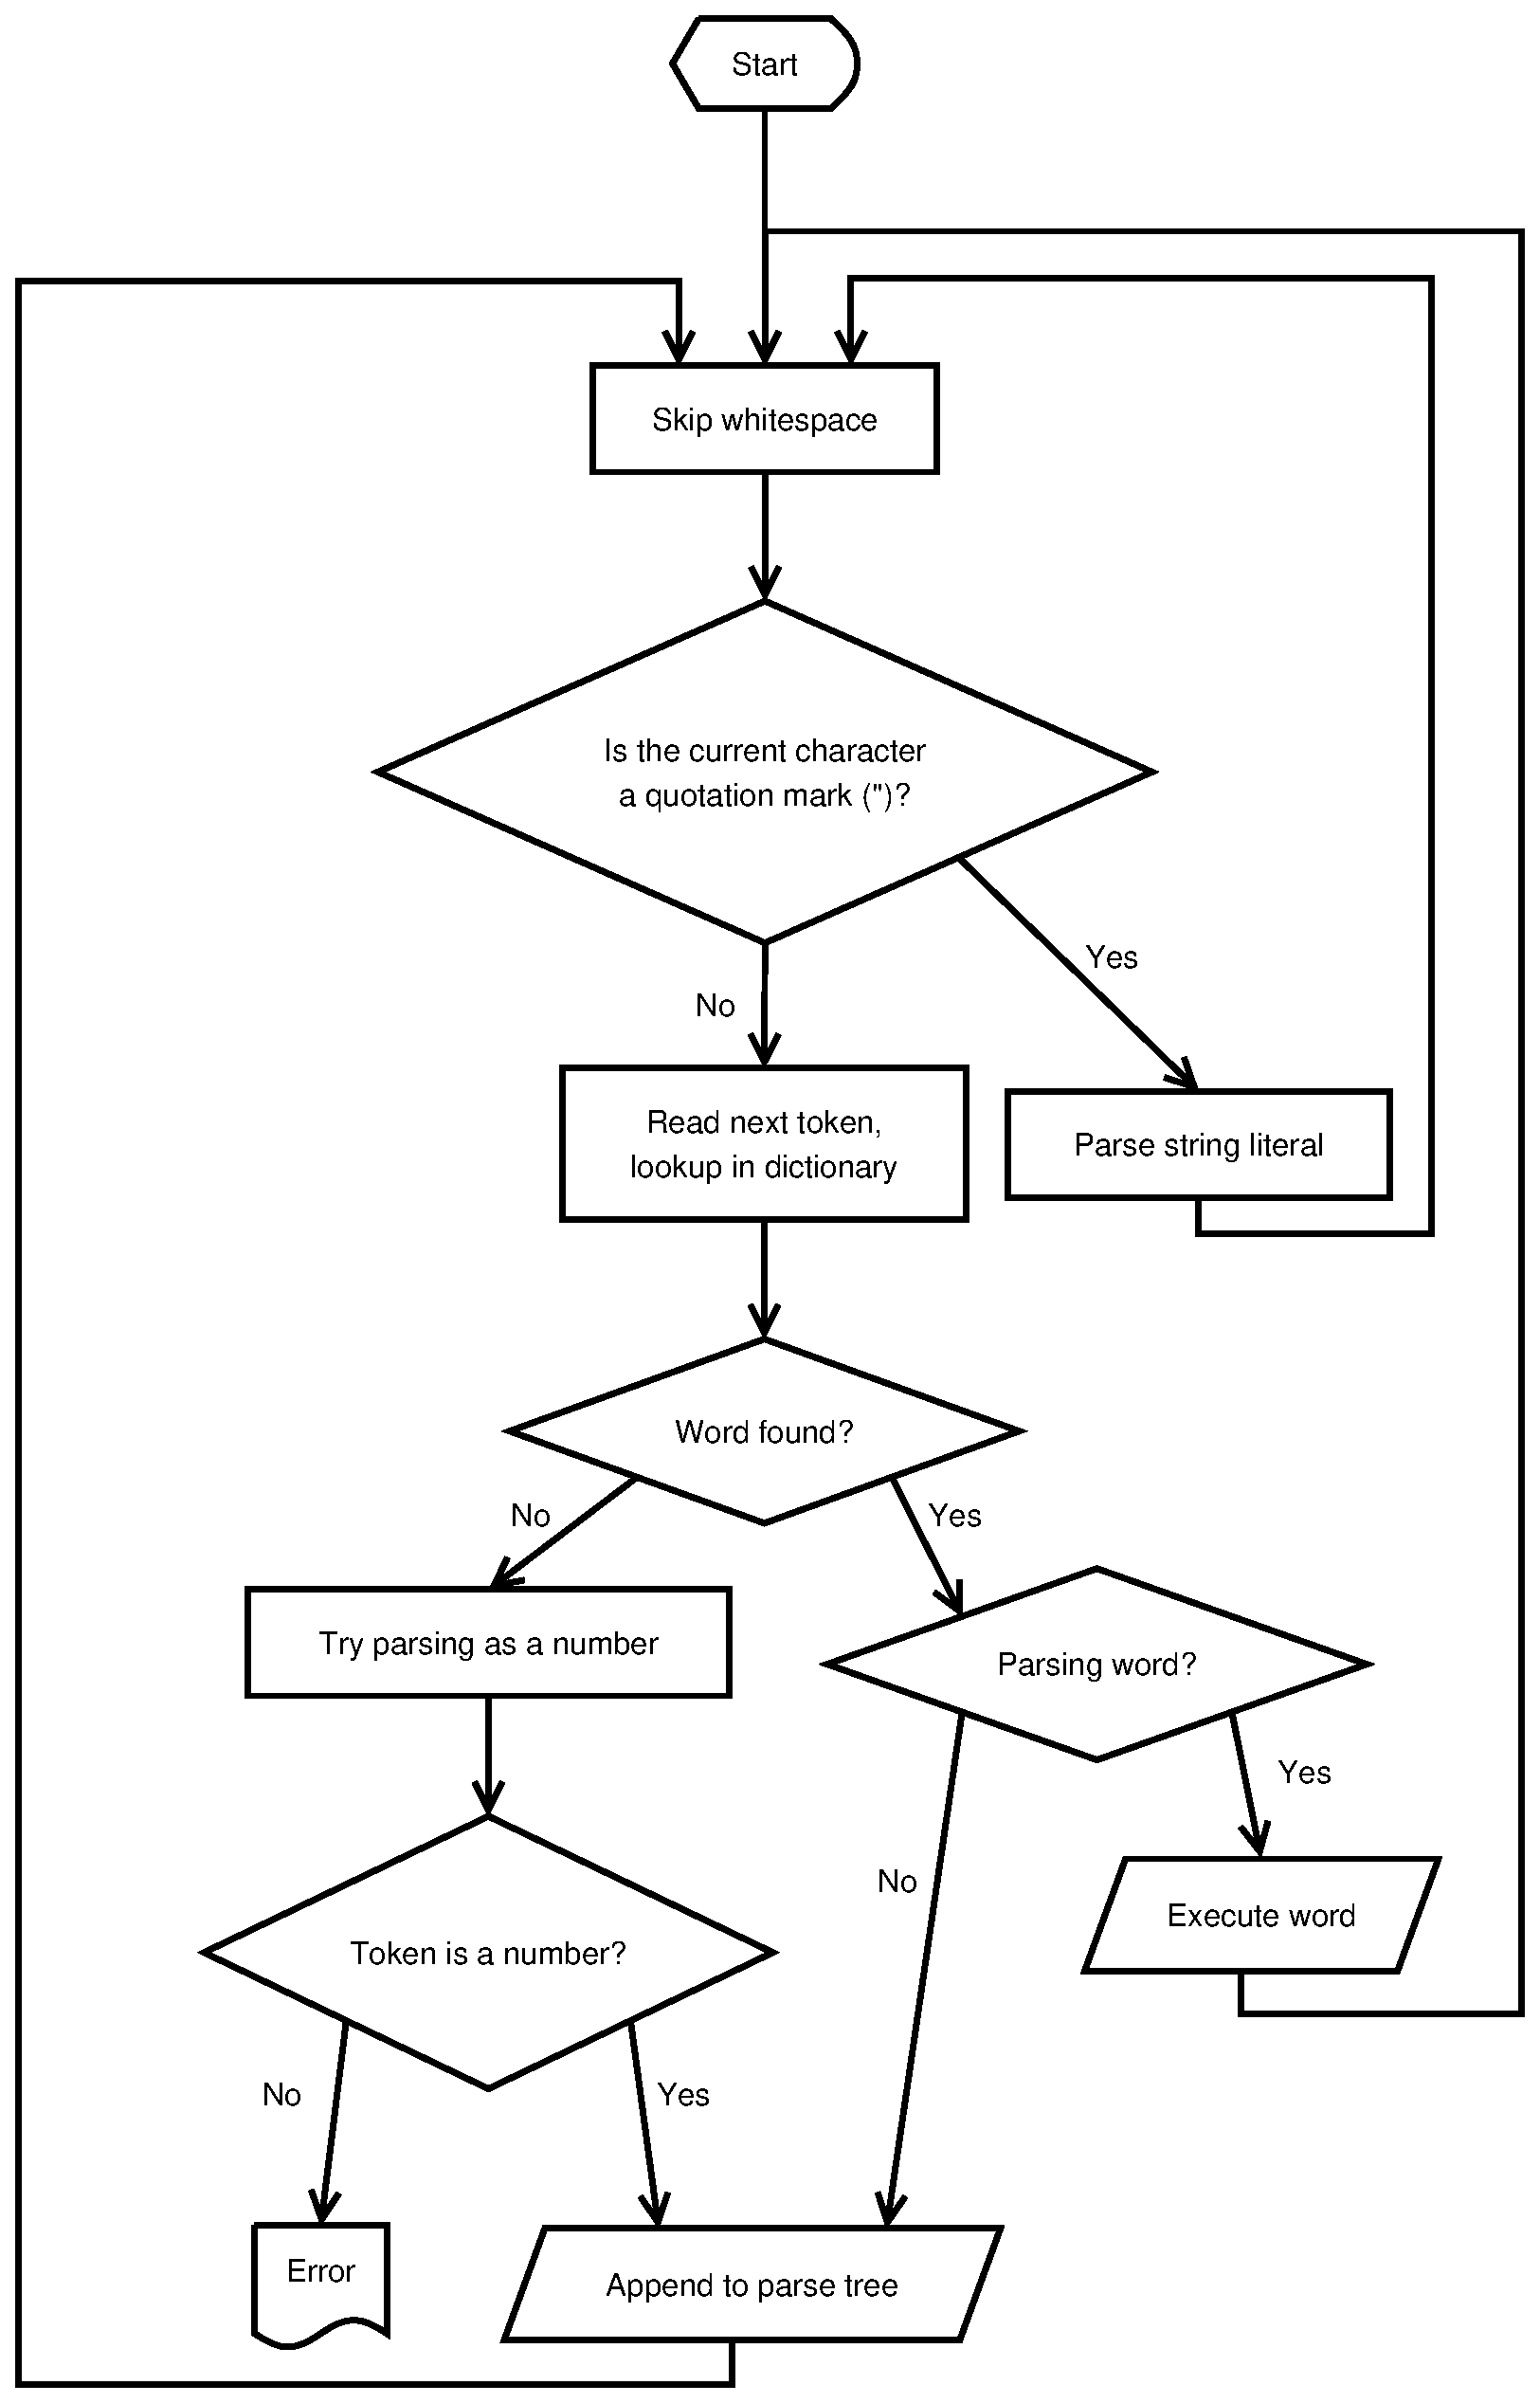
\epsfig{file=parser.eps}}
\end{center}
\end{figure}

At the most abstract level,
Factor syntax consists of whitespace-separated tokens. The parser tokenizes the input on whitespace boundaries, where whitespace is defined as a sequence or one or more space, tab, newline or carriage-return characters.  The parser is case-sensitive, so
the following three expressions tokenize differently:
\begin{verbatim}
2X+
2 X +
2 x +
\end{verbatim}
As the parser reads tokens it makes a distinction between numbers, ordinary words, and
parsing words. Tokens are appended to the parse tree, the top level of which is a list
returned by the original parser invocation. Nested levels of the parse tree are created
by parsing words.

Here is the parser algorithm in more detail -- some of the concepts therein will be defined shortly:

\begin{itemize}
\item If the current character is a double-quote (\texttt{"}), the \texttt{"} parsing word is executed, causing a string to be read.
\item Otherwise, the next token is taken from the input. The parser searches for a word named by the token in the currently used set of vocabularies. If the word is found, one of the following two actions is taken:
\begin{itemize}
\item If the word is an ordinary word, it is appended to the parse tree.
\item If the word is a parsing word, it is executed.
\end{itemize}
Otherwise if the token does not represent a known word, the parser attempts to parse it as a number. If the token is a number, the number object is added to the parse tree. Otherwise, an error is raised and parsing halts.
\end{itemize}

\glossary{name=string mode,
description={a parser mode where token strings are added to the parse tree; the parser will not look up tokens in the dictionary. Activated by switching on the \texttt{string-mode} variable}}

There is one exception to the above process; the parser might be placed in \emph{string mode}, in which case it simply reads tokens and appends them to the parse tree as strings. String mode is activated and deactivated by certain parsing words wishing to read input in an unstructured but tokenized manner -- see \ref{string-mode}.

\glossary{name=parsing word,
description={a word that is run at parse time. Parsing words can be defined by suffixing the compound definition with \texttt{parsing}. Parsing words have the \texttt{\dq{}parsing\dq{}} word property set to true, and respond with true to the \texttt{parsing?}~word}}

Parsing words play a key role in parsing; while ordinary words and numbers are simply
added to the parse tree, parsing words execute in the context of the parser, and can
do their own parsing and create nested data structures in the parse tree. Parsing words
are also able to define new words.

While parsing words supporting arbitrary syntax can be defined, the default set is found
in the \texttt{syntax} vocabulary and provides the basis for all further syntactic
interaction with Factor.

\subsection{\label{vocabsearch}Vocabulary search}

\newcommand{\wordglos}{\glossary{
name=word,
description={an object holding a code definition and set of properties. Words are organized into vocabularies, and are uniquely identified by name within a vocabulary.}}}
\wordglos
\newcommand{\vocabglos}{\glossary{
name=vocabulary,
description={a collection of words, uniquely identified by name. The hashtable of vocabularies is stored in the \texttt{vocabularies} global variable, and the \texttt{USE:}~and \texttt{USING:}~parsing words add vocabularies to the parser's search path}}}
\vocabglos

A \emph{word} associates a code definition with its name. Words are organized into \emph{vocabularies}. Vocabularies are organized into vocabularies. Words are discussed in depth in \ref{words}.

When the parser reads a token, it attempts to look up a word named by that token. The
lookup is performed in the parser's current vocabulary set. By default, this set includes
two vocabularies:
\begin{verbatim}
syntax
scratchpad
\end{verbatim}
The \texttt{syntax} vocabulary consists of a set of parsing words for reading Factor data
and defining new words. The \texttt{scratchpad} vocabulary is the default vocabulary for new
word definitions.
\wordtable{
\parsingword{USE:}{USE: \emph{vocabulary}}{syntax}
}
\newcommand{\useglos}{\glossary{
name=search path,
description={the list of vocabularies that the parser looks up tokens in. You can add to this list with the \texttt{USE:} and \texttt{USING:} parsing words}}}
\useglos

The \texttt{USE:} parsing word adds a new vocabulary at the front of the search path. Subsequent word lookups by the parser will search this vocabulary first.
\begin{alltt}
USE: lists
\end{alltt}
\wordtable{
\parsingword{USING:}{USING: \emph{vocabularies} ;}{syntax}
}
Consecutive \texttt{USE:} declarations can be merged into a single \texttt{USING:} declaration.
\begin{alltt}
USING: lists strings vectors ;
\end{alltt}

Due to the way the parser works, words cannot be referenced before they are defined; that is, source files must order definitions in a strictly bottom-up fashion. For a way around this, see \ref{deferred}.

\subsection{Numbers}

\newcommand{\numberglos}{\glossary{
name=number,
description={an instance of the \texttt{number} class}}}
\numberglos

If a vocabulary lookup of a token fails, the parser attempts to parse it as a number.

\subsubsection{Integers}

\newcommand{\integerglos}{\glossary{
name=integer,
description={an instance of the \texttt{integer} class, which is a disjoint union of the \texttt{fixnum} and \texttt{bignum} classes}}}
\numberglos

\newcommand{\fixnumglos}{\glossary{
name=fixnum,
description={an instance of the \texttt{fixnum} class, representing a fixed precision integer. On 32-bit systems, an element of the interval $(-2^{-29},2^{29}]$, and on 64-bit systems, the interval $(-2^{-61},2^{61}]$}}}
\fixnumglos

\newcommand{\bignumglos}{\glossary{
name=bignum,
description={an instance of the \texttt{bignum} class, representing an arbitrary-precision integer whose value is bounded by available object memory}}}
\bignumglos

The printed representation of an integer consists of a sequence of digits, optionally prefixed by a sign.
\begin{alltt}
123456
-10
2432902008176640000
\end{alltt}
Integers are entered in base 10 unless prefixed with a base change parsing word.
\wordtable{
\parsingword{BIN:}{BIN: \emph{integer}}{syntax}\\
\parsingword{OCT:}{OCT: \emph{integer}}{syntax}\\
\parsingword{HEX:}{HEX: \emph{integer}}{syntax}
}
\begin{alltt}
\textbf{ok} BIN: 1110 BIN: 1 + .
\textbf{15}
\textbf{ok} HEX: deadbeef 2 * .
\textbf{7471857118}
\end{alltt}

\subsubsection{Ratios}

\newcommand{\ratioglos}{\glossary{
name=ratio,
description={an instance of the \texttt{ratio} class, representing an exact ratio of two integers}}}
\ratioglos

The printed representation of a ratio is a pair of integers separated by a slash (\texttt{/}).
No intermediate whitespace is permitted. Either integer may be signed, however the ratio will be normalized into a form where the denominator is positive and the greatest common divisor
of the two terms is 1.
\begin{alltt}
75/33
1/10
-5/-6
\end{alltt}

\subsubsection{Floats}

\newcommand{\floatglos}{\glossary{
name=float,
description={an instance of the \texttt{float} class, representing an IEEE 754 double-precision floating point number}}}
\floatglos

Floating point numbers contain an optional decimal part, an optional exponent, with
an optional sign prefix on either the significand or exponent.
\begin{alltt}
10.5
-3.1456
7e13
1e-5
\end{alltt}

\subsubsection{Complex numbers}

\newcommand{\complexglos}{\glossary{
name=complex,
description={an instance of the \texttt{complex} class, representing a complex number with real and imaginary components, where both components are real numbers}}}
\complexglos
\wordtable{
\parsingword{hash-curly}{\#\{ \emph{real} \emph{imaginary} \}\#}{syntax}
}
A complex number
is given by two components, a ``real'' part and ''imaginary'' part. The components
must either be integers, ratios or floats.
\begin{verbatim}
#{ 1/2 1/3 }#   ! the complex number 1/2+1/3i
#{ 0 1 }#       ! the imaginary unit
\end{verbatim}

\subsection{Literals}

Many different types of objects can be constructed at parse time via literal syntax. Numbers are a special case since support for reading them is built-in to the parser. All other literals are constructed via parsing words.

If a quotation contains a literal object, the same literal object instance is used each time the quotation executes; that is, literals are ``live''.

\subsubsection{\label{boolean}Booleans}

\newcommand{\boolglos}{
\glossary{
name=boolean,
description={an instance of the \texttt{boolean} class, either \texttt{f} or \texttt{t}. See generalized boolean}}
\glossary{
name=generalized boolean,
description={an object used as a truth value. The \texttt{f} object is false and anything else is true. See boolean}}
\glossary{
name=t,
description={the canonical truth value. The \texttt{t} class, whose sole instance is the \texttt{t} object. Note that the \texttt{t} class is not equal to the \texttt{t} object}}
\glossary{
name=f,
description={the canonical false value; anything else is true. The \texttt{f} class, whose sole instance is the \texttt{f} object. Note that the \texttt{f} class is not equal to the \texttt{f} object}}
}
\boolglos
Any Factor object may be used as a truth value in a conditional expression. The \texttt{f} object is false and anything else is true. The \texttt{f} object is also used to represent the empty list, as well as the concept of a missing value. The canonical truth value is the \texttt{t} object.
\wordtable{
\parsingword{f}{f}{syntax}\\
\parsingword{t}{t}{syntax}
}
Adds the \texttt{f} and \texttt{t} objects to the parse tree.

Note that the \texttt{f} parsing word and class is not the same as the \texttt{f} object. The former can be obtained by writing \texttt{\bs~f} inside a quotation, or \texttt{POSTPONE: f} inside a list that will not be evaluated.
\begin{alltt}
\textbf{ok} f \bs f = .
\textbf{f}
\end{alltt}
An analogous distinction holds for the \texttt{t} class and object.

\subsubsection{\label{syntax:char}Characters}

\newcommand{\charglos}{\glossary{
name=character,
description={an integer whose value denotes a Unicode code point. Character values are limited to the range from $0$ to $2^16-1$ inclusive, however in a later release this can be upgraded to the full 21-bit Unicode space without requiring any changes to user code}}}
\charglos
Factor has no distinct character type, however Unicode character value integers can be
read by specifying a literal character, or an escaped representation thereof.
\wordtable{
\parsingword{CHAR:}{CHAR: \emph{token}}{syntax}
}
Adds the Unicode code point of the character represented by \emph{token} to the parse tree.

\newcommand{\escapeglos}{\glossary{
name=escape,
description={a sequence allowing a non-literal character to be inserted in a string. For a list of escapes, see \ref{escape}}}}
\escapeglos
If the token is a single-character string other than whitespace or backslash, the character is taken to be this token. If the token begins with a backslash, it denotes one of the following escape codes.
\begin{table}[Special character escape codes]
\label{escape}
\begin{tabular}{l|l}
Escape code&Character\\
\hline
\texttt{\bs{}\bs}&Backslash (\texttt{\bs})\\
\texttt{\bs{}s}&Space\\
\texttt{\bs{}t}&Tab\\
\texttt{\bs{}n}&Newline\\
\texttt{\bs{}t}&Carriage return\\
\texttt{\bs{}0}&Null byte (ASCII 0)\\
\texttt{\bs{}e}&Escape (ASCII 27)\\
\texttt{\bs{}"}&Double quote (\texttt{"})\\
\end{tabular}
\end{table}
Examples:
\begin{alltt}
\textbf{ok} CHAR: a .
\textbf{97}
\textbf{ok} CHAR: \bs{}0 .
\textbf{0}
\textbf{ok} CHAR: \bs{}n .
\textbf{10}
\end{alltt}
A Unicode character can be specified by its code number by writing \texttt{\bs{}u} followed by a four-digit hexadecimal. That is, the following two expressions are equivalent:
\begin{alltt}
CHAR: \bs{}u0078
78
\end{alltt}
While not useful for single characters, this syntax is also permitted inside strings.

\subsubsection{\label{string-literals}Strings}

\newcommand{\stringglos}{\glossary{
name=string,
description={an instance of the \texttt{string} class, representing an immutable sequence of characters}}}
\stringglos
\wordtable{
\parsingword{"}{"\emph{string}"}{syntax}
}
Reads from the input string until the next occurrence of
\texttt{"}, and appends the resulting string to the parse tree. String literals cannot span multiple lines.
Strings containing
the \texttt{"} character and various other special characters can be read by
inserting escape sequences as described in \ref{syntax:char}.
\begin{alltt}
\textbf{ok} "Hello world" print
\textbf{Hello world}
\end{alltt}

\subsubsection{\label{listsyntax}Lists}
\newcommand{\listglos}{\glossary{
name=list,
description={an instance of the \texttt{list} class, storing a sequence of elements as a chain of zero or more conses, where the car of each cons is an element, and the cdr is either \texttt{f} or another list}}
\glossary{name=proper list, description=see list}
}
\listglos
\wordtable{
\parsingword{openbracket}{[}{syntax}\\
\parsingword{closebracket}{]}{syntax}
}
Parses a list, whose elements are read between \texttt{[} and \texttt{]} and can include other lists.
\begin{verbatim}
[
    "404" "responder" set
    [ drop no-such-responder ] "get" set
]
\end{verbatim}
\newcommand{\consglos}{\glossary{
name=cons,
description={an instance of the \texttt{cons} class, storing an ordered pair of objects referred to as the car and the cdr}}}
\consglos
\wordtable{
\parsingword{conssyntax}{[[ \emph{car} \emph{cdr} ]]}{syntax}
}
Parses two components making up a cons cell. Note that the lists parsed with \texttt{[} and \texttt{]} are just a special case of \texttt{[[} and \texttt{]]}. The following two lines are equivalent.
\begin{alltt}
[ 1 2 3 ]
[[ 1 [[ 2 [[ 3 f ]] ]] ]]
\end{alltt}
The empty list is denoted by \texttt{f}, along with boolean falsity, and the concept of a missing value. The expression \texttt{[ ]} parses to the same object as \texttt{f}.

\subsubsection{Words}

While words parse as themselves, a word occurring inside a quotation is executed when the quotation is called. Sometimes it is desirable to have a word be pushed on the data stack during the execution of a quotation, usually for reflective access to the word's slots.
\wordtable{
\parsingword{bs}{\bs~\emph{word}}{syntax}
}
Reads the next word from the input string and appends some \emph{code} to the parse tree that pushes the word on the stack when the code is called. The following two lines are equivalent:
\begin{verbatim}
\ length
[ length ] car
\end{verbatim}
\wordtable{
\parsingword{POSTPONE:}{POSTPONE: \emph{word}}{syntax}
}
Reads the next word from the input string and appends the word to the parse tree, even if it is a parsing word. For an word \texttt{foo}, \texttt{POSTPONE: foo} and \texttt{foo} are equivalent; however, if \texttt{foo} is a parsing word, the latter will execute it at parse time, while the former will execute it at runtime. Usually used inside parsing words that wish to delegate some action to a further parsing word.
\begin{alltt}
\textbf{ok} : parsing1
    "Parsing 1" print 2 swons ; parsing
\textbf{ok} : parsing2
    "Parsing 2" print POSTPONE: parsing1 ; parsing
\textbf{ok} [ 1 parsing1 3 ] .
\textbf{Parsing 1}
\textbf{[ 1 2 3 ]}
\textbf{ok} [ 0 parsing2 2 4 ] .
\textbf{Parsing 2}
\textbf{Parsing 1}
\textbf{[ 0 2 4 ]}
\end{alltt}

\subsubsection{Mutable literals}

\newcommand{\mutableglos}{\glossary{name=mutable object,
description=an object whose slot values can be changed}
\glossary{name=immutable object,
description=an object whose slot values cannot be changed}}
\mutableglos

Using mutable object literals in word definitions requires care, since if those objects
are mutated, the actual word definition will be changed, which is in most cases not what you would expect. Strings and lists are immutable; string buffers, vectors, hashtables and tuples are mutable.

\subsubsection{\label{sbuf-literals}String buffers}

\newcommand{\sbufglos}{\glossary{
name=string buffer,
description={an instance of the \texttt{sbuf} class, representing a mutable and growable sequence of characters}}
\glossary{name=sbuf, description=see string buffer}}
\sbufglos
\wordtable{
\parsingword{SBUF}{SBUF" \emph{text}"}{syntax}
}
Reads from the input string until the next occurrence of
\texttt{"}, converts the string to a string buffer, and appends it to the parse tree.
As with strings, the escape codes described in \ref{syntax:char} are permitted.
\begin{alltt}
\textbf{ok} SBUF" Hello world" sbuf>string print
\textbf{Hello world}
\end{alltt}

\subsubsection{\label{vector-literals}Vectors}
\newcommand{\vectorglos}{\glossary{
name=vector,
description={an instance of the \texttt{vector} class, storing a mutable and growable sequence of elements in a contiguous range of memory}}}
\vectorglos
\wordtable{
\parsingword{opencurly}{\{}{syntax}\\
\parsingword{closecurly}{\}}{syntax}
}
Parses a vector, whose elements are read between \texttt{\{} and \texttt{\}}.
\begin{verbatim}
{ 3 "blind" "mice" }
\end{verbatim}

\subsubsection{Hashtables}
\newcommand{\hashglos}{\glossary{
name=hashtable,
description={an instance of the \texttt{hashtable} class, providing a mutable mapping of keys to values}}}
\hashglos
\wordtable{
\parsingword{openccurly}{\{\{}{syntax}\\
\parsingword{closeccurly}{\}\}}{syntax}
}
Parses a hashtable. Elements between \texttt{\{\{} and \texttt{\}\}} must be cons cells, where the car is the key and the cdr is a value.
\begin{verbatim}
{{
    [[ "red" [ 255 0 0 ] ]]
    [[ "green" [ 0 255 0 ] ]]
    [[ "blue" [ 0 0 255 ] ]]
}}
\end{verbatim}

\subsubsection{Tuples}
\newcommand{\tupleglos}{\glossary{
name=tuple,
description={an instance of a user-defined class whose metaclass is the \texttt{tuple} metaclass, storing a fixed set of elements in named slots, with optional delegation method dispatch semantics}}}
\tupleglos
\wordtable{
\parsingword{<<}{<<}{syntax}\\
\parsingword{>>}{>>}{syntax}
}
Parses a tuple. The tuple's class must follow \texttt{<<}. The element after that is always the tuple's delegate. Further elements until \texttt{>>} are specified according to the tuple's slot definition, and an error is raised if an incorrect number of elements is given.
\begin{verbatim}
<< color f 255 0 0 >>
\end{verbatim}

\subsection{\label{comments}Comments}

\wordtable{
\parsingword{!}{!~\emph{remainder of line}}{syntax}
}
The remainder of the input line is ignored if an exclamation mark (\texttt{!}) is read.
\begin{alltt}
! Note that the sequence union does not include lists,
! or user defined tuples that respond to the sequence
! protocol.
\end{alltt}
\wordtable{
\parsingword{hash!}{\#!~\emph{remainder of line}}{syntax}
}
\newcommand{\doccommentglos}{\glossary{
name=documentation comment,
description={a comment describing the usage of a word. Delimited by the \texttt{\#"!} parsing word, they appear at the start of a word definition and are stored in the \texttt{""documentation""} word property}}}
\doccommentglos
Comments that begin with \texttt{\#!} are called \emph{documentation comments}.
A documentation comment has no effect on the generated parse tree, but if it is the first thing inside a word definition, the comment text is appended to the string stored in the word's \texttt{"documentation"} property. Word properties are described in \ref{word-props}.
\wordtable{
\parsingword{(}{( \emph{stack effect} )}{syntax}
}
\glossary{
name=stack effect,
description={A string of the form \texttt{( \emph{inputs} -- \emph{outputs} )}, where the inputs and outputs are a whitespace-separated list of names or types. The top of the stack is the right-most token on both sides.}}
\newcommand{\stackcommentglos}{\glossary{
name=stack effect comment,
description={a comment describing the inputs and outputs of a word. Delimited by \texttt{(} and \texttt{}), they appear at the start of a word definition and are stored in the \texttt{""stack-effect""} word property}}}
\stackcommentglos
Comments delimited by \texttt{(} and \texttt{)} are called \emph{stack effect comments}. By convention they are placed at the beginning of a word definition to document the word's inputs and outputs:
\begin{verbatim}
: push ( element sequence -- )
    #! Push a value on the end of a sequence.
    dup length swap set-nth ;
\end{verbatim}
A stack effect comment has no effect on the generated parse tree, but if it is the first thing inside a word definition, the word's \texttt{"stack-effect"} property is set to the comment text. Word properties are described in \ref{word-props}.

\section{Data and control flow}

\subsection{Shuffle words}

\newcommand{\dsglos}{\glossary{
name=stack,
description=see data stack}
\glossary{
name=data stack,
description={the primary means of passing values between words}}}
\dsglos
Shuffle words are placed between words taking action to rearrange items on the stack
as the next word in the quotation would expect them. Their behavior can be understood entirely in terms of their stack effects.
\wordtable{
\ordinaryword{drop}{drop ( x -- )}{kernel}\\
\ordinaryword{2drop}{drop ( x y -- )}{kernel}\\
\ordinaryword{3drop}{drop ( x y z -- )}{kernel}\\
\ordinaryword{nip}{nip ( x y -- y )}{kernel}\\
\ordinaryword{2nip}{2nip ( x y -- y )}{kernel}\\
\ordinaryword{dup}{dup ( x -- x x )}{kernel}\\
\ordinaryword{2dup}{2dup ( x y -- x y x y )}{kernel}\\
\ordinaryword{3dup}{3dup ( x y z -- x y z x y z )}{kernel}\\
\ordinaryword{dupd}{dupd ( x y -- x x y )}{kernel}\\
\ordinaryword{over}{over ( x y -- x y x )}{kernel}\\
\ordinaryword{pick}{pick ( x y z -- x y z x )}{kernel}\\
\ordinaryword{tuck}{tuck ( x y -- y x y )}{kernel}\\
\ordinaryword{swap}{swap ( x y -- y x )}{kernel}\\
\ordinaryword{2swap}{2swap ( x y z t -- z t x y )}{kernel}\\
\ordinaryword{swapd}{swapd ( x y z -- y x z )}{kernel}\\
\ordinaryword{rot}{rot ( x y z -- y z x )}{kernel}\\
\ordinaryword{-rot}{-rot ( x y z -- z x y )}{kernel}
}
Try to avoid the complex shuffle words such as \texttt{rot} and \texttt{2dup} as much as possible, for they make data flow harder to understand. If you find yourself using too many shuffle words, or you're writing
a stack effect comment in the middle of a compound definition to keep track of stack contents, it is
a good sign that the word should probably be factored into two or
more smaller words.

\subsection{\label{quotations}Quotations}

\newcommand{\csglos}{\glossary{
name=return stack,
description=see call stack}
\glossary{
name=call stack,
description={holds quotations waiting to be called. When a quotation is called with \texttt{call}, or when a compound word is executed, the previous call frame is pushed on the call stack, and the new quotation becomes the current call frame}}}
\csglos
\newcommand{\cfglos}{\glossary{
name=call frame,
description=the currently executing quotation}}
\cfglos
\glossary{
name=interpreter,
description=executes quotations by iterating them and recursing into nested definitions. see compiler}

\begin{figure}
\begin{center}
\caption{Interpreter algorithm}
\scalebox{0.45}{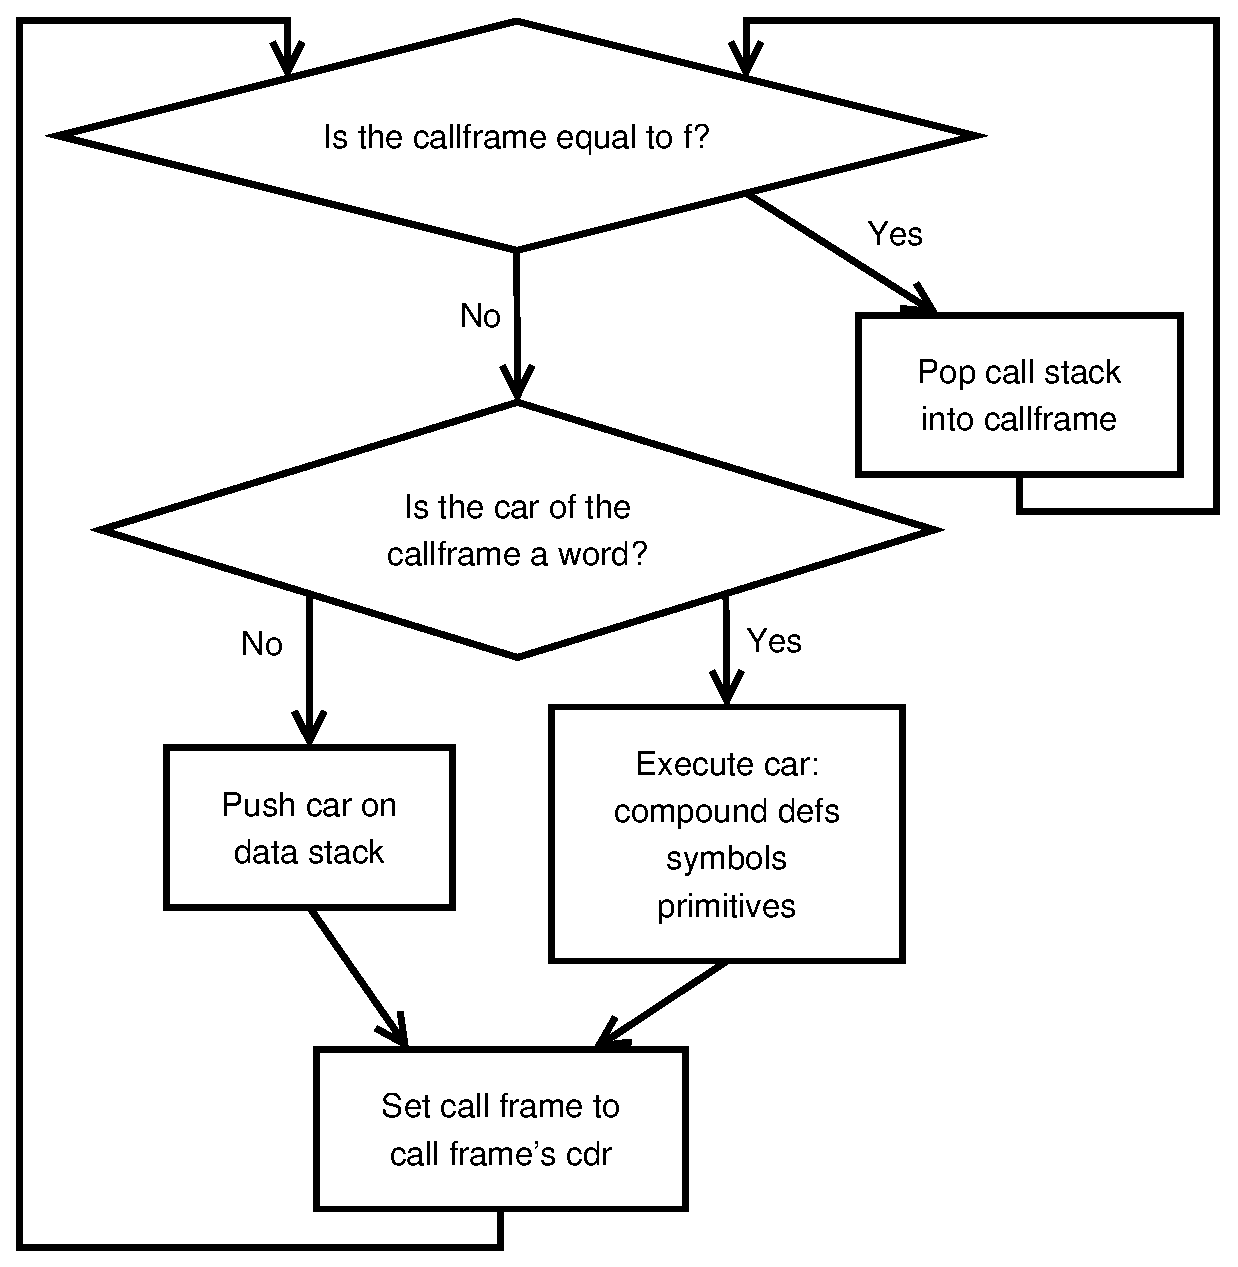
\epsfig{file=interpreter.eps}}
\end{center}
\end{figure}

The Factor interpreter executes quotations. Quotations are lists, and since lists can contain any Factor object, they can contain words. It is words that give quotations their operational behavior, as you can see in the following description of the interpreter algorithm.

\begin{itemize}
\item If the call frame is \texttt{f}, the call stack is popped and becomes the new call frame.
\item If the car of the call frame is a word, the word is executed:
\begin{itemize}
\item If the word is a symbol, it is pushed on the data stack. See \ref{symbols}.
\item If the word is a compound definition, the current call frame is pushed on the call stack, and the new call frame becomes the word definition. See \ref{colondefs}.
\item If the word is compiled or primitive, the interpreter jumps to a machine code definition. See \ref{primitives}.
\item If the word is undefined, an error is raised. See \ref{deferred}.
\end{itemize}
\item Otherwise, the car of the call frame is pushed on the data stack.
\item The call frame is set to the cdr, and the loop continues.
\end{itemize}

The interpreter can be invoked reflectively with the following pair of words.
\wordtable{
\ordinaryword{call}{call ( quot -- )}{kernel}
}
Push the current call frame on the call stack, and set the call stack to the given quotation. Conceptually: calls the quotation, as if its definition was substituted at the location of the \texttt{call}.
\begin{alltt}
\textbf{ok} [ 2 2 + 3 * ] call .
\textbf{12}
\end{alltt}
\wordtable{
\ordinaryword{execute}{execute ( word -- )}{kernel}
}
Execute a word definition, taking action based on the word definition, as above.
\begin{alltt}
\textbf{ok} : hello "Hello world" print ;
\textbf{ok} : twice dup execute execute ;
\textbf{ok} \bs hello twice
\textbf{Hello world}
\textbf{Hello world}
\end{alltt}

\subsubsection{Tail call optimization}

\newcommand{\tailglos}{\glossary{
name=tail call,
description=the last call in a quotation}
\glossary{
name=tail call optimization,
description=the elimination of call stack pushes when making a tail call}}

When a call is made to a quotation from the last word in the call frame, there is no
purpose in pushing the empty call frame on the call stack. Therefore the last call in a quotation does not grow the call stack, and tail recursion executes in bounded space.

\subsubsection{Call stack manipulation}

Because of the way the interpreter is described in \ref{quotations}, the top of the call stack is not accessed during the execution of a quotation; it is only popped when the interpreter reaches the end of the quotation. In effect, the call stack can be used as a temporary storage area, as long as pushes and pops are balanced out within a single quotation.
\wordtable{
\ordinaryword{>r}{>r ( x -- r:x )}{kernel}
}
Moves the top of the data stack to the call stack.
\wordtable{
\ordinaryword{r>}{r> ( x -- r:x )}{kernel}
}
Moves the top of the call stack to the data stack.

The top of the data stack is ``hidden'' between \texttt{>r} and \texttt{r>}.
\begin{alltt}
\textbf{ok} 1 2 3 >r .s r>
\textbf{2
1}
\end{alltt}
It is very important to balance usages of \texttt{>r} and \texttt{r>} within a single quotation or word definition.
\begin{verbatim}
: the-good >r 2 + r> * ; ! Okay
: the-bad  >r 2 + ;      ! Runtime error
: the-ugly r> ;          ! Runtime error
\end{verbatim}
Basically, the rule is you must leave the call stack in the same state as you found it, so that when the current quotation finishes executing, the interpreter can return to the caller.

One exception is that when \texttt{ifte} occurs as the last word in a definition, values may be pushed on the call stack before the condition value is computed, as long as both branches of the \texttt{ifte} pop the values off the call stack before returning.
\begin{verbatim}
: foo ( m ? n -- m+n/n )
    >r [ r> + ] [ drop r> ] ifte ; ! Okay
\end{verbatim}

\subsubsection{Quotation variants}

There are three words that combine shuffle words with \texttt{call}. They are useful in the implementation of higher-order words taking quotations as inputs.
\wordtable{
\ordinaryword{slip}{slip ( quot x -- x | quot: -- )}{kernel}
}
Call a quotation, while hiding the top of the stack. The implementation is as you would expect.
\begin{verbatim}
: slip ( quot x -- x | quot: -- )
    >r call r> ; inline
\end{verbatim}
\wordtable{
\ordinaryword{keep}{keep ( x quot -- x | quot:~x -- )}{kernel}
}
Call a quotation with a value on the stack, restoring the value when the quotation returns.
\begin{verbatim}
: keep ( x quot -- x | quot: x -- )
    over >r call r> ; inline
\end{verbatim}
\wordtable{
\ordinaryword{2keep}{2keep ( x y q -- x y | q:~x y -- )}{kernel}
}
Call a quotation with a pair of values on the stack, restoring the values when the quotation returns.
\begin{verbatim}
: 2keep ( x y quot -- x y | quot: x y -- )
    over >r pick >r call r> r> ; inline
\end{verbatim}

\subsection{Conditionals}

The simplest style of a conditional form is the \texttt{ifte} word.
\wordtable{
\ordinaryword{ifte}{ifte ( cond true false -- )}{kernel}
}
The \texttt{cond} is a generalized boolean. If it is \texttt{f}, the \texttt{false} quotation is called, and if \texttt{cond} is any other value, the \texttt{true} quotation is called. The condition flag is removed from the stack before either quotation executes.

Note that in general, both branches should have the same stack effect. Not only is this good style that makes the word easier to understand, but also unbalanced conditionals cannot be compiled.
\wordtable{
\ordinaryword{when}{when ( cond true -- | true:~-- )}{kernel}\\
\ordinaryword{unless}{unless ( cond false -- | false:~-- )}{kernel}
}
This pair are minor variations on \texttt{ifte} where only one branch is specified. The other is implicitly \texttt{[ ]}. They are implemented in the trivial way:
\begin{verbatim}
: when [ ] ifte ; inline
: unless [ ] swap ifte ; inline
\end{verbatim}
The \texttt{ifte} word removes the condition flag from the stack before calling either quotation. Sometimes this is not desirable, if the condition flag is serving a dual purpose as a value to be consumed by the \texttt{true} quotation. The \texttt{ifte*} word exists for this purpose.
\wordtable{
\ordinaryword{ifte*}{ifte*~( cond true false -- )}{kernel}\\
\texttt{true:~cond --}\\
\texttt{false:~--}
}
If the condition is true, it is retained on the stack before the \texttt{true} quotation is called. Otherwise, the condition is removed from the stack and the \texttt{false} quotation is called. The following two lines are equivalent:
\begin{verbatim}
X [ Y ] [ Z ] ifte*
X dup [ Y ] [ drop Z ] ifte
\end{verbatim}
\wordtable{
\ordinaryword{when*}{when*~( cond true -- | true:~cond -- )}{kernel}\\
\ordinaryword{unless*}{unless*~( cond false -- | false:~-- )}{kernel}
}
These are variations of \texttt{ifte*} where one of the quotations is \texttt{[ ]}.

There is one final conditional form that is used to implement the ``default value'' idiom.
\wordtable{
\ordinaryword{?ifte}{?ifte ( default cond true false -- )}{kernel}\\
\texttt{true:~cond --}\\
\texttt{false:~default --}
}
If the condition is \texttt{f}, the \texttt{false} quotation is called with the \texttt{default} value on the stack. Otherwise, the \texttt{true} quotation is called with the condition on the stack. The following two lines are equivalent:
\begin{verbatim}
X [ Y ] [ Z ] ?ifte
X dup [ nip Y ] [ drop Z ] ifte
\end{verbatim}

\subsubsection{Boolean logic}

The \texttt{?}~word chooses between two values, rather than two quotations.
\wordtable{
\ordinaryword{?}{?~( cond true false -- true/false )}{kernel}
}
It is implemented in the obvious way.
\begin{verbatim}
: ? ( cond t f -- t/f )
    rot [ drop ] [ nip ] ifte ; inline
\end{verbatim}
Several words use \texttt{?}~to implement typical boolean algebraic operations.
\wordtable{
\ordinaryword{>boolean}{>boolean ( obj -- t/f )}{kernel}
}
Convert a generalized boolean into a boolean. That is, \texttt{f} retains its value, whereas anything else becomes \texttt{t}.
\wordtable{
\ordinaryword{not}{not ( ?~-- ?~)}{kernel}
}
Given \texttt{f}, outputs \texttt{t}, and on any other input, outputs \texttt{f}.
\wordtable{
\ordinaryword{and}{and ( ?~?~-- ?~)}{kernel}
}
Outputs \texttt{t} if both of the inputs are true.
\wordtable{
\ordinaryword{or}{or ( ?~?~-- ?~)}{kernel}
}
Outputs \texttt{t} if at least one of the inputs is true.
\wordtable{
\ordinaryword{xor}{xor ( ?~?~-- ?~)}{kernel}
}
Outputs \texttt{t} if exactly one of the inputs is true.
\wordtable{
\ordinaryword{implies}{implies ( b1~b2~-- ?~)}{kernel}
}
Outputs \texttt{t} if \texttt{b1} is false or both inputs are true.

An alternative set of logical operations operate on individual bits of integers bitwise, rather than generalized boolean truth values. They are documented in \ref{bitwise}.

\subsection{Continuations}

\newcommand{\contglos}{
\glossary{name=continuation,
description=an object representing the future of the computation}}
\contglos
At any point in the execution of a Factor program, the \emph{current continuation} represents the future of the computation. This object can be captured with the \texttt{callcc0} and \texttt{callcc1} words.
\wordtable{
\ordinaryword{callcc0}{callcc0 ( quot -- )}{kernel}\\
\texttt{quot:~cont --}\\
\texttt{cont:~--}\\
\ordinaryword{callcc1}{callcc1 ( quot -- )}{kernel}\\
\texttt{quot:~cont --}\\
\texttt{cont:~obj --}
}
Calling one of these words calls the given quotation with the continuation on the stack. The continuation is itself a quotation, and calling it \emph{continues execution} at the point after the call to \texttt{callcc0} and \texttt{callcc1}. Essentially, a continuation is a snapshot of the four stacks that can be restored at a later time.

The difference between \texttt{callcc0} and \texttt{callcc1} lies in the continuation object. When \texttt{callcc1} is used, calling the continuation takes one value from the top of the data stack, and places it back on the \emph{restored} data stack. This allows idioms such as exception handling, co-routines and generators to be implemented via continuations.

\subsubsection{\label{exceptions}Handling exceptional situations}
\glossary{name=exception,
description=an object representing an exceptional situation that has been detected}

Support for handling exceptional situations such as bad user input, implementation bugs, and input/output errors is provided by a pair of words, \texttt{throw} and \texttt{catch}.
\wordtable{
\ordinaryword{throw}{throw ( exception -- )}{errors}
}
Raises an exception. Execution does not continue at the point after the \texttt{throw} call. Rather, the innermost catch block is invoked, and execution continues at that point. Passing \texttt{f} as an exception will cause \texttt{throw} to do nothing.
\wordtable{
\ordinaryword{catch}{catch ( try handler -- )}{errors}\\
\texttt{handler:~exception/f -- }
}
An exception handler is established, and the \texttt{try} quotation is called.

If the \texttt{try} quotation throws an error and no nested \texttt{catch} is established, the following sequence of events takes place:
\begin{itemize}
\item the stacks are restored to their state prior to the \texttt{catch} call,
\item the exception is pushed on the data stack,
\item the \texttt{handler} quotation is called.
\end{itemize}
If the \texttt{try} quotation completes successfully, the stacks are \emph{not} restored. The \texttt{f} object is pushed, and the \texttt{handler} quotation is called.

A common idiom is that the \texttt{catch} block cleans up from the error in some fashion, then passes it on to the next-innermost catch block. The following word is used for this purpose.
\wordtable{
\ordinaryword{rethrow}{throw ( exception -- )}{errors}
}
Raises an exception, without saving the current stacks for post-mortem inspection. This is done so that inspecting the error stacks sheds light on the original cause of the exception, rather than the point where it was rethrown.

Here is a simple example of a word definition that attempts to convert a string representing a hexadecimal number into an integer, and instead of halting execution when the string is not valid, it simply outputs \texttt{f}.
\begin{verbatim}
: catch-hex> ( str -- n/f )
    [ hex> ] [ [ drop f ] when ] catch ;
\end{verbatim}
Exception handling is implemented using a \emph{catch stack}. The \texttt{catch} word pushes the current continuation on the catch stack, and \texttt{throw} calls the continuation at the top of the catch stack with the raised exception.
\glossary{name=catch stack,
description={a stack of exception handler continuations, pushed and popped by \texttt{catch}}}

\subsubsection{Multitasking}

Factor implements co-operative multitasking, where the thread of control switches between tasks at explicit calls to \texttt{yield}, as well as when blocking I/O is performed. Multitasking is implemented via continuations.
\wordtable{
\ordinaryword{in-thread}{in-thread ( quot -- )}{threads}
}
Calls \texttt{quot} in a co-operative thread. The new thread begins executing immediately, and the current thread resumes when the quotation yields, either from blocking
I/O or an explicit call to \texttt{yield}. This is implemented by adding the current continuation to the run queue, then calling \texttt{quot}, and finally executing \texttt{stop} after \texttt{quot} returns.
\wordtable{
\ordinaryword{yield}{yield ( -- )}{threads}
}
Add the current continuation to the end of the run queue, and call the continuation at the front of the run queue.
\wordtable{
\ordinaryword{stop}{stop ( -- )}{threads}
}
Call the continuation at the front of run queue, without saving the current continuation. In effect, this stops the current thread.

\subsubsection{Interpreter state}

The current state of the interpreter is determined by the contents of the four stacks. A set of words for getting and setting stack contents are the primitive building blocks for continuations, and in turn abstractions such as exception handling and multitasking.
\wordtable{
\ordinaryword{datastack}{datastack ( -- vector )}{kernel}\\
\ordinaryword{set-datastack}{set-datastack ( vector -- )}{kernel}
}
Save and restore the data stack contents. As an example, here is a word that executes a quotation and restores the data stack to its previous state;
\begin{verbatim}
: keep-datastack
    ( quot -- ) datastack slip set-datastack drop ;
\end{verbatim}
Note that the \texttt{drop} call is made to remove the original quotation from the stack.
\wordtable{
\ordinaryword{callstack}{callstack ( -- vector )}{kernel}\\
\ordinaryword{set-callstack}{set-callstack ( vector -- )}{kernel}
}
Save and restore the call stack contents. The call stack does not include the currently executing quotation that made the call to \texttt{callstack}, since the current quotation is held in the call frame -- \ref{quotations} has details. Similarly, calling \texttt{set-callstack} will continue executing the current quotation until it returns, at which point control transfers to the quotation at the top of the new call stack.
\wordtable{
\ordinaryword{namestack}{namestack ( -- list )}{namespaces}\\
\ordinaryword{set-namestack}{set-namestack ( list -- )}{namespaces}
}
Save and restore the name stack, used for dynamic variable bindings. See \ref{namespaces}.
\wordtable{
\ordinaryword{catchstack}{catchstack ( -- list )}{errors}\\
\ordinaryword{set-catchstack}{set-catchstack ( list -- )}{errors}
}
Save and restore the catch stack, used for exception handling. See \ref{exceptions}.

\section{\label{words}Words}

\wordglos
\vocabglos
\glossary{name=defining word,
description=a word that adds definitions to the dictionary}
\glossary{name=dictionary,
description=the collection of vocabularies making up the code in the Factor image}
Words are the fundamental unit of code in Factor, analogous to functions or procedures in other languages. Words are also objects, and this concept forms the basis for Factor's meta-programming facilities. Words hold two distinct pieces of information:
\begin{itemize}
\item A definition, specifying the behavior of the word when executed,
\item A set of word properties, including the name of the word, its vocabulary, any documentation strings, and other meta-data.
\end{itemize}
\wordtable{
\ordinaryword{word?}{word?~( object -- ?~)}{words}
}
Tests if the \texttt{object} is a word.
\wordtable{
\classword{word}{words}
}
The class of words.

\subsection{Vocabularies}
\wordtable{
\symbolword{vocabularies}{words}
}
Words are organized into named vocabularies, stored in the global \texttt{vocabularies} variable.
\wordtable{
\parsingword{IN:}{IN:~\emph{vocabulary}}{syntax}
}
Sets the current vocabulary for new word definitions, and adds the vocabulary to the search path (\ref{vocabsearch}).

Parsing words add definitions to the current vocabulary. When a source file is being parsed, the current vocabulary is initially set to \texttt{scratchpad}.

\subsubsection{Searching for words}

Words whose names are known at parse time -- that is, most words making up your program -- can be referenced by stating their name. However, the parser itself, and sometimes code you write, will need to look up words dynamically.
\wordtable{
\ordinaryword{search}{search ( name vocabs -- word )}{words}
}
The \texttt{vocabs} parameter is a list of vocabulary names. If a word with the given name is found, it is pushed on the stack, otherwise, \texttt{f} is pushed.

\subsubsection{Creating words}

\wordtable{
\ordinaryword{create}{create ( name vocabulary -- word )}{words}
}
Creates a new word \texttt{name} in \texttt{vocabulary}. If the vocabulary already contains a word with this name, the existing word is returned.
\wordtable{
\ordinaryword{create-in}{create-in ( name -- word )}{words}
}
Creates a new word \texttt{name} in the current vocabulary. Should only be called from parsing words (\ref{parsing-words}), and in fact is defined as:
\begin{verbatim}
: create-in ( name -- word ) "in" get create ;
\end{verbatim}

\subsection{Word definition}

There are two ways to create a word definition:
\begin{itemize}
\item Using parsing words at parse time,
\item Using defining words at run-time. This is a more dynamic feature that can be used to implement code generation and such, and in fact parse-time defining words are implemented in terms of run-time defining words.
\end{itemize}

\subsubsection{\label{colondefs}Compound definitions}

\newcommand{\colonglos}{\glossary{
name=compound definition,
description=a word defined to execute a quotation consisting of existing words}
\glossary{
name=colon definition,
description=see compound definition}}
\colonglos
A compound definition associates a word name with a quotation that is called when the word is executed.
\wordtable{
\parsingword{:}{:~\emph{name} \emph{definition} ;}{syntax}
}
A word \texttt{name} is created in the current vocabulary, and is associated with \texttt{definition}.
\begin{verbatim}
: ask-name ( -- name )
    "What is your name? " write read-line ;
: greet ( name -- )
    "Greetings, " write print ;
: friend ( -- )
    ask-name greet ;
\end{verbatim}
By convention, the word name should be followed by a stack effect comment, and for more complex definitions, a documentation comment; see \ref{comments}.
\wordtable{
\ordinaryword{define-compound}{define-compound ( word quotation -- )}{words}
}
Defines \texttt{word} to call the \texttt{quotation} when executed.
\wordtable{
\ordinaryword{compound?}{compound?~( object -- ?~)}{words}
}
Tests if the \texttt{object} is a compound word definition.
\wordtable{
\classword{compound}{words}
}
The class that all compound words are an instance of.

\subsubsection{\label{symbols}Symbols}

\newcommand{\symbolglos}{\glossary{
name=symbol,
description={a word defined to push itself on the stack when executed, created by the \texttt{SYMBOL:}~parsing word}}}
\symbolglos
\wordtable{
\parsingword{SYMBOL:}{SYMBOL:~\emph{name}}{syntax}
}
A word \texttt{name} is created in the current vocabulary that pushes itself on the stack when executed. Symbols are used to identify variables (\ref{namespaces}) as well as for storing crufties in their properties (\ref{word-props}).
\wordtable{
\ordinaryword{define-symbol}{define-symbol ( word -- )}{words}
}
Defines \texttt{word} to push itself on the data stack when executed.
\wordtable{
\ordinaryword{symbol?}{symbol?~( object -- ?~)}{words}
}
Tests if the \texttt{object} is a symbol.
\wordtable{
\classword{symbol}{words}
}
The class that all symbols are an instance of.

\subsubsection{\label{primitives}Primitives}
\newcommand{\primglos}{\glossary{
name=primitive,
description=a word implemented as native code in the Factor runtime}}
\symbolglos

Executing a primitive invokes native code in the Factor runtime. Primitives cannot be defined through Factor code. Compiled definitions behave similarly to primitives in that the interpreter jumps to native code upon encountering them.
\wordtable{
\ordinaryword{primitive?}{primitive?~( object -- ?~)}{words}
}
Tests if the \texttt{object} is a primitive.
\wordtable{
\classword{primitive}{words}
}
The class that all primitives are an instance of.

\subsubsection{\label{deferred}Deferred words and mutual recursion}

\glossary{
name=deferred word,
description={a word without a definition, created by the \texttt{DEFER:}~parsing word}}
Due to the way the parser works, words cannot be referenced before they are defined; that is, source files must order definitions in a strictly bottom-up fashion. Mutually-recursive pairs of words can be implemented by \emph{deferring} one of the words in the pair so that the second word in the pair can parse, then by replacing the deferred definition with a real one.
A demonstration of the idiom:
\begin{verbatim}
DEFER: foe
: fie ... foe ... ;
: foe ... fie ... ;
\end{verbatim}
\wordtable{
\parsingword{DEFER:}{DEFER:~\emph{name}}{syntax}
}
Create a word \texttt{name} in the current vocabulary that simply raises an error when executed. Usually, the word will be replaced with a real definition later.
\wordtable{
\ordinaryword{undefined?}{undefined?~( object -- ?~)}{words}
}
Tests if the \texttt{object} is an undefined (deferred) word.
\wordtable{
\classword{undefined}{words}
}
The class that all undefined words are an instance of.

\subsubsection{Undefining words}

\wordtable{
\parsingword{FORGET:}{FORGET:~\emph{name}}{syntax}
}
Removes the word \texttt{name} from its vocabulary. Existing definitions that reference the word will continue to work, but newly-parsed occurrences of the word will not locate the forgotten definition. No exception is thrown if no such word exists.
\wordtable{
\ordinaryword{forget}{forget ( word -- )}{words}
}
Removes the word from its vocabulary. The parsing word \texttt{FORGET:} is implemented using this word.

\subsection{\label{word-props}Word properties}

\glossary{name=word property,
description={a name/value pair stored in a word's properties}}
\glossary{name=word properties,
description={a hashtable associated with each word storing various sundry properties}}

Each word has an associated hashtable of properties. Conventionally, the property names are strings, but nothing requires that this be so.

A common idiom in the Factor library is to use symbols for their properties. 

\wordtable{
\ordinaryword{word-prop}{word-prop ( word name -- value )}{words}\\
\ordinaryword{set-word-prop}{set-word-prop ( value word name -- )}{words}
}
Retrieve and store word properties. Note that the stack effect is designed so that it is most convenient when \texttt{name} is a literal that is pushed on the stack right before executing these words. This is usually the case.

\wordtable{
\ordinaryword{word-name}{word-prop ( word -- name )}{words}\\
\ordinaryword{word-vocabulary}{word-vocabulary ( word -- vocabulary )}{words}
}
Retreive the name of a word, and the name of the vocabulary it is stored in. The definitions are trivial:
\begin{verbatim}
: word-name "name" word-prop ;
: word-vocabulary "vocabulary" word-prop ;
\end{verbatim}

\wordtable{
\ordinaryword{word-sort}{word-sort ( list -- list )}{words}
}
Sort a list of words by name.

\wordtable{
\ordinaryword{word-props}{word-props ( word -- hashtable )}{words}\\
\ordinaryword{set-word-props}{set-word-props ( hashtable word -- )}{words}
}
Retreive and store the entire set of word properties.

\subsection{Low-level details}

The actual behavior of a word when executed is determined by the values of two slots:
\begin{itemize}
\item The primitive number
\item The primitive parameter
\end{itemize}
The primitive number is an index into an array of native functions in the Factor runtime.
Some frequently-occurring primitive numbers:
\begin{description}
\item[0] deferred word,
\item[1] compound definition -- executes the quotation stored in the parameter slot,
\item[2] symbol -- pushes the value of the parameter slot,
\item[3 onwards] the actual set of primitives, of which there are around 170.
\end{description}
The words outlined in this section should not be used in ordinary code.
\wordtable{
\ordinaryword{word-primitive}{word-primitive ( word -- n )}{words}\\
\ordinaryword{set-word-primitive}{set-word-primitive ( word -- n )}{words}
}
Retrieves and stores a word's primitive number.

\wordtable{
\ordinaryword{word-def}{word-def ( word -- object )}{words}\\
\ordinaryword{set-word-def}{set-word-def ( object word -- )}{words}
}
Retrieves and stores a word's primitive parameter. This parameter is only used if the primitive number is 1 (compound definitions) or 2 (symbols). Note that to define a compound definition or symbol, you must use \texttt{define-compound} or \texttt{define-symbol}, as these words do not update the cross-referencing of word dependencies.

\wordtable{
\ordinaryword{word-xt}{word-xt ( word -- n )}{words}\\
\ordinaryword{set-word-xt}{set-word-xt ( n word -- )}{words}
}
Retrieves and stores a word's \emph{execution token}.

This is an even lower-level facility for working with the address containing native code to be invoked when the word is executed. The compiler sets the execution token to a location in memory containing generated code.

\wordtable{
\ordinaryword{update-xt}{update-xt ( word -- )}{words}
}
Updates a word's execution token according to its primitive number. When called with a compiled word, has the effect of decompiling the word. The execution token is automatically updated after a call to \texttt{set-word-primitive}.

\wordtable{
\ordinaryword{recrossref}{recrossref ( word -- )}{words}
}
Updates the cross-referencing database, which you will probably need to do if you mess around with any of the words in this section -- assuming Factor does not crash first, that is.

\chapter{The library}

\section{Objects}

\glossary{name=object,
description=a datum that can be identified}
\mutableglos

Everything in Factor is an object, where an object is a collection of slots. Each object has a unique identity, and references to objects are passed by value on the stack. It is possible to have two references to the same object, and if the object is mutated through one reference, the changes will be visible through the other reference. Not all objects are mutable; the documentation for each class details if its instances are mutable or not.

\subsection{\label{equality}Identity and equality}

\glossary{name=equal,
description={two objects are equal if they have the same class and if their slots are equal, or alternatively, if both are numbers that denote the same value}}
There are two distinct notions of ``sameness'' when it comes to objects. You can test if two references point to the same object, or you can test if two objects are equal in some sense, usually by having the same type and equal slot values.
\wordtable{
\ordinaryword{eq?}{eq?~( object object -- ?~)}{kernel}
}
Output \texttt{t} if two references point to the same object, and \texttt{f} otherwise.
\wordtable{
\genericword{=}{= ( object object -- ?~)}{kernel}
}
Output \texttt{t} if two objects are equal, and \texttt{f} otherwise. The precise meaning of equality depends on the object's class, however usually two objects are equal if their slot values are equal. If two objects are equal, they have the same printed representation, although the converse is not always true. In particular:
\begin{itemize}
\item If no more specific method is defined, \texttt{=} calls \texttt{eq?}.
\item Two numbers are equal if they have the same numerical value.
\item Two sequences are equal if they are both instances of the same class, and if they have the same length, and elements.
\item Two hashtables are equal if they hold the same set of key/value pairs.
\item Two tuples are equal if they are of the same class and their slots are equal.
\item Two words are equal if they are the same object.
\end{itemize}
\wordtable{
\genericword{clone}{clone ( object -- object )}{kernel}
}
Make a fresh object that is equal to the given object. This is not guaranteed to actually copy the object; it does nothing with immutable objects, and does not copy words either. However, sequences and tuples can be cloned to obtain a new shallow copy of the original.

\subsection{Generic words and methods}

\glossary{name=generic word,
description={a word defined using the \texttt{GENERIC:}~parsing word. The behavior of generic words depends on the class of the object at the top of the stack. A generic word is composed of methods, where each method is specialized on a class}}
\glossary{name=method,
description={gives a generic word behavior when the top of the stack is an instance of a specific class}}
Sometimes  you want a word's behavior to depend on the class of the object at the top of the stack, however implementing the word as a set of nested conditional tests is undesirable since it leads to unnecessary coupling -- adding support for a new class requires modifying the original definition of the word.

A generic word is a word whose behavior depends on the class of the
object at the top of the stack, however this behavior is defined in a
decentralized manner.

\wordtable{
\parsingword{GENERIC:}{GENERIC: \emph{word}}{syntax}
}
Defines a new generic word. Initially, it contains no methods, and thus will raise an error when called.

\wordtable{
\parsingword{M:}{M: \emph{class} \emph{word} \emph{definition} ;}{syntax}
}
Defines a method, that is, a behavior for the generic \texttt{word} specialized on instances of \texttt{class}. Each method definition
can potentially occur in a different source file.

\subsubsection{\label{method-order}Method ordering}

If two classes have a non-empty intersection, there is no guarantee that one is a subclass of the other. This means there is no canonical linear ordering of classes. The methods of a generic word are linearly ordered, though, and you can inspect this order using the \texttt{order} word.

Suppose you have the following definitions:
\begin{verbatim}
GENERIC: foo
M: integer foo 1 + ;
M: number foo 1 - ;
M: object foo dup 2list ;
\end{verbatim}
Since the \texttt{integer} class is strictly smaller than the \texttt{number} class, which in turn is strictly smaller than the \texttt{object} class, the ordering of methods is not surprising in this case:
\begin{alltt}
\textbf{ok} \bs foo order .
\textbf{[ object number integer ]}
\end{alltt}
However, suppose we had the following set of definitions:
\begin{verbatim}
GENERIC: describe
M: general-t describe drop "a true value" print ;
M: general-list describe drop "a list" print ;
M: object describe drop "an object" print ;
\end{verbatim}
Neither \texttt{general-t} nor \texttt{general-list} contains the other, and their intersection is the non-empty \texttt{cons} class. So the generic word system will place \texttt{object} first in the method order, however either \texttt{general-t} or \texttt{general-list} may come next, and it is pretty much a random choice that depends on hashing:
\begin{alltt}
\textbf{ok} \bs bar order .
\textbf{[ object general-list general-t ]}
\end{alltt}

Therefore, the outcome of calling \texttt{bar} with a cons cell is undefined.

\subsection{Classes}
\glossary{name=class,
description=a set of objects defined in a formal manner. Methods specialize generic words on classes}
\glossary{name=metaclass,
description={a set of classes sharing common traits. Examples include \texttt{builtin}, \texttt{union}, and \texttt{tuple}}}

\wordtable{
\classword{object}{generic}
}
Every object is a member of the \texttt{object} class. If you provide a method specializing
on the \texttt{object} class for some generic word, the method will be
invoked when no more specific method exists. For example:
\begin{verbatim}
GENERIC: describe
M: number describe
    "The number " write . ;
M: object describe
    "I don't know anything about " write . ;
\end{verbatim}
Each class has a membership predicate named
after the class with a \texttt{?}~suffix, with the following exceptions:
\begin{description}
\item[object] there is no need for a predicate word, since
every object is an instance of this class.
\item[f] the only instance of this class is the singleton
\texttt{f} signifying falsity, missing value, and empty list, and the predicate testing for this is the built-in library word \texttt{not}.
\item[t] the only instance of this class is the canonical truth value
\texttt{t}. You can write \texttt{t =} to test for this object, however usually
any object distinct from \texttt{f} is taken as a truth value, and \texttt{t} is not tested for directly.
\end{description}

\subsubsection{Built-in classes}
\glossary{name=type,
description={an object invariant that describes its shape. An object's type is constant for the lifetime of the object, and there is only a fixed number of types built-in to the run-time. See class}}
\glossary{name=built-in class,
description=see type}
Every object is an instance of to exactly one type, and the type is constant for the lifetime of the object. There is only a fixed number of types built-in to the run-time, and corresponding to each type is a \emph{built-in class}:
\begin{verbatim}
alien
array
bignum
byte-array
complex
cons
dll
f
fixnum
float
ratio
sbuf
string
t
tuple
vector
word
\end{verbatim}
\wordtable{
\ordinaryword{type}{type ( object -- n )}{kernel}
}
Outputs the type number of a given object. Most often, the \texttt{class} word is more useful.
\wordtable{
\ordinaryword{class}{class ( object -- class )}{kernel}
}
Outputs the canonical class of a given object. While an object may be an instance of more than one class, the canonical class is either the built-in class, or if the object is a tuple, the tuple class. Examples:
\begin{alltt}
\textbf{ok} 1.0 class .
\textbf{float}
\textbf{ok} TUPLE: point x y z ;
\textbf{ok} << point f 1 2 3 >> class .
\textbf{point}
\end{alltt}

\subsubsection{Unions}
\glossary{name=union,
description={a class whose set of instances is the union of the set of instances of a list of member classes}}
An object is an instance of a union class if it is an instance of one of its members. Union classes are used to associate the same method with several different classes, as well as to conveniently define predicates.
\wordtable{
\parsingword{UNION:}{UNION: \emph{name} \emph{members} ;}{syntax}
}
Defines a union class. For example, the Factor library defines some unions over numeric types:
\begin{verbatim}
UNION: integer fixnum bignum ;
UNION: rational integer ratio ;
UNION: real rational float ;
UNION: number real complex ;
\end{verbatim}
Now, the absolute value function can be defined in an efficient manner
for real numbers, and in a more general fashion for complex numbers:
\begin{verbatim}
GENERIC: abs ( z -- |z| )
M: real abs dup 0 < [ neg ] when ;
M: complex abs >rect mag2 ;
\end{verbatim}

\subsubsection{Complements}
\glossary{name=complement,
description={a class whose set of instances is the set of objects that are not instances of a specific class}}

An object is an instance of a complement if it is not an instance of the complement's parameter.
\wordtable{
\parsingword{COMPLEMENT:}{COMPLEMENT: \emph{name} \emph{parameter}}{syntax}
}
Defines a complement class. For example, the class of all values denoting ``true'' is defined as follows:
\begin{verbatim}
COMPLEMENT: general-t f
\end{verbatim}

\subsubsection{Predicates}
\glossary{name=predicate,
description={a word with stack effect \texttt{( object -- ?~)}, or more alternatively, a class whose instances are the instances of a superclass that satisfy an arbitrary predicate}}
An object is an instance of a predicate classes if it is an instance of the predicate's parent class, and if it satisfies the predicate definition.

Each predicate must be
defined as a subclass of some other class. This ensures that predicates inheriting from disjoint classes do not need to be
exhaustively tested during method dispatch.
\wordtable{
\parsingword{PREDICATE:}{PREDICATE: \emph{parent} \emph{name} \emph{predicate} ;}{syntax}
}
Defines a predicate class deriving from \texttt{parent} whose instances are the instances of \texttt{superclass} that satisfy the \texttt{predicate} quotation. The predicate quotation must have stack effect \texttt{( object -- ?~)}.

For example, the \texttt{strings} vocabulary contains subclasses of \texttt{integer}
classifying various ASCII characters:
\begin{verbatim}
PREDICATE: integer blank     " \t\n\r" str-contains? ;
PREDICATE: integer letter    CHAR: a CHAR: z between? ;
PREDICATE: integer LETTER    CHAR: A CHAR: Z between? ;
PREDICATE: integer digit     CHAR: 0 CHAR: 9 between? ;
PREDICATE: integer printable CHAR: \s CHAR: ~ between? ;
\end{verbatim}

\subsubsection{Operations on classes}
\wordtable{
\ordinaryword{class-and}{class-and ( class class -- class )}{kernel}\\
\ordinaryword{class-or}{class-or ( class class -- class )}{kernel}
}
Intersection and union of classes. Note that the returned class might not be the exact desired class; for example, \texttt{object} is output if no suitable class definition could be found at all.
\wordtable{
\ordinaryword{class<}{class< ( class class -- class )}{kernel}
}
Classes are partially ordered. This ordering determines the method ordering of a generic word (\ref{method-order}).

\subsection{Tuples}
\tupleglos

Tuples are user-defined classes composed of named slots. All tuples have the same type, however distinct classes of tuples are defined.
\wordtable{
\parsingword{TUPLE:}{TUPLE: \emph{name} \emph{slots} ;}{syntax}
}
Defines a new tuple class with membership predicate \texttt{name?}~and constructor \texttt{<name>}.

The constructor takes slots in left-to-right order from the stack. After construction, slots are read and written using various automatically-defined words with names of the
form \texttt{\emph{class}-\emph{slot}} and \texttt{set-\emph{class}-\emph{slot}}.

Here is an example:
\begin{verbatim}
TUPLE: point x y z ;
\end{verbatim}
This defines a new class named \texttt{point}, along with the
following set of words:
\begin{verbatim}
<point> point?
point-x set-point-x
point-y set-point-y
point-z set-point-z
\end{verbatim}
The word \texttt{<point>} takes the slot values from the stack and
produces a new \texttt{point}:
\begin{alltt}
\textbf{ok} 1 2 3 <point> .
\textbf{<< point 1 2 3 >>}
\end{alltt}

\subsubsection{Constructors}

Constructors are named after the tuple class surrounded in angle
brackets (\texttt{<}~and~\texttt{>}). A default constructor is provided
that reads slot values from the stack, however a custom constructor can
be defined using the \texttt{C:} parsing word.
\wordtable{
\parsingword{C:}{C: \emph{class} \emph{definition} ;}{syntax}
}
Define a \texttt{<class>} word that creates a tuple instance of the \texttt{class}, then applies the \texttt{definition} to this new tuple. The \texttt{definition} quotation must have stack effect \texttt{( tuple -- tuple )}.

\subsubsection{Delegation}

\glossary{name=delegate,
description={a fa\,cade object's delegate receives unhandled methods that are called on the fa\,cade}}
\glossary{name={fa\,cade},
description=an object with a delegate}

Each tuple can have an optional delegate tuple. Generic words called on
the tuple that do not have a method for the tuple's class will be passed on
to the delegate. Note that delegation to objects that are not tuples is not fully supported at this stage and might not work as you might expect.
\wordtable{
\ordinaryword{delegate}{delegate ( object -- object )}{syntax}
}
Returns an object's delegate, or \texttt{f} if no delegate is set. Note that in this case,  undefined methods will be passed to \texttt{f}; rather an error is raised immediately.
\wordtable{
\ordinaryword{set-delegate}{set-delegate ( object tuple -- )}{syntax}
}
Sets a tuple's delegate.

Factor uses delegation is used instead of inheritance, but it is not a direct
substitute; in particular, the semantics differ in that a delegated
method call receives the delegate on the stack, not the original object.

\section{Sequences}

\glossary{name=sequence,
description=an object storing a linearly-ordered set of elements}
A sequence is a linearly-ordered collection of objects. A set of built-in sequence types  is provided by the library.

\begin{tabular}[t]{l|c|c|c|c|c|l}
\multicolumn{4}{l|}{}&\multicolumn{2}{c|}{Adding elements}&\multicolumn{1}{l}{}\\
\hline
Class&Mutable&Growable&Lookup&at start&at end&Primary purpose\\
\hline
\texttt{array}&$\surd$&&$O(1)$&&&Low-level and unsafe (\ref{unsafe})\\
\texttt{list}&&&$O(n)$&$O(1)$&$O(n)$&Functional manipulation\\
\texttt{vector}&$\surd$&$\surd$&$O(1)$&$O(n)$&$O(1)$&Imperitive aggregation\\
\texttt{sbuf}&$\surd$&$\surd$&$O(1)$&$O(n)$&$O(1)$&Character accumilation\\
\texttt{string}&&&$O(1)$&&&Immutable text strings
\end{tabular}

Additionally, user-defined classes can implement the sequence protocol and gain the ability to reuse many of the words in this section.

\subsection{Sequence protocol}

The following set of generic words is the core of the sequence protocol. The mutating words are not supported by all sequences; in particular, lists and strings are immutable.

\glossary{name=resizable sequence,
description={a sequence implementing the \texttt{set-length} generic word. For example, vectors and string buffers}}
\glossary{name=mutable sequence,
description={a sequence implementing the \texttt{set-nth} generic word. For example, vectors and string buffers}}
The sequence protocol consists of a set of generic words. Any object that is an instance of a class implementing these generic words can be thought of as a sequence, and given to the words in the following sections.

\wordtable{
\genericword{length}{length ( seq -- n )}{sequences}
}
Outputs the length of the sequence. All sequences support this operation.
\wordtable{
\genericword{set-length}{set-length ( n seq -- )}{sequences}
}
Resizes the sequence. Only vectors and string buffers support this operation.

\wordtable{
\genericword{nth}{nth ( n seq -- elt )}{sequences}
}
Outputs the $n$th element of the sequence. Elements are numbered starting from 0, so the last element has an index one less than the length of the sequence. An exception should be thrown if an out-of-bounds index is accessed. All sequences support this operation, however with lists it has non-constant running time.

\wordtable{
\genericword{set-nth}{set-nth ( elt n seq -- )}{sequences}
}
Sets the $n$th element of the sequence. Storing beyond the end of a resizable sequence such as a vector or string buffer grows the sequence. Storing to a negative index is always an error.

\subsection{Sequence operations}

\subsubsection{Queries}

The following set of operations inspect sequence elements without modifying or creating anything.

\wordtable{
\genericword{empty?}{empty?~( seq -- ?~)}{sequences}
}
Tests if the sequence contains any elements. The default implementation of this word tests if the length is zero; user-defined sequences can provide a custom implementation that is more efficient.
\wordtable{
\ordinaryword{index}{index ( obj seq -- n )}{sequences}
}
Outputs the index of the first element in the sequence equal to \texttt{obj}. If no element is found, outputs $-1$.
\wordtable{
\ordinaryword{index*}{index* ( obj i seq -- n )}{sequences}
}
Outputs the index of the first element in the sequence equal to \texttt{obj}, starting from \texttt{i}. If no element is found, outputs $-1$.
\wordtable{
\ordinaryword{peek}{peek ( sequence -- element )}{sequences}
}
Outputs the last element of the sequence. Throws an exception if the sequence is empty.
\wordtable{
\ordinaryword{sequence=}{sequence= ( s1 s2 -- ?~)}{sequences}
}
Tests if the two sequences have the same length and elements. This is weaker than \texttt{=}, since it does not ensure that the sequences are instances of the same class.

\subsubsection{Functional operations}

The following set of sequence operations do not modify their inputs.

\wordtable{
\ordinaryword{append}{append ( s1 s2 -- seq )}{sequences}
}
Output a new sequence consisting of the elements of \texttt{s1} followed by the elements of \texttt{s2}. The new sequence is of the same class as \texttt{s1}.
\wordtable{
\ordinaryword{append3}{append3 ( s1 s2 s3 -- seq )}{sequences}
}
Append the three sequences \texttt{s1}, \texttt{s2} and \texttt{s3} into a new sequence of the same class as \texttt{s1}.
\wordtable{
\ordinaryword{concat}{concat ( sequence -- sequence )}{sequences}
}
The input is a sequence of sequences. If the input is empty, the output is the empty list (\texttt{f}). Otherwise, the elements of the input sequence are concatenated together, and a new sequence of the same type as the first element is output.
\begin{alltt}
\textbf{ok} [ "a" [ CHAR: b ] \tto CHAR: c \ttc ] concat .
\textbf{"abc"}
\end{alltt}
\wordtable{
\genericword{reverse}{reverse ( seq -- seq )}{sequences}
}
Outputs a new sequence of the same class, with the reverse element order.

\subsubsection{Imperitive operations}

The following set of sequence operations modify their inputs. The ``n'' prefix denotes ``non-constructive''; these words do not construct new output objects. None of these operations are permitted on immutable sequences like lists and strings.

\wordtable{
\ordinaryword{nappend}{nappend ( s1 s2 -- )}{sequences}
}
Append \texttt{s2} to \texttt{s1}. Nothing is output, and \texttt{s1} is modified.
\wordtable{
\ordinaryword{nreverse}{nreverse ( sequence -- )}{sequences}
}
Reverses the elements of \texttt{seq}. Nothing is output, and \texttt{seq} is modified.
\wordtable{
\ordinaryword{push}{push ( element sequence -- )}{sequences}\\
\ordinaryword{pop}{pop ( sequence -- element )}{sequences}
}

Adds and removes an element at the end of the sequence. The sequence's length is adjusted accordingly. These are implemented as follows:
\begin{verbatim}
: push ( element sequence -- )
    dup length swap set-nth ;
: pop ( sequence -- element )
    dup peek >r dup length 1 - swap set-length r> ;
\end{verbatim}

\subsection{Sequence combinators}

\wordtable{
\ordinaryword{change-nth}{change-nth ( seq i quot -- )}{sequences}\\
\texttt{quot:~element -- element}
}
Applies the quotation to the \texttt{i}th element of the sequence, and store the \texttt{i}th element to the output. This modifies \texttt{seq} and so throws an exception if it is immutable.
\wordtable{
\ordinaryword{seq-each}{seq-each ( seq quot -- )}{sequences}\\
\texttt{quot:~element --}
}
Applies the quotation to each element of the sequence.
\wordtable{
\ordinaryword{tree-each}{tree-each ( seq quot -- )}{sequences}\\
\texttt{quot:~element --}
}
Applies the quotation to each element of the sequence. Elements that are themselves sequences are iterated recursively.
\wordtable{
\ordinaryword{seq-map}{seq-map ( seq quot -- seq )}{sequences}\\
\texttt{quot:~element -- element}
}
Applies the quotation to each element yielding a new element. The new elements are collected into a sequence of the same class as the input sequence.
\wordtable{
\ordinaryword{nmap}{nmap ( seq quot -- )}{sequences}\\
\texttt{quot:~element -- element}
}
Applies the quotation to each element yielding a new element, storing the new elements back in the original sequence. This modifies \texttt{seq} and so throws an exception if it is immutable.
\wordtable{
\ordinaryword{seq-2map}{seq-2map ( s1 s2 quot -- seq )}{sequences}\\
\texttt{quot:~e1 e2 -- element}
}
Applies the quotation to pairs of elements from \texttt{s1} and \texttt{s2}, yielding a new element. The new elements are collected into a sequence of the same class as \texttt{s1}. Here is an example computing the pair-wise product of the elements of two vectors:
\begin{alltt}
\textbf{ok} \tto 5 3 -2 \ttc \tto 8 16 3 \ttc [ * ] seq-2map .
\textbf{\tto 40 48 -6 \ttc}
\end{alltt}
\wordtable{
\ordinaryword{2nmap}{2nmap ( s1 s2 quot -- )}{sequences}\\
\texttt{quot:~e1 e2 -- element}
}
Applies the quotation to pairs of elements from \texttt{s1} and \texttt{s2}, yielding a new element. The new element is stored back in \texttt{s1}. This modifies \texttt{s1} and so throws an exception if it is immutable.
\wordtable{
\ordinaryword{seq-each-with}{seq-each-with ( object seq quot -- )}{sequences}\\
\texttt{quot:~object element --}\\
\ordinaryword{tree-each-with}{tree-each-with ( obj seq quot -- )}{sequences}\\
\texttt{quot:~obj element --}
}
Curried forms of the above combinators. They pass an additional object to each invocation of the quotation.

\subsection{Vectors}

\wordtable{
\classword{vector}{vectors}
}
\vectorglos
A vector is a growable, mutable sequence whose elements are stored in a contiguous range of memory. The literal syntax is covered in \ref{vector-literals}. Very few words operate specifically on vectors; most operations on vectors are done with generic sequence words.

\wordtable{
\ordinaryword{vector?}{vector?~( object -- ?~)}{vectors}
}
Tests if the object at the top of the stack is a vector.
\wordtable{
\ordinaryword{>vector}{>vector~( sequence -- vector )}{vectors}
}
Turns any type of sequence into a vector. Given a vector, this makes a fresh copy.
\wordtable{
\ordinaryword{<vector>}{<vector>~( capacity -- vector )}{vectors}
}
Creates a new vector with an initial capacity that determines how many elements it can store before it needs resizing. The initial length is zero.
\wordtable{
\ordinaryword{empty-vector}{empty-vector~( length -- vector )}{vectors}
}
Creates a new vector of the requested length, where all elements are initially \texttt{f}.
\wordtable{
\ordinaryword{zero-vector}{zero-vector~( length -- vector )}{vectors}
}
Creates a new vector of the requested length, where all elements are initially \texttt{f}.
\wordtable{
\ordinaryword{vector-project}{vector-project~( n quot -- vector )}{vectors}\\
\texttt{quot:~i -- element}
}
Calls the quotation sequentially with integers $0$ up to $n-1$, collecting the results into a new vector.

\subsection{Cons cells}

\consglos
\glossary{name=car,description=the first component of a cons cell}
\glossary{name=cdr,description=the second component of a cons cell}

\wordtable{
\classword{cons}{lists}
}
A \emph{cons cell} is an ordered pair of values. The first value is called the \emph{car},
the second is called the \emph{cdr}. The literal syntax of cons cells is documented in \ref{listsyntax}.

\wordtable{
\ordinaryword{cons?}{cons?~( object -- ?~)}{lists}
}
Tests if the object at the top of the stack is a cons cell.
\wordtable{
\ordinaryword{cons}{cons ( car cdr -- cons )}{lists}\\
\ordinaryword{swons}{swons ( cdr car -- cons )}{lists}
}
Creates a new cons cell from two components. The \texttt{swons} word is defined as follows:
\begin{verbatim}
: swons swap cons ;
\end{verbatim}
\wordtable{
\ordinaryword{car}{car ( cons -- car )}{lists}\\
\ordinaryword{cdr}{cdr ( cons -- cdr )}{lists}
}
Outputs the individual components of a cons cell. Taking the car of cdr of the empty list yields the empty list back.
\begin{alltt}
\textbf{ok} 5 "blind mice" cons car .
\textbf{5}
\textbf{ok} "peanut butter" "jelly" cons cdr .
\textbf{"jelly"}
\end{alltt}
\wordtable{
\ordinaryword{uncons}{uncons ( cons -- car cdr )}{lists}\\
\ordinaryword{unswons}{unswons ( cons -- cdr car )}{lists}
}
Pushes both the car and cdr of the cons cell at once. These words are implemented in the obvious way:
\begin{verbatim}
: uncons ( cons -- car cdr ) dup car swap cdr ;
: unswons ( cons -- car cdr ) dup cdr swap car ;
\end{verbatim}
Here is an example:
\begin{alltt}
\textbf{ok} {[[} "potatoes" "gravy" {]]} uncons .s
\textbf{"gravy"
"potatoes"}
\end{alltt}
Cons cells, and by extension lists, are immutable.

\subsubsection{Lists}

\listglos
\glossary{name=improper list,description={a sequence of cons cells where the cdr of the last cons cell is not \texttt{f}}}
\glossary{name=general list,description={a proper or improper list; that is, either \texttt{f} or a cons cell}}

Lists of values are represented with nested cons cells. The car is the first element of the list; the cdr is the rest of the list. The value \texttt{f} represents the empty list.

The following example demonstrates the construction of lists as chains of cons cells, along with the literal syntax used to print lists:
\begin{alltt}
\textbf{ok} {[} 1 2 3 4 {]} car .
\textbf{1}
\textbf{ok} {[} 1 2 3 4 {]} cdr .
\textbf{{[} 2 3 4 {]}}
\textbf{ok} {[} 1 2 3 4 {]} cdr cdr .
\textbf{{[} 3 4 {]}}
\end{alltt}

\begin{figure}
\begin{center}
\caption{Cons cells making up the list \texttt{[ 1 2 3 ]}}
\scalebox{0.5}{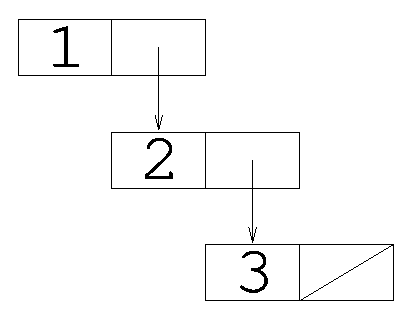
\epsfig{file=cons.ps}}
\end{center}
\end{figure}

List operations are typically implemented in a recursive fashion, where the cdr of the list is taken until the desired element is reached.

\wordtable{
\classword{general-list}{lists}\\
\classword{list}{lists}
}
A \emph{general list} is either the empty list or a cons cell. A \emph{list} is either the empty list or a cons cell whose cdr is also a list. A list is sometimes also known as a \emph{proper list}, and a general list that is not a proper list is known as a \texttt{improper list}. Not all list operations will function given an improper list,
however methods are usually defined on \texttt{general-list} not \texttt{list} since dispatching on \texttt{list} involves a costly check.

\subsubsection{List operations}

\wordtable{
\ordinaryword{>list}{>list ( sequence -- list )}{lists}
}
Turn an arbitrary sequence into a list.
\wordtable{
\ordinaryword{list?}{list?~( obj -- ?~)}{lists}
}
Tests if the object at the top of the stack is a proper list.
\wordtable{
\ordinaryword{unit}{unit ( obj -- [ obj ] )}{lists}
}
Makes a list of one element.
\wordtable{
\ordinaryword{2list}{2list ( o1 o2 -- [ o1 o2 ] )}{lists}
}
Makes a list of two elements.
\wordtable{
\ordinaryword{2unlist}{2unlist ( [ o1 o2 ] -- o1 o2 )}{lists}
}
Pushes the first two elements of a list.
\wordtable{
\ordinaryword{3list}{3list ( o1 o2 o3 -- [ o1 o2 o3 ] )}{lists}
}
Makes a list of three elements.
\wordtable{
\ordinaryword{3unlist}{3unlist ( [ o1 o2 o3 ] -- o1 o2 o3 )}{lists}
}
Pushes the first three elements of a list.
\wordtable{
\ordinaryword{unique}{unique ( obj list -- list )}{lists}
}
If the list already contains an element equal to the object, do nothing, otherwise cons the object into the list.
\wordtable{
\ordinaryword{prune}{prune ( list -- list )}{lists}
}
Removes all duplicates from the list by testing elements for equality.
\wordtable{
\ordinaryword{all=?}{all=?~( list -- ?~)}{lists}
}
Tests if all elements of the list are equal. For the empty list, this is vacuously true.
\wordtable{
\ordinaryword{head}{head~( list n -- list )}{lists}
}
Outputs a new list consisting of the first \texttt{n} elements of \texttt{list}. This allocates memory.
\wordtable{
\ordinaryword{tail}{tail~( list n -- list )}{lists}
}
Outputs a new list consisting of the elements of \texttt{list} from the $n$th index onward. This does not allocate memory; rather it simply takes the \texttt{cdr} \texttt{n} times.
\wordtable{
\ordinaryword{count}{count~( n -- list )}{lists}
}
Return a new list containing all integers from 0 up to $n-1$, inclusive.

\subsubsection{Set-theoretic operations}

\wordtable{
\ordinaryword{contains?}{contains?~( object list -- ?~)}{lists}
}
Tests if \texttt{list} contains an element equal to \texttt{object}.
\wordtable{
\ordinaryword{memq?}{memq?~( object list -- ?~)}{lists}
}
Tests if \texttt{list} contains \texttt{object}. Elements are compared by identity.
\wordtable{
\ordinaryword{contained?}{contained?~( l1 l2 -- ?~)}{lists}
}
Tests if every element of \texttt{l1} is equal to some element of \texttt{l2}.
\wordtable{
\ordinaryword{remove}{remove ( object list -- list )}{lists}
}
Outputs a new list containing all elements of the \texttt{list} except those equal to the \texttt{object}.
\wordtable{
\ordinaryword{remq}{remove ( object list -- list )}{lists}
}
Outputs a new list containing all elements of the \texttt{list} except \texttt{object}. Elements are compared by identity.
\wordtable{
\ordinaryword{intersection}{intersection ( list list -- list )}{lists}
}
Outputs a list of elements present in both lists.
\wordtable{
\ordinaryword{intersection}{difference ( l1 l2 -- list )}{lists}
}
Outputs a list of elements present in \texttt{l2} but not \texttt{l1}.

\subsubsection{List combinators}

\wordtable{
\ordinaryword{each}{each ( list quot -- )}{lists}\\
\texttt{quot:~element --}
}
Applies the quotation to each element of the list.
\wordtable{
\ordinaryword{map}{map ( list quot -- list )}{lists}\\
\texttt{quot:~element -- element}
}
Applies the quotation to each element yielding a new element. The new elements are collected into a new list.
\wordtable{
\ordinaryword{subset}{subset ( list quot -- list )}{lists}\\
\texttt{quot:~element -- ?}
}
Applies the quotation to each element, and outputs a new list containing the elements of the original list for which the quotation output true.
\wordtable{
\ordinaryword{some?}{some?~( list quot -- list )}{lists}\\
\texttt{quot:~element -- ?}
}
Applies the quotation to each element, and outputs the rest of the list upon encountering an element for which the quotation outputs true. If the quotation did not output true for any element, \texttt{some?}~outputs \texttt{f}. Note that the output is a generalized boolean; if the quotation matched any element, the result is true.
\wordtable{
\ordinaryword{all?}{all?~( list quot -- list )}{lists}\\
\texttt{quot:~element -- ?}
}
Outputs \texttt{t} if the quotation yields true when applied to each element, otherwise outputs \texttt{f}. Given the empty list, vacuously outputs \texttt{t}.
\wordtable{
\ordinaryword{sort}{all?~( list quot -- list )}{lists}\\
\texttt{quot:~e1 e2 -- ?}
}
Sorts the list by comparing each pair of elements with the quotation. The quotation should output \texttt{t} if \texttt{e2} is to come before \texttt{e1} in the list. For example, to sort a list of numbers in ascending order, you can do the following:
\begin{alltt}
\textbf{ok} [ 8 6 9 1 10 3 ] [ > ] sort .
[ 1 3 6 8 9 10 ]
\end{alltt}
\wordtable{
\ordinaryword{each-with}{each-with ( object list quot -- )}{lists}\\
\texttt{quot:~object element --}\\
\ordinaryword{map-with}{map-with ( object list quot -- list )}{lists}\\
\texttt{quot:~object element -- element}\\
\ordinaryword{subset-with}{subset-with ( object list quot -- list )}{lists}\\
\texttt{quot:~object element -- ?}\\
\ordinaryword{some-with?}{some-with?~( object list quot -- ?~)}{lists}\\
\texttt{quot:~object element -- ?}\\
\ordinaryword{all-with?}{all-with?~( object list quot -- ?~)}{lists}\\
\texttt{quot:~object element -- ?}
}
Curried forms of the above combinators. They pass an additional object to each invocation of the quotation.

\subsubsection{Queues}

The following set of words manages LIFO (last-in-first-out) queues. Queues are built up from cons cells, and hence are immutable; queue operations always return a new queue.

\wordtable{
\ordinaryword{<queue>}{<queue> ( -- queue )}{lists}
}
Makes a new queue with no elements.
\wordtable{
\ordinaryword{queue-empty?}{queue-empty? ( queue -- ?~)}{lists}
}
Outputs \texttt{t} if the given queue does not contain any elements, \texttt{f} otherwise.
\wordtable{
\ordinaryword{deque}{deque ( queue -- element queue )}{lists}
}
Dequeues an element and outputs a new queue without that element.
\wordtable{
\ordinaryword{enque}{deque ( element queue -- queue )}{lists}
}
Enqueues an element and outputs a new queue.

\subsection{Strings}

\stringglos
\wordtable{
\classword{string}{strings}
}
A string is an immutable sequence of characters. The literal syntax is covered in \ref{string-literals}. Characters do not have a distinct data type, so elements taken out of strings appear as integers on the stack.

\wordtable{
\ordinaryword{string?}{string?~( obj -- ?~)}{strings}
}
Tests if the object at the top of the stack is a string.
%\wordtable{
%\ordinaryword{>string}{>string~( sequence -- string )}{strings}
%}
%Turns any type of sequence with all-integer elements into a string. The integer elements are interpreted as characters.
\wordtable{
\ordinaryword{string-compare}{string-compare~( s1 s2 -- n )}{strings}
}
Compare two strings lexicographically (dictionary order). The output value is one of the following:
\begin{description}
\item[Positive] indicating that \texttt{s1} follows \texttt{s2}
\item[Zero] indicating that \texttt{s1} is equal to \texttt{s2}
\item[Negative] indicating that \texttt{s1} precedes \texttt{s2}
\end{description}
\wordtable{
\ordinaryword{string>}{string> ( s1 s2 -- ?~)}{strings}
}
Tests if \texttt{s1} follows \texttt{s2}. Implemented as follows:
\begin{verbatim}
: string> ( s1 s1 -- ? ) string-compare 0 > ;
\end{verbatim}
This is used to sort lists of strings:
\begin{alltt}
\textbf{ok} [ "Curry" "Apple" "Veal" "Turkey" ] [ string> ] sort .
[ "Apple" "Curry" "Turkey" "Veal" ]
\end{alltt}
\wordtable{
\ordinaryword{fill}{fill~( n char -- string )}{strings}
}
Creates a string with \texttt{char} repeated $n$ times.
\wordtable{
\ordinaryword{pad}{pad~( string n char -- string )}{strings}
}
Creates a string with \texttt{char} repeated $l-n$ times, where $l$ is the length of \texttt{string}. If $l$ is greater than $n$, the empty string is output.

\subsubsection{Substring testing}

\wordtable{
\ordinaryword{string-contains?}{string-contains?~( s1 s2 -- ?~)}{strings}
}
Tests if \texttt{s2} contains \texttt{s1} as a substring.
\wordtable{
\ordinaryword{string-head?}{string-head?~( s1 s2 -- ?~)}{strings}\\
\ordinaryword{string-tail?}{string-tail?~( s1 s2 -- ?~)}{strings}
}
Tests if \texttt{s1} starts or ends with \texttt{s1} as a substring. If \texttt{s1} is longer than \texttt{s2}, outputs \texttt{f}.

\subsubsection{Slicing and splitting}

\wordtable{
\ordinaryword{string/}{string/ ( string n -- s1 s2 )}{strings}
}
Outputs a pair of strings that equal the original string when concatenated. The first string has length $n$, the second has length $l-n$ where $l$ is the length of the input.
\begin{alltt}
\textbf{ok} "Hello world" 5 string .s
\textbf{" world"
"Hello"}
\end{alltt}
\wordtable{
\ordinaryword{string//}{string// ( string n -- s1 s2 )}{strings}
}

Outputs a pair of strings that equal the original string, excluding the $n$th element, when concatenated. The first string has length $n$, the second has length $l-n$ where $l$ is the length of the input.
\begin{alltt}
\textbf{ok} "Hello world" 5 string// .s
\textbf{"world"
"Hello"}
\end{alltt}
\wordtable{
\ordinaryword{?string-head}{?string-head~( s1 s2 -- string ?~)}{strings}\\
\ordinaryword{?string-tail}{?string-tail~( s1 s2 -- string ?~)}{strings}
}
Tests if \texttt{s1} starts or ends with \texttt{s1} as a substring. If there is a match, outputs the subrange of \texttt{s1} excluding \texttt{s1} followed by \texttt{t}. If there is no match, outputs \texttt{s1} followed by \texttt{f}/
\wordtable{
\ordinaryword{split1}{split1~( str split -- before after )}{strings}
}
If \texttt{string} does not contain \texttt{split} as a substring, then \texttt{before} is equal to the \texttt{string}, and \texttt{after} is \texttt{f}. Otherwise, \texttt{before} and \texttt{after} are both strings, and yield the input excluding \texttt{split} when concatenated.
\wordtable{
\ordinaryword{split}{split~( str split -- list )}{strings}
}
Outputs a list of substrings taken between occurrences of \texttt{split} in \texttt{string}. If \texttt{split} does not occur inside \texttt{string}, outputs a singleton list containing \texttt{string} only.
\begin{alltt}
\textbf{ok} "/usr/local/bin" CHAR: / split .
\textbf{[ "" "usr" "local" "bin" ]}
\end{alltt}
\wordtable{
\ordinaryword{split-n}{split-n~( str n -- list )}{strings}
}
Splits the string into groups of \texttt{n} characters and collects them in a list. If the string's length is not a multiple of \texttt{n}, the final string in the list might be shorter.

\subsubsection{Characters}

\wordtable{
\ordinaryword{ch>string}{ch>string ( n -- string )}{strings}
}
Turns an integer representing a character value into a single-element string.
\wordtable{
\ordinaryword{blank?}{blank?~( n -- ?~)}{strings}\\
\ordinaryword{letter?}{letter?~( n -- ?~)}{strings}\\
\ordinaryword{LETTER?}{LETTER?~( n -- ?~)}{strings}\\
\ordinaryword{digit?}{digit?~( n -- ?~)}{strings}\\
\ordinaryword{printable?}{printable?~( n -- ?~)}{strings}\\
\ordinaryword{quotable?}{quotable?~( n -- ?~)}{strings}\\
\ordinaryword{url-quotable?}{url-quotable?~( n -- ?~)}{strings}
}
Various character classification predicates.

\subsection{String buffers}

\sbufglos
\wordtable{
\classword{sbuf}{strings}
}
A string buffer is a mutable and growable sequence of characters. String buffers can be used to construct new strings by accumilating substrings and characters, however usually they are only used indirectly, since the sequence construction words in \ref{make-seq} are more convenient to use in many cases.
\wordtable{
\ordinaryword{sbuf?}{sbuf?~( object -- ?~)}{strings}
}
Tests if the object at the top of the stack is a string buffer.
\wordtable{
\ordinaryword{>sbuf}{>sbuf~( sequence -- sbuf )}{strings}
}
Turns any type of sequence into a string buffer. Given a string buffer, this makes a fresh copy
\wordtable{
\ordinaryword{sbuf>string}{sbuf>string~( sbuf -- string )}{strings}
}
Turns a string buffer into a string holding the same characters.

\subsection{\label{make-seq}Constructing sequences}

The library supports an idiom where sequences can be constructed without passing the partial sequence being built on the stack. This reduces stack noise, and thus simplifies code and makes it easier to understand.

\newcommand{\dynamicscopeglos}{\glossary{
name=dynamic scope,
description={a variable binding policy where bindings established in a scope are visible to all code executed while the scope is active}}}
\dynamicscopeglos
\wordtable{
\ordinaryword{make-list}{make-list ( quot -- list )}{namespaces}\\
\ordinaryword{make-string}{make-string ( quot -- string )}{namespaces}\\
\ordinaryword{make-sbuf}{make-sbuf ( quot -- string )}{namespaces}\\
\ordinaryword{make-vector}{make-vector ( quot -- vector )}{namespaces}
}
Calls the quotation in a new \texttt{dynamic scope}. The quotation and any words it calls can execute the \texttt{,} and \texttt{\%} words to add elements at the end of the sequence being constructed.
\wordtable{
\ordinaryword{,}{,~( element -- )}{namespaces}
}
Adds the element to the end of the sequence being constructed by the innermost call to one of the above combinators.
\wordtable{
\ordinaryword{unique,}{unique,~( element -- )}{namespaces}
}
Adds the element to the end of the sequence being constructed as long as the sequence does not already have an equal element.
\wordtable{
\ordinaryword{literal,}{literal,~( element -- )}{namespaces}
}
Adds the element wrapped inside a one-element list, then adds the \texttt{car} word. This is used to construct quotations with \texttt{make-list} that must push a word on the stack.
\wordtable{
\ordinaryword{\%}{\% ( sequence -- )}{namespaces}
}
Appends the subsequence to the end of the sequence being constructed.

Note that the sequence construction combinators will capture any variables set inside the quotation, due to the dynamic scoping behavior. These combinators are actually implemented using variables. See \ref{namespaces}.

\section{Mappings}

\glossary{name=mapping,
description={an unordered collection of elements, accessed by key. Examples include association lists and hashtables}}

Mappings associate keys with values. The two classes of mappings in the Factor library are association lists and hashtables.

\begin{tabular}[t]{l|c|c|c|l}
Class&Mutable&Ordered&Lookup&Primary purpose\\
\hline
\texttt{assoc}&&$\surd$&$O(n)$&Small, unchanging mappings\\
\texttt{hashtable}&$\surd$&&$O(1)$&Large or frequently-changing mappings
\end{tabular}

It might be tempting to just always use hashtables, however for very small mappings, association lists are just as efficient, and are easier to work with since the entire set of list words can be used with them.

\subsection{Association lists}

\glossary{name=association list,
description={a list of pairs, where the car if each pair is a key and the cdr is the value associated with that key}}

Association lists are built from cons cells. They are structured like a ribbed spine, where the ``spine'' is a list and each ``rib'' is a cons cell holding a key/value pair.

\wordtable{
\ordinaryword{assoc?}{assoc ( object -- ?~)}{lists}
}
Tests if the object at the top of the stack is a proper list whose every element is a cons.

\wordtable{
\ordinaryword{assoc}{assoc ( k alist -- v )}{lists}\\
\ordinaryword{assoc*}{assoc* ( k alist -- [[ k v ]] )}{lists}
}
These words look up a key in an association list, comparing keys in the list with the given key by equality with \texttt{=}. The list is searched starting from the beginning. The two words differ in that the latter returns the key/value pair located, whereas the former only returns the value. The \texttt{assoc*} word allows a distinction to be made between a missing value and a value equal to \texttt{f}, since in the case of a missing value it outputs \texttt{f}.
\wordtable{
\ordinaryword{assq}{assq ( k alist -- v )}{lists}\\
\ordinaryword{assq*}{assq* ( k alist -- [[ k v ]] )}{lists}
}
These words compare keys by identity with \texttt{eq?}~and are dual to \texttt{assoc} and \texttt{assoc*}.
\wordtable{
\ordinaryword{acons}{acons ( v k alist -- alist )}{lists}\\
\ordinaryword{set-assoc}{set-assoc ( v k alist -- alist )}{lists}
}
These words output a new association list containing the key/value pair.
They differ in that \texttt{set-assoc} removes any existing key/value pairs with the given key first. In both cases, searching for the key in the returned association list gives the new value, however with the slightly faster \texttt{acons}, the old value remains shadowed in the list.
\wordtable{
\ordinaryword{remove-assoc}{remove-assoc ( k alist -- alist )}{lists}
}
Outputs a new association list which does not have any key/value pairs with the key equal to \texttt{k}.

\begin{figure}
\caption{An association list and its graphical representation}
\begin{verbatim}
[
    [[ "Salsa" "Hot" ]]
    [[ "Stir-Fry" "Medium" ]]
    [[ "Peppers" "Very Hot" ]]
]
\end{verbatim}

\begin{center}
\scalebox{0.45}{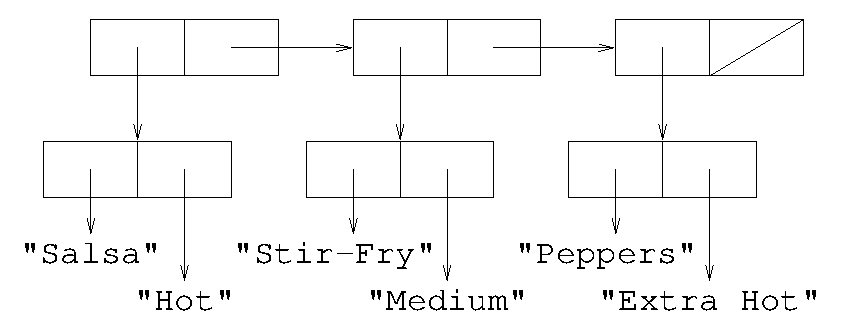
\epsfig{file=assoc.eps}}
\end{center}
\end{figure}

\subsubsection{Dual representation}

Sometimes it is convenient to decompose an association list into two lists of equal length, containing the keys and values, respectively, in the same order as the association list. This dual representation can be manipulated with a handful of helper words.

\wordtable{
\ordinaryword{zip}{zip ( keys values -- alist )}{lists}\\
\ordinaryword{unzip}{unzip ( alist -- keys values )}{lists}
}
These words convert between pairs of lists and lists of pairs.
\begin{alltt}
\textbf{ok} [ 1 2 3 ] [ 4 5 6 ] zip .
[ [[ 1 4 ]] [[ 2 5 ]] [[ 3 6 ]] ]
\textbf{ok} [ [[ 1 2 ]] [[ 3 4 ]] [[ 5 6 ]] ] unzip .s
[ 2 4 6 ]
[ 1 3 5 ]
\end{alltt}
\wordtable{
\ordinaryword{2cons}{2cons ( car1 car2 cdr1 cdr2 -- c1 c2 )}{lists}
}
Cons a pair of elements onto a pair of lists.
\wordtable{
\ordinaryword{2car}{2car ( c1 c2 -- car1 car2 )}{lists}\\
\ordinaryword{2cdr}{2cdr ( c1 c2 -- cdr1 cdr2 )}{lists}
}
Deconstructs paired lists.

\subsection{Hashtables}

\wordtable{
\classword{hashtable}{hashtables}
}


\subsection{\label{namespaces}Namespaces}

\section{Mathematics}

\numberglos

\begin{figure}
\begin{center}
\caption{Numerical class hierarchy}
\scalebox{0.5}{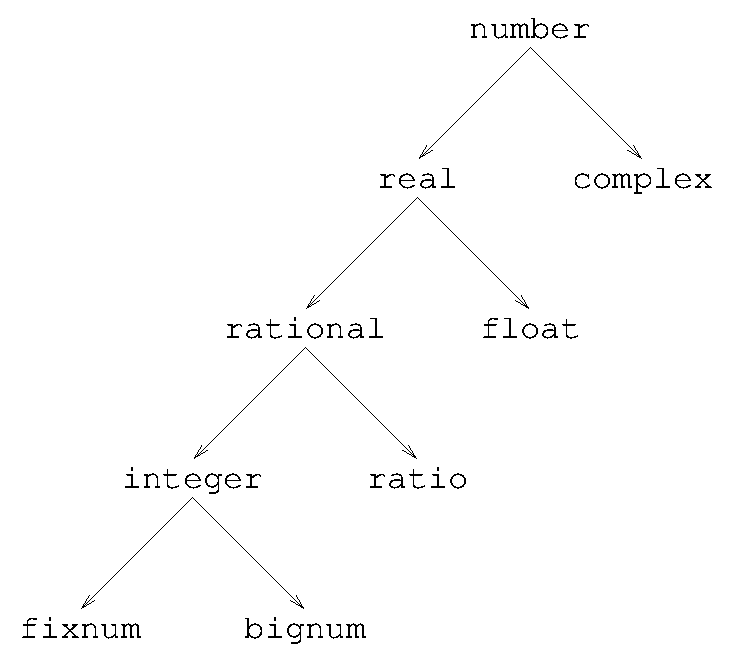
\epsfig{file=number.ps}}
\end{center}
\end{figure}

Factor's numbers more closely model the mathematical concept of a number than other languages. Where possible, exact answers are given -- for example, adding or multiplying two integers never results in overflow, and dividing two integers yields a fraction rather than a truncated result. Complex numbers are supported, allowing many functions to be computed with parameters that would raise errors or return ``not a number'' in other languages.

\subsection{Integers}

\integerglos

The simplest type of number is the integer. Integers come in two varieties -- \emph{fixnums} and \emph{bignums}. As their names suggest, a fixnum is a fixed-width quantity\footnote{Fixnums range in size from $-2^{w-3}-1$ to $2^{w-3}$, where $w$ is the word size of your processor (for example, 32 bits). Because fixnums automatically grow to bignums, usually you do not have to worry about details like this.}, and is a bit quicker to manipulate than an arbitrary-precision bignum.

The predicate word \texttt{integer?}~tests if the top of the stack is an integer. If this returns true, then exactly one of \texttt{fixnum?}~or \texttt{bignum?}~would return true for that object. Usually, your code does not have to worry if it is dealing with fixnums or bignums.

Unlike some languages where the programmer has to declare storage size explicitly and worry about overflow, integer operations automatically return bignums if the result would be too big to fit in a fixnum. Here is an example where multiplying two fixnums returns a bignum:

\begin{alltt}
\textbf{ok} 134217728 fixnum? .
\textbf{t}
\textbf{ok} 128 fixnum? .
\textbf{t}
\textbf{ok} 134217728 128 * .
\textbf{17179869184}
\textbf{ok} 134217728 128 * bignum? .
\textbf{t}
\end{alltt}

Integers can be entered using a different base. By default, all number entry is in base 10, however this can be changed by prefixing integer literals with one of the parsing words \texttt{BIN:}, \texttt{OCT:}, or \texttt{HEX:}. For example:

\begin{alltt}
\textbf{ok} BIN: 1110 BIN: 1 + .
\textbf{15}
\textbf{ok} HEX: deadbeef 2 * .
\textbf{7471857118}
\end{alltt}

The word \texttt{.} prints numbers in decimal, regardless of how they were input. A set of words in the \texttt{prettyprint} vocabulary is provided for print integers using another base.

\begin{alltt}
\textbf{ok} 1234 .h
\textbf{4d2}
\textbf{ok} 1234 .o
\textbf{2232}
\textbf{ok} 1234 .b
\textbf{10011010010}
\end{alltt}

\subsection{Rational numbers}

\newcommand{\rationalglos}{\glossary{
name=rational,
description={an instance of the \texttt{rational} class, which is a disjoint union of the
\texttt{integer} and \texttt{ratio} classes}}}
\rationalglos
\ratioglos

If we add, subtract or multiply any two integers, the result is always an integer. However, this is not the case with division. When dividing a numerator by a denominator where the numerator is not a integer multiple of the denominator, a ratio is returned instead.

\begin{alltt}
1210 11 / .
\emph{110}
100 330 / .
\emph{10/33}
\end{alltt}

Ratios are printed and can be input literally in the form of the second example. Ratios are always reduced to lowest terms by factoring out the greatest common divisor of the numerator and denominator. A ratio with a denominator of 1 becomes an integer. Trying to create a ratio with a denominator of 0 raises an error.

The predicate word \texttt{ratio?}~tests if the top of the stack is a ratio. The predicate word \texttt{rational?}~returns true if and only if one of \texttt{integer?}~or \texttt{ratio?}~would return true for that object. So in Factor terms, a ``ratio'' is a rational number whose denominator is not equal to 1.

Ratios behave just like any other number -- all numerical operations work as expected, and in fact they use the formulas for adding, subtracting and multiplying fractions that you learned in high school.

\begin{alltt}
\textbf{ok} 1/2 1/3 + .
\textbf{5/6}
\textbf{ok} 100 6 / 3 * .
\textbf{50}
\end{alltt}

Ratios can be deconstructed into their numerator and denominator components using the \texttt{numerator} and \texttt{denominator} words. The numerator and denominator are both integers, and furthermore the denominator is always positive. When applied to integers, the numerator is the integer itself, and the denominator is 1.

\begin{alltt}
\textbf{ok} 75/33 numerator .
\textbf{25}
\textbf{ok} 75/33 denominator .
\textbf{11}
\textbf{ok} 12 numerator .
\textbf{12}
\end{alltt}

\subsection{Floating point numbers}

\newcommand{\realglos}{\glossary{
name=real,
description={an instance of the \texttt{real} class, which is a disjoint union of the
\texttt{rational} and \texttt{float} classes}}}
\realglos
\floatglos

Rational numbers represent \emph{exact} quantities. On the other hand, a floating point number is an \emph{approximation}. While rationals can grow to any required precision, floating point numbers are fixed-width, and manipulating them is usually faster than manipulating ratios or bignums (but slower than manipulating fixnums). Floating point literals are often used to represent irrational numbers, which have no exact representation as a ratio of two integers. Floating point literals are input with a decimal point.

\begin{alltt}
\textbf{ok} 1.23 1.5 + .
\textbf{1.73}
\end{alltt}

The predicate word \texttt{float?}~tests if the top of the stack is a floating point number. The predicate word \texttt{real?}~returns true if and only if one of \texttt{rational?}~or \texttt{float?}~would return true for that object.

Floating point numbers are \emph{contagious} -- introducing a floating point number in a computation ensures the result is also floating point.

\begin{alltt}
\textbf{ok} 5/4 1/2 + .
\textbf{7/4}
\textbf{ok} 5/4 0.5 + .
\textbf{1.75}
\end{alltt}

Apart from contaigion, there are two ways of obtaining a floating point result from a computation; the word \texttt{>float ( n -{}- f )} converts a rational number into its floating point approximation, and the word \texttt{/f ( x y -{}- x/y )} returns the floating point approximation of a quotient of two numbers.

\begin{alltt}
\textbf{ok} 7 4 / >float .
\textbf{1.75}
\textbf{ok} 7 4 /f .
\textbf{1.75}
\end{alltt}

Indeed, the word \texttt{/f} could be defined as follows:

\begin{alltt}
: /f / >float ;
\end{alltt}

However, the actual definition is slightly more efficient, since it computes the floating point result directly.

\subsection{Complex numbers}

Complex numbers arise as solutions to quadratic equations whose graph does not intersect the x axis. For example, the equation $x^2 + 1 = 0$ has no solution for real $x$, because there is no real number that is a square root of -1. However, in the field of complex numbers, this equation has a well-known solution:

\begin{alltt}
\textbf{ok} -1 sqrt .
\textbf{\#\{ 0 1 \}}
\end{alltt}

The literal syntax for a complex number is \texttt{\#\{ re im \}}, where \texttt{re} is the real part and \texttt{im} is the imaginary part. For example, the literal \texttt{\#\{ 1/2 1/3 \}} corresponds to the complex number $1/2 + 1/3i$.

The words \texttt{i} an \texttt{-i} push the literals \texttt{\#\{ 0 1 \}} and \texttt{\#\{ 0 -1 \}}, respectively.

The predicate word \texttt{complex?} tests if the top of the stack is a complex number. Note that unlike math, where all real numbers are also complex numbers, Factor only considers a number to be a complex number if its imaginary part is non-zero.

Complex numbers can be deconstructed into their real and imaginary components using the \texttt{real} and \texttt{imaginary} words. Both components can be pushed at once using the word \texttt{>rect ( z -{}- re im )}.

\begin{alltt}
\textbf{ok} -1 sqrt real .
\textbf{0}
\textbf{ok} -1 sqrt imaginary .
\textbf{1}
\textbf{ok} -1 sqrt sqrt >rect .s
\textbf{\{ 0.7071067811865476 0.7071067811865475 \}}
\end{alltt}

A complex number can be constructed from a real and imaginary component on the stack using the word \texttt{rect> ( re im -{}- z )}.

\begin{alltt}
\textbf{ok} 1/3 5 rect> .
\textbf{\#\{ 1/3 5 \}}
\end{alltt}

Complex numbers are stored in \emph{rectangular form} as a real/imaginary component pair (this is where the names \texttt{>rect} and \texttt{rect>} come from). An alternative complex number representation is \emph{polar form}, consisting of an absolute value and argument. The absolute value and argument can be computed using the words \texttt{abs} and \texttt{arg}, and both can be pushed at once using \texttt{>polar ( z -{}- abs arg )}.

\begin{alltt}
\textbf{ok} 5.3 abs .
\textbf{5.3}
\textbf{ok} i arg .
\textbf{1.570796326794897}
\textbf{ok} \#\{ 4 5 \} >polar .s
\textbf{\{ 6.403124237432849 0.8960553845713439 \}}
\end{alltt}

A new complex number can be created from an absolute value and argument using \texttt{polar> ( abs arg -{}- z )}.

\begin{alltt}
\textbf{ok} 1 pi polar> .
\textbf{\#\{ -1.0 1.224606353822377e-16 \}}
\end{alltt}

\subsection{Transcedential functions}

The \texttt{math} vocabulary provides a rich library of mathematical functions that covers exponentiation, logarithms, trigonometry, and hyperbolic functions. All functions accept and return complex number arguments where appropriate. These functions all return floating point values, or complex numbers whose real and imaginary components are floating point values.

\texttt{\^{} ( x y -- x\^{}y )} raises \texttt{x} to the power of \texttt{y}. In the cases of \texttt{y} being equal to $1/2$, -1, or 2, respectively, the words \texttt{sqrt}, \texttt{recip} and \texttt{sq} can be used instead.

\begin{alltt}
\textbf{ok} 2 4 \^ .
\textbf{16.0}
\textbf{ok} i i \^ .
\textbf{0.2078795763507619}
\end{alltt}

All remaining functions have a stack effect \texttt{( x -{}- y )}, it won't be repeated for brevity.

\texttt{exp} raises the number $e$ to a specified power. The number $e$ can be pushed on the stack with the \texttt{e} word, so \texttt{exp} could have been defined as follows:

\begin{alltt}
: exp ( x -- e^x ) e swap \^ ;
\end{alltt}

However, it is actually defined otherwise, for efficiency.\footnote{In fact, the word \texttt{\^{}} is actually defined in terms of \texttt{exp}, to correctly handle complex number arguments.}

\texttt{log} computes the natural (base $e$) logarithm. This is the inverse of the \texttt{exp} function.

\begin{alltt}
\textbf{ok} -1 log .
\textbf{\#\{ 0.0 3.141592653589793 \}}
\textbf{ok} e log .
\textbf{1.0}
\end{alltt}

\texttt{sin}, \texttt{cos} and \texttt{tan} are the familiar trigonometric functions, and \texttt{asin}, \texttt{acos} and \texttt{atan} are their inverses.

The reciprocals of the sine, cosine and tangent are defined as \texttt{sec}, \texttt{cosec} and \texttt{cot}, respectively. Their inverses are \texttt{asec}, \texttt{acosec} and \texttt{acot}.

\texttt{sinh}, \texttt{cosh} and \texttt{tanh} are the hyperbolic functions, and \texttt{asinh}, \texttt{acosh} and \texttt{atanh} are their inverses.

Similarly, the reciprocals of the hyperbolic functions are defined as \texttt{sech}, \texttt{cosech} and \texttt{coth}, respectively. Their inverses are \texttt{asech}, \texttt{acosech} and \texttt{acoth}.

\subsection{Modular arithmetic}

In addition to the standard division operator \texttt{/}, there are a few related functions that are useful when working with integers.

\texttt{/i ( x y -{}- x/y )} performs a truncating integer division. It could have been defined as follows:

\begin{alltt}
: /i / >integer ;
\end{alltt}

However, the actual definition is a bit more efficient than that.

\texttt{mod ( x y -{}- x\%y )} computes the remainder of dividing \texttt{x} by \texttt{y}. If the result is 0, then \texttt{x} is a multiple of \texttt{y}.

\texttt{/mod ( x y -{}- x/y x\%y )} pushes both the quotient and remainder.

\begin{alltt}
\textbf{ok} 100 3 mod .
\textbf{1}
\textbf{ok} -546 34 mod .
\textbf{-2}
\end{alltt}

\texttt{gcd ( x y -{}- z )} pushes the greatest common divisor of two integers; that is, the largest number that both integers could be divided by and still yield integers as results. This word is used behind the scenes to reduce rational numbers to lowest terms when doing ratio arithmetic.

\subsection{Bitwise operations}

There are two ways of looking at an integer -- as a mathematical entity, or as a string of bits. The latter representation faciliates the so-called \emph{bitwise operations}.

\texttt{bitand ( x y -{}- x\&y )} returns a new integer where each bit is set if and only if the corresponding bit is set in both $x$ and $y$. If you're considering an integer as a sequence of bit flags, taking the bitwise-and with a mask switches off all flags that are not explicitly set in the mask.

\begin{alltt}
BIN: 101 BIN: 10 bitand .b
\emph{0}
BIN: 110 BIN: 10 bitand .b
\emph{10}
\end{alltt}

\texttt{bitor ( x y -{}- x|y )} returns a new integer where each bit is set if and only if the corresponding bit is set in at least one of $x$ or $y$. If you're considering an integer as a sequence of bit flags, taking the bitwise-or with a mask switches on all flags that are set in the mask.

\begin{alltt}
BIN: 101 BIN: 10 bitor .b
\emph{111}
BIN: 110 BIN: 10 bitor .b
\emph{110}
\end{alltt}

\texttt{bitxor ( x y -{}- x\^{}y )} returns a new integer where each bit is set if and only if the corresponding bit is set in exactly one of $x$ or $y$. If you're considering an integer as a sequence of bit flags, taking the bitwise-xor with a mask toggles on all flags that are set in the mask.

\begin{alltt}
BIN: 101 BIN: 10 bitxor .b
\emph{111}
BIN: 110 BIN: 10 bitxor .b
\emph{100}
\end{alltt}

\texttt{bitnot ( x -{}- y )} returns the bitwise complement of the input; that is, each bit in the input number is flipped. This is actually equivalent to negating a number, and subtracting one. So indeed, \texttt{bitnot} could have been defined as thus:

\begin{alltt}
: bitnot neg pred ;
\end{alltt}

\texttt{shift ( x n -{}- y )} returns a new integer consisting of the bits of the first integer, shifted to the left by $n$ positions. If $n$ is negative, the bits are shifted to the right instead, and bits that ``fall off'' are discarded.

\begin{alltt}
BIN: 101 5 shift .b
\emph{10100000}
BIN: 11111 -2 shift .b
\emph{111}
\end{alltt}

The attentive reader will notice that shifting to the left is equivalent to multiplying by a power of two, and shifting to the right is equivalent to performing a truncating division by a power of two.

\chapter{The development environment}

Factor supports interactive development in a live environment. Instead of working with
static executable files and restarting your application after each change, you can
incrementally make changes to your application and test them immediately. If you
notice an undesirable behavior, Factor's powerful reflection features will aid in
pinpointing the error.

If you are used to a statically typed language, you might find Factor's tendency to only fail at runtime hard to work with at first. However, the interactive development tools outlined in this document allow a much quicker turn-around time for testing changes. Also, write unit tests -- unit testing is a great way to ensure that old bugs do not re-appear once they've been fixed.

\section{System organization}

\subsection{The listener}

Factor is an \emph{image-based environment}. When you compiled Factor, you also generated a file named \texttt{factor.image}. I will have more to say about images later, but for now it suffices to understand that to start Factor, you must pass the image file name on the command line:
\begin{alltt}
./f factor.image
\textbf{Loading factor.image... relocating... done
Factor 0.73 :: http://factor.sourceforge.net :: unix/x86
(C) 2003, 2005 Slava Pestov, Chris Double,
Mackenzie Straight
ok}
\end{alltt}
An \texttt{\textbf{ok}} prompt is printed after the initial banner, indicating the listener is ready to execute Factor phrases. The listener is a piece of Factor code, like any other; however, it helps to think of it as the primary interface to the Factor system. The listener reads Factor code and executes it. You can try the classical first program:

\begin{alltt}
\textbf{ok} "Hello, world." print
\textbf{Hello, world.}
\end{alltt}


Multi-line phrases are supported; if there are unclosed brackets, the listener outputs \texttt{...} instead of the \texttt{ok} prompt, and the entire phrase is executed once all brackets are closed:

\begin{alltt}
\textbf{ok} [ 1 2 3 ] [
\textbf{...} .
\textbf{...} ] each
\textbf{1
2
3}
\end{alltt}

The listener knows when to print a continuation prompt by looking at the height of the
stack. Parsing words such as \texttt{[} and \texttt{:} leave elements on the parser
stack; these elements are popped by \texttt{]} and \texttt{;}.

\subsection{Source files}

While it is possible to do all development in the listener and save your work in images, it is far more convenient to work with source files, at least until an in-image structure editor is developed.

By convention, Factor source files are saved with the \texttt{.factor} filename extension. They can be loaded into the image as follows:

\begin{alltt}
\textbf{ok} "examples/numbers-game.factor" run-file
\end{alltt}

In Factor, loading a source file replaces any existing definitions\footnote{But see \ref{compiler} for this is not true of compiled code.}. Each word definition remembers what source file it was loaded from (if any). To reload the source file associated with a definition, use the \texttt{reload} word:

\begin{alltt}
\textbf{ok} \bs draw reload
\end{alltt}

Word definitions also retain the line number where they are located in their original source file. This allows you to open a word definition in jEdit\footnote{\texttt{http://www.jedit.org}} for editing using the
\texttt{jedit} word:

\begin{alltt}
\textbf{ok} \bs compile jedit
\end{alltt}

This word requires that a jEdit instance is already running.

For the \texttt{jedit} word to work with words in the Factor library, you must set the \texttt{"resource-path"} variable to the location of the Factor source tree. One way to do this is to add a phrase like the following to your \texttt{.factor-rc}:

\begin{verbatim}
"/home/slava/Factor/" "resource-path" set
\end{verbatim}

On startup, Factor reads the \texttt{.factor-rc} file from your home directory. You can put
any quick definitions you want available at the listener there. To avoid loading this
file, pass the \texttt{-no-user-init} command line switch. Another way to have a set of definitions available at all times is to save a custom image, as described in the next section.

\subsection{Images}

The \texttt{factor.image} file is basically a dump of all objects in the heap. A new image can be saved as follows:

\begin{alltt}
\textbf{ok} "work.image" save-image
\textbf{Saving work.image...}
\end{alltt}

When you save an image before exiting Factor, then start Factor again, everything will be almost as you left it. Try the following:

\begin{alltt}
./f factor.image
\textbf{ok} "Learn Factor" "reminder" set
\textbf{ok} "factor.image" save-image bye
\textbf{Saving factor.image...}
\end{alltt}

Factor will save the image and exit. Now start it again and see that the reminder is still there:

\begin{alltt}
./f factor.image
\textbf{ok} "reminder" get .
\textbf{"Learn Factor"}
\end{alltt}

This is what is meant by the image being an \emph{infinite session}. When you shut down and restart Factor, what happends is much closer to a Laptop's ``suspend'' mode, than a desktop computer being fully shut down.

\subsection{Looking at objects}

Probably the most important debugging tool of them all is the \texttt{.} word. It prints the object at the top of the stack in a form that can be parsed by the Factor parser. A related word is \texttt{prettyprint}. It is identical to \texttt{.} except the output is more verbose; lists, vectors and hashtables are broken up into multiple lines and indented.

\begin{alltt}
\textbf{ok} [ [ \tto 1 \ttc \tto 2 \ttc ] dup car swap cdr ] .
[ [ \tto 1 \ttc \tto 2 \ttc ] dup car swap cdr ]
\end{alltt}

Most objects print in a parsable form, but not all. One exceptions to this rule is objects with external state, such as I/O ports or aliens (pointers to native structures). Also, objects with circular or very deeply nested structure will not print in a fully parsable form, since the prettyprinter has a limit on maximum nesting. Here is an example -- a vector is created, that holds a list whose first element is the vector itself:

\begin{alltt}
\textbf{ok} \tto \ttc [ unit 0 ] keep [ set-vector-nth ] keep .
\tto [ ... ] \ttc
\end{alltt}

The prettyprinted form of a vector or list with many elements is not always readable. The \texttt{[.]} and \texttt{\tto.\ttc} words output a list or a vector, respectively, with each element on its own line. In fact, the stack printing words are defined in terms of \texttt{[.]} and \texttt{\tto.\ttc}:

\begin{verbatim}
: .s datastack  {.} ;
: .r callstack  {.} ;
: .n namestack  [.] ;
: .c catchstack [.] ;
\end{verbatim}

Before we move on, one final set of output words comes is used to output integers in
different numeric bases. The \texttt{.b} word prints an integer in binary, \texttt{.o} in octal, and \texttt{.h} in hexadecimal.

\begin{alltt}
\textbf{ok} 31337 .b
\textbf{111101001101001}
\textbf{ok} 31337 .o
\textbf{75151}
\textbf{ok} 31337 .h
\textbf{7a69}
\end{alltt}

\section{Word tools}

\subsection{Exploring vocabularies}

Factor organizes code in a two-tier structure of vocabularies and words. A word is the smallest unit of code; it corresponds to a function or method in other languages. Vocabularies group related words together for easy browsing and tracking of source dependencies.

Entering \texttt{vocabs .}~in the listener produces a list of all existing vocabularies:

\begin{alltt}
\textbf{ok} vocabs .
\textbf{[ "alien" "ansi" "assembler" "browser-responder"
"command-line" "compiler" "cont-responder" "errors"
"file-responder" "files" "gadgets" "generic"
"hashtables" "html" "httpd" "httpd-responder" "image"
"inference" "interpreter" "io-internals" "jedit"
"kernel" "kernel-internals" "line-editor" "listener"
"lists" "logging" "math" "math-internals" "memory"
"namespaces" "parser" "prettyprint" "profiler"
"quit-responder" "random" "resource-responder"
"scratchpad" "sdl" "shells" "stdio" "streams"
"strings" "syntax" "telnetd" "test" "test-responder"
"threads" "unparser" "url-encoding" "vectors" "words" ]}
\end{alltt}

As you can see, there are a lot of vocabularies! Now, you can use \texttt{words .}~to list the words inside a given vocabulary:

\begin{alltt}
\textbf{ok} "namespaces" words .
\textbf{[ (get) , <namespace> >n append, bind change cons@
dec extend get global inc init-namespaces list-buffer
literal, make-list make-rlist make-rstring make-string
make-vector n> namespace namestack nest off on put set
set-global set-namestack unique, unique@ with-scope ]}
\end{alltt}

You can look at the definition of any word, including library words, using \texttt{see}. Keep in mind you might have to \texttt{USE:} the vocabulary first.

\begin{alltt}
\textbf{ok} USE: httpd
\textbf{ok} \bs httpd-connection see
\textbf{IN: httpd : httpd-connection ( socket -- )
    "http-server" get accept [
        httpd-client
    ] in-thread drop ;}
\end{alltt}

The \texttt{see} word shows a reconstruction of the source code, not the original source code. So in particular, formatting and some comments are lost.

\subsection{Cross-referencing words}

The \texttt{apropos.} word is handy when searching for related words. It lists all words
whose names contain a given string. The \texttt{apropos.} word is also useful when you know the exact name of a word, but are unsure what vocabulary it is in. For example, if you're looking for ways to iterate over various collections, you can do an apropos search for \texttt{map}:

\begin{alltt}
\textbf{ok} "map" apropos.
\textbf{IN: inference
type-value-map
IN: lists
map
map-with
IN: sdl
set-surface-map
surface-map
IN: strings
string-map
IN: vectors
vector-map}
\end{alltt}

From the above output, you can see that \texttt{map} is for lists, \texttt{string-map} is for strings, and \texttt{vector-map} is for vectors.

The \texttt{usage} word finds all words that refer to a given word and pushes a list on the stack. This word is helpful in two situations; the first is for learning -- a good way to learn a word is to see it used in context. The second is during refactoring -- if you change a word's stack effect, you must also update all words that call it. Usually you print the
return value of \texttt{usage} using \texttt{.}:

\begin{alltt}
\textbf{ok} \bs string-map usage .
\textbf{schars>entities
filter-null
url-encode}
\end{alltt}

Another useful word is \texttt{usages}. Unlike \texttt{usage}, it finds all usages, even
indirect ones -- so if a word refers to another word that refers to the given word,
both words will be in the output list.

\subsection{Exploring classes}

Factor supports object-oriented programming via generic words. Generic words are called
like ordinary words, however they can have multiple definitions, one per class, and
these definitions do not have to appear in the same source file. Such a definition is
termed a \emph{method}, and the method is said to \emph{specialize} on a certain
class. A class in the most
general sense is just a set of objects. You can output a list of classes in the system
with \texttt{classes .}:

\begin{alltt}
\textbf{ok} classes.
\textbf{[ alien alien-error byte-array displaced-alien
dll ansi-stream disp-only displaced indirect operand
register absolute absolute-16/16 relative relative-bitfld
item kernel-error no-method border checkbox dialog editor
ellipse etched-rect frame gadget hand hollow-ellipse
hollow-rect label line menu pane pile plain-ellipse
plain-rect rectangle roll-rect scroller shelf slider
stack tile viewport world 2generic arrayed builtin
complement generic null object predicate tuple
tuple-class union hashtable html-stream class-tie
computed inference-error inference-warning literal
literal-tie value buffer port jedit-stream boolean
general-t array cons general-list list bignum complex
fixnum float integer number ratio rational real
parse-error potential-float potential-ratio
button-down-event button-up-event joy-axis-event
joy-ball-event joy-button-down-event joy-button-up-event
joy-hat-event key-down-event key-up-event motion-event
quit-event resize-event user-event sequence stdio-stream
client-stream fd-stream null-stream server string-output
wrapper-stream LETTER blank digit letter printable sbuf
string text POSTPONE: f POSTPONE: t vector compound
primitive symbol undefined word ]}
\end{alltt}

If you \texttt{see} a generic word, all methods defined on the generic word are shown.
Alternatively, you can use \texttt{methods.} to print all methods specializing on a
given class:

\begin{alltt}
\textbf{ok} \bs list methods.
\textbf{PREDICATE: general-list list
    dup [
        last* cdr
    ] when not ;
IN: gadgets
M: list custom-sheet
    [
        length count
    ] keep zip alist>sheet "Elements:" <titled> ;
IN: prettyprint
M: list prettyprint*
    [
        [
            POSTPONE: [
        ] car swap [
            POSTPONE: ]
        ] car prettyprint-sequence
    ] check-recursion ;}
\end{alltt}

\subsection{Browsing via the HTTP server}


A more sophisticated way to browse the library is using the integrated HTTP server. You can start the HTTP server using the following pair of commands:

\begin{alltt}
\textbf{ok} USE: httpd
\textbf{ok} 8888 httpd
\end{alltt}

Then, point your browser to the following URL, and start browsing:

\begin{quote}
\texttt{http://localhost:8888/responder/inspect/vocabularies}
\end{quote}

To stop the HTTP server, point your browser to

\begin{quote}
\texttt{http://localhost:8888/responder/quit}.
\end{quote}

You can even start the HTTP in a separate thread, and look at code in your web browser while continuing to play in the listener:

\begin{alltt}
\textbf{ok} USE: httpd
\textbf{ok} USE: threads
\textbf{ok} [ 8888 httpd ] in-thread
\end{alltt}

\section{Dealing with runtime errors}

\subsection{Looking at stacks}

To see the contents of the data stack, use the \texttt{.s} word. Similarly, the other stacks can be shown with \texttt{.r} (return stack), \texttt{.n} (name stack), and \texttt{.c} (catch stack). Each stack is printed with each element on its own line; the top of the stack is the first element printed.

\subsection{The debugger}

If the execution of a phrase in the listener causes an error to be thrown, the error
is printed and the stacks at the time of the error are saved. If you're spent any
time with Factor at all, you are probably familiar with this type of message:

\begin{alltt}
\textbf{ok} [ 1 2 3 ] 4 append reverse
\textbf{The generic word car does not have a suitable method for 4
:s :r :n :c show stacks at time of error.
:get ( var -- value ) inspects the error namestack.}
\end{alltt}

The words \texttt{:s}, \texttt{:r}, \texttt{:n} and \texttt{:s} behave like their counterparts that are prefixed with \texttt{.}, except they show the stacks as they were when the error was thrown.

The return stack warrants some special attention. To successfully develop Factor, you will need to learn to understand how it works. Lets look at the first few lines of the return stack at the time of the above error:

\begin{verbatim}
[ swap cdr ]
uncons
[ r> tuck 2slip ]
(each)
[ swons ]
[ each ]
each
\end{verbatim}

You can see the sequence of calls leading up to the error was \texttt{each} calling \texttt{(each)} calling \texttt{uncons}. The error tells us that the \texttt{car} word is the one that failed. Now, you can stare at the stack dump, at notice that if the call to \texttt{car} was successful and execution returned to \texttt{(each)}, the quotation \texttt{[ r> tuck 2slip ]} would resume executing. The first word there, \texttt{r>}, would take the quotation \texttt{[ swons ]} and put it back on the data stack. After \texttt{(each)} returned, it would then continue executing the quotation \texttt{[ each ]}. So what is going on here is a recursive loop, \texttt{[ swons ] each}. If you look at the definition of \texttt{reverse}, you will see that this is exactly what is being done:

\begin{verbatim}
: reverse ( list -- list ) [ ] swap [ swons ] each ;
\end{verbatim}

So a list is being reversed, but at some stage, the \texttt{car} is taken of something that is not a number. Now, you can look at the data stack with \texttt{:s}:

\begin{verbatim}
<< no-method [ ] 4 car >>
car
4
4
[ 3 2 1 ]
\end{verbatim}

So now, the mystery has been solved: as \texttt{reverse} iterates down the input value, it hits a cons cells whose \texttt{cdr} is not a list. Indeed, if you look at the value we are passing to \texttt{reverse}, you will see why:

\begin{alltt}
\textbf{ok} [ 1 2 3 ] 4 append .
[[ 1 [[ 2 [[ 3 4 ]] ]] ]]
\end{alltt}

In the future, the debugger will be linked with the walker, documented below. Right now, the walker is a separate tool. Another caveat is that in compiled code, the return stack is not reconstructed if there is an error. Until this is fixed, you should only compile code once it is debugged. For more potential compiler pitfalls, see \ref{compiler}.

\subsection{The walker}

The walker lets you step through the execution of a qotation. When a compound definition is reached, you can either keep walking inside the definition, or execute it in one step. The stacks can be inspected at each stage.

There are two ways to use the walker. First of all, you can call the \texttt{walk} word explicitly, giving it a quotation:

\begin{alltt}
\textbf{ok} [ [ 10 [ dup , ] repeat ] make-list ] walk
\textbf{\&s \&r \&n \&c show stepper stacks.
\&get ( var -- value ) inspects the stepper namestack.
step -- single step over
into -- single step into
continue -- continue execution
bye -- exit single-stepper
[ [ 10 [ dup , ] repeat ] make-list ]
walk}
\end{alltt}

As you can see, the walker prints a brief help message, then the currently executing quotation. It changes the listener prompt from \texttt{ok} to \texttt{walk}, to remind you that there is a suspended continuation.

The first element of the quotation shown is the next object to be evaluated. If it is a literal, both \texttt{step} and \texttt{into} have the effect of pushing it on the walker data stack. If it is a compound definition, then \texttt{into} will recurse the walker into the compound definition; otherwise, the word executes in one step.

The \texttt{\&r} word shows the walker return stack, which is laid out just like the primary interpreter's return stack. In fact, a good way to understand how Factor's return stack works is to play with the walker.

Note that the walker does not automatically stop when the quotation originally given finishes executing; it just keeps on walking up the return stack, and even lets you step through the listener's code. You can invoke \texttt{continue} or \texttt{exit} to terminate the walker.

While the walker can be invoked explicitly using the \texttt{walk} word, sometimes it is more convenient to \emph{annotate} a word such that the walker is invoked automatically when the word is called. This can be done using the \texttt{break} word:

\begin{alltt}
\textbf{ok} \bs layout* break
\end{alltt}

Now, when some piece of code calls \texttt{layout*}, the walker will open, and you will be able to step through execution and see exactly what's going on. An important point to keep in mind is that when the walker is invoked in this manner, \texttt{exit} will not have the desired effect; execution will continue, but the data stack will be inconsistent, and an error will most likely be raised a short time later. Always use \texttt{continue} to resume execution after a break.

The walker is very handy, but sometimes you just want to see if a word is being called at all and when, and you don't care to single-step it. In that case, you can use the \texttt{watch} word:

\begin{alltt}
\textbf{ok} \bs draw-shape break
\end{alltt}

Now when \texttt{draw-shape} is called, a message will be printed to that effect.

You can undo the effect of \texttt{break} or \texttt{watch} by reloading the original source file containing the word definition in question:

\begin{alltt}
\textbf{ok} \bs layout* reload
\textbf{ok} \bs draw-shape reload
\end{alltt}

\subsection{Dealing with hangs}

If you accidentally start an infinite loop, you can send the Factor runtime a \texttt{QUIT} signal. On Unix, this is done by pressing \texttt{Control-\bs} in the controlling terminal. This will cause the runtime to dump the data and return stacks in a semi-readable form. Note that this will help you find the root cause of the hang, but it will not let you interrupt the infinite loop.


\section{Defensive coding}

\subsection{Unit testing}

Unit tests are very easy to write. They are usually placed in source files. A unit test can be executed with the \texttt{unit-test} word in the \texttt{test} vocabulary. This word takes a list and a quotation; the quotation is executed, and the resulting data stack is compared against the list. If they do not equal, the unit test has failed. Here is an example of a unit test:

\begin{verbatim}
[ "Hello, crazy world" ] [
    "editor" get [ 0 caret set ] bind
    ", crazy" 5 "editor" get [ line-insert ] bind
    "editor" get [ line-text get ] bind
] unit-test
\end{verbatim}

To have a unit test assert that a piece of code does not execute successfully, but rather throws an exception, use the \texttt{unit-test-fails} word. It takes only one quotation; if the quotation does \emph{not} throw an exception, the unit test has failed.

\begin{verbatim}
[ -3 { } vector-nth ] unit-test-fails
\end{verbatim}

Unit testing is a good habit to get into. Sometimes, writing tests first, before any code, can speed the development process too; by running your unit test script, you can gauge progress.

\subsection{Stack effect inference}

While most programming errors in Factor are only caught at runtime, the stack effect checker can be useful for checking correctness of code before it is run. It can also help narrow down problems with stack shuffling. The stack checker is used by passing a quotation to the \texttt{infer} word. It uses a sophisticated algorithm to infer stack effects of recursive words, combinators, and other tricky constructions, however, it cannot infer the stack effect of all words. In particular, anything using continuations, such as \texttt{catch} and I/O, will stump the stack checker. Despite this fault, it is still a useful tool.

\begin{alltt}
\textbf{ok} [ pile-fill * >fixnum over pref-size dup y
\texttt{...} [ + ] change ] infer .
\textbf{[ [ tuple number tuple ] [ tuple fixnum object number ] ]}
\end{alltt}

The stack checker will report an error it it cannot infer the stack effect of a quotation. The ``recursive state'' dump is similar to a return stack, but it is not a real return stack, since only a code walk is taking place, not full evaluation. Understanding recursive state dumps is an art, much like understanding return stacks.

\begin{alltt}
\textbf{ok} [ 100 [ f f cons ] repeat ] infer .
\textbf{! Inference error: Unbalanced branches
! Recursive state:
! [ (repeat) G:54044 pick pick >= [ 3drop ]
    [ [ swap >r call 1 + r> ] keep (repeat) ] ifte ]
! [ repeat G:54042 0 -rot (repeat) ]
:s :r :n :c show stacks at time of error.
:get ( var -- value ) inspects the error namestack.}
\end{alltt}

One reason stack inference might fail is if the quotation contains unbalanced branches, as above. For the inference to work, both branches of a conditional must exit with the same stack height.

Another situation when it fails is if your code calls quotations that are not statically known. This can happen if the word in question uses continuations, or if it pulls a quotation from a variable and calls it. This can also happen if you wrote your own combinator, but forgot to mark it as \texttt{inline}. For example, the following will fail:

\begin{alltt}
\textbf{ok} : dip swap >r call r> ;
\textbf{ok} [ [ + ] dip * ] infer .
! Inference error: A literal value was expected where a
computed value was found: \#<computed @ 679711507>
...
\end{alltt}

However, defining \texttt{dip} to be inlined will work:

\begin{alltt}
\textbf{ok} : dip swap >r call r> ; inline
\textbf{ok} [ [ + ] dip * ] infer .
\textbf{[ [ number number number ] [ number ] ]}
\end{alltt}

You can combine unit testing with stack effect inference by writing unit tests that check stack effects of words. In fact, this can be automated with the \texttt{infer>test.} word; it takes a quotation on the stack, and prints a code snippet that tests the stack effect of the quotation:

\begin{alltt}
\textbf{ok} [ draw-shape ] infer>test.
\textbf{[ [ [ object ] [  ] ] ]
[ [ draw-shape ] infer ]
unit-test}
\end{alltt}

You can then copy and paste this snippet into a test script, and run the test script after
making changes to the word to ensure its stack effect signature has not changed.

\section{Optimization}

While both the Factor interpreter and compiler are relatively slow at this stage, there
are still ways you can make your Factor code go faster. The key is to find bottlenecks,
and optimize them.

\subsection{Timing code}

The \texttt{time} word reports the time taken to execute a quotation, in milliseconds. The portion of time spent in garbage collection is also shown:

\begin{alltt}
\textbf{ok} [ 1000000 [ f f cons drop ] repeat ] time
\textbf{515 milliseconds run time
11 milliseconds GC time}
\end{alltt}

\subsection{Exploring memory usage}

Factor supports heap introspection. You can find all objects in the heap that match a certain predicate using the \texttt{instances} word. For example, if you suspect a resource leak, you can find all I/O ports as follows:

\begin{alltt}
\textbf{ok} USE: io-internals
\textbf{ok} [ port? ] instances .
\textbf{[ \#<port @ 805466443> \#<port @ 805466499> ]}
\end{alltt}

The \texttt{references} word finds all objects that refer to a given object:

\begin{alltt}
\textbf{ok} [ float? ] instances car references .
\textbf{[ \#<array @ 805542171> [ -1.0 0.0 / ] ]}
\end{alltt}

You can print a memory usage summary with \texttt{room.}:

\begin{alltt}
\textbf{ok} room.
\textbf{Data space: 16384 KB total 2530 KB used 13853 KB free
Code space: 16384 KB total 490 KB used 15893 KB free}
\end{alltt}

And finally, a detailed memory allocation breakdown by type with \texttt{heap-stats.}:

\begin{alltt}
\textbf{ok} heap-stats.
\textbf{bignum: 312 bytes, 17 instances
cons: 850376 bytes, 106297 instances
float: 112 bytes, 7 instances
t: 8 bytes, 1 instances
array: 202064 bytes, 3756 instances
hashtable: 54912 bytes, 3432 instances
vector: 5184 bytes, 324 instances
string: 391024 bytes, 7056 instances
sbuf: 64 bytes, 4 instances
port: 112 bytes, 2 instances
word: 96960 bytes, 3030 instances
tuple: 688 bytes, 22 instances}
\end{alltt}

\subsection{The profiler}

Factor provides a statistical sampling profiler for narrowing down memory and processor bottlenecks.
The profiler is only supported on Unix platforms. On FreeBSD 4.x, the Factor runtime must
be compiled without the \texttt{-pthread} switch, since FreeBS 4.x userspace threading makes
use of a signal that conflicts with the signal used for profiling.

The \texttt{allot-profile} word executes a quotation with the memory profiler enabled, then prints a list of all words that allocated memory, along with the bytes allocated. Note that during particularly long executions, or executions where a lot of memory is allocated, these counters may overrun.

\begin{alltt}
\textbf{ok} [ "boot.image.le32" make-image ] allot-profile
\emph{... many lines omitted ...}
\textbf{[[ write-little-endian-32 673952 ]]
[[ wait-to-read-line 788640 ]]
[[ blocking-read-line 821264 ]]
[[ vocabularies 822624 ]]
[[ parse-resource 823376 ]]
[[ next-line 1116440 ]]
[[ vector-map 1326504 ]]
[[ fixup-words 1326520 ]]
[[ vector-each 1768640 ]]
[[ (parse) 2434208 ]]
[[ classes 2517920 ]]
[[ when* 2939088 ]]
[[ while 3614408 ]]
[[ (parse-stream) 3634552 ]]
[[ make-list 3862000 ]]
[[ object 4143784 ]]
[[ each 4712080 ]]
[[ run-resource 5036904 ]]
[[ (callcc) 5183400 ]]
[[ catch 5188976 ]]
[[ 2slip 8631736 ]]
[[ end 202896600 ]]
[[ make-image 208611888 ]]
[[ with-scope 437823992 ]]}
\end{alltt}

The \texttt{call-profile} word executes a quotation with the CPU profiler enabled, then prints a list of all words that were found on the return stack, along with the number of times they were seen there. This gives a rough idea of what words are taking up the majority of execution time.

\begin{alltt}
\textbf{ok} [ "boot.image.le32" make-image ] call-profile
\emph{... many lines omitted ...}
\textbf{[[ stream-write 7 ]]
[[ wait-to-write 7 ]]
[[ vector-map 11 ]]
[[ fixup-words 11 ]]
[[ when* 12 ]]
[[ write 16 ]]
[[ write-word 17 ]]
[[ parse-loop 22 ]]
[[ make-list 24 ]]
[[ (parse) 29 ]]
[[ blocking-write 32 ]]
[[ while 35 ]]
[[ (parse-stream) 36 ]]
[[ dispatch 47 ]]
[[ run-resource 50 ]]
[[ write-little-endian-32 76 ]]
[[ (callcc) 173 ]]
[[ catch 174 ]]
[[ each 175 ]]
[[ 2slip 199 ]]
[[ end 747 ]]
[[ make-image 785 ]]
[[ with-scope 1848 ]]}
\end{alltt}

Normally, the memory and CPU profilers run every millisecond, and increment counters for all words on the return stack. The \texttt{only-top} variable can be switched on, in which case only the counter for the word at the top of the return stack is incremented. This gives a more localized picture of CPU and memory usage.

\subsection{\label{compiler}The compiler}

The compiler can provide a substantial speed boost for words whose stack effect can be inferred. Words without a known stack effect cannot be compiled, and must be run in the interpreter. The compiler generates native code, and so far, x86 and PowerPC backends have been developed.

To compile a single word, call \texttt{compile}:

\begin{alltt}
\textbf{ok} \bs pref-size compile
\textbf{Compiling pref-size}
\end{alltt}

During bootstrap, all words in the library with a known stack effect are compiled. You can
circumvent this, for whatever reason, by passing the \texttt{-no-compile} switch during
bootstrap:

\begin{alltt}
\textbf{bash\$} ./f boot.image.le32 -no-compile
\end{alltt}

The compiler has two limitations you must be aware of. First, if an exception is thrown in compiled code, the return stack will be incomplete, since compiled words do not push themselves there. Second, compiled code cannot be profiled. These limitations will be resolved in a future release.

The compiler consists of multiple stages -- first, a dataflow graph is inferred, then various optimizations are done on this graph, then it is transformed into a linear representation, further optimizations are done, and finally, machine code is generated from the linear representation. To perform everything except for the machine code generation, use the \texttt{precompile} word. This will dump the optimized linear IR instead of generating code, which can be useful sometimes.

\begin{alltt}
\textbf{ok} \bs append precompile
\textbf{[ \#prologue ]
[ over ]
[[ \#jump-t-label G:54091 ]]
[ swap ]
[ drop ]
[ \#return ]
[[ \#label G:54091 ]]
[ >r ]
[[ \#call uncons ]]
[ r> ]
[[ \#call append ]]
[[ \#jump cons ]]}
\end{alltt}

\printglossary

% :indentSize=4:tabSize=4:noTabs=true:mode=tex:wrap=soft:

\documentclass{report}

\usepackage[plainpages=false,colorlinks]{hyperref}
\usepackage[style=list,toc]{glossary}
\usepackage{alltt}
\usepackage{times}
\usepackage{tabularx}
\usepackage{epsfig}

\setcounter{tocdepth}{3}
\setcounter{secnumdepth}{3}

\setlength\parskip{\medskipamount}
\setlength\parindent{0pt}

\newcommand{\bs}{\char'134}
\newcommand{\dq}{"}
\newcommand{\tto}{\symbol{123}}
\newcommand{\ttc}{\symbol{125}}

\newcommand{\parsingword}[3]{\index{#1}
\emph{Parsing word:} \texttt{#2} &&\texttt{IN: #3}}

\newcommand{\ordinaryword}[3]{\index{#1}
\emph{Word:} \texttt{#2} &&\texttt{IN: #3}}

\newcommand{\symbolword}[2]{\index{#1}
\emph{Symbol:} \texttt{#1} &&\texttt{IN: #2}}

\newcommand{\classword}[2]{\index{#1}
\emph{Class:} \texttt{#1} &&\texttt{IN: #2}}

\newcommand{\genericword}[3]{\index{#1}
\emph{Generic word:} \texttt{#2} &&\texttt{IN: #3}}

\setlength{\tabcolsep}{1mm}

\newcommand{\wordtable}[1]{

\begin{tabularx}{12cm}[t]{lXr}
\hline
#1\\
\hline
\end{tabularx}

}

\makeatletter

\makeatother

\makeglossary
\makeindex

\begin{document}

\title{Factor Developer's Handbook}

\author{Slava Pestov}

\maketitle
\tableofcontents{}

\chapter*{Introduction}

What follows is a detailed guide to the Factor language and development environment. It is not a tutorial or introductory guide, nor does it cover some background material that you are expected to understand, such as object-oriented programming, higher-order functions, continuations, or general issues of algorithm and program design.

\chapter{The language}

Factor is a programming language combinding a postfix syntax with a functional and object-oriented
flavor, building on ideas from Forth, Joy and Lisp.

Factor is \emph{dynamic}. This means that all objects in the language are fully reflective at run time, and that new definitions can be entered without restarting the runtime. Factor code can be used interchangably as data, meaning that sophisticated language extensions can be realized as libraries of words.

Factor is \emph{safe}. This means all code executes in an object-oriented runtime that provides
garbage collection and prohibits direct pointer arithmetic. There is no way to get a dangling reference by deallocating a live object, and it is not possible to corrupt memory by overwriting the bounds of an array.

\section{Conventions}

When examples of interpreter interactions are given in this guide, the input is in a roman font, and any
output from the interpreter is in boldface:
\begin{alltt}
\textbf{ok} "Hello, world!" print
\textbf{Hello, world!}
\end{alltt}
Parsing words, defined in \ref{parser}, are presented with the following notation.
\wordtable{
\parsingword{word}{word syntax...}{foo}
}
The parsing word's name is followed by the syntax, with meta-syntactic variables set in an italic font. For example:
\wordtable{
\parsingword{colon}{:~\emph{name} \emph{definition} ;}{syntax}
}
Ordinary words are presented in the following notation.
\wordtable{
\ordinaryword{word}{word ( \emph{inputs} -- \emph{outputs} )}{foo}
}
A compound definition in the library, or primitive in the runtime.
\wordtable{
\symbolword{word}{word}{foo}
}
A symbol definition.
\wordtable{
\genericword{word}{word ( \emph{inputs} -- \emph{outputs} )}{foo}
}
A generic word definition.
\wordtable{
\classword{word}{foo}
}
A class that generic word methods can specialize on.

\subsection{Stack effects}

Within a stack effect comment, the top of the stack is the rightmost entry in both the
list of inputs and outputs, so \texttt{( x y -- x-y )} indicates that the top stack element will be subtracted from the element underneath.

The following abbreviations have conventional meaning in stack effect comments:

\begin{description}
\item[\texttt{[ x y z ]}] a list with elements whose types are hinted at by \texttt{x}, \texttt{y}, \texttt{z}
\item[\texttt{[[ x y ]]}] a cons cell where the type of the cdr is hinted at by \texttt{x}, and the type of the cdr is hinted at by \texttt{y}
\item[\texttt{elt}] an arbitrary object that happends to be an element of a collection
\item[\texttt{i}] a loop counter or index
\item[\texttt{j}] a loop counter or index
\item[\texttt{n}] a number
\item[\texttt{obj}] an arbitrary object
\item[\texttt{quot}] a quotation
\item[\texttt{seq}] a sequence
\item[\texttt{str}] a string
\item[\texttt{?}] a boolean
\item[\texttt{foo/bar}] either \texttt{foo} or \texttt{bar}. For example, \texttt{str/f} means either a string, or \texttt{f}
\end{description}

If the stack effect identifies quotations, the stack effect of each quotation may be given after suffixing \texttt{|} to the whole string. For example, the following denotes a word that takes a list and a quotation and produces a new list, calling the quotation with elements of the list.
\begin{verbatim}
( list quot -- list | quot: elt -- elt )
\end{verbatim}

\subsection{Naming conventions}

The following naming conventions are used in the Factor library.

\begin{description}
\item[\texttt{FOO:}] a parsing word that reads ahead from the input string
\item[\texttt{FOO}] a parsing word that does not read ahead, but rather takes a fixed action at parse time
\item[\texttt{FOO"}] a parsing word that reads characters from the input string until the next occurrence of \texttt{"}
\item[\texttt{foo?}] a predicate returning a boolean or generalized boolean value
\item[\texttt{foo.}] a word whose primary action is to print something, rather than to return a value. The basic case is the \texttt{.}~word, which prints the object at the top of the stack
\item[\texttt{foo*}] a variation of the \texttt{foo} word that takes more parameters
\item[\texttt{(foo)}] a word that is only useful for the implementation of \texttt{foo}
\item[\texttt{>to}] converts the object at the top of the stack to the \texttt{to} class
\item[\texttt{from>}] converts an instance of the \texttt{from} class into some canonical form
\item[\texttt{from>to}] convert an instance of the \texttt{from} class to the \texttt{to} class
\item[\texttt{>s}] move top of data stack to the \texttt{s} stack, where \texttt{s} is either \texttt{r} (call stack), \texttt{n} (name stack), or \texttt{c} (catch stack)
\item[\texttt{s>}] move top of \texttt{s} stack to the data stack, where \texttt{s} is as above
\item[\texttt{<class>}] create a new instance of \texttt{class}
\item[\texttt{nfoo}] destructive version of \texttt{foo}, that modifies one of its inputs rather than returning a new value. The ``n'' prefix denotes ``non-constructive''. This convention is used by sequence words
\item[\texttt{2foo}] like \texttt{foo} but takes two operands
\item[\texttt{3foo}] like \texttt{foo} but takes three operands
\item[\texttt{foo-with}] a form of the \texttt{foo} combinator that takes an extra object, and passes this object on each iteration of the quotation; for example, \texttt{each-with} and \texttt{map-with}
\item[\texttt{with-foo}] executes a quotation in a namespace where \texttt{foo} is configured in a special manner; for example, \texttt{with-stream}
\item[\texttt{make-foo}] executes a quotation in a namespace where a sequence of type \texttt{foo} is being constructed; for example, \texttt{make-string}
\end{description}

\section{Syntax}
\newcommand{\parseglos}{\glossary{name=parser,
description={a set of words in the \texttt{parser} vocabulary, primarily \texttt{parse}, \texttt{eval}, \texttt{parse-file} and \texttt{run-file}, that creates objects from their printed representations, and adds word definitions to the dictionary}}}
\parseglos
In Factor, an \emph{object} is a piece of data that can be identified. Code is data, so Factor syntax is actually a syntax for describing objects, of which code is a special case.
The Factor parser performs two kinds of tasks -- it creates objects from their \emph{printed representations}, and it adds \emph{word definitions} to the dictionary. The latter is discussed in \ref{words}.

\subsection{\label{parser}Parser algorithm}

\glossary{name=token,
description={a whitespace-delimited piece of text, the primary unit of Factor syntax}}
\glossary{name=whitespace,
description={a space (ASCII 32), newline (ASCII 10) or carriage-return (ASCII 13)}}

\begin{figure}
\begin{center}
\caption{Parser algorithm}
\scalebox{0.45}{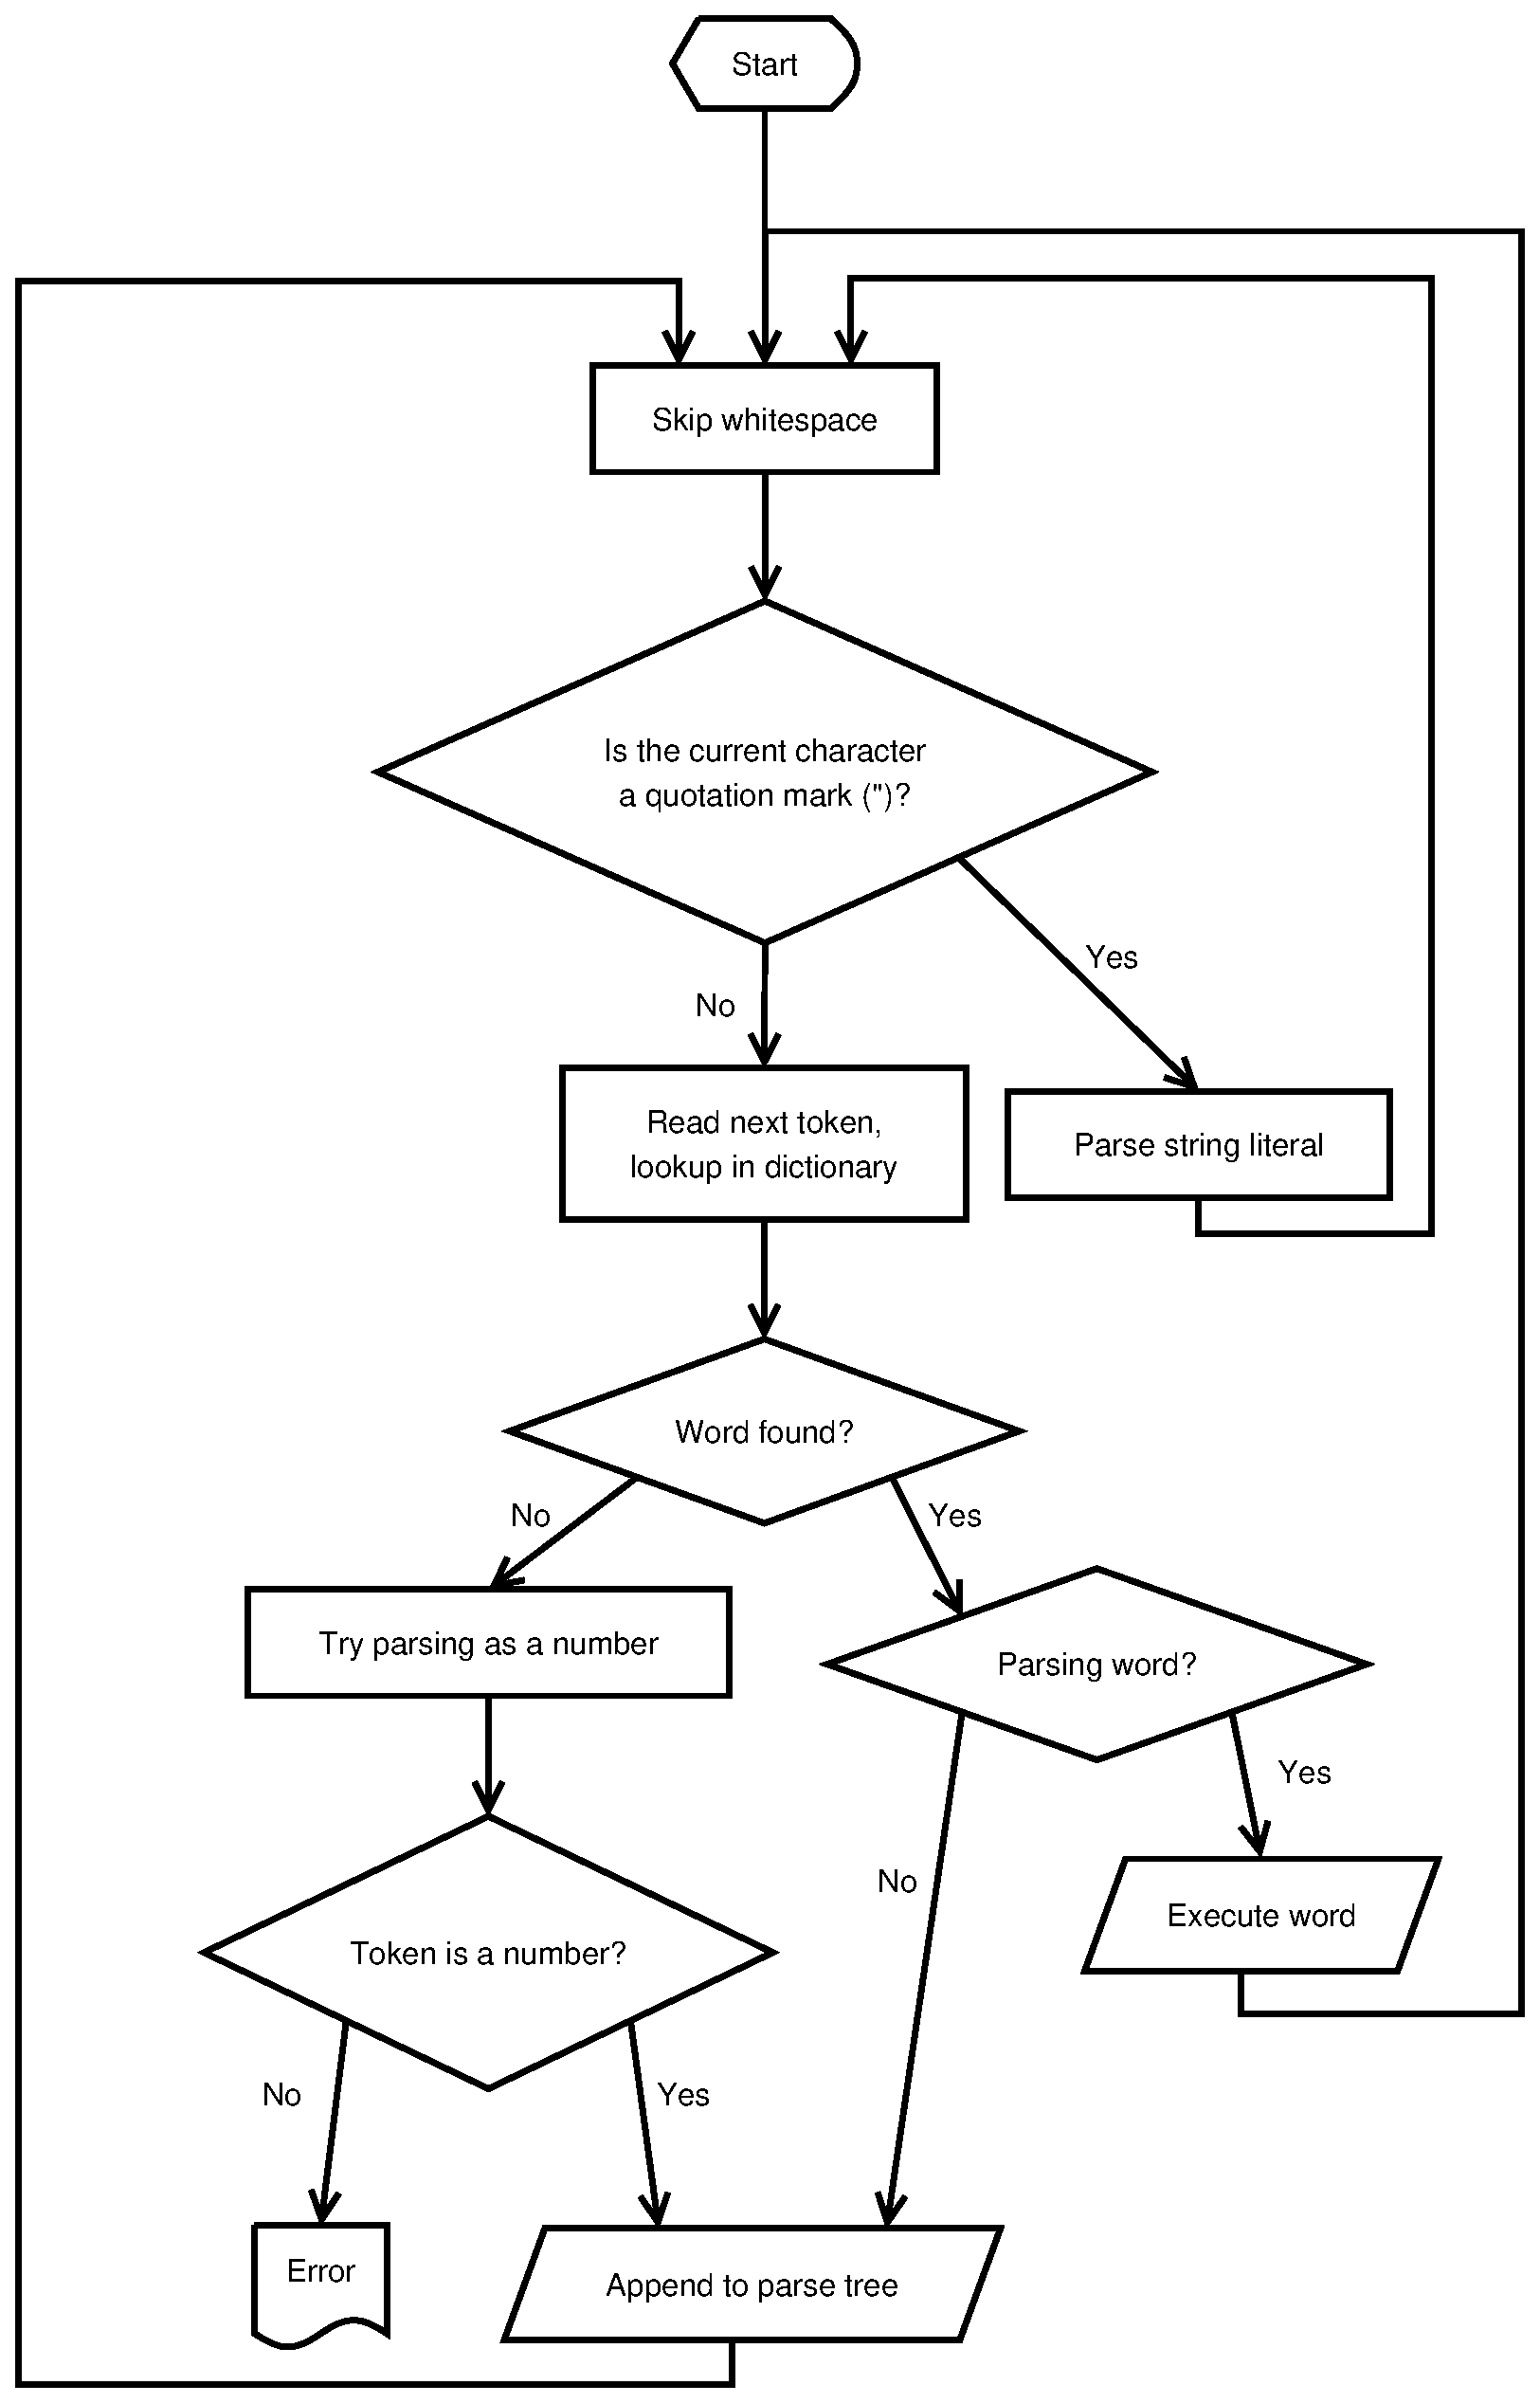
\epsfig{file=parser.eps}}
\end{center}
\end{figure}

At the most abstract level,
Factor syntax consists of whitespace-separated tokens. The parser tokenizes the input on whitespace boundaries, where whitespace is defined as a sequence or one or more space, tab, newline or carriage-return characters.  The parser is case-sensitive, so
the following three expressions tokenize differently:
\begin{verbatim}
2X+
2 X +
2 x +
\end{verbatim}
As the parser reads tokens it makes a distinction between numbers, ordinary words, and
parsing words. Tokens are appended to the parse tree, the top level of which is a list
returned by the original parser invocation. Nested levels of the parse tree are created
by parsing words.

Here is the parser algorithm in more detail -- some of the concepts therein will be defined shortly:

\begin{itemize}
\item If the current character is a double-quote (\texttt{"}), the \texttt{"} parsing word is executed, causing a string to be read.
\item Otherwise, the next token is taken from the input. The parser searches for a word named by the token in the currently used set of vocabularies. If the word is found, one of the following two actions is taken:
\begin{itemize}
\item If the word is an ordinary word, it is appended to the parse tree.
\item If the word is a parsing word, it is executed.
\end{itemize}
Otherwise if the token does not represent a known word, the parser attempts to parse it as a number. If the token is a number, the number object is added to the parse tree. Otherwise, an error is raised and parsing halts.
\end{itemize}

\glossary{name=string mode,
description={a parser mode where token strings are added to the parse tree; the parser will not look up tokens in the dictionary. Activated by switching on the \texttt{string-mode} variable}}

There is one exception to the above process; the parser might be placed in \emph{string mode}, in which case it simply reads tokens and appends them to the parse tree as strings. String mode is activated and deactivated by certain parsing words wishing to read input in an unstructured but tokenized manner -- see \ref{string-mode}.

\glossary{name=parsing word,
description={a word that is run at parse time. Parsing words can be defined by suffixing the compound definition with \texttt{parsing}. Parsing words have the \texttt{\dq{}parsing\dq{}} word property set to true, and respond with true to the \texttt{parsing?}~word}}

Parsing words play a key role in parsing; while ordinary words and numbers are simply
added to the parse tree, parsing words execute in the context of the parser, and can
do their own parsing and create nested data structures in the parse tree. Parsing words
are also able to define new words.

While parsing words supporting arbitrary syntax can be defined, the default set is found
in the \texttt{syntax} vocabulary and provides the basis for all further syntactic
interaction with Factor.

\subsection{\label{vocabsearch}Vocabulary search}

\newcommand{\wordglos}{\glossary{
name=word,
description={an object holding a code definition and set of properties. Words are organized into vocabularies, and are uniquely identified by name within a vocabulary.}}}
\wordglos
\newcommand{\vocabglos}{\glossary{
name=vocabulary,
description={a collection of words, uniquely identified by name. The hashtable of vocabularies is stored in the \texttt{vocabularies} global variable, and the \texttt{USE:}~and \texttt{USING:}~parsing words add vocabularies to the parser's search path}}}
\vocabglos

A \emph{word} associates a code definition with its name. Words are organized into \emph{vocabularies}. Vocabularies are organized into vocabularies. Words are discussed in depth in \ref{words}.

When the parser reads a token, it attempts to look up a word named by that token. The
lookup is performed in the parser's current vocabulary set. By default, this set includes
two vocabularies:
\begin{verbatim}
syntax
scratchpad
\end{verbatim}
The \texttt{syntax} vocabulary consists of a set of parsing words for reading Factor data
and defining new words. The \texttt{scratchpad} vocabulary is the default vocabulary for new
word definitions.
\wordtable{
\parsingword{USE:}{USE: \emph{vocabulary}}{syntax}
}
\newcommand{\useglos}{\glossary{
name=search path,
description={the list of vocabularies that the parser looks up tokens in. You can add to this list with the \texttt{USE:} and \texttt{USING:} parsing words}}}
\useglos

The \texttt{USE:} parsing word adds a new vocabulary at the front of the search path. Subsequent word lookups by the parser will search this vocabulary first.
\begin{alltt}
USE: lists
\end{alltt}
\wordtable{
\parsingword{USING:}{USING: \emph{vocabularies} ;}{syntax}
}
Consecutive \texttt{USE:} declarations can be merged into a single \texttt{USING:} declaration.
\begin{alltt}
USING: lists strings vectors ;
\end{alltt}

Due to the way the parser works, words cannot be referenced before they are defined; that is, source files must order definitions in a strictly bottom-up fashion. For a way around this, see \ref{deferred}.

\subsection{Numbers}

\newcommand{\numberglos}{\glossary{
name=number,
description={an instance of the \texttt{number} class}}}
\numberglos

If a vocabulary lookup of a token fails, the parser attempts to parse it as a number.

\subsubsection{Integers}

\newcommand{\integerglos}{\glossary{
name=integer,
description={an instance of the \texttt{integer} class, which is a disjoint union of the \texttt{fixnum} and \texttt{bignum} classes}}}
\numberglos

\newcommand{\fixnumglos}{\glossary{
name=fixnum,
description={an instance of the \texttt{fixnum} class, representing a fixed precision integer. On 32-bit systems, an element of the interval $(-2^{-29},2^{29}]$, and on 64-bit systems, the interval $(-2^{-61},2^{61}]$}}}
\fixnumglos

\newcommand{\bignumglos}{\glossary{
name=bignum,
description={an instance of the \texttt{bignum} class, representing an arbitrary-precision integer whose value is bounded by available object memory}}}
\bignumglos

The printed representation of an integer consists of a sequence of digits, optionally prefixed by a sign.
\begin{alltt}
123456
-10
2432902008176640000
\end{alltt}
Integers are entered in base 10 unless prefixed with a base change parsing word.
\wordtable{
\parsingword{BIN:}{BIN: \emph{integer}}{syntax}\\
\parsingword{OCT:}{OCT: \emph{integer}}{syntax}\\
\parsingword{HEX:}{HEX: \emph{integer}}{syntax}
}
\begin{alltt}
\textbf{ok} BIN: 1110 BIN: 1 + .
\textbf{15}
\textbf{ok} HEX: deadbeef 2 * .
\textbf{7471857118}
\end{alltt}

\subsubsection{Ratios}

\newcommand{\ratioglos}{\glossary{
name=ratio,
description={an instance of the \texttt{ratio} class, representing an exact ratio of two integers}}}
\ratioglos

The printed representation of a ratio is a pair of integers separated by a slash (\texttt{/}).
No intermediate whitespace is permitted. Either integer may be signed, however the ratio will be normalized into a form where the denominator is positive and the greatest common divisor
of the two terms is 1.
\begin{alltt}
75/33
1/10
-5/-6
\end{alltt}

\subsubsection{Floats}

\newcommand{\floatglos}{\glossary{
name=float,
description={an instance of the \texttt{float} class, representing an IEEE 754 double-precision floating point number}}}
\floatglos

Floating point numbers contain an optional decimal part, an optional exponent, with
an optional sign prefix on either the significand or exponent.
\begin{alltt}
10.5
-3.1456
7e13
1e-5
\end{alltt}

\subsubsection{Complex numbers}

\newcommand{\complexglos}{\glossary{
name=complex,
description={an instance of the \texttt{complex} class, representing a complex number with real and imaginary components, where both components are real numbers}}}
\complexglos
\wordtable{
\parsingword{hash-curly}{\#\{ \emph{real} \emph{imaginary} \}\#}{syntax}
}
A complex number
is given by two components, a ``real'' part and ''imaginary'' part. The components
must either be integers, ratios or floats.
\begin{verbatim}
#{ 1/2 1/3 }#   ! the complex number 1/2+1/3i
#{ 0 1 }#       ! the imaginary unit
\end{verbatim}

\subsection{Literals}

Many different types of objects can be constructed at parse time via literal syntax. Numbers are a special case since support for reading them is built-in to the parser. All other literals are constructed via parsing words.

If a quotation contains a literal object, the same literal object instance is used each time the quotation executes; that is, literals are ``live''.

\subsubsection{\label{boolean}Booleans}

\newcommand{\boolglos}{
\glossary{
name=boolean,
description={an instance of the \texttt{boolean} class, either \texttt{f} or \texttt{t}. See generalized boolean}}
\glossary{
name=generalized boolean,
description={an object used as a truth value. The \texttt{f} object is false and anything else is true. See boolean}}
\glossary{
name=t,
description={the canonical truth value. The \texttt{t} class, whose sole instance is the \texttt{t} object. Note that the \texttt{t} class is not equal to the \texttt{t} object}}
\glossary{
name=f,
description={the canonical false value; anything else is true. The \texttt{f} class, whose sole instance is the \texttt{f} object. Note that the \texttt{f} class is not equal to the \texttt{f} object}}
}
\boolglos
Any Factor object may be used as a truth value in a conditional expression. The \texttt{f} object is false and anything else is true. The \texttt{f} object is also used to represent the empty list, as well as the concept of a missing value. The canonical truth value is the \texttt{t} object.
\wordtable{
\parsingword{f}{f}{syntax}\\
\parsingword{t}{t}{syntax}
}
Adds the \texttt{f} and \texttt{t} objects to the parse tree.

Note that the \texttt{f} parsing word and class is not the same as the \texttt{f} object. The former can be obtained by writing \texttt{\bs~f} inside a quotation, or \texttt{POSTPONE: f} inside a list that will not be evaluated.
\begin{alltt}
\textbf{ok} f \bs f = .
\textbf{f}
\end{alltt}
An analogous distinction holds for the \texttt{t} class and object.

\subsubsection{\label{syntax:char}Characters}

\newcommand{\charglos}{\glossary{
name=character,
description={an integer whose value denotes a Unicode code point. Character values are limited to the range from $0$ to $2^16-1$ inclusive, however in a later release this can be upgraded to the full 21-bit Unicode space without requiring any changes to user code}}}
\charglos
Factor has no distinct character type, however Unicode character value integers can be
read by specifying a literal character, or an escaped representation thereof.
\wordtable{
\parsingword{CHAR:}{CHAR: \emph{token}}{syntax}
}
Adds the Unicode code point of the character represented by \emph{token} to the parse tree.

\newcommand{\escapeglos}{\glossary{
name=escape,
description={a sequence allowing a non-literal character to be inserted in a string. For a list of escapes, see \ref{escape}}}}
\escapeglos
If the token is a single-character string other than whitespace or backslash, the character is taken to be this token. If the token begins with a backslash, it denotes one of the following escape codes.
\begin{table}[Special character escape codes]
\label{escape}
\begin{tabular}{l|l}
Escape code&Character\\
\hline
\texttt{\bs{}\bs}&Backslash (\texttt{\bs})\\
\texttt{\bs{}s}&Space\\
\texttt{\bs{}t}&Tab\\
\texttt{\bs{}n}&Newline\\
\texttt{\bs{}t}&Carriage return\\
\texttt{\bs{}0}&Null byte (ASCII 0)\\
\texttt{\bs{}e}&Escape (ASCII 27)\\
\texttt{\bs{}"}&Double quote (\texttt{"})\\
\end{tabular}
\end{table}
Examples:
\begin{alltt}
\textbf{ok} CHAR: a .
\textbf{97}
\textbf{ok} CHAR: \bs{}0 .
\textbf{0}
\textbf{ok} CHAR: \bs{}n .
\textbf{10}
\end{alltt}
A Unicode character can be specified by its code number by writing \texttt{\bs{}u} followed by a four-digit hexadecimal. That is, the following two expressions are equivalent:
\begin{alltt}
CHAR: \bs{}u0078
78
\end{alltt}
While not useful for single characters, this syntax is also permitted inside strings.

\subsubsection{\label{string-literals}Strings}

\newcommand{\stringglos}{\glossary{
name=string,
description={an instance of the \texttt{string} class, representing an immutable sequence of characters}}}
\stringglos
\wordtable{
\parsingword{"}{"\emph{string}"}{syntax}
}
Reads from the input string until the next occurrence of
\texttt{"}, and appends the resulting string to the parse tree. String literals cannot span multiple lines.
Strings containing
the \texttt{"} character and various other special characters can be read by
inserting escape sequences as described in \ref{syntax:char}.
\begin{alltt}
\textbf{ok} "Hello world" print
\textbf{Hello world}
\end{alltt}

\subsubsection{\label{listsyntax}Lists}
\newcommand{\listglos}{\glossary{
name=list,
description={an instance of the \texttt{list} class, storing a sequence of elements as a chain of zero or more conses, where the car of each cons is an element, and the cdr is either \texttt{f} or another list}}
\glossary{name=proper list, description=see list}
}
\listglos
\wordtable{
\parsingword{openbracket}{[}{syntax}\\
\parsingword{closebracket}{]}{syntax}
}
Parses a list, whose elements are read between \texttt{[} and \texttt{]} and can include other lists.
\begin{verbatim}
[
    "404" "responder" set
    [ drop no-such-responder ] "get" set
]
\end{verbatim}
\newcommand{\consglos}{\glossary{
name=cons,
description={an instance of the \texttt{cons} class, storing an ordered pair of objects referred to as the car and the cdr}}}
\consglos
\wordtable{
\parsingword{conssyntax}{[[ \emph{car} \emph{cdr} ]]}{syntax}
}
Parses two components making up a cons cell. Note that the lists parsed with \texttt{[} and \texttt{]} are just a special case of \texttt{[[} and \texttt{]]}. The following two lines are equivalent.
\begin{alltt}
[ 1 2 3 ]
[[ 1 [[ 2 [[ 3 f ]] ]] ]]
\end{alltt}
The empty list is denoted by \texttt{f}, along with boolean falsity, and the concept of a missing value. The expression \texttt{[ ]} parses to the same object as \texttt{f}.

\subsubsection{Words}

While words parse as themselves, a word occurring inside a quotation is executed when the quotation is called. Sometimes it is desirable to have a word be pushed on the data stack during the execution of a quotation, usually for reflective access to the word's slots.
\wordtable{
\parsingword{bs}{\bs~\emph{word}}{syntax}
}
Reads the next word from the input string and appends some \emph{code} to the parse tree that pushes the word on the stack when the code is called. The following two lines are equivalent:
\begin{verbatim}
\ length
[ length ] car
\end{verbatim}
\wordtable{
\parsingword{POSTPONE:}{POSTPONE: \emph{word}}{syntax}
}
Reads the next word from the input string and appends the word to the parse tree, even if it is a parsing word. For an word \texttt{foo}, \texttt{POSTPONE: foo} and \texttt{foo} are equivalent; however, if \texttt{foo} is a parsing word, the latter will execute it at parse time, while the former will execute it at runtime. Usually used inside parsing words that wish to delegate some action to a further parsing word.
\begin{alltt}
\textbf{ok} : parsing1
    "Parsing 1" print 2 swons ; parsing
\textbf{ok} : parsing2
    "Parsing 2" print POSTPONE: parsing1 ; parsing
\textbf{ok} [ 1 parsing1 3 ] .
\textbf{Parsing 1}
\textbf{[ 1 2 3 ]}
\textbf{ok} [ 0 parsing2 2 4 ] .
\textbf{Parsing 2}
\textbf{Parsing 1}
\textbf{[ 0 2 4 ]}
\end{alltt}

\subsubsection{Mutable literals}

\newcommand{\mutableglos}{\glossary{name=mutable object,
description=an object whose slot values can be changed}
\glossary{name=immutable object,
description=an object whose slot values cannot be changed}}
\mutableglos

Using mutable object literals in word definitions requires care, since if those objects
are mutated, the actual word definition will be changed, which is in most cases not what you would expect. Strings and lists are immutable; string buffers, vectors, hashtables and tuples are mutable.

\subsubsection{\label{sbuf-literals}String buffers}

\newcommand{\sbufglos}{\glossary{
name=string buffer,
description={an instance of the \texttt{sbuf} class, representing a mutable and growable sequence of characters}}
\glossary{name=sbuf, description=see string buffer}}
\sbufglos
\wordtable{
\parsingword{SBUF}{SBUF" \emph{text}"}{syntax}
}
Reads from the input string until the next occurrence of
\texttt{"}, converts the string to a string buffer, and appends it to the parse tree.
As with strings, the escape codes described in \ref{syntax:char} are permitted.
\begin{alltt}
\textbf{ok} SBUF" Hello world" sbuf>string print
\textbf{Hello world}
\end{alltt}

\subsubsection{\label{vector-literals}Vectors}
\newcommand{\vectorglos}{\glossary{
name=vector,
description={an instance of the \texttt{vector} class, storing a mutable and growable sequence of elements in a contiguous range of memory}}}
\vectorglos
\wordtable{
\parsingword{opencurly}{\{}{syntax}\\
\parsingword{closecurly}{\}}{syntax}
}
Parses a vector, whose elements are read between \texttt{\{} and \texttt{\}}.
\begin{verbatim}
{ 3 "blind" "mice" }
\end{verbatim}

\subsubsection{Hashtables}
\newcommand{\hashglos}{\glossary{
name=hashtable,
description={an instance of the \texttt{hashtable} class, providing a mutable mapping of keys to values}}}
\hashglos
\wordtable{
\parsingword{openccurly}{\{\{}{syntax}\\
\parsingword{closeccurly}{\}\}}{syntax}
}
Parses a hashtable. Elements between \texttt{\{\{} and \texttt{\}\}} must be cons cells, where the car is the key and the cdr is a value.
\begin{verbatim}
{{
    [[ "red" [ 255 0 0 ] ]]
    [[ "green" [ 0 255 0 ] ]]
    [[ "blue" [ 0 0 255 ] ]]
}}
\end{verbatim}

\subsubsection{Tuples}
\newcommand{\tupleglos}{\glossary{
name=tuple,
description={an instance of a user-defined class whose metaclass is the \texttt{tuple} metaclass, storing a fixed set of elements in named slots, with optional delegation method dispatch semantics}}}
\tupleglos
\wordtable{
\parsingword{<<}{<<}{syntax}\\
\parsingword{>>}{>>}{syntax}
}
Parses a tuple. The tuple's class must follow \texttt{<<}. The element after that is always the tuple's delegate. Further elements until \texttt{>>} are specified according to the tuple's slot definition, and an error is raised if an incorrect number of elements is given.
\begin{verbatim}
<< color f 255 0 0 >>
\end{verbatim}

\subsection{\label{comments}Comments}

\wordtable{
\parsingword{!}{!~\emph{remainder of line}}{syntax}
}
The remainder of the input line is ignored if an exclamation mark (\texttt{!}) is read.
\begin{alltt}
! Note that the sequence union does not include lists,
! or user defined tuples that respond to the sequence
! protocol.
\end{alltt}
\wordtable{
\parsingword{hash!}{\#!~\emph{remainder of line}}{syntax}
}
\newcommand{\doccommentglos}{\glossary{
name=documentation comment,
description={a comment describing the usage of a word. Delimited by the \texttt{\#"!} parsing word, they appear at the start of a word definition and are stored in the \texttt{""documentation""} word property}}}
\doccommentglos
Comments that begin with \texttt{\#!} are called \emph{documentation comments}.
A documentation comment has no effect on the generated parse tree, but if it is the first thing inside a word definition, the comment text is appended to the string stored in the word's \texttt{"documentation"} property. Word properties are described in \ref{word-props}.
\wordtable{
\parsingword{(}{( \emph{stack effect} )}{syntax}
}
\glossary{
name=stack effect,
description={A string of the form \texttt{( \emph{inputs} -- \emph{outputs} )}, where the inputs and outputs are a whitespace-separated list of names or types. The top of the stack is the right-most token on both sides.}}
\newcommand{\stackcommentglos}{\glossary{
name=stack effect comment,
description={a comment describing the inputs and outputs of a word. Delimited by \texttt{(} and \texttt{}), they appear at the start of a word definition and are stored in the \texttt{""stack-effect""} word property}}}
\stackcommentglos
Comments delimited by \texttt{(} and \texttt{)} are called \emph{stack effect comments}. By convention they are placed at the beginning of a word definition to document the word's inputs and outputs:
\begin{verbatim}
: push ( element sequence -- )
    #! Push a value on the end of a sequence.
    dup length swap set-nth ;
\end{verbatim}
A stack effect comment has no effect on the generated parse tree, but if it is the first thing inside a word definition, the word's \texttt{"stack-effect"} property is set to the comment text. Word properties are described in \ref{word-props}.

\section{Data and control flow}

\subsection{Shuffle words}

\newcommand{\dsglos}{\glossary{
name=stack,
description=see data stack}
\glossary{
name=data stack,
description={the primary means of passing values between words}}}
\dsglos
Shuffle words are placed between words taking action to rearrange items on the stack
as the next word in the quotation would expect them. Their behavior can be understood entirely in terms of their stack effects.
\wordtable{
\ordinaryword{drop}{drop ( x -- )}{kernel}\\
\ordinaryword{2drop}{drop ( x y -- )}{kernel}\\
\ordinaryword{3drop}{drop ( x y z -- )}{kernel}\\
\ordinaryword{nip}{nip ( x y -- y )}{kernel}\\
\ordinaryword{2nip}{2nip ( x y -- y )}{kernel}\\
\ordinaryword{dup}{dup ( x -- x x )}{kernel}\\
\ordinaryword{2dup}{2dup ( x y -- x y x y )}{kernel}\\
\ordinaryword{3dup}{3dup ( x y z -- x y z x y z )}{kernel}\\
\ordinaryword{dupd}{dupd ( x y -- x x y )}{kernel}\\
\ordinaryword{over}{over ( x y -- x y x )}{kernel}\\
\ordinaryword{pick}{pick ( x y z -- x y z x )}{kernel}\\
\ordinaryword{tuck}{tuck ( x y -- y x y )}{kernel}\\
\ordinaryword{swap}{swap ( x y -- y x )}{kernel}\\
\ordinaryword{2swap}{2swap ( x y z t -- z t x y )}{kernel}\\
\ordinaryword{swapd}{swapd ( x y z -- y x z )}{kernel}\\
\ordinaryword{rot}{rot ( x y z -- y z x )}{kernel}\\
\ordinaryword{-rot}{-rot ( x y z -- z x y )}{kernel}
}
Try to avoid the complex shuffle words such as \texttt{rot} and \texttt{2dup} as much as possible, for they make data flow harder to understand. If you find yourself using too many shuffle words, or you're writing
a stack effect comment in the middle of a compound definition to keep track of stack contents, it is
a good sign that the word should probably be factored into two or
more smaller words.

\subsection{\label{quotations}Quotations}

\newcommand{\csglos}{\glossary{
name=return stack,
description=see call stack}
\glossary{
name=call stack,
description={holds quotations waiting to be called. When a quotation is called with \texttt{call}, or when a compound word is executed, the previous call frame is pushed on the call stack, and the new quotation becomes the current call frame}}}
\csglos
\newcommand{\cfglos}{\glossary{
name=call frame,
description=the currently executing quotation}}
\cfglos
\glossary{
name=interpreter,
description=executes quotations by iterating them and recursing into nested definitions. see compiler}

\begin{figure}
\begin{center}
\caption{Interpreter algorithm}
\scalebox{0.45}{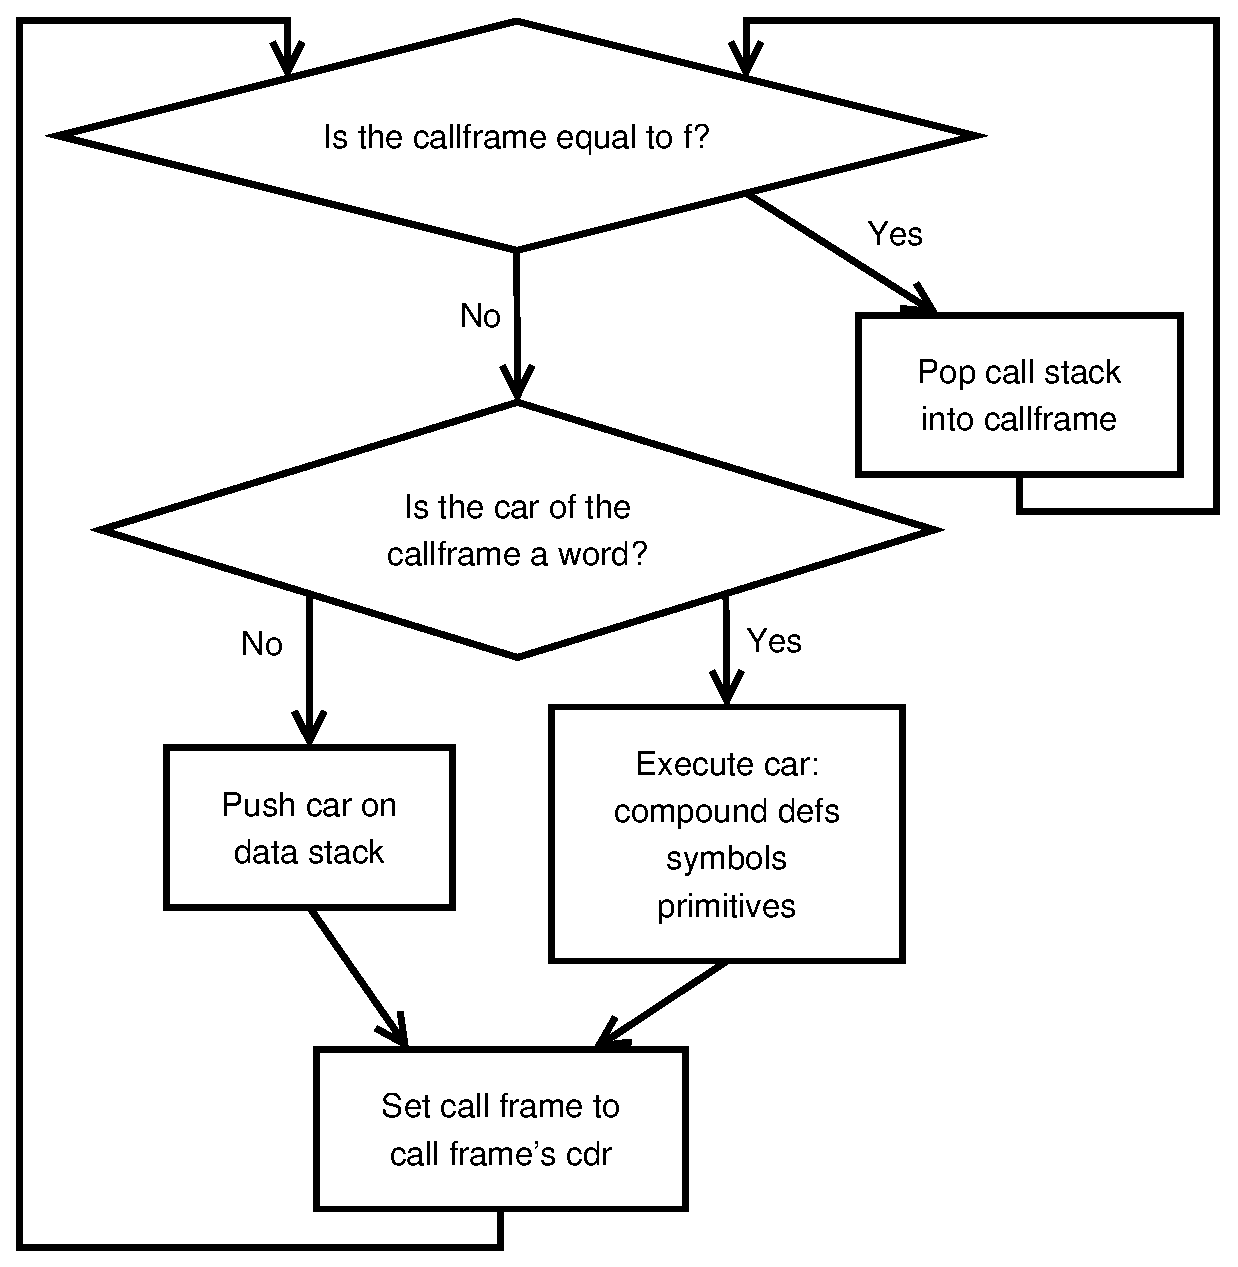
\epsfig{file=interpreter.eps}}
\end{center}
\end{figure}

The Factor interpreter executes quotations. Quotations are lists, and since lists can contain any Factor object, they can contain words. It is words that give quotations their operational behavior, as you can see in the following description of the interpreter algorithm.

\begin{itemize}
\item If the call frame is \texttt{f}, the call stack is popped and becomes the new call frame.
\item If the car of the call frame is a word, the word is executed:
\begin{itemize}
\item If the word is a symbol, it is pushed on the data stack. See \ref{symbols}.
\item If the word is a compound definition, the current call frame is pushed on the call stack, and the new call frame becomes the word definition. See \ref{colondefs}.
\item If the word is compiled or primitive, the interpreter jumps to a machine code definition. See \ref{primitives}.
\item If the word is undefined, an error is raised. See \ref{deferred}.
\end{itemize}
\item Otherwise, the car of the call frame is pushed on the data stack.
\item The call frame is set to the cdr, and the loop continues.
\end{itemize}

The interpreter can be invoked reflectively with the following pair of words.
\wordtable{
\ordinaryword{call}{call ( quot -- )}{kernel}
}
Push the current call frame on the call stack, and set the call stack to the given quotation. Conceptually: calls the quotation, as if its definition was substituted at the location of the \texttt{call}.
\begin{alltt}
\textbf{ok} [ 2 2 + 3 * ] call .
\textbf{12}
\end{alltt}
\wordtable{
\ordinaryword{execute}{execute ( word -- )}{kernel}
}
Execute a word definition, taking action based on the word definition, as above.
\begin{alltt}
\textbf{ok} : hello "Hello world" print ;
\textbf{ok} : twice dup execute execute ;
\textbf{ok} \bs hello twice
\textbf{Hello world}
\textbf{Hello world}
\end{alltt}

\subsubsection{Tail call optimization}

\newcommand{\tailglos}{\glossary{
name=tail call,
description=the last call in a quotation}
\glossary{
name=tail call optimization,
description=the elimination of call stack pushes when making a tail call}}

When a call is made to a quotation from the last word in the call frame, there is no
purpose in pushing the empty call frame on the call stack. Therefore the last call in a quotation does not grow the call stack, and tail recursion executes in bounded space.

\subsubsection{Call stack manipulation}

Because of the way the interpreter is described in \ref{quotations}, the top of the call stack is not accessed during the execution of a quotation; it is only popped when the interpreter reaches the end of the quotation. In effect, the call stack can be used as a temporary storage area, as long as pushes and pops are balanced out within a single quotation.
\wordtable{
\ordinaryword{>r}{>r ( x -- r:x )}{kernel}
}
Moves the top of the data stack to the call stack.
\wordtable{
\ordinaryword{r>}{r> ( x -- r:x )}{kernel}
}
Moves the top of the call stack to the data stack.

The top of the data stack is ``hidden'' between \texttt{>r} and \texttt{r>}.
\begin{alltt}
\textbf{ok} 1 2 3 >r .s r>
\textbf{2
1}
\end{alltt}
It is very important to balance usages of \texttt{>r} and \texttt{r>} within a single quotation or word definition.
\begin{verbatim}
: the-good >r 2 + r> * ; ! Okay
: the-bad  >r 2 + ;      ! Runtime error
: the-ugly r> ;          ! Runtime error
\end{verbatim}
Basically, the rule is you must leave the call stack in the same state as you found it, so that when the current quotation finishes executing, the interpreter can return to the caller.

One exception is that when \texttt{ifte} occurs as the last word in a definition, values may be pushed on the call stack before the condition value is computed, as long as both branches of the \texttt{ifte} pop the values off the call stack before returning.
\begin{verbatim}
: foo ( m ? n -- m+n/n )
    >r [ r> + ] [ drop r> ] ifte ; ! Okay
\end{verbatim}

\subsubsection{Quotation variants}

There are three words that combine shuffle words with \texttt{call}. They are useful in the implementation of higher-order words taking quotations as inputs.
\wordtable{
\ordinaryword{slip}{slip ( quot x -- x | quot: -- )}{kernel}
}
Call a quotation, while hiding the top of the stack. The implementation is as you would expect.
\begin{verbatim}
: slip ( quot x -- x | quot: -- )
    >r call r> ; inline
\end{verbatim}
\wordtable{
\ordinaryword{keep}{keep ( x quot -- x | quot:~x -- )}{kernel}
}
Call a quotation with a value on the stack, restoring the value when the quotation returns.
\begin{verbatim}
: keep ( x quot -- x | quot: x -- )
    over >r call r> ; inline
\end{verbatim}
\wordtable{
\ordinaryword{2keep}{2keep ( x y q -- x y | q:~x y -- )}{kernel}
}
Call a quotation with a pair of values on the stack, restoring the values when the quotation returns.
\begin{verbatim}
: 2keep ( x y quot -- x y | quot: x y -- )
    over >r pick >r call r> r> ; inline
\end{verbatim}

\subsection{Conditionals}

The simplest style of a conditional form is the \texttt{ifte} word.
\wordtable{
\ordinaryword{ifte}{ifte ( cond true false -- )}{kernel}
}
The \texttt{cond} is a generalized boolean. If it is \texttt{f}, the \texttt{false} quotation is called, and if \texttt{cond} is any other value, the \texttt{true} quotation is called. The condition flag is removed from the stack before either quotation executes.

Note that in general, both branches should have the same stack effect. Not only is this good style that makes the word easier to understand, but also unbalanced conditionals cannot be compiled.
\wordtable{
\ordinaryword{when}{when ( cond true -- | true:~-- )}{kernel}\\
\ordinaryword{unless}{unless ( cond false -- | false:~-- )}{kernel}
}
This pair are minor variations on \texttt{ifte} where only one branch is specified. The other is implicitly \texttt{[ ]}. They are implemented in the trivial way:
\begin{verbatim}
: when [ ] ifte ; inline
: unless [ ] swap ifte ; inline
\end{verbatim}
The \texttt{ifte} word removes the condition flag from the stack before calling either quotation. Sometimes this is not desirable, if the condition flag is serving a dual purpose as a value to be consumed by the \texttt{true} quotation. The \texttt{ifte*} word exists for this purpose.
\wordtable{
\ordinaryword{ifte*}{ifte*~( cond true false -- )}{kernel}\\
\texttt{true:~cond --}\\
\texttt{false:~--}
}
If the condition is true, it is retained on the stack before the \texttt{true} quotation is called. Otherwise, the condition is removed from the stack and the \texttt{false} quotation is called. The following two lines are equivalent:
\begin{verbatim}
X [ Y ] [ Z ] ifte*
X dup [ Y ] [ drop Z ] ifte
\end{verbatim}
\wordtable{
\ordinaryword{when*}{when*~( cond true -- | true:~cond -- )}{kernel}\\
\ordinaryword{unless*}{unless*~( cond false -- | false:~-- )}{kernel}
}
These are variations of \texttt{ifte*} where one of the quotations is \texttt{[ ]}.

There is one final conditional form that is used to implement the ``default value'' idiom.
\wordtable{
\ordinaryword{?ifte}{?ifte ( default cond true false -- )}{kernel}\\
\texttt{true:~cond --}\\
\texttt{false:~default --}
}
If the condition is \texttt{f}, the \texttt{false} quotation is called with the \texttt{default} value on the stack. Otherwise, the \texttt{true} quotation is called with the condition on the stack. The following two lines are equivalent:
\begin{verbatim}
X [ Y ] [ Z ] ?ifte
X dup [ nip Y ] [ drop Z ] ifte
\end{verbatim}

\subsubsection{Boolean logic}

The \texttt{?}~word chooses between two values, rather than two quotations.
\wordtable{
\ordinaryword{?}{?~( cond true false -- true/false )}{kernel}
}
It is implemented in the obvious way.
\begin{verbatim}
: ? ( cond t f -- t/f )
    rot [ drop ] [ nip ] ifte ; inline
\end{verbatim}
Several words use \texttt{?}~to implement typical boolean algebraic operations.
\wordtable{
\ordinaryword{>boolean}{>boolean ( obj -- t/f )}{kernel}
}
Convert a generalized boolean into a boolean. That is, \texttt{f} retains its value, whereas anything else becomes \texttt{t}.
\wordtable{
\ordinaryword{not}{not ( ?~-- ?~)}{kernel}
}
Given \texttt{f}, outputs \texttt{t}, and on any other input, outputs \texttt{f}.
\wordtable{
\ordinaryword{and}{and ( ?~?~-- ?~)}{kernel}
}
Outputs \texttt{t} if both of the inputs are true.
\wordtable{
\ordinaryword{or}{or ( ?~?~-- ?~)}{kernel}
}
Outputs \texttt{t} if at least one of the inputs is true.
\wordtable{
\ordinaryword{xor}{xor ( ?~?~-- ?~)}{kernel}
}
Outputs \texttt{t} if exactly one of the inputs is true.
\wordtable{
\ordinaryword{implies}{implies ( b1~b2~-- ?~)}{kernel}
}
Outputs \texttt{t} if \texttt{b1} is false or both inputs are true.

An alternative set of logical operations operate on individual bits of integers bitwise, rather than generalized boolean truth values. They are documented in \ref{bitwise}.

\subsection{Continuations}

\newcommand{\contglos}{
\glossary{name=continuation,
description=an object representing the future of the computation}}
\contglos
At any point in the execution of a Factor program, the \emph{current continuation} represents the future of the computation. This object can be captured with the \texttt{callcc0} and \texttt{callcc1} words.
\wordtable{
\ordinaryword{callcc0}{callcc0 ( quot -- )}{kernel}\\
\texttt{quot:~cont --}\\
\texttt{cont:~--}\\
\ordinaryword{callcc1}{callcc1 ( quot -- )}{kernel}\\
\texttt{quot:~cont --}\\
\texttt{cont:~obj --}
}
Calling one of these words calls the given quotation with the continuation on the stack. The continuation is itself a quotation, and calling it \emph{continues execution} at the point after the call to \texttt{callcc0} and \texttt{callcc1}. Essentially, a continuation is a snapshot of the four stacks that can be restored at a later time.

The difference between \texttt{callcc0} and \texttt{callcc1} lies in the continuation object. When \texttt{callcc1} is used, calling the continuation takes one value from the top of the data stack, and places it back on the \emph{restored} data stack. This allows idioms such as exception handling, co-routines and generators to be implemented via continuations.

\subsubsection{\label{exceptions}Handling exceptional situations}
\glossary{name=exception,
description=an object representing an exceptional situation that has been detected}

Support for handling exceptional situations such as bad user input, implementation bugs, and input/output errors is provided by a pair of words, \texttt{throw} and \texttt{catch}.
\wordtable{
\ordinaryword{throw}{throw ( exception -- )}{errors}
}
Raises an exception. Execution does not continue at the point after the \texttt{throw} call. Rather, the innermost catch block is invoked, and execution continues at that point. Passing \texttt{f} as an exception will cause \texttt{throw} to do nothing.
\wordtable{
\ordinaryword{catch}{catch ( try handler -- )}{errors}\\
\texttt{handler:~exception/f -- }
}
An exception handler is established, and the \texttt{try} quotation is called.

If the \texttt{try} quotation throws an error and no nested \texttt{catch} is established, the following sequence of events takes place:
\begin{itemize}
\item the stacks are restored to their state prior to the \texttt{catch} call,
\item the exception is pushed on the data stack,
\item the \texttt{handler} quotation is called.
\end{itemize}
If the \texttt{try} quotation completes successfully, the stacks are \emph{not} restored. The \texttt{f} object is pushed, and the \texttt{handler} quotation is called.

A common idiom is that the \texttt{catch} block cleans up from the error in some fashion, then passes it on to the next-innermost catch block. The following word is used for this purpose.
\wordtable{
\ordinaryword{rethrow}{throw ( exception -- )}{errors}
}
Raises an exception, without saving the current stacks for post-mortem inspection. This is done so that inspecting the error stacks sheds light on the original cause of the exception, rather than the point where it was rethrown.

Here is a simple example of a word definition that attempts to convert a string representing a hexadecimal number into an integer, and instead of halting execution when the string is not valid, it simply outputs \texttt{f}.
\begin{verbatim}
: catch-hex> ( str -- n/f )
    [ hex> ] [ [ drop f ] when ] catch ;
\end{verbatim}
Exception handling is implemented using a \emph{catch stack}. The \texttt{catch} word pushes the current continuation on the catch stack, and \texttt{throw} calls the continuation at the top of the catch stack with the raised exception.
\glossary{name=catch stack,
description={a stack of exception handler continuations, pushed and popped by \texttt{catch}}}

\subsubsection{Multitasking}

Factor implements co-operative multitasking, where the thread of control switches between tasks at explicit calls to \texttt{yield}, as well as when blocking I/O is performed. Multitasking is implemented via continuations.
\wordtable{
\ordinaryword{in-thread}{in-thread ( quot -- )}{threads}
}
Calls \texttt{quot} in a co-operative thread. The new thread begins executing immediately, and the current thread resumes when the quotation yields, either from blocking
I/O or an explicit call to \texttt{yield}. This is implemented by adding the current continuation to the run queue, then calling \texttt{quot}, and finally executing \texttt{stop} after \texttt{quot} returns.
\wordtable{
\ordinaryword{yield}{yield ( -- )}{threads}
}
Add the current continuation to the end of the run queue, and call the continuation at the front of the run queue.
\wordtable{
\ordinaryword{stop}{stop ( -- )}{threads}
}
Call the continuation at the front of run queue, without saving the current continuation. In effect, this stops the current thread.

\subsubsection{Interpreter state}

The current state of the interpreter is determined by the contents of the four stacks. A set of words for getting and setting stack contents are the primitive building blocks for continuations, and in turn abstractions such as exception handling and multitasking.
\wordtable{
\ordinaryword{datastack}{datastack ( -- vector )}{kernel}\\
\ordinaryword{set-datastack}{set-datastack ( vector -- )}{kernel}
}
Save and restore the data stack contents. As an example, here is a word that executes a quotation and restores the data stack to its previous state;
\begin{verbatim}
: keep-datastack
    ( quot -- ) datastack slip set-datastack drop ;
\end{verbatim}
Note that the \texttt{drop} call is made to remove the original quotation from the stack.
\wordtable{
\ordinaryword{callstack}{callstack ( -- vector )}{kernel}\\
\ordinaryword{set-callstack}{set-callstack ( vector -- )}{kernel}
}
Save and restore the call stack contents. The call stack does not include the currently executing quotation that made the call to \texttt{callstack}, since the current quotation is held in the call frame -- \ref{quotations} has details. Similarly, calling \texttt{set-callstack} will continue executing the current quotation until it returns, at which point control transfers to the quotation at the top of the new call stack.
\wordtable{
\ordinaryword{namestack}{namestack ( -- list )}{namespaces}\\
\ordinaryword{set-namestack}{set-namestack ( list -- )}{namespaces}
}
Save and restore the name stack, used for dynamic variable bindings. See \ref{namespaces}.
\wordtable{
\ordinaryword{catchstack}{catchstack ( -- list )}{errors}\\
\ordinaryword{set-catchstack}{set-catchstack ( list -- )}{errors}
}
Save and restore the catch stack, used for exception handling. See \ref{exceptions}.

\section{\label{words}Words}

\wordglos
\vocabglos
\glossary{name=defining word,
description=a word that adds definitions to the dictionary}
\glossary{name=dictionary,
description=the collection of vocabularies making up the code in the Factor image}
Words are the fundamental unit of code in Factor, analogous to functions or procedures in other languages. Words are also objects, and this concept forms the basis for Factor's meta-programming facilities. Words hold two distinct pieces of information:
\begin{itemize}
\item A definition, specifying the behavior of the word when executed,
\item A set of word properties, including the name of the word, its vocabulary, any documentation strings, and other meta-data.
\end{itemize}
\wordtable{
\ordinaryword{word?}{word?~( object -- ?~)}{words}
}
Tests if the \texttt{object} is a word.
\wordtable{
\classword{word}{words}
}
The class of words.

\subsection{Vocabularies}
\wordtable{
\symbolword{vocabularies}{words}
}
Words are organized into named vocabularies, stored in the global \texttt{vocabularies} variable.
\wordtable{
\parsingword{IN:}{IN:~\emph{vocabulary}}{syntax}
}
Sets the current vocabulary for new word definitions, and adds the vocabulary to the search path (\ref{vocabsearch}).

Parsing words add definitions to the current vocabulary. When a source file is being parsed, the current vocabulary is initially set to \texttt{scratchpad}.

\subsubsection{Searching for words}

Words whose names are known at parse time -- that is, most words making up your program -- can be referenced by stating their name. However, the parser itself, and sometimes code you write, will need to look up words dynamically.
\wordtable{
\ordinaryword{search}{search ( name vocabs -- word )}{words}
}
The \texttt{vocabs} parameter is a list of vocabulary names. If a word with the given name is found, it is pushed on the stack, otherwise, \texttt{f} is pushed.

\subsubsection{Creating words}

\wordtable{
\ordinaryword{create}{create ( name vocabulary -- word )}{words}
}
Creates a new word \texttt{name} in \texttt{vocabulary}. If the vocabulary already contains a word with this name, the existing word is returned.
\wordtable{
\ordinaryword{create-in}{create-in ( name -- word )}{words}
}
Creates a new word \texttt{name} in the current vocabulary. Should only be called from parsing words (\ref{parsing-words}), and in fact is defined as:
\begin{verbatim}
: create-in ( name -- word ) "in" get create ;
\end{verbatim}

\subsection{Word definition}

There are two ways to create a word definition:
\begin{itemize}
\item Using parsing words at parse time,
\item Using defining words at run-time. This is a more dynamic feature that can be used to implement code generation and such, and in fact parse-time defining words are implemented in terms of run-time defining words.
\end{itemize}

\subsubsection{\label{colondefs}Compound definitions}

\newcommand{\colonglos}{\glossary{
name=compound definition,
description=a word defined to execute a quotation consisting of existing words}
\glossary{
name=colon definition,
description=see compound definition}}
\colonglos
A compound definition associates a word name with a quotation that is called when the word is executed.
\wordtable{
\parsingword{:}{:~\emph{name} \emph{definition} ;}{syntax}
}
A word \texttt{name} is created in the current vocabulary, and is associated with \texttt{definition}.
\begin{verbatim}
: ask-name ( -- name )
    "What is your name? " write read-line ;
: greet ( name -- )
    "Greetings, " write print ;
: friend ( -- )
    ask-name greet ;
\end{verbatim}
By convention, the word name should be followed by a stack effect comment, and for more complex definitions, a documentation comment; see \ref{comments}.
\wordtable{
\ordinaryword{define-compound}{define-compound ( word quotation -- )}{words}
}
Defines \texttt{word} to call the \texttt{quotation} when executed.
\wordtable{
\ordinaryword{compound?}{compound?~( object -- ?~)}{words}
}
Tests if the \texttt{object} is a compound word definition.
\wordtable{
\classword{compound}{words}
}
The class that all compound words are an instance of.

\subsubsection{\label{symbols}Symbols}

\newcommand{\symbolglos}{\glossary{
name=symbol,
description={a word defined to push itself on the stack when executed, created by the \texttt{SYMBOL:}~parsing word}}}
\symbolglos
\wordtable{
\parsingword{SYMBOL:}{SYMBOL:~\emph{name}}{syntax}
}
A word \texttt{name} is created in the current vocabulary that pushes itself on the stack when executed. Symbols are used to identify variables (\ref{namespaces}) as well as for storing crufties in their properties (\ref{word-props}).
\wordtable{
\ordinaryword{define-symbol}{define-symbol ( word -- )}{words}
}
Defines \texttt{word} to push itself on the data stack when executed.
\wordtable{
\ordinaryword{symbol?}{symbol?~( object -- ?~)}{words}
}
Tests if the \texttt{object} is a symbol.
\wordtable{
\classword{symbol}{words}
}
The class that all symbols are an instance of.

\subsubsection{\label{primitives}Primitives}
\newcommand{\primglos}{\glossary{
name=primitive,
description=a word implemented as native code in the Factor runtime}}
\symbolglos

Executing a primitive invokes native code in the Factor runtime. Primitives cannot be defined through Factor code. Compiled definitions behave similarly to primitives in that the interpreter jumps to native code upon encountering them.
\wordtable{
\ordinaryword{primitive?}{primitive?~( object -- ?~)}{words}
}
Tests if the \texttt{object} is a primitive.
\wordtable{
\classword{primitive}{words}
}
The class that all primitives are an instance of.

\subsubsection{\label{deferred}Deferred words and mutual recursion}

\glossary{
name=deferred word,
description={a word without a definition, created by the \texttt{DEFER:}~parsing word}}
Due to the way the parser works, words cannot be referenced before they are defined; that is, source files must order definitions in a strictly bottom-up fashion. Mutually-recursive pairs of words can be implemented by \emph{deferring} one of the words in the pair so that the second word in the pair can parse, then by replacing the deferred definition with a real one.
A demonstration of the idiom:
\begin{verbatim}
DEFER: foe
: fie ... foe ... ;
: foe ... fie ... ;
\end{verbatim}
\wordtable{
\parsingword{DEFER:}{DEFER:~\emph{name}}{syntax}
}
Create a word \texttt{name} in the current vocabulary that simply raises an error when executed. Usually, the word will be replaced with a real definition later.
\wordtable{
\ordinaryword{undefined?}{undefined?~( object -- ?~)}{words}
}
Tests if the \texttt{object} is an undefined (deferred) word.
\wordtable{
\classword{undefined}{words}
}
The class that all undefined words are an instance of.

\subsubsection{Undefining words}

\wordtable{
\parsingword{FORGET:}{FORGET:~\emph{name}}{syntax}
}
Removes the word \texttt{name} from its vocabulary. Existing definitions that reference the word will continue to work, but newly-parsed occurrences of the word will not locate the forgotten definition. No exception is thrown if no such word exists.
\wordtable{
\ordinaryword{forget}{forget ( word -- )}{words}
}
Removes the word from its vocabulary. The parsing word \texttt{FORGET:} is implemented using this word.

\subsection{\label{word-props}Word properties}

\glossary{name=word property,
description={a name/value pair stored in a word's properties}}
\glossary{name=word properties,
description={a hashtable associated with each word storing various sundry properties}}

Each word has an associated hashtable of properties. Conventionally, the property names are strings, but nothing requires that this be so.

A common idiom in the Factor library is to use symbols for their properties. 

\wordtable{
\ordinaryword{word-prop}{word-prop ( word name -- value )}{words}\\
\ordinaryword{set-word-prop}{set-word-prop ( value word name -- )}{words}
}
Retrieve and store word properties. Note that the stack effect is designed so that it is most convenient when \texttt{name} is a literal that is pushed on the stack right before executing these words. This is usually the case.

\wordtable{
\ordinaryword{word-name}{word-prop ( word -- name )}{words}\\
\ordinaryword{word-vocabulary}{word-vocabulary ( word -- vocabulary )}{words}
}
Retreive the name of a word, and the name of the vocabulary it is stored in. The definitions are trivial:
\begin{verbatim}
: word-name "name" word-prop ;
: word-vocabulary "vocabulary" word-prop ;
\end{verbatim}

\wordtable{
\ordinaryword{word-sort}{word-sort ( list -- list )}{words}
}
Sort a list of words by name.

\wordtable{
\ordinaryword{word-props}{word-props ( word -- hashtable )}{words}\\
\ordinaryword{set-word-props}{set-word-props ( hashtable word -- )}{words}
}
Retreive and store the entire set of word properties.

\subsection{Low-level details}

The actual behavior of a word when executed is determined by the values of two slots:
\begin{itemize}
\item The primitive number
\item The primitive parameter
\end{itemize}
The primitive number is an index into an array of native functions in the Factor runtime.
Some frequently-occurring primitive numbers:
\begin{description}
\item[0] deferred word,
\item[1] compound definition -- executes the quotation stored in the parameter slot,
\item[2] symbol -- pushes the value of the parameter slot,
\item[3 onwards] the actual set of primitives, of which there are around 170.
\end{description}
The words outlined in this section should not be used in ordinary code.
\wordtable{
\ordinaryword{word-primitive}{word-primitive ( word -- n )}{words}\\
\ordinaryword{set-word-primitive}{set-word-primitive ( word -- n )}{words}
}
Retrieves and stores a word's primitive number.

\wordtable{
\ordinaryword{word-def}{word-def ( word -- object )}{words}\\
\ordinaryword{set-word-def}{set-word-def ( object word -- )}{words}
}
Retrieves and stores a word's primitive parameter. This parameter is only used if the primitive number is 1 (compound definitions) or 2 (symbols). Note that to define a compound definition or symbol, you must use \texttt{define-compound} or \texttt{define-symbol}, as these words do not update the cross-referencing of word dependencies.

\wordtable{
\ordinaryword{word-xt}{word-xt ( word -- n )}{words}\\
\ordinaryword{set-word-xt}{set-word-xt ( n word -- )}{words}
}
Retrieves and stores a word's \emph{execution token}.

This is an even lower-level facility for working with the address containing native code to be invoked when the word is executed. The compiler sets the execution token to a location in memory containing generated code.

\wordtable{
\ordinaryword{update-xt}{update-xt ( word -- )}{words}
}
Updates a word's execution token according to its primitive number. When called with a compiled word, has the effect of decompiling the word. The execution token is automatically updated after a call to \texttt{set-word-primitive}.

\wordtable{
\ordinaryword{recrossref}{recrossref ( word -- )}{words}
}
Updates the cross-referencing database, which you will probably need to do if you mess around with any of the words in this section -- assuming Factor does not crash first, that is.

\chapter{The library}

\section{Objects}

\glossary{name=object,
description=a datum that can be identified}
\mutableglos

Everything in Factor is an object, where an object is a collection of slots. Each object has a unique identity, and references to objects are passed by value on the stack. It is possible to have two references to the same object, and if the object is mutated through one reference, the changes will be visible through the other reference. Not all objects are mutable; the documentation for each class details if its instances are mutable or not.

\subsection{\label{equality}Identity and equality}

\glossary{name=equal,
description={two objects are equal if they have the same class and if their slots are equal, or alternatively, if both are numbers that denote the same value}}
There are two distinct notions of ``sameness'' when it comes to objects. You can test if two references point to the same object, or you can test if two objects are equal in some sense, usually by having the same type and equal slot values.
\wordtable{
\ordinaryword{eq?}{eq?~( object object -- ?~)}{kernel}
}
Output \texttt{t} if two references point to the same object, and \texttt{f} otherwise.
\wordtable{
\genericword{=}{= ( object object -- ?~)}{kernel}
}
Output \texttt{t} if two objects are equal, and \texttt{f} otherwise. The precise meaning of equality depends on the object's class, however usually two objects are equal if their slot values are equal. If two objects are equal, they have the same printed representation, although the converse is not always true. In particular:
\begin{itemize}
\item If no more specific method is defined, \texttt{=} calls \texttt{eq?}.
\item Two numbers are equal if they have the same numerical value.
\item Two sequences are equal if they are both instances of the same class, and if they have the same length, and elements.
\item Two hashtables are equal if they hold the same set of key/value pairs.
\item Two tuples are equal if they are of the same class and their slots are equal.
\item Two words are equal if they are the same object.
\end{itemize}
\wordtable{
\genericword{clone}{clone ( object -- object )}{kernel}
}
Make a fresh object that is equal to the given object. This is not guaranteed to actually copy the object; it does nothing with immutable objects, and does not copy words either. However, sequences and tuples can be cloned to obtain a new shallow copy of the original.

\subsection{Generic words and methods}

\glossary{name=generic word,
description={a word defined using the \texttt{GENERIC:}~parsing word. The behavior of generic words depends on the class of the object at the top of the stack. A generic word is composed of methods, where each method is specialized on a class}}
\glossary{name=method,
description={gives a generic word behavior when the top of the stack is an instance of a specific class}}
Sometimes  you want a word's behavior to depend on the class of the object at the top of the stack, however implementing the word as a set of nested conditional tests is undesirable since it leads to unnecessary coupling -- adding support for a new class requires modifying the original definition of the word.

A generic word is a word whose behavior depends on the class of the
object at the top of the stack, however this behavior is defined in a
decentralized manner.

\wordtable{
\parsingword{GENERIC:}{GENERIC: \emph{word}}{syntax}
}
Defines a new generic word. Initially, it contains no methods, and thus will raise an error when called.

\wordtable{
\parsingword{M:}{M: \emph{class} \emph{word} \emph{definition} ;}{syntax}
}
Defines a method, that is, a behavior for the generic \texttt{word} specialized on instances of \texttt{class}. Each method definition
can potentially occur in a different source file.

\subsubsection{\label{method-order}Method ordering}

If two classes have a non-empty intersection, there is no guarantee that one is a subclass of the other. This means there is no canonical linear ordering of classes. The methods of a generic word are linearly ordered, though, and you can inspect this order using the \texttt{order} word.

Suppose you have the following definitions:
\begin{verbatim}
GENERIC: foo
M: integer foo 1 + ;
M: number foo 1 - ;
M: object foo dup 2list ;
\end{verbatim}
Since the \texttt{integer} class is strictly smaller than the \texttt{number} class, which in turn is strictly smaller than the \texttt{object} class, the ordering of methods is not surprising in this case:
\begin{alltt}
\textbf{ok} \bs foo order .
\textbf{[ object number integer ]}
\end{alltt}
However, suppose we had the following set of definitions:
\begin{verbatim}
GENERIC: describe
M: general-t describe drop "a true value" print ;
M: general-list describe drop "a list" print ;
M: object describe drop "an object" print ;
\end{verbatim}
Neither \texttt{general-t} nor \texttt{general-list} contains the other, and their intersection is the non-empty \texttt{cons} class. So the generic word system will place \texttt{object} first in the method order, however either \texttt{general-t} or \texttt{general-list} may come next, and it is pretty much a random choice that depends on hashing:
\begin{alltt}
\textbf{ok} \bs bar order .
\textbf{[ object general-list general-t ]}
\end{alltt}

Therefore, the outcome of calling \texttt{bar} with a cons cell is undefined.

\subsection{Classes}
\glossary{name=class,
description=a set of objects defined in a formal manner. Methods specialize generic words on classes}
\glossary{name=metaclass,
description={a set of classes sharing common traits. Examples include \texttt{builtin}, \texttt{union}, and \texttt{tuple}}}

\wordtable{
\classword{object}{generic}
}
Every object is a member of the \texttt{object} class. If you provide a method specializing
on the \texttt{object} class for some generic word, the method will be
invoked when no more specific method exists. For example:
\begin{verbatim}
GENERIC: describe
M: number describe
    "The number " write . ;
M: object describe
    "I don't know anything about " write . ;
\end{verbatim}
Each class has a membership predicate named
after the class with a \texttt{?}~suffix, with the following exceptions:
\begin{description}
\item[object] there is no need for a predicate word, since
every object is an instance of this class.
\item[f] the only instance of this class is the singleton
\texttt{f} signifying falsity, missing value, and empty list, and the predicate testing for this is the built-in library word \texttt{not}.
\item[t] the only instance of this class is the canonical truth value
\texttt{t}. You can write \texttt{t =} to test for this object, however usually
any object distinct from \texttt{f} is taken as a truth value, and \texttt{t} is not tested for directly.
\end{description}

\subsubsection{Built-in classes}
\glossary{name=type,
description={an object invariant that describes its shape. An object's type is constant for the lifetime of the object, and there is only a fixed number of types built-in to the run-time. See class}}
\glossary{name=built-in class,
description=see type}
Every object is an instance of to exactly one type, and the type is constant for the lifetime of the object. There is only a fixed number of types built-in to the run-time, and corresponding to each type is a \emph{built-in class}:
\begin{verbatim}
alien
array
bignum
byte-array
complex
cons
dll
f
fixnum
float
ratio
sbuf
string
t
tuple
vector
word
\end{verbatim}
\wordtable{
\ordinaryword{type}{type ( object -- n )}{kernel}
}
Outputs the type number of a given object. Most often, the \texttt{class} word is more useful.
\wordtable{
\ordinaryword{class}{class ( object -- class )}{kernel}
}
Outputs the canonical class of a given object. While an object may be an instance of more than one class, the canonical class is either the built-in class, or if the object is a tuple, the tuple class. Examples:
\begin{alltt}
\textbf{ok} 1.0 class .
\textbf{float}
\textbf{ok} TUPLE: point x y z ;
\textbf{ok} << point f 1 2 3 >> class .
\textbf{point}
\end{alltt}

\subsubsection{Unions}
\glossary{name=union,
description={a class whose set of instances is the union of the set of instances of a list of member classes}}
An object is an instance of a union class if it is an instance of one of its members. Union classes are used to associate the same method with several different classes, as well as to conveniently define predicates.
\wordtable{
\parsingword{UNION:}{UNION: \emph{name} \emph{members} ;}{syntax}
}
Defines a union class. For example, the Factor library defines some unions over numeric types:
\begin{verbatim}
UNION: integer fixnum bignum ;
UNION: rational integer ratio ;
UNION: real rational float ;
UNION: number real complex ;
\end{verbatim}
Now, the absolute value function can be defined in an efficient manner
for real numbers, and in a more general fashion for complex numbers:
\begin{verbatim}
GENERIC: abs ( z -- |z| )
M: real abs dup 0 < [ neg ] when ;
M: complex abs >rect mag2 ;
\end{verbatim}

\subsubsection{Complements}
\glossary{name=complement,
description={a class whose set of instances is the set of objects that are not instances of a specific class}}

An object is an instance of a complement if it is not an instance of the complement's parameter.
\wordtable{
\parsingword{COMPLEMENT:}{COMPLEMENT: \emph{name} \emph{parameter}}{syntax}
}
Defines a complement class. For example, the class of all values denoting ``true'' is defined as follows:
\begin{verbatim}
COMPLEMENT: general-t f
\end{verbatim}

\subsubsection{Predicates}
\glossary{name=predicate,
description={a word with stack effect \texttt{( object -- ?~)}, or more alternatively, a class whose instances are the instances of a superclass that satisfy an arbitrary predicate}}
An object is an instance of a predicate classes if it is an instance of the predicate's parent class, and if it satisfies the predicate definition.

Each predicate must be
defined as a subclass of some other class. This ensures that predicates inheriting from disjoint classes do not need to be
exhaustively tested during method dispatch.
\wordtable{
\parsingword{PREDICATE:}{PREDICATE: \emph{parent} \emph{name} \emph{predicate} ;}{syntax}
}
Defines a predicate class deriving from \texttt{parent} whose instances are the instances of \texttt{superclass} that satisfy the \texttt{predicate} quotation. The predicate quotation must have stack effect \texttt{( object -- ?~)}.

For example, the \texttt{strings} vocabulary contains subclasses of \texttt{integer}
classifying various ASCII characters:
\begin{verbatim}
PREDICATE: integer blank     " \t\n\r" str-contains? ;
PREDICATE: integer letter    CHAR: a CHAR: z between? ;
PREDICATE: integer LETTER    CHAR: A CHAR: Z between? ;
PREDICATE: integer digit     CHAR: 0 CHAR: 9 between? ;
PREDICATE: integer printable CHAR: \s CHAR: ~ between? ;
\end{verbatim}

\subsubsection{Operations on classes}
\wordtable{
\ordinaryword{class-and}{class-and ( class class -- class )}{kernel}\\
\ordinaryword{class-or}{class-or ( class class -- class )}{kernel}
}
Intersection and union of classes. Note that the returned class might not be the exact desired class; for example, \texttt{object} is output if no suitable class definition could be found at all.
\wordtable{
\ordinaryword{class<}{class< ( class class -- class )}{kernel}
}
Classes are partially ordered. This ordering determines the method ordering of a generic word (\ref{method-order}).

\subsection{Tuples}
\tupleglos

Tuples are user-defined classes composed of named slots. All tuples have the same type, however distinct classes of tuples are defined.
\wordtable{
\parsingword{TUPLE:}{TUPLE: \emph{name} \emph{slots} ;}{syntax}
}
Defines a new tuple class with membership predicate \texttt{name?}~and constructor \texttt{<name>}.

The constructor takes slots in left-to-right order from the stack. After construction, slots are read and written using various automatically-defined words with names of the
form \texttt{\emph{class}-\emph{slot}} and \texttt{set-\emph{class}-\emph{slot}}.

Here is an example:
\begin{verbatim}
TUPLE: point x y z ;
\end{verbatim}
This defines a new class named \texttt{point}, along with the
following set of words:
\begin{verbatim}
<point> point?
point-x set-point-x
point-y set-point-y
point-z set-point-z
\end{verbatim}
The word \texttt{<point>} takes the slot values from the stack and
produces a new \texttt{point}:
\begin{alltt}
\textbf{ok} 1 2 3 <point> .
\textbf{<< point 1 2 3 >>}
\end{alltt}

\subsubsection{Constructors}

Constructors are named after the tuple class surrounded in angle
brackets (\texttt{<}~and~\texttt{>}). A default constructor is provided
that reads slot values from the stack, however a custom constructor can
be defined using the \texttt{C:} parsing word.
\wordtable{
\parsingword{C:}{C: \emph{class} \emph{definition} ;}{syntax}
}
Define a \texttt{<class>} word that creates a tuple instance of the \texttt{class}, then applies the \texttt{definition} to this new tuple. The \texttt{definition} quotation must have stack effect \texttt{( tuple -- tuple )}.

\subsubsection{Delegation}

\glossary{name=delegate,
description={a fa\,cade object's delegate receives unhandled methods that are called on the fa\,cade}}
\glossary{name={fa\,cade},
description=an object with a delegate}

Each tuple can have an optional delegate tuple. Generic words called on
the tuple that do not have a method for the tuple's class will be passed on
to the delegate. Note that delegation to objects that are not tuples is not fully supported at this stage and might not work as you might expect.
\wordtable{
\ordinaryword{delegate}{delegate ( object -- object )}{syntax}
}
Returns an object's delegate, or \texttt{f} if no delegate is set. Note that in this case,  undefined methods will be passed to \texttt{f}; rather an error is raised immediately.
\wordtable{
\ordinaryword{set-delegate}{set-delegate ( object tuple -- )}{syntax}
}
Sets a tuple's delegate.

Factor uses delegation is used instead of inheritance, but it is not a direct
substitute; in particular, the semantics differ in that a delegated
method call receives the delegate on the stack, not the original object.

\section{Sequences}

\glossary{name=sequence,
description=an object storing a linearly-ordered set of elements}
A sequence is a linearly-ordered collection of objects. A set of built-in sequence types  is provided by the library.

\begin{tabular}[t]{l|c|c|c|c|c|l}
\multicolumn{4}{l|}{}&\multicolumn{2}{c|}{Adding elements}&\multicolumn{1}{l}{}\\
\hline
Class&Mutable&Growable&Lookup&at start&at end&Primary purpose\\
\hline
\texttt{array}&$\surd$&&$O(1)$&&&Low-level and unsafe (\ref{unsafe})\\
\texttt{list}&&&$O(n)$&$O(1)$&$O(n)$&Functional manipulation\\
\texttt{vector}&$\surd$&$\surd$&$O(1)$&$O(n)$&$O(1)$&Imperitive aggregation\\
\texttt{sbuf}&$\surd$&$\surd$&$O(1)$&$O(n)$&$O(1)$&Character accumilation\\
\texttt{string}&&&$O(1)$&&&Immutable text strings
\end{tabular}

Additionally, user-defined classes can implement the sequence protocol and gain the ability to reuse many of the words in this section.

\subsection{Sequence protocol}

The following set of generic words is the core of the sequence protocol. The mutating words are not supported by all sequences; in particular, lists and strings are immutable.

\glossary{name=resizable sequence,
description={a sequence implementing the \texttt{set-length} generic word. For example, vectors and string buffers}}
\glossary{name=mutable sequence,
description={a sequence implementing the \texttt{set-nth} generic word. For example, vectors and string buffers}}
The sequence protocol consists of a set of generic words. Any object that is an instance of a class implementing these generic words can be thought of as a sequence, and given to the words in the following sections.

\wordtable{
\genericword{length}{length ( seq -- n )}{sequences}
}
Outputs the length of the sequence. All sequences support this operation.
\wordtable{
\genericword{set-length}{set-length ( n seq -- )}{sequences}
}
Resizes the sequence. Only vectors and string buffers support this operation.

\wordtable{
\genericword{nth}{nth ( n seq -- elt )}{sequences}
}
Outputs the $n$th element of the sequence. Elements are numbered starting from 0, so the last element has an index one less than the length of the sequence. An exception should be thrown if an out-of-bounds index is accessed. All sequences support this operation, however with lists it has non-constant running time.

\wordtable{
\genericword{set-nth}{set-nth ( elt n seq -- )}{sequences}
}
Sets the $n$th element of the sequence. Storing beyond the end of a resizable sequence such as a vector or string buffer grows the sequence. Storing to a negative index is always an error.

\subsection{Sequence operations}

\subsubsection{Queries}

The following set of operations inspect sequence elements without modifying or creating anything.

\wordtable{
\genericword{empty?}{empty?~( seq -- ?~)}{sequences}
}
Tests if the sequence contains any elements. The default implementation of this word tests if the length is zero; user-defined sequences can provide a custom implementation that is more efficient.
\wordtable{
\ordinaryword{index}{index ( obj seq -- n )}{sequences}
}
Outputs the index of the first element in the sequence equal to \texttt{obj}. If no element is found, outputs $-1$.
\wordtable{
\ordinaryword{index*}{index* ( obj i seq -- n )}{sequences}
}
Outputs the index of the first element in the sequence equal to \texttt{obj}, starting from \texttt{i}. If no element is found, outputs $-1$.
\wordtable{
\ordinaryword{peek}{peek ( sequence -- element )}{sequences}
}
Outputs the last element of the sequence. Throws an exception if the sequence is empty.
\wordtable{
\ordinaryword{sequence=}{sequence= ( s1 s2 -- ?~)}{sequences}
}
Tests if the two sequences have the same length and elements. This is weaker than \texttt{=}, since it does not ensure that the sequences are instances of the same class.

\subsubsection{Functional operations}

The following set of sequence operations do not modify their inputs.

\wordtable{
\ordinaryword{append}{append ( s1 s2 -- seq )}{sequences}
}
Output a new sequence consisting of the elements of \texttt{s1} followed by the elements of \texttt{s2}. The new sequence is of the same class as \texttt{s1}.
\wordtable{
\ordinaryword{append3}{append3 ( s1 s2 s3 -- seq )}{sequences}
}
Append the three sequences \texttt{s1}, \texttt{s2} and \texttt{s3} into a new sequence of the same class as \texttt{s1}.
\wordtable{
\ordinaryword{concat}{concat ( sequence -- sequence )}{sequences}
}
The input is a sequence of sequences. If the input is empty, the output is the empty list (\texttt{f}). Otherwise, the elements of the input sequence are concatenated together, and a new sequence of the same type as the first element is output.
\begin{alltt}
\textbf{ok} [ "a" [ CHAR: b ] \tto CHAR: c \ttc ] concat .
\textbf{"abc"}
\end{alltt}
\wordtable{
\genericword{reverse}{reverse ( seq -- seq )}{sequences}
}
Outputs a new sequence of the same class, with the reverse element order.

\subsubsection{Imperitive operations}

The following set of sequence operations modify their inputs. The ``n'' prefix denotes ``non-constructive''; these words do not construct new output objects. None of these operations are permitted on immutable sequences like lists and strings.

\wordtable{
\ordinaryword{nappend}{nappend ( s1 s2 -- )}{sequences}
}
Append \texttt{s2} to \texttt{s1}. Nothing is output, and \texttt{s1} is modified.
\wordtable{
\ordinaryword{nreverse}{nreverse ( sequence -- )}{sequences}
}
Reverses the elements of \texttt{seq}. Nothing is output, and \texttt{seq} is modified.
\wordtable{
\ordinaryword{push}{push ( element sequence -- )}{sequences}\\
\ordinaryword{pop}{pop ( sequence -- element )}{sequences}
}

Adds and removes an element at the end of the sequence. The sequence's length is adjusted accordingly. These are implemented as follows:
\begin{verbatim}
: push ( element sequence -- )
    dup length swap set-nth ;
: pop ( sequence -- element )
    dup peek >r dup length 1 - swap set-length r> ;
\end{verbatim}

\subsection{Sequence combinators}

\wordtable{
\ordinaryword{change-nth}{change-nth ( seq i quot -- )}{sequences}\\
\texttt{quot:~element -- element}
}
Applies the quotation to the \texttt{i}th element of the sequence, and store the \texttt{i}th element to the output. This modifies \texttt{seq} and so throws an exception if it is immutable.
\wordtable{
\ordinaryword{seq-each}{seq-each ( seq quot -- )}{sequences}\\
\texttt{quot:~element --}
}
Applies the quotation to each element of the sequence.
\wordtable{
\ordinaryword{tree-each}{tree-each ( seq quot -- )}{sequences}\\
\texttt{quot:~element --}
}
Applies the quotation to each element of the sequence. Elements that are themselves sequences are iterated recursively.
\wordtable{
\ordinaryword{seq-map}{seq-map ( seq quot -- seq )}{sequences}\\
\texttt{quot:~element -- element}
}
Applies the quotation to each element yielding a new element. The new elements are collected into a sequence of the same class as the input sequence.
\wordtable{
\ordinaryword{nmap}{nmap ( seq quot -- )}{sequences}\\
\texttt{quot:~element -- element}
}
Applies the quotation to each element yielding a new element, storing the new elements back in the original sequence. This modifies \texttt{seq} and so throws an exception if it is immutable.
\wordtable{
\ordinaryword{seq-2map}{seq-2map ( s1 s2 quot -- seq )}{sequences}\\
\texttt{quot:~e1 e2 -- element}
}
Applies the quotation to pairs of elements from \texttt{s1} and \texttt{s2}, yielding a new element. The new elements are collected into a sequence of the same class as \texttt{s1}. Here is an example computing the pair-wise product of the elements of two vectors:
\begin{alltt}
\textbf{ok} \tto 5 3 -2 \ttc \tto 8 16 3 \ttc [ * ] seq-2map .
\textbf{\tto 40 48 -6 \ttc}
\end{alltt}
\wordtable{
\ordinaryword{2nmap}{2nmap ( s1 s2 quot -- )}{sequences}\\
\texttt{quot:~e1 e2 -- element}
}
Applies the quotation to pairs of elements from \texttt{s1} and \texttt{s2}, yielding a new element. The new element is stored back in \texttt{s1}. This modifies \texttt{s1} and so throws an exception if it is immutable.
\wordtable{
\ordinaryword{seq-each-with}{seq-each-with ( object seq quot -- )}{sequences}\\
\texttt{quot:~object element --}\\
\ordinaryword{tree-each-with}{tree-each-with ( obj seq quot -- )}{sequences}\\
\texttt{quot:~obj element --}
}
Curried forms of the above combinators. They pass an additional object to each invocation of the quotation.

\subsection{Vectors}

\wordtable{
\classword{vector}{vectors}
}
\vectorglos
A vector is a growable, mutable sequence whose elements are stored in a contiguous range of memory. The literal syntax is covered in \ref{vector-literals}. Very few words operate specifically on vectors; most operations on vectors are done with generic sequence words.

\wordtable{
\ordinaryword{vector?}{vector?~( object -- ?~)}{vectors}
}
Tests if the object at the top of the stack is a vector.
\wordtable{
\ordinaryword{>vector}{>vector~( sequence -- vector )}{vectors}
}
Turns any type of sequence into a vector. Given a vector, this makes a fresh copy.
\wordtable{
\ordinaryword{<vector>}{<vector>~( capacity -- vector )}{vectors}
}
Creates a new vector with an initial capacity that determines how many elements it can store before it needs resizing. The initial length is zero.
\wordtable{
\ordinaryword{empty-vector}{empty-vector~( length -- vector )}{vectors}
}
Creates a new vector of the requested length, where all elements are initially \texttt{f}.
\wordtable{
\ordinaryword{zero-vector}{zero-vector~( length -- vector )}{vectors}
}
Creates a new vector of the requested length, where all elements are initially \texttt{f}.
\wordtable{
\ordinaryword{vector-project}{vector-project~( n quot -- vector )}{vectors}\\
\texttt{quot:~i -- element}
}
Calls the quotation sequentially with integers $0$ up to $n-1$, collecting the results into a new vector.

\subsection{Cons cells}

\consglos
\glossary{name=car,description=the first component of a cons cell}
\glossary{name=cdr,description=the second component of a cons cell}

\wordtable{
\classword{cons}{lists}
}
A \emph{cons cell} is an ordered pair of values. The first value is called the \emph{car},
the second is called the \emph{cdr}. The literal syntax of cons cells is documented in \ref{listsyntax}.

\wordtable{
\ordinaryword{cons?}{cons?~( object -- ?~)}{lists}
}
Tests if the object at the top of the stack is a cons cell.
\wordtable{
\ordinaryword{cons}{cons ( car cdr -- cons )}{lists}\\
\ordinaryword{swons}{swons ( cdr car -- cons )}{lists}
}
Creates a new cons cell from two components. The \texttt{swons} word is defined as follows:
\begin{verbatim}
: swons swap cons ;
\end{verbatim}
\wordtable{
\ordinaryword{car}{car ( cons -- car )}{lists}\\
\ordinaryword{cdr}{cdr ( cons -- cdr )}{lists}
}
Outputs the individual components of a cons cell. Taking the car of cdr of the empty list yields the empty list back.
\begin{alltt}
\textbf{ok} 5 "blind mice" cons car .
\textbf{5}
\textbf{ok} "peanut butter" "jelly" cons cdr .
\textbf{"jelly"}
\end{alltt}
\wordtable{
\ordinaryword{uncons}{uncons ( cons -- car cdr )}{lists}\\
\ordinaryword{unswons}{unswons ( cons -- cdr car )}{lists}
}
Pushes both the car and cdr of the cons cell at once. These words are implemented in the obvious way:
\begin{verbatim}
: uncons ( cons -- car cdr ) dup car swap cdr ;
: unswons ( cons -- car cdr ) dup cdr swap car ;
\end{verbatim}
Here is an example:
\begin{alltt}
\textbf{ok} {[[} "potatoes" "gravy" {]]} uncons .s
\textbf{"gravy"
"potatoes"}
\end{alltt}
Cons cells, and by extension lists, are immutable.

\subsubsection{Lists}

\listglos
\glossary{name=improper list,description={a sequence of cons cells where the cdr of the last cons cell is not \texttt{f}}}
\glossary{name=general list,description={a proper or improper list; that is, either \texttt{f} or a cons cell}}

Lists of values are represented with nested cons cells. The car is the first element of the list; the cdr is the rest of the list. The value \texttt{f} represents the empty list.

The following example demonstrates the construction of lists as chains of cons cells, along with the literal syntax used to print lists:
\begin{alltt}
\textbf{ok} {[} 1 2 3 4 {]} car .
\textbf{1}
\textbf{ok} {[} 1 2 3 4 {]} cdr .
\textbf{{[} 2 3 4 {]}}
\textbf{ok} {[} 1 2 3 4 {]} cdr cdr .
\textbf{{[} 3 4 {]}}
\end{alltt}

\begin{figure}
\begin{center}
\caption{Cons cells making up the list \texttt{[ 1 2 3 ]}}
\scalebox{0.5}{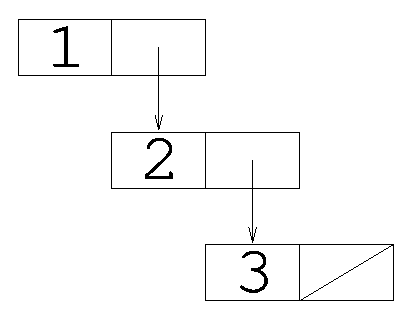
\epsfig{file=cons.ps}}
\end{center}
\end{figure}

List operations are typically implemented in a recursive fashion, where the cdr of the list is taken until the desired element is reached.

\wordtable{
\classword{general-list}{lists}\\
\classword{list}{lists}
}
A \emph{general list} is either the empty list or a cons cell. A \emph{list} is either the empty list or a cons cell whose cdr is also a list. A list is sometimes also known as a \emph{proper list}, and a general list that is not a proper list is known as a \texttt{improper list}. Not all list operations will function given an improper list,
however methods are usually defined on \texttt{general-list} not \texttt{list} since dispatching on \texttt{list} involves a costly check.

\subsubsection{List operations}

\wordtable{
\ordinaryword{>list}{>list ( sequence -- list )}{lists}
}
Turn an arbitrary sequence into a list.
\wordtable{
\ordinaryword{list?}{list?~( obj -- ?~)}{lists}
}
Tests if the object at the top of the stack is a proper list.
\wordtable{
\ordinaryword{unit}{unit ( obj -- [ obj ] )}{lists}
}
Makes a list of one element.
\wordtable{
\ordinaryword{2list}{2list ( o1 o2 -- [ o1 o2 ] )}{lists}
}
Makes a list of two elements.
\wordtable{
\ordinaryword{2unlist}{2unlist ( [ o1 o2 ] -- o1 o2 )}{lists}
}
Pushes the first two elements of a list.
\wordtable{
\ordinaryword{3list}{3list ( o1 o2 o3 -- [ o1 o2 o3 ] )}{lists}
}
Makes a list of three elements.
\wordtable{
\ordinaryword{3unlist}{3unlist ( [ o1 o2 o3 ] -- o1 o2 o3 )}{lists}
}
Pushes the first three elements of a list.
\wordtable{
\ordinaryword{unique}{unique ( obj list -- list )}{lists}
}
If the list already contains an element equal to the object, do nothing, otherwise cons the object into the list.
\wordtable{
\ordinaryword{prune}{prune ( list -- list )}{lists}
}
Removes all duplicates from the list by testing elements for equality.
\wordtable{
\ordinaryword{all=?}{all=?~( list -- ?~)}{lists}
}
Tests if all elements of the list are equal. For the empty list, this is vacuously true.
\wordtable{
\ordinaryword{head}{head~( list n -- list )}{lists}
}
Outputs a new list consisting of the first \texttt{n} elements of \texttt{list}. This allocates memory.
\wordtable{
\ordinaryword{tail}{tail~( list n -- list )}{lists}
}
Outputs a new list consisting of the elements of \texttt{list} from the $n$th index onward. This does not allocate memory; rather it simply takes the \texttt{cdr} \texttt{n} times.
\wordtable{
\ordinaryword{count}{count~( n -- list )}{lists}
}
Return a new list containing all integers from 0 up to $n-1$, inclusive.

\subsubsection{Set-theoretic operations}

\wordtable{
\ordinaryword{contains?}{contains?~( object list -- ?~)}{lists}
}
Tests if \texttt{list} contains an element equal to \texttt{object}.
\wordtable{
\ordinaryword{memq?}{memq?~( object list -- ?~)}{lists}
}
Tests if \texttt{list} contains \texttt{object}. Elements are compared by identity.
\wordtable{
\ordinaryword{contained?}{contained?~( l1 l2 -- ?~)}{lists}
}
Tests if every element of \texttt{l1} is equal to some element of \texttt{l2}.
\wordtable{
\ordinaryword{remove}{remove ( object list -- list )}{lists}
}
Outputs a new list containing all elements of the \texttt{list} except those equal to the \texttt{object}.
\wordtable{
\ordinaryword{remq}{remove ( object list -- list )}{lists}
}
Outputs a new list containing all elements of the \texttt{list} except \texttt{object}. Elements are compared by identity.
\wordtable{
\ordinaryword{intersection}{intersection ( list list -- list )}{lists}
}
Outputs a list of elements present in both lists.
\wordtable{
\ordinaryword{intersection}{difference ( l1 l2 -- list )}{lists}
}
Outputs a list of elements present in \texttt{l2} but not \texttt{l1}.

\subsubsection{List combinators}

\wordtable{
\ordinaryword{each}{each ( list quot -- )}{lists}\\
\texttt{quot:~element --}
}
Applies the quotation to each element of the list.
\wordtable{
\ordinaryword{map}{map ( list quot -- list )}{lists}\\
\texttt{quot:~element -- element}
}
Applies the quotation to each element yielding a new element. The new elements are collected into a new list.
\wordtable{
\ordinaryword{subset}{subset ( list quot -- list )}{lists}\\
\texttt{quot:~element -- ?}
}
Applies the quotation to each element, and outputs a new list containing the elements of the original list for which the quotation output true.
\wordtable{
\ordinaryword{some?}{some?~( list quot -- list )}{lists}\\
\texttt{quot:~element -- ?}
}
Applies the quotation to each element, and outputs the rest of the list upon encountering an element for which the quotation outputs true. If the quotation did not output true for any element, \texttt{some?}~outputs \texttt{f}. Note that the output is a generalized boolean; if the quotation matched any element, the result is true.
\wordtable{
\ordinaryword{all?}{all?~( list quot -- list )}{lists}\\
\texttt{quot:~element -- ?}
}
Outputs \texttt{t} if the quotation yields true when applied to each element, otherwise outputs \texttt{f}. Given the empty list, vacuously outputs \texttt{t}.
\wordtable{
\ordinaryword{sort}{all?~( list quot -- list )}{lists}\\
\texttt{quot:~e1 e2 -- ?}
}
Sorts the list by comparing each pair of elements with the quotation. The quotation should output \texttt{t} if \texttt{e2} is to come before \texttt{e1} in the list. For example, to sort a list of numbers in ascending order, you can do the following:
\begin{alltt}
\textbf{ok} [ 8 6 9 1 10 3 ] [ > ] sort .
[ 1 3 6 8 9 10 ]
\end{alltt}
\wordtable{
\ordinaryword{each-with}{each-with ( object list quot -- )}{lists}\\
\texttt{quot:~object element --}\\
\ordinaryword{map-with}{map-with ( object list quot -- list )}{lists}\\
\texttt{quot:~object element -- element}\\
\ordinaryword{subset-with}{subset-with ( object list quot -- list )}{lists}\\
\texttt{quot:~object element -- ?}\\
\ordinaryword{some-with?}{some-with?~( object list quot -- ?~)}{lists}\\
\texttt{quot:~object element -- ?}\\
\ordinaryword{all-with?}{all-with?~( object list quot -- ?~)}{lists}\\
\texttt{quot:~object element -- ?}
}
Curried forms of the above combinators. They pass an additional object to each invocation of the quotation.

\subsubsection{Queues}

The following set of words manages LIFO (last-in-first-out) queues. Queues are built up from cons cells, and hence are immutable; queue operations always return a new queue.

\wordtable{
\ordinaryword{<queue>}{<queue> ( -- queue )}{lists}
}
Makes a new queue with no elements.
\wordtable{
\ordinaryword{queue-empty?}{queue-empty? ( queue -- ?~)}{lists}
}
Outputs \texttt{t} if the given queue does not contain any elements, \texttt{f} otherwise.
\wordtable{
\ordinaryword{deque}{deque ( queue -- element queue )}{lists}
}
Dequeues an element and outputs a new queue without that element.
\wordtable{
\ordinaryword{enque}{deque ( element queue -- queue )}{lists}
}
Enqueues an element and outputs a new queue.

\subsection{Strings}

\stringglos
\wordtable{
\classword{string}{strings}
}
A string is an immutable sequence of characters. The literal syntax is covered in \ref{string-literals}. Characters do not have a distinct data type, so elements taken out of strings appear as integers on the stack.

\wordtable{
\ordinaryword{string?}{string?~( obj -- ?~)}{strings}
}
Tests if the object at the top of the stack is a string.
%\wordtable{
%\ordinaryword{>string}{>string~( sequence -- string )}{strings}
%}
%Turns any type of sequence with all-integer elements into a string. The integer elements are interpreted as characters.
\wordtable{
\ordinaryword{string-compare}{string-compare~( s1 s2 -- n )}{strings}
}
Compare two strings lexicographically (dictionary order). The output value is one of the following:
\begin{description}
\item[Positive] indicating that \texttt{s1} follows \texttt{s2}
\item[Zero] indicating that \texttt{s1} is equal to \texttt{s2}
\item[Negative] indicating that \texttt{s1} precedes \texttt{s2}
\end{description}
\wordtable{
\ordinaryword{string>}{string> ( s1 s2 -- ?~)}{strings}
}
Tests if \texttt{s1} follows \texttt{s2}. Implemented as follows:
\begin{verbatim}
: string> ( s1 s1 -- ? ) string-compare 0 > ;
\end{verbatim}
This is used to sort lists of strings:
\begin{alltt}
\textbf{ok} [ "Curry" "Apple" "Veal" "Turkey" ] [ string> ] sort .
[ "Apple" "Curry" "Turkey" "Veal" ]
\end{alltt}
\wordtable{
\ordinaryword{fill}{fill~( n char -- string )}{strings}
}
Creates a string with \texttt{char} repeated $n$ times.
\wordtable{
\ordinaryword{pad}{pad~( string n char -- string )}{strings}
}
Creates a string with \texttt{char} repeated $l-n$ times, where $l$ is the length of \texttt{string}. If $l$ is greater than $n$, the empty string is output.

\subsubsection{Substring testing}

\wordtable{
\ordinaryword{string-contains?}{string-contains?~( s1 s2 -- ?~)}{strings}
}
Tests if \texttt{s2} contains \texttt{s1} as a substring.
\wordtable{
\ordinaryword{string-head?}{string-head?~( s1 s2 -- ?~)}{strings}\\
\ordinaryword{string-tail?}{string-tail?~( s1 s2 -- ?~)}{strings}
}
Tests if \texttt{s1} starts or ends with \texttt{s1} as a substring. If \texttt{s1} is longer than \texttt{s2}, outputs \texttt{f}.

\subsubsection{Slicing and splitting}

\wordtable{
\ordinaryword{string/}{string/ ( string n -- s1 s2 )}{strings}
}
Outputs a pair of strings that equal the original string when concatenated. The first string has length $n$, the second has length $l-n$ where $l$ is the length of the input.
\begin{alltt}
\textbf{ok} "Hello world" 5 string .s
\textbf{" world"
"Hello"}
\end{alltt}
\wordtable{
\ordinaryword{string//}{string// ( string n -- s1 s2 )}{strings}
}

Outputs a pair of strings that equal the original string, excluding the $n$th element, when concatenated. The first string has length $n$, the second has length $l-n$ where $l$ is the length of the input.
\begin{alltt}
\textbf{ok} "Hello world" 5 string// .s
\textbf{"world"
"Hello"}
\end{alltt}
\wordtable{
\ordinaryword{?string-head}{?string-head~( s1 s2 -- string ?~)}{strings}\\
\ordinaryword{?string-tail}{?string-tail~( s1 s2 -- string ?~)}{strings}
}
Tests if \texttt{s1} starts or ends with \texttt{s1} as a substring. If there is a match, outputs the subrange of \texttt{s1} excluding \texttt{s1} followed by \texttt{t}. If there is no match, outputs \texttt{s1} followed by \texttt{f}/
\wordtable{
\ordinaryword{split1}{split1~( str split -- before after )}{strings}
}
If \texttt{string} does not contain \texttt{split} as a substring, then \texttt{before} is equal to the \texttt{string}, and \texttt{after} is \texttt{f}. Otherwise, \texttt{before} and \texttt{after} are both strings, and yield the input excluding \texttt{split} when concatenated.
\wordtable{
\ordinaryword{split}{split~( str split -- list )}{strings}
}
Outputs a list of substrings taken between occurrences of \texttt{split} in \texttt{string}. If \texttt{split} does not occur inside \texttt{string}, outputs a singleton list containing \texttt{string} only.
\begin{alltt}
\textbf{ok} "/usr/local/bin" CHAR: / split .
\textbf{[ "" "usr" "local" "bin" ]}
\end{alltt}
\wordtable{
\ordinaryword{split-n}{split-n~( str n -- list )}{strings}
}
Splits the string into groups of \texttt{n} characters and collects them in a list. If the string's length is not a multiple of \texttt{n}, the final string in the list might be shorter.

\subsubsection{Characters}

\wordtable{
\ordinaryword{ch>string}{ch>string ( n -- string )}{strings}
}
Turns an integer representing a character value into a single-element string.
\wordtable{
\ordinaryword{blank?}{blank?~( n -- ?~)}{strings}\\
\ordinaryword{letter?}{letter?~( n -- ?~)}{strings}\\
\ordinaryword{LETTER?}{LETTER?~( n -- ?~)}{strings}\\
\ordinaryword{digit?}{digit?~( n -- ?~)}{strings}\\
\ordinaryword{printable?}{printable?~( n -- ?~)}{strings}\\
\ordinaryword{quotable?}{quotable?~( n -- ?~)}{strings}\\
\ordinaryword{url-quotable?}{url-quotable?~( n -- ?~)}{strings}
}
Various character classification predicates.

\subsection{String buffers}

\sbufglos
\wordtable{
\classword{sbuf}{strings}
}
A string buffer is a mutable and growable sequence of characters. String buffers can be used to construct new strings by accumilating substrings and characters, however usually they are only used indirectly, since the sequence construction words in \ref{make-seq} are more convenient to use in many cases.
\wordtable{
\ordinaryword{sbuf?}{sbuf?~( object -- ?~)}{strings}
}
Tests if the object at the top of the stack is a string buffer.
\wordtable{
\ordinaryword{>sbuf}{>sbuf~( sequence -- sbuf )}{strings}
}
Turns any type of sequence into a string buffer. Given a string buffer, this makes a fresh copy
\wordtable{
\ordinaryword{sbuf>string}{sbuf>string~( sbuf -- string )}{strings}
}
Turns a string buffer into a string holding the same characters.

\subsection{\label{make-seq}Constructing sequences}

The library supports an idiom where sequences can be constructed without passing the partial sequence being built on the stack. This reduces stack noise, and thus simplifies code and makes it easier to understand.

\newcommand{\dynamicscopeglos}{\glossary{
name=dynamic scope,
description={a variable binding policy where bindings established in a scope are visible to all code executed while the scope is active}}}
\dynamicscopeglos
\wordtable{
\ordinaryword{make-list}{make-list ( quot -- list )}{namespaces}\\
\ordinaryword{make-string}{make-string ( quot -- string )}{namespaces}\\
\ordinaryword{make-sbuf}{make-sbuf ( quot -- string )}{namespaces}\\
\ordinaryword{make-vector}{make-vector ( quot -- vector )}{namespaces}
}
Calls the quotation in a new \texttt{dynamic scope}. The quotation and any words it calls can execute the \texttt{,} and \texttt{\%} words to add elements at the end of the sequence being constructed.
\wordtable{
\ordinaryword{,}{,~( element -- )}{namespaces}
}
Adds the element to the end of the sequence being constructed by the innermost call to one of the above combinators.
\wordtable{
\ordinaryword{unique,}{unique,~( element -- )}{namespaces}
}
Adds the element to the end of the sequence being constructed as long as the sequence does not already have an equal element.
\wordtable{
\ordinaryword{literal,}{literal,~( element -- )}{namespaces}
}
Adds the element wrapped inside a one-element list, then adds the \texttt{car} word. This is used to construct quotations with \texttt{make-list} that must push a word on the stack.
\wordtable{
\ordinaryword{\%}{\% ( sequence -- )}{namespaces}
}
Appends the subsequence to the end of the sequence being constructed.

Note that the sequence construction combinators will capture any variables set inside the quotation, due to the dynamic scoping behavior. These combinators are actually implemented using variables. See \ref{namespaces}.

\section{Mappings}

\glossary{name=mapping,
description={an unordered collection of elements, accessed by key. Examples include association lists and hashtables}}

Mappings associate keys with values. The two classes of mappings in the Factor library are association lists and hashtables.

\begin{tabular}[t]{l|c|c|c|l}
Class&Mutable&Ordered&Lookup&Primary purpose\\
\hline
\texttt{assoc}&&$\surd$&$O(n)$&Small, unchanging mappings\\
\texttt{hashtable}&$\surd$&&$O(1)$&Large or frequently-changing mappings
\end{tabular}

It might be tempting to just always use hashtables, however for very small mappings, association lists are just as efficient, and are easier to work with since the entire set of list words can be used with them.

\subsection{Association lists}

\glossary{name=association list,
description={a list of pairs, where the car if each pair is a key and the cdr is the value associated with that key}}

Association lists are built from cons cells. They are structured like a ribbed spine, where the ``spine'' is a list and each ``rib'' is a cons cell holding a key/value pair.

\wordtable{
\ordinaryword{assoc?}{assoc ( object -- ?~)}{lists}
}
Tests if the object at the top of the stack is a proper list whose every element is a cons.

\wordtable{
\ordinaryword{assoc}{assoc ( k alist -- v )}{lists}\\
\ordinaryword{assoc*}{assoc* ( k alist -- [[ k v ]] )}{lists}
}
These words look up a key in an association list, comparing keys in the list with the given key by equality with \texttt{=}. The list is searched starting from the beginning. The two words differ in that the latter returns the key/value pair located, whereas the former only returns the value. The \texttt{assoc*} word allows a distinction to be made between a missing value and a value equal to \texttt{f}, since in the case of a missing value it outputs \texttt{f}.
\wordtable{
\ordinaryword{assq}{assq ( k alist -- v )}{lists}\\
\ordinaryword{assq*}{assq* ( k alist -- [[ k v ]] )}{lists}
}
These words compare keys by identity with \texttt{eq?}~and are dual to \texttt{assoc} and \texttt{assoc*}.
\wordtable{
\ordinaryword{acons}{acons ( v k alist -- alist )}{lists}\\
\ordinaryword{set-assoc}{set-assoc ( v k alist -- alist )}{lists}
}
These words output a new association list containing the key/value pair.
They differ in that \texttt{set-assoc} removes any existing key/value pairs with the given key first. In both cases, searching for the key in the returned association list gives the new value, however with the slightly faster \texttt{acons}, the old value remains shadowed in the list.
\wordtable{
\ordinaryword{remove-assoc}{remove-assoc ( k alist -- alist )}{lists}
}
Outputs a new association list which does not have any key/value pairs with the key equal to \texttt{k}.

\begin{figure}
\caption{An association list and its graphical representation}
\begin{verbatim}
[
    [[ "Salsa" "Hot" ]]
    [[ "Stir-Fry" "Medium" ]]
    [[ "Peppers" "Very Hot" ]]
]
\end{verbatim}

\begin{center}
\scalebox{0.45}{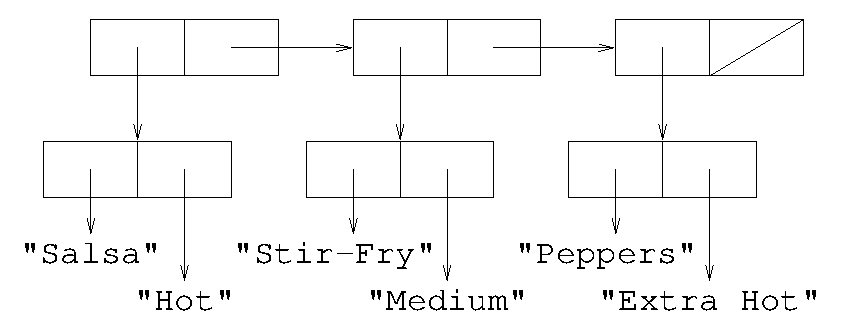
\epsfig{file=assoc.eps}}
\end{center}
\end{figure}

\subsubsection{Dual representation}

Sometimes it is convenient to decompose an association list into two lists of equal length, containing the keys and values, respectively, in the same order as the association list. This dual representation can be manipulated with a handful of helper words.

\wordtable{
\ordinaryword{zip}{zip ( keys values -- alist )}{lists}\\
\ordinaryword{unzip}{unzip ( alist -- keys values )}{lists}
}
These words convert between pairs of lists and lists of pairs.
\begin{alltt}
\textbf{ok} [ 1 2 3 ] [ 4 5 6 ] zip .
[ [[ 1 4 ]] [[ 2 5 ]] [[ 3 6 ]] ]
\textbf{ok} [ [[ 1 2 ]] [[ 3 4 ]] [[ 5 6 ]] ] unzip .s
[ 2 4 6 ]
[ 1 3 5 ]
\end{alltt}
\wordtable{
\ordinaryword{2cons}{2cons ( car1 car2 cdr1 cdr2 -- c1 c2 )}{lists}
}
Cons a pair of elements onto a pair of lists.
\wordtable{
\ordinaryword{2car}{2car ( c1 c2 -- car1 car2 )}{lists}\\
\ordinaryword{2cdr}{2cdr ( c1 c2 -- cdr1 cdr2 )}{lists}
}
Deconstructs paired lists.

\subsection{Hashtables}

\wordtable{
\classword{hashtable}{hashtables}
}


\subsection{\label{namespaces}Namespaces}

\section{Mathematics}

\numberglos

\begin{figure}
\begin{center}
\caption{Numerical class hierarchy}
\scalebox{0.5}{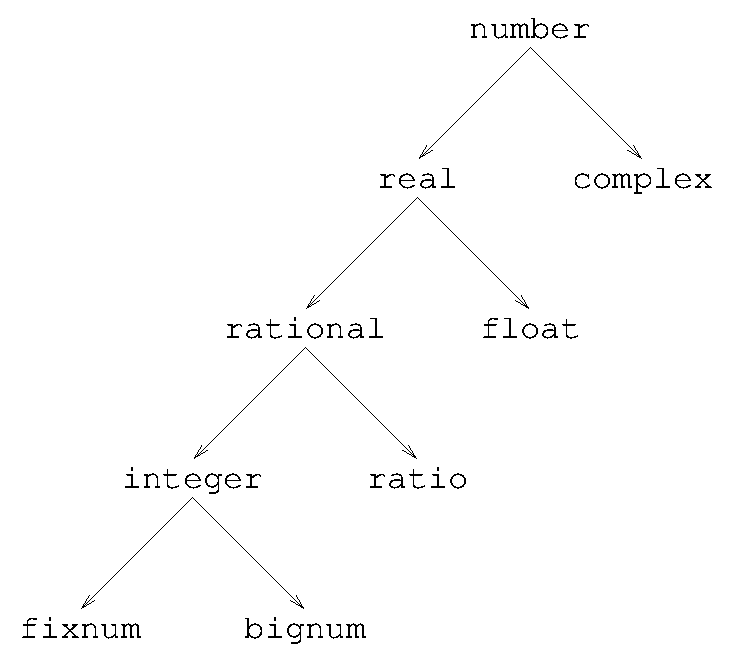
\epsfig{file=number.ps}}
\end{center}
\end{figure}

Factor's numbers more closely model the mathematical concept of a number than other languages. Where possible, exact answers are given -- for example, adding or multiplying two integers never results in overflow, and dividing two integers yields a fraction rather than a truncated result. Complex numbers are supported, allowing many functions to be computed with parameters that would raise errors or return ``not a number'' in other languages.

\subsection{Integers}

\integerglos

The simplest type of number is the integer. Integers come in two varieties -- \emph{fixnums} and \emph{bignums}. As their names suggest, a fixnum is a fixed-width quantity\footnote{Fixnums range in size from $-2^{w-3}-1$ to $2^{w-3}$, where $w$ is the word size of your processor (for example, 32 bits). Because fixnums automatically grow to bignums, usually you do not have to worry about details like this.}, and is a bit quicker to manipulate than an arbitrary-precision bignum.

The predicate word \texttt{integer?}~tests if the top of the stack is an integer. If this returns true, then exactly one of \texttt{fixnum?}~or \texttt{bignum?}~would return true for that object. Usually, your code does not have to worry if it is dealing with fixnums or bignums.

Unlike some languages where the programmer has to declare storage size explicitly and worry about overflow, integer operations automatically return bignums if the result would be too big to fit in a fixnum. Here is an example where multiplying two fixnums returns a bignum:

\begin{alltt}
\textbf{ok} 134217728 fixnum? .
\textbf{t}
\textbf{ok} 128 fixnum? .
\textbf{t}
\textbf{ok} 134217728 128 * .
\textbf{17179869184}
\textbf{ok} 134217728 128 * bignum? .
\textbf{t}
\end{alltt}

Integers can be entered using a different base. By default, all number entry is in base 10, however this can be changed by prefixing integer literals with one of the parsing words \texttt{BIN:}, \texttt{OCT:}, or \texttt{HEX:}. For example:

\begin{alltt}
\textbf{ok} BIN: 1110 BIN: 1 + .
\textbf{15}
\textbf{ok} HEX: deadbeef 2 * .
\textbf{7471857118}
\end{alltt}

The word \texttt{.} prints numbers in decimal, regardless of how they were input. A set of words in the \texttt{prettyprint} vocabulary is provided for print integers using another base.

\begin{alltt}
\textbf{ok} 1234 .h
\textbf{4d2}
\textbf{ok} 1234 .o
\textbf{2232}
\textbf{ok} 1234 .b
\textbf{10011010010}
\end{alltt}

\subsection{Rational numbers}

\newcommand{\rationalglos}{\glossary{
name=rational,
description={an instance of the \texttt{rational} class, which is a disjoint union of the
\texttt{integer} and \texttt{ratio} classes}}}
\rationalglos
\ratioglos

If we add, subtract or multiply any two integers, the result is always an integer. However, this is not the case with division. When dividing a numerator by a denominator where the numerator is not a integer multiple of the denominator, a ratio is returned instead.

\begin{alltt}
1210 11 / .
\emph{110}
100 330 / .
\emph{10/33}
\end{alltt}

Ratios are printed and can be input literally in the form of the second example. Ratios are always reduced to lowest terms by factoring out the greatest common divisor of the numerator and denominator. A ratio with a denominator of 1 becomes an integer. Trying to create a ratio with a denominator of 0 raises an error.

The predicate word \texttt{ratio?}~tests if the top of the stack is a ratio. The predicate word \texttt{rational?}~returns true if and only if one of \texttt{integer?}~or \texttt{ratio?}~would return true for that object. So in Factor terms, a ``ratio'' is a rational number whose denominator is not equal to 1.

Ratios behave just like any other number -- all numerical operations work as expected, and in fact they use the formulas for adding, subtracting and multiplying fractions that you learned in high school.

\begin{alltt}
\textbf{ok} 1/2 1/3 + .
\textbf{5/6}
\textbf{ok} 100 6 / 3 * .
\textbf{50}
\end{alltt}

Ratios can be deconstructed into their numerator and denominator components using the \texttt{numerator} and \texttt{denominator} words. The numerator and denominator are both integers, and furthermore the denominator is always positive. When applied to integers, the numerator is the integer itself, and the denominator is 1.

\begin{alltt}
\textbf{ok} 75/33 numerator .
\textbf{25}
\textbf{ok} 75/33 denominator .
\textbf{11}
\textbf{ok} 12 numerator .
\textbf{12}
\end{alltt}

\subsection{Floating point numbers}

\newcommand{\realglos}{\glossary{
name=real,
description={an instance of the \texttt{real} class, which is a disjoint union of the
\texttt{rational} and \texttt{float} classes}}}
\realglos
\floatglos

Rational numbers represent \emph{exact} quantities. On the other hand, a floating point number is an \emph{approximation}. While rationals can grow to any required precision, floating point numbers are fixed-width, and manipulating them is usually faster than manipulating ratios or bignums (but slower than manipulating fixnums). Floating point literals are often used to represent irrational numbers, which have no exact representation as a ratio of two integers. Floating point literals are input with a decimal point.

\begin{alltt}
\textbf{ok} 1.23 1.5 + .
\textbf{1.73}
\end{alltt}

The predicate word \texttt{float?}~tests if the top of the stack is a floating point number. The predicate word \texttt{real?}~returns true if and only if one of \texttt{rational?}~or \texttt{float?}~would return true for that object.

Floating point numbers are \emph{contagious} -- introducing a floating point number in a computation ensures the result is also floating point.

\begin{alltt}
\textbf{ok} 5/4 1/2 + .
\textbf{7/4}
\textbf{ok} 5/4 0.5 + .
\textbf{1.75}
\end{alltt}

Apart from contaigion, there are two ways of obtaining a floating point result from a computation; the word \texttt{>float ( n -{}- f )} converts a rational number into its floating point approximation, and the word \texttt{/f ( x y -{}- x/y )} returns the floating point approximation of a quotient of two numbers.

\begin{alltt}
\textbf{ok} 7 4 / >float .
\textbf{1.75}
\textbf{ok} 7 4 /f .
\textbf{1.75}
\end{alltt}

Indeed, the word \texttt{/f} could be defined as follows:

\begin{alltt}
: /f / >float ;
\end{alltt}

However, the actual definition is slightly more efficient, since it computes the floating point result directly.

\subsection{Complex numbers}

Complex numbers arise as solutions to quadratic equations whose graph does not intersect the x axis. For example, the equation $x^2 + 1 = 0$ has no solution for real $x$, because there is no real number that is a square root of -1. However, in the field of complex numbers, this equation has a well-known solution:

\begin{alltt}
\textbf{ok} -1 sqrt .
\textbf{\#\{ 0 1 \}}
\end{alltt}

The literal syntax for a complex number is \texttt{\#\{ re im \}}, where \texttt{re} is the real part and \texttt{im} is the imaginary part. For example, the literal \texttt{\#\{ 1/2 1/3 \}} corresponds to the complex number $1/2 + 1/3i$.

The words \texttt{i} an \texttt{-i} push the literals \texttt{\#\{ 0 1 \}} and \texttt{\#\{ 0 -1 \}}, respectively.

The predicate word \texttt{complex?} tests if the top of the stack is a complex number. Note that unlike math, where all real numbers are also complex numbers, Factor only considers a number to be a complex number if its imaginary part is non-zero.

Complex numbers can be deconstructed into their real and imaginary components using the \texttt{real} and \texttt{imaginary} words. Both components can be pushed at once using the word \texttt{>rect ( z -{}- re im )}.

\begin{alltt}
\textbf{ok} -1 sqrt real .
\textbf{0}
\textbf{ok} -1 sqrt imaginary .
\textbf{1}
\textbf{ok} -1 sqrt sqrt >rect .s
\textbf{\{ 0.7071067811865476 0.7071067811865475 \}}
\end{alltt}

A complex number can be constructed from a real and imaginary component on the stack using the word \texttt{rect> ( re im -{}- z )}.

\begin{alltt}
\textbf{ok} 1/3 5 rect> .
\textbf{\#\{ 1/3 5 \}}
\end{alltt}

Complex numbers are stored in \emph{rectangular form} as a real/imaginary component pair (this is where the names \texttt{>rect} and \texttt{rect>} come from). An alternative complex number representation is \emph{polar form}, consisting of an absolute value and argument. The absolute value and argument can be computed using the words \texttt{abs} and \texttt{arg}, and both can be pushed at once using \texttt{>polar ( z -{}- abs arg )}.

\begin{alltt}
\textbf{ok} 5.3 abs .
\textbf{5.3}
\textbf{ok} i arg .
\textbf{1.570796326794897}
\textbf{ok} \#\{ 4 5 \} >polar .s
\textbf{\{ 6.403124237432849 0.8960553845713439 \}}
\end{alltt}

A new complex number can be created from an absolute value and argument using \texttt{polar> ( abs arg -{}- z )}.

\begin{alltt}
\textbf{ok} 1 pi polar> .
\textbf{\#\{ -1.0 1.224606353822377e-16 \}}
\end{alltt}

\subsection{Transcedential functions}

The \texttt{math} vocabulary provides a rich library of mathematical functions that covers exponentiation, logarithms, trigonometry, and hyperbolic functions. All functions accept and return complex number arguments where appropriate. These functions all return floating point values, or complex numbers whose real and imaginary components are floating point values.

\texttt{\^{} ( x y -- x\^{}y )} raises \texttt{x} to the power of \texttt{y}. In the cases of \texttt{y} being equal to $1/2$, -1, or 2, respectively, the words \texttt{sqrt}, \texttt{recip} and \texttt{sq} can be used instead.

\begin{alltt}
\textbf{ok} 2 4 \^ .
\textbf{16.0}
\textbf{ok} i i \^ .
\textbf{0.2078795763507619}
\end{alltt}

All remaining functions have a stack effect \texttt{( x -{}- y )}, it won't be repeated for brevity.

\texttt{exp} raises the number $e$ to a specified power. The number $e$ can be pushed on the stack with the \texttt{e} word, so \texttt{exp} could have been defined as follows:

\begin{alltt}
: exp ( x -- e^x ) e swap \^ ;
\end{alltt}

However, it is actually defined otherwise, for efficiency.\footnote{In fact, the word \texttt{\^{}} is actually defined in terms of \texttt{exp}, to correctly handle complex number arguments.}

\texttt{log} computes the natural (base $e$) logarithm. This is the inverse of the \texttt{exp} function.

\begin{alltt}
\textbf{ok} -1 log .
\textbf{\#\{ 0.0 3.141592653589793 \}}
\textbf{ok} e log .
\textbf{1.0}
\end{alltt}

\texttt{sin}, \texttt{cos} and \texttt{tan} are the familiar trigonometric functions, and \texttt{asin}, \texttt{acos} and \texttt{atan} are their inverses.

The reciprocals of the sine, cosine and tangent are defined as \texttt{sec}, \texttt{cosec} and \texttt{cot}, respectively. Their inverses are \texttt{asec}, \texttt{acosec} and \texttt{acot}.

\texttt{sinh}, \texttt{cosh} and \texttt{tanh} are the hyperbolic functions, and \texttt{asinh}, \texttt{acosh} and \texttt{atanh} are their inverses.

Similarly, the reciprocals of the hyperbolic functions are defined as \texttt{sech}, \texttt{cosech} and \texttt{coth}, respectively. Their inverses are \texttt{asech}, \texttt{acosech} and \texttt{acoth}.

\subsection{Modular arithmetic}

In addition to the standard division operator \texttt{/}, there are a few related functions that are useful when working with integers.

\texttt{/i ( x y -{}- x/y )} performs a truncating integer division. It could have been defined as follows:

\begin{alltt}
: /i / >integer ;
\end{alltt}

However, the actual definition is a bit more efficient than that.

\texttt{mod ( x y -{}- x\%y )} computes the remainder of dividing \texttt{x} by \texttt{y}. If the result is 0, then \texttt{x} is a multiple of \texttt{y}.

\texttt{/mod ( x y -{}- x/y x\%y )} pushes both the quotient and remainder.

\begin{alltt}
\textbf{ok} 100 3 mod .
\textbf{1}
\textbf{ok} -546 34 mod .
\textbf{-2}
\end{alltt}

\texttt{gcd ( x y -{}- z )} pushes the greatest common divisor of two integers; that is, the largest number that both integers could be divided by and still yield integers as results. This word is used behind the scenes to reduce rational numbers to lowest terms when doing ratio arithmetic.

\subsection{Bitwise operations}

There are two ways of looking at an integer -- as a mathematical entity, or as a string of bits. The latter representation faciliates the so-called \emph{bitwise operations}.

\texttt{bitand ( x y -{}- x\&y )} returns a new integer where each bit is set if and only if the corresponding bit is set in both $x$ and $y$. If you're considering an integer as a sequence of bit flags, taking the bitwise-and with a mask switches off all flags that are not explicitly set in the mask.

\begin{alltt}
BIN: 101 BIN: 10 bitand .b
\emph{0}
BIN: 110 BIN: 10 bitand .b
\emph{10}
\end{alltt}

\texttt{bitor ( x y -{}- x|y )} returns a new integer where each bit is set if and only if the corresponding bit is set in at least one of $x$ or $y$. If you're considering an integer as a sequence of bit flags, taking the bitwise-or with a mask switches on all flags that are set in the mask.

\begin{alltt}
BIN: 101 BIN: 10 bitor .b
\emph{111}
BIN: 110 BIN: 10 bitor .b
\emph{110}
\end{alltt}

\texttt{bitxor ( x y -{}- x\^{}y )} returns a new integer where each bit is set if and only if the corresponding bit is set in exactly one of $x$ or $y$. If you're considering an integer as a sequence of bit flags, taking the bitwise-xor with a mask toggles on all flags that are set in the mask.

\begin{alltt}
BIN: 101 BIN: 10 bitxor .b
\emph{111}
BIN: 110 BIN: 10 bitxor .b
\emph{100}
\end{alltt}

\texttt{bitnot ( x -{}- y )} returns the bitwise complement of the input; that is, each bit in the input number is flipped. This is actually equivalent to negating a number, and subtracting one. So indeed, \texttt{bitnot} could have been defined as thus:

\begin{alltt}
: bitnot neg pred ;
\end{alltt}

\texttt{shift ( x n -{}- y )} returns a new integer consisting of the bits of the first integer, shifted to the left by $n$ positions. If $n$ is negative, the bits are shifted to the right instead, and bits that ``fall off'' are discarded.

\begin{alltt}
BIN: 101 5 shift .b
\emph{10100000}
BIN: 11111 -2 shift .b
\emph{111}
\end{alltt}

The attentive reader will notice that shifting to the left is equivalent to multiplying by a power of two, and shifting to the right is equivalent to performing a truncating division by a power of two.

\chapter{The development environment}

Factor supports interactive development in a live environment. Instead of working with
static executable files and restarting your application after each change, you can
incrementally make changes to your application and test them immediately. If you
notice an undesirable behavior, Factor's powerful reflection features will aid in
pinpointing the error.

If you are used to a statically typed language, you might find Factor's tendency to only fail at runtime hard to work with at first. However, the interactive development tools outlined in this document allow a much quicker turn-around time for testing changes. Also, write unit tests -- unit testing is a great way to ensure that old bugs do not re-appear once they've been fixed.

\section{System organization}

\subsection{The listener}

Factor is an \emph{image-based environment}. When you compiled Factor, you also generated a file named \texttt{factor.image}. I will have more to say about images later, but for now it suffices to understand that to start Factor, you must pass the image file name on the command line:
\begin{alltt}
./f factor.image
\textbf{Loading factor.image... relocating... done
Factor 0.73 :: http://factor.sourceforge.net :: unix/x86
(C) 2003, 2005 Slava Pestov, Chris Double,
Mackenzie Straight
ok}
\end{alltt}
An \texttt{\textbf{ok}} prompt is printed after the initial banner, indicating the listener is ready to execute Factor phrases. The listener is a piece of Factor code, like any other; however, it helps to think of it as the primary interface to the Factor system. The listener reads Factor code and executes it. You can try the classical first program:

\begin{alltt}
\textbf{ok} "Hello, world." print
\textbf{Hello, world.}
\end{alltt}


Multi-line phrases are supported; if there are unclosed brackets, the listener outputs \texttt{...} instead of the \texttt{ok} prompt, and the entire phrase is executed once all brackets are closed:

\begin{alltt}
\textbf{ok} [ 1 2 3 ] [
\textbf{...} .
\textbf{...} ] each
\textbf{1
2
3}
\end{alltt}

The listener knows when to print a continuation prompt by looking at the height of the
stack. Parsing words such as \texttt{[} and \texttt{:} leave elements on the parser
stack; these elements are popped by \texttt{]} and \texttt{;}.

\subsection{Source files}

While it is possible to do all development in the listener and save your work in images, it is far more convenient to work with source files, at least until an in-image structure editor is developed.

By convention, Factor source files are saved with the \texttt{.factor} filename extension. They can be loaded into the image as follows:

\begin{alltt}
\textbf{ok} "examples/numbers-game.factor" run-file
\end{alltt}

In Factor, loading a source file replaces any existing definitions\footnote{But see \ref{compiler} for this is not true of compiled code.}. Each word definition remembers what source file it was loaded from (if any). To reload the source file associated with a definition, use the \texttt{reload} word:

\begin{alltt}
\textbf{ok} \bs draw reload
\end{alltt}

Word definitions also retain the line number where they are located in their original source file. This allows you to open a word definition in jEdit\footnote{\texttt{http://www.jedit.org}} for editing using the
\texttt{jedit} word:

\begin{alltt}
\textbf{ok} \bs compile jedit
\end{alltt}

This word requires that a jEdit instance is already running.

For the \texttt{jedit} word to work with words in the Factor library, you must set the \texttt{"resource-path"} variable to the location of the Factor source tree. One way to do this is to add a phrase like the following to your \texttt{.factor-rc}:

\begin{verbatim}
"/home/slava/Factor/" "resource-path" set
\end{verbatim}

On startup, Factor reads the \texttt{.factor-rc} file from your home directory. You can put
any quick definitions you want available at the listener there. To avoid loading this
file, pass the \texttt{-no-user-init} command line switch. Another way to have a set of definitions available at all times is to save a custom image, as described in the next section.

\subsection{Images}

The \texttt{factor.image} file is basically a dump of all objects in the heap. A new image can be saved as follows:

\begin{alltt}
\textbf{ok} "work.image" save-image
\textbf{Saving work.image...}
\end{alltt}

When you save an image before exiting Factor, then start Factor again, everything will be almost as you left it. Try the following:

\begin{alltt}
./f factor.image
\textbf{ok} "Learn Factor" "reminder" set
\textbf{ok} "factor.image" save-image bye
\textbf{Saving factor.image...}
\end{alltt}

Factor will save the image and exit. Now start it again and see that the reminder is still there:

\begin{alltt}
./f factor.image
\textbf{ok} "reminder" get .
\textbf{"Learn Factor"}
\end{alltt}

This is what is meant by the image being an \emph{infinite session}. When you shut down and restart Factor, what happends is much closer to a Laptop's ``suspend'' mode, than a desktop computer being fully shut down.

\subsection{Looking at objects}

Probably the most important debugging tool of them all is the \texttt{.} word. It prints the object at the top of the stack in a form that can be parsed by the Factor parser. A related word is \texttt{prettyprint}. It is identical to \texttt{.} except the output is more verbose; lists, vectors and hashtables are broken up into multiple lines and indented.

\begin{alltt}
\textbf{ok} [ [ \tto 1 \ttc \tto 2 \ttc ] dup car swap cdr ] .
[ [ \tto 1 \ttc \tto 2 \ttc ] dup car swap cdr ]
\end{alltt}

Most objects print in a parsable form, but not all. One exceptions to this rule is objects with external state, such as I/O ports or aliens (pointers to native structures). Also, objects with circular or very deeply nested structure will not print in a fully parsable form, since the prettyprinter has a limit on maximum nesting. Here is an example -- a vector is created, that holds a list whose first element is the vector itself:

\begin{alltt}
\textbf{ok} \tto \ttc [ unit 0 ] keep [ set-vector-nth ] keep .
\tto [ ... ] \ttc
\end{alltt}

The prettyprinted form of a vector or list with many elements is not always readable. The \texttt{[.]} and \texttt{\tto.\ttc} words output a list or a vector, respectively, with each element on its own line. In fact, the stack printing words are defined in terms of \texttt{[.]} and \texttt{\tto.\ttc}:

\begin{verbatim}
: .s datastack  {.} ;
: .r callstack  {.} ;
: .n namestack  [.] ;
: .c catchstack [.] ;
\end{verbatim}

Before we move on, one final set of output words comes is used to output integers in
different numeric bases. The \texttt{.b} word prints an integer in binary, \texttt{.o} in octal, and \texttt{.h} in hexadecimal.

\begin{alltt}
\textbf{ok} 31337 .b
\textbf{111101001101001}
\textbf{ok} 31337 .o
\textbf{75151}
\textbf{ok} 31337 .h
\textbf{7a69}
\end{alltt}

\section{Word tools}

\subsection{Exploring vocabularies}

Factor organizes code in a two-tier structure of vocabularies and words. A word is the smallest unit of code; it corresponds to a function or method in other languages. Vocabularies group related words together for easy browsing and tracking of source dependencies.

Entering \texttt{vocabs .}~in the listener produces a list of all existing vocabularies:

\begin{alltt}
\textbf{ok} vocabs .
\textbf{[ "alien" "ansi" "assembler" "browser-responder"
"command-line" "compiler" "cont-responder" "errors"
"file-responder" "files" "gadgets" "generic"
"hashtables" "html" "httpd" "httpd-responder" "image"
"inference" "interpreter" "io-internals" "jedit"
"kernel" "kernel-internals" "line-editor" "listener"
"lists" "logging" "math" "math-internals" "memory"
"namespaces" "parser" "prettyprint" "profiler"
"quit-responder" "random" "resource-responder"
"scratchpad" "sdl" "shells" "stdio" "streams"
"strings" "syntax" "telnetd" "test" "test-responder"
"threads" "unparser" "url-encoding" "vectors" "words" ]}
\end{alltt}

As you can see, there are a lot of vocabularies! Now, you can use \texttt{words .}~to list the words inside a given vocabulary:

\begin{alltt}
\textbf{ok} "namespaces" words .
\textbf{[ (get) , <namespace> >n append, bind change cons@
dec extend get global inc init-namespaces list-buffer
literal, make-list make-rlist make-rstring make-string
make-vector n> namespace namestack nest off on put set
set-global set-namestack unique, unique@ with-scope ]}
\end{alltt}

You can look at the definition of any word, including library words, using \texttt{see}. Keep in mind you might have to \texttt{USE:} the vocabulary first.

\begin{alltt}
\textbf{ok} USE: httpd
\textbf{ok} \bs httpd-connection see
\textbf{IN: httpd : httpd-connection ( socket -- )
    "http-server" get accept [
        httpd-client
    ] in-thread drop ;}
\end{alltt}

The \texttt{see} word shows a reconstruction of the source code, not the original source code. So in particular, formatting and some comments are lost.

\subsection{Cross-referencing words}

The \texttt{apropos.} word is handy when searching for related words. It lists all words
whose names contain a given string. The \texttt{apropos.} word is also useful when you know the exact name of a word, but are unsure what vocabulary it is in. For example, if you're looking for ways to iterate over various collections, you can do an apropos search for \texttt{map}:

\begin{alltt}
\textbf{ok} "map" apropos.
\textbf{IN: inference
type-value-map
IN: lists
map
map-with
IN: sdl
set-surface-map
surface-map
IN: strings
string-map
IN: vectors
vector-map}
\end{alltt}

From the above output, you can see that \texttt{map} is for lists, \texttt{string-map} is for strings, and \texttt{vector-map} is for vectors.

The \texttt{usage} word finds all words that refer to a given word and pushes a list on the stack. This word is helpful in two situations; the first is for learning -- a good way to learn a word is to see it used in context. The second is during refactoring -- if you change a word's stack effect, you must also update all words that call it. Usually you print the
return value of \texttt{usage} using \texttt{.}:

\begin{alltt}
\textbf{ok} \bs string-map usage .
\textbf{schars>entities
filter-null
url-encode}
\end{alltt}

Another useful word is \texttt{usages}. Unlike \texttt{usage}, it finds all usages, even
indirect ones -- so if a word refers to another word that refers to the given word,
both words will be in the output list.

\subsection{Exploring classes}

Factor supports object-oriented programming via generic words. Generic words are called
like ordinary words, however they can have multiple definitions, one per class, and
these definitions do not have to appear in the same source file. Such a definition is
termed a \emph{method}, and the method is said to \emph{specialize} on a certain
class. A class in the most
general sense is just a set of objects. You can output a list of classes in the system
with \texttt{classes .}:

\begin{alltt}
\textbf{ok} classes.
\textbf{[ alien alien-error byte-array displaced-alien
dll ansi-stream disp-only displaced indirect operand
register absolute absolute-16/16 relative relative-bitfld
item kernel-error no-method border checkbox dialog editor
ellipse etched-rect frame gadget hand hollow-ellipse
hollow-rect label line menu pane pile plain-ellipse
plain-rect rectangle roll-rect scroller shelf slider
stack tile viewport world 2generic arrayed builtin
complement generic null object predicate tuple
tuple-class union hashtable html-stream class-tie
computed inference-error inference-warning literal
literal-tie value buffer port jedit-stream boolean
general-t array cons general-list list bignum complex
fixnum float integer number ratio rational real
parse-error potential-float potential-ratio
button-down-event button-up-event joy-axis-event
joy-ball-event joy-button-down-event joy-button-up-event
joy-hat-event key-down-event key-up-event motion-event
quit-event resize-event user-event sequence stdio-stream
client-stream fd-stream null-stream server string-output
wrapper-stream LETTER blank digit letter printable sbuf
string text POSTPONE: f POSTPONE: t vector compound
primitive symbol undefined word ]}
\end{alltt}

If you \texttt{see} a generic word, all methods defined on the generic word are shown.
Alternatively, you can use \texttt{methods.} to print all methods specializing on a
given class:

\begin{alltt}
\textbf{ok} \bs list methods.
\textbf{PREDICATE: general-list list
    dup [
        last* cdr
    ] when not ;
IN: gadgets
M: list custom-sheet
    [
        length count
    ] keep zip alist>sheet "Elements:" <titled> ;
IN: prettyprint
M: list prettyprint*
    [
        [
            POSTPONE: [
        ] car swap [
            POSTPONE: ]
        ] car prettyprint-sequence
    ] check-recursion ;}
\end{alltt}

\subsection{Browsing via the HTTP server}


A more sophisticated way to browse the library is using the integrated HTTP server. You can start the HTTP server using the following pair of commands:

\begin{alltt}
\textbf{ok} USE: httpd
\textbf{ok} 8888 httpd
\end{alltt}

Then, point your browser to the following URL, and start browsing:

\begin{quote}
\texttt{http://localhost:8888/responder/inspect/vocabularies}
\end{quote}

To stop the HTTP server, point your browser to

\begin{quote}
\texttt{http://localhost:8888/responder/quit}.
\end{quote}

You can even start the HTTP in a separate thread, and look at code in your web browser while continuing to play in the listener:

\begin{alltt}
\textbf{ok} USE: httpd
\textbf{ok} USE: threads
\textbf{ok} [ 8888 httpd ] in-thread
\end{alltt}

\section{Dealing with runtime errors}

\subsection{Looking at stacks}

To see the contents of the data stack, use the \texttt{.s} word. Similarly, the other stacks can be shown with \texttt{.r} (return stack), \texttt{.n} (name stack), and \texttt{.c} (catch stack). Each stack is printed with each element on its own line; the top of the stack is the first element printed.

\subsection{The debugger}

If the execution of a phrase in the listener causes an error to be thrown, the error
is printed and the stacks at the time of the error are saved. If you're spent any
time with Factor at all, you are probably familiar with this type of message:

\begin{alltt}
\textbf{ok} [ 1 2 3 ] 4 append reverse
\textbf{The generic word car does not have a suitable method for 4
:s :r :n :c show stacks at time of error.
:get ( var -- value ) inspects the error namestack.}
\end{alltt}

The words \texttt{:s}, \texttt{:r}, \texttt{:n} and \texttt{:s} behave like their counterparts that are prefixed with \texttt{.}, except they show the stacks as they were when the error was thrown.

The return stack warrants some special attention. To successfully develop Factor, you will need to learn to understand how it works. Lets look at the first few lines of the return stack at the time of the above error:

\begin{verbatim}
[ swap cdr ]
uncons
[ r> tuck 2slip ]
(each)
[ swons ]
[ each ]
each
\end{verbatim}

You can see the sequence of calls leading up to the error was \texttt{each} calling \texttt{(each)} calling \texttt{uncons}. The error tells us that the \texttt{car} word is the one that failed. Now, you can stare at the stack dump, at notice that if the call to \texttt{car} was successful and execution returned to \texttt{(each)}, the quotation \texttt{[ r> tuck 2slip ]} would resume executing. The first word there, \texttt{r>}, would take the quotation \texttt{[ swons ]} and put it back on the data stack. After \texttt{(each)} returned, it would then continue executing the quotation \texttt{[ each ]}. So what is going on here is a recursive loop, \texttt{[ swons ] each}. If you look at the definition of \texttt{reverse}, you will see that this is exactly what is being done:

\begin{verbatim}
: reverse ( list -- list ) [ ] swap [ swons ] each ;
\end{verbatim}

So a list is being reversed, but at some stage, the \texttt{car} is taken of something that is not a number. Now, you can look at the data stack with \texttt{:s}:

\begin{verbatim}
<< no-method [ ] 4 car >>
car
4
4
[ 3 2 1 ]
\end{verbatim}

So now, the mystery has been solved: as \texttt{reverse} iterates down the input value, it hits a cons cells whose \texttt{cdr} is not a list. Indeed, if you look at the value we are passing to \texttt{reverse}, you will see why:

\begin{alltt}
\textbf{ok} [ 1 2 3 ] 4 append .
[[ 1 [[ 2 [[ 3 4 ]] ]] ]]
\end{alltt}

In the future, the debugger will be linked with the walker, documented below. Right now, the walker is a separate tool. Another caveat is that in compiled code, the return stack is not reconstructed if there is an error. Until this is fixed, you should only compile code once it is debugged. For more potential compiler pitfalls, see \ref{compiler}.

\subsection{The walker}

The walker lets you step through the execution of a qotation. When a compound definition is reached, you can either keep walking inside the definition, or execute it in one step. The stacks can be inspected at each stage.

There are two ways to use the walker. First of all, you can call the \texttt{walk} word explicitly, giving it a quotation:

\begin{alltt}
\textbf{ok} [ [ 10 [ dup , ] repeat ] make-list ] walk
\textbf{\&s \&r \&n \&c show stepper stacks.
\&get ( var -- value ) inspects the stepper namestack.
step -- single step over
into -- single step into
continue -- continue execution
bye -- exit single-stepper
[ [ 10 [ dup , ] repeat ] make-list ]
walk}
\end{alltt}

As you can see, the walker prints a brief help message, then the currently executing quotation. It changes the listener prompt from \texttt{ok} to \texttt{walk}, to remind you that there is a suspended continuation.

The first element of the quotation shown is the next object to be evaluated. If it is a literal, both \texttt{step} and \texttt{into} have the effect of pushing it on the walker data stack. If it is a compound definition, then \texttt{into} will recurse the walker into the compound definition; otherwise, the word executes in one step.

The \texttt{\&r} word shows the walker return stack, which is laid out just like the primary interpreter's return stack. In fact, a good way to understand how Factor's return stack works is to play with the walker.

Note that the walker does not automatically stop when the quotation originally given finishes executing; it just keeps on walking up the return stack, and even lets you step through the listener's code. You can invoke \texttt{continue} or \texttt{exit} to terminate the walker.

While the walker can be invoked explicitly using the \texttt{walk} word, sometimes it is more convenient to \emph{annotate} a word such that the walker is invoked automatically when the word is called. This can be done using the \texttt{break} word:

\begin{alltt}
\textbf{ok} \bs layout* break
\end{alltt}

Now, when some piece of code calls \texttt{layout*}, the walker will open, and you will be able to step through execution and see exactly what's going on. An important point to keep in mind is that when the walker is invoked in this manner, \texttt{exit} will not have the desired effect; execution will continue, but the data stack will be inconsistent, and an error will most likely be raised a short time later. Always use \texttt{continue} to resume execution after a break.

The walker is very handy, but sometimes you just want to see if a word is being called at all and when, and you don't care to single-step it. In that case, you can use the \texttt{watch} word:

\begin{alltt}
\textbf{ok} \bs draw-shape break
\end{alltt}

Now when \texttt{draw-shape} is called, a message will be printed to that effect.

You can undo the effect of \texttt{break} or \texttt{watch} by reloading the original source file containing the word definition in question:

\begin{alltt}
\textbf{ok} \bs layout* reload
\textbf{ok} \bs draw-shape reload
\end{alltt}

\subsection{Dealing with hangs}

If you accidentally start an infinite loop, you can send the Factor runtime a \texttt{QUIT} signal. On Unix, this is done by pressing \texttt{Control-\bs} in the controlling terminal. This will cause the runtime to dump the data and return stacks in a semi-readable form. Note that this will help you find the root cause of the hang, but it will not let you interrupt the infinite loop.


\section{Defensive coding}

\subsection{Unit testing}

Unit tests are very easy to write. They are usually placed in source files. A unit test can be executed with the \texttt{unit-test} word in the \texttt{test} vocabulary. This word takes a list and a quotation; the quotation is executed, and the resulting data stack is compared against the list. If they do not equal, the unit test has failed. Here is an example of a unit test:

\begin{verbatim}
[ "Hello, crazy world" ] [
    "editor" get [ 0 caret set ] bind
    ", crazy" 5 "editor" get [ line-insert ] bind
    "editor" get [ line-text get ] bind
] unit-test
\end{verbatim}

To have a unit test assert that a piece of code does not execute successfully, but rather throws an exception, use the \texttt{unit-test-fails} word. It takes only one quotation; if the quotation does \emph{not} throw an exception, the unit test has failed.

\begin{verbatim}
[ -3 { } vector-nth ] unit-test-fails
\end{verbatim}

Unit testing is a good habit to get into. Sometimes, writing tests first, before any code, can speed the development process too; by running your unit test script, you can gauge progress.

\subsection{Stack effect inference}

While most programming errors in Factor are only caught at runtime, the stack effect checker can be useful for checking correctness of code before it is run. It can also help narrow down problems with stack shuffling. The stack checker is used by passing a quotation to the \texttt{infer} word. It uses a sophisticated algorithm to infer stack effects of recursive words, combinators, and other tricky constructions, however, it cannot infer the stack effect of all words. In particular, anything using continuations, such as \texttt{catch} and I/O, will stump the stack checker. Despite this fault, it is still a useful tool.

\begin{alltt}
\textbf{ok} [ pile-fill * >fixnum over pref-size dup y
\texttt{...} [ + ] change ] infer .
\textbf{[ [ tuple number tuple ] [ tuple fixnum object number ] ]}
\end{alltt}

The stack checker will report an error it it cannot infer the stack effect of a quotation. The ``recursive state'' dump is similar to a return stack, but it is not a real return stack, since only a code walk is taking place, not full evaluation. Understanding recursive state dumps is an art, much like understanding return stacks.

\begin{alltt}
\textbf{ok} [ 100 [ f f cons ] repeat ] infer .
\textbf{! Inference error: Unbalanced branches
! Recursive state:
! [ (repeat) G:54044 pick pick >= [ 3drop ]
    [ [ swap >r call 1 + r> ] keep (repeat) ] ifte ]
! [ repeat G:54042 0 -rot (repeat) ]
:s :r :n :c show stacks at time of error.
:get ( var -- value ) inspects the error namestack.}
\end{alltt}

One reason stack inference might fail is if the quotation contains unbalanced branches, as above. For the inference to work, both branches of a conditional must exit with the same stack height.

Another situation when it fails is if your code calls quotations that are not statically known. This can happen if the word in question uses continuations, or if it pulls a quotation from a variable and calls it. This can also happen if you wrote your own combinator, but forgot to mark it as \texttt{inline}. For example, the following will fail:

\begin{alltt}
\textbf{ok} : dip swap >r call r> ;
\textbf{ok} [ [ + ] dip * ] infer .
! Inference error: A literal value was expected where a
computed value was found: \#<computed @ 679711507>
...
\end{alltt}

However, defining \texttt{dip} to be inlined will work:

\begin{alltt}
\textbf{ok} : dip swap >r call r> ; inline
\textbf{ok} [ [ + ] dip * ] infer .
\textbf{[ [ number number number ] [ number ] ]}
\end{alltt}

You can combine unit testing with stack effect inference by writing unit tests that check stack effects of words. In fact, this can be automated with the \texttt{infer>test.} word; it takes a quotation on the stack, and prints a code snippet that tests the stack effect of the quotation:

\begin{alltt}
\textbf{ok} [ draw-shape ] infer>test.
\textbf{[ [ [ object ] [  ] ] ]
[ [ draw-shape ] infer ]
unit-test}
\end{alltt}

You can then copy and paste this snippet into a test script, and run the test script after
making changes to the word to ensure its stack effect signature has not changed.

\section{Optimization}

While both the Factor interpreter and compiler are relatively slow at this stage, there
are still ways you can make your Factor code go faster. The key is to find bottlenecks,
and optimize them.

\subsection{Timing code}

The \texttt{time} word reports the time taken to execute a quotation, in milliseconds. The portion of time spent in garbage collection is also shown:

\begin{alltt}
\textbf{ok} [ 1000000 [ f f cons drop ] repeat ] time
\textbf{515 milliseconds run time
11 milliseconds GC time}
\end{alltt}

\subsection{Exploring memory usage}

Factor supports heap introspection. You can find all objects in the heap that match a certain predicate using the \texttt{instances} word. For example, if you suspect a resource leak, you can find all I/O ports as follows:

\begin{alltt}
\textbf{ok} USE: io-internals
\textbf{ok} [ port? ] instances .
\textbf{[ \#<port @ 805466443> \#<port @ 805466499> ]}
\end{alltt}

The \texttt{references} word finds all objects that refer to a given object:

\begin{alltt}
\textbf{ok} [ float? ] instances car references .
\textbf{[ \#<array @ 805542171> [ -1.0 0.0 / ] ]}
\end{alltt}

You can print a memory usage summary with \texttt{room.}:

\begin{alltt}
\textbf{ok} room.
\textbf{Data space: 16384 KB total 2530 KB used 13853 KB free
Code space: 16384 KB total 490 KB used 15893 KB free}
\end{alltt}

And finally, a detailed memory allocation breakdown by type with \texttt{heap-stats.}:

\begin{alltt}
\textbf{ok} heap-stats.
\textbf{bignum: 312 bytes, 17 instances
cons: 850376 bytes, 106297 instances
float: 112 bytes, 7 instances
t: 8 bytes, 1 instances
array: 202064 bytes, 3756 instances
hashtable: 54912 bytes, 3432 instances
vector: 5184 bytes, 324 instances
string: 391024 bytes, 7056 instances
sbuf: 64 bytes, 4 instances
port: 112 bytes, 2 instances
word: 96960 bytes, 3030 instances
tuple: 688 bytes, 22 instances}
\end{alltt}

\subsection{The profiler}

Factor provides a statistical sampling profiler for narrowing down memory and processor bottlenecks.
The profiler is only supported on Unix platforms. On FreeBSD 4.x, the Factor runtime must
be compiled without the \texttt{-pthread} switch, since FreeBS 4.x userspace threading makes
use of a signal that conflicts with the signal used for profiling.

The \texttt{allot-profile} word executes a quotation with the memory profiler enabled, then prints a list of all words that allocated memory, along with the bytes allocated. Note that during particularly long executions, or executions where a lot of memory is allocated, these counters may overrun.

\begin{alltt}
\textbf{ok} [ "boot.image.le32" make-image ] allot-profile
\emph{... many lines omitted ...}
\textbf{[[ write-little-endian-32 673952 ]]
[[ wait-to-read-line 788640 ]]
[[ blocking-read-line 821264 ]]
[[ vocabularies 822624 ]]
[[ parse-resource 823376 ]]
[[ next-line 1116440 ]]
[[ vector-map 1326504 ]]
[[ fixup-words 1326520 ]]
[[ vector-each 1768640 ]]
[[ (parse) 2434208 ]]
[[ classes 2517920 ]]
[[ when* 2939088 ]]
[[ while 3614408 ]]
[[ (parse-stream) 3634552 ]]
[[ make-list 3862000 ]]
[[ object 4143784 ]]
[[ each 4712080 ]]
[[ run-resource 5036904 ]]
[[ (callcc) 5183400 ]]
[[ catch 5188976 ]]
[[ 2slip 8631736 ]]
[[ end 202896600 ]]
[[ make-image 208611888 ]]
[[ with-scope 437823992 ]]}
\end{alltt}

The \texttt{call-profile} word executes a quotation with the CPU profiler enabled, then prints a list of all words that were found on the return stack, along with the number of times they were seen there. This gives a rough idea of what words are taking up the majority of execution time.

\begin{alltt}
\textbf{ok} [ "boot.image.le32" make-image ] call-profile
\emph{... many lines omitted ...}
\textbf{[[ stream-write 7 ]]
[[ wait-to-write 7 ]]
[[ vector-map 11 ]]
[[ fixup-words 11 ]]
[[ when* 12 ]]
[[ write 16 ]]
[[ write-word 17 ]]
[[ parse-loop 22 ]]
[[ make-list 24 ]]
[[ (parse) 29 ]]
[[ blocking-write 32 ]]
[[ while 35 ]]
[[ (parse-stream) 36 ]]
[[ dispatch 47 ]]
[[ run-resource 50 ]]
[[ write-little-endian-32 76 ]]
[[ (callcc) 173 ]]
[[ catch 174 ]]
[[ each 175 ]]
[[ 2slip 199 ]]
[[ end 747 ]]
[[ make-image 785 ]]
[[ with-scope 1848 ]]}
\end{alltt}

Normally, the memory and CPU profilers run every millisecond, and increment counters for all words on the return stack. The \texttt{only-top} variable can be switched on, in which case only the counter for the word at the top of the return stack is incremented. This gives a more localized picture of CPU and memory usage.

\subsection{\label{compiler}The compiler}

The compiler can provide a substantial speed boost for words whose stack effect can be inferred. Words without a known stack effect cannot be compiled, and must be run in the interpreter. The compiler generates native code, and so far, x86 and PowerPC backends have been developed.

To compile a single word, call \texttt{compile}:

\begin{alltt}
\textbf{ok} \bs pref-size compile
\textbf{Compiling pref-size}
\end{alltt}

During bootstrap, all words in the library with a known stack effect are compiled. You can
circumvent this, for whatever reason, by passing the \texttt{-no-compile} switch during
bootstrap:

\begin{alltt}
\textbf{bash\$} ./f boot.image.le32 -no-compile
\end{alltt}

The compiler has two limitations you must be aware of. First, if an exception is thrown in compiled code, the return stack will be incomplete, since compiled words do not push themselves there. Second, compiled code cannot be profiled. These limitations will be resolved in a future release.

The compiler consists of multiple stages -- first, a dataflow graph is inferred, then various optimizations are done on this graph, then it is transformed into a linear representation, further optimizations are done, and finally, machine code is generated from the linear representation. To perform everything except for the machine code generation, use the \texttt{precompile} word. This will dump the optimized linear IR instead of generating code, which can be useful sometimes.

\begin{alltt}
\textbf{ok} \bs append precompile
\textbf{[ \#prologue ]
[ over ]
[[ \#jump-t-label G:54091 ]]
[ swap ]
[ drop ]
[ \#return ]
[[ \#label G:54091 ]]
[ >r ]
[[ \#call uncons ]]
[ r> ]
[[ \#call append ]]
[[ \#jump cons ]]}
\end{alltt}

\printglossary

\input{handbook.ind}

\end{document}


\end{document}


\end{document}


\end{document}
